% Options for packages loaded elsewhere
\PassOptionsToPackage{unicode}{hyperref}
\PassOptionsToPackage{hyphens}{url}
\PassOptionsToPackage{dvipsnames,svgnames,x11names}{xcolor}
\PassOptionsToPackage{space}{xeCJK}
%
\documentclass[
  letterpaper,
  DIV=11,
  numbers=noendperiod]{scrartcl}

\usepackage{amsmath,amssymb}
\usepackage{iftex}
\ifPDFTeX
  \usepackage[T1]{fontenc}
  \usepackage[utf8]{inputenc}
  \usepackage{textcomp} % provide euro and other symbols
\else % if luatex or xetex
  \usepackage{unicode-math}
  \defaultfontfeatures{Scale=MatchLowercase}
  \defaultfontfeatures[\rmfamily]{Ligatures=TeX,Scale=1}
\fi
\usepackage{lmodern}
\ifPDFTeX\else  
    % xetex/luatex font selection
  \ifXeTeX
    \usepackage{xeCJK}
    \setCJKmainfont[BoldFont=STHeiti,ItalicFont=STKaiti]{STSong}
          \fi
  \ifLuaTeX
    \usepackage[]{luatexja-fontspec}
    \setmainjfont[BoldFont=STHeiti,ItalicFont=STKaiti]{STSong}
  \fi
\fi
% Use upquote if available, for straight quotes in verbatim environments
\IfFileExists{upquote.sty}{\usepackage{upquote}}{}
\IfFileExists{microtype.sty}{% use microtype if available
  \usepackage[]{microtype}
  \UseMicrotypeSet[protrusion]{basicmath} % disable protrusion for tt fonts
}{}
\makeatletter
\@ifundefined{KOMAClassName}{% if non-KOMA class
  \IfFileExists{parskip.sty}{%
    \usepackage{parskip}
  }{% else
    \setlength{\parindent}{0pt}
    \setlength{\parskip}{6pt plus 2pt minus 1pt}}
}{% if KOMA class
  \KOMAoptions{parskip=half}}
\makeatother
\usepackage{xcolor}
\ifLuaTeX
  \usepackage{luacolor}
  \usepackage[soul]{lua-ul}
\else
  \usepackage{soul}
\ifXeTeX
  % soul's \st doesn't work for CJK:
  \usepackage{xeCJKfntef}
  \renewcommand{\st}[1]{\sout{#1}}
\fi
  
\fi
\setlength{\emergencystretch}{3em} % prevent overfull lines
\setcounter{secnumdepth}{-\maxdimen} % remove section numbering
% Make \paragraph and \subparagraph free-standing
\makeatletter
\ifx\paragraph\undefined\else
  \let\oldparagraph\paragraph
  \renewcommand{\paragraph}{
    \@ifstar
      \xxxParagraphStar
      \xxxParagraphNoStar
  }
  \newcommand{\xxxParagraphStar}[1]{\oldparagraph*{#1}\mbox{}}
  \newcommand{\xxxParagraphNoStar}[1]{\oldparagraph{#1}\mbox{}}
\fi
\ifx\subparagraph\undefined\else
  \let\oldsubparagraph\subparagraph
  \renewcommand{\subparagraph}{
    \@ifstar
      \xxxSubParagraphStar
      \xxxSubParagraphNoStar
  }
  \newcommand{\xxxSubParagraphStar}[1]{\oldsubparagraph*{#1}\mbox{}}
  \newcommand{\xxxSubParagraphNoStar}[1]{\oldsubparagraph{#1}\mbox{}}
\fi
\makeatother


\providecommand{\tightlist}{%
  \setlength{\itemsep}{0pt}\setlength{\parskip}{0pt}}\usepackage{longtable,booktabs,array}
\usepackage{calc} % for calculating minipage widths
% Correct order of tables after \paragraph or \subparagraph
\usepackage{etoolbox}
\makeatletter
\patchcmd\longtable{\par}{\if@noskipsec\mbox{}\fi\par}{}{}
\makeatother
% Allow footnotes in longtable head/foot
\IfFileExists{footnotehyper.sty}{\usepackage{footnotehyper}}{\usepackage{footnote}}
\makesavenoteenv{longtable}
\usepackage{graphicx}
\makeatletter
\def\maxwidth{\ifdim\Gin@nat@width>\linewidth\linewidth\else\Gin@nat@width\fi}
\def\maxheight{\ifdim\Gin@nat@height>\textheight\textheight\else\Gin@nat@height\fi}
\makeatother
% Scale images if necessary, so that they will not overflow the page
% margins by default, and it is still possible to overwrite the defaults
% using explicit options in \includegraphics[width, height, ...]{}
\setkeys{Gin}{width=\maxwidth,height=\maxheight,keepaspectratio}
% Set default figure placement to htbp
\makeatletter
\def\fps@figure{htbp}
\makeatother

\KOMAoption{captions}{tableheading}
\makeatletter
\@ifpackageloaded{caption}{}{\usepackage{caption}}
\AtBeginDocument{%
\ifdefined\contentsname
  \renewcommand*\contentsname{Table of contents}
\else
  \newcommand\contentsname{Table of contents}
\fi
\ifdefined\listfigurename
  \renewcommand*\listfigurename{List of Figures}
\else
  \newcommand\listfigurename{List of Figures}
\fi
\ifdefined\listtablename
  \renewcommand*\listtablename{List of Tables}
\else
  \newcommand\listtablename{List of Tables}
\fi
\ifdefined\figurename
  \renewcommand*\figurename{Figure}
\else
  \newcommand\figurename{Figure}
\fi
\ifdefined\tablename
  \renewcommand*\tablename{Table}
\else
  \newcommand\tablename{Table}
\fi
}
\@ifpackageloaded{float}{}{\usepackage{float}}
\floatstyle{ruled}
\@ifundefined{c@chapter}{\newfloat{codelisting}{h}{lop}}{\newfloat{codelisting}{h}{lop}[chapter]}
\floatname{codelisting}{Listing}
\newcommand*\listoflistings{\listof{codelisting}{List of Listings}}
\makeatother
\makeatletter
\makeatother
\makeatletter
\@ifpackageloaded{caption}{}{\usepackage{caption}}
\@ifpackageloaded{subcaption}{}{\usepackage{subcaption}}
\makeatother
\ifLuaTeX
  \usepackage{selnolig}  % disable illegal ligatures
\fi
\usepackage[]{natbib}
\bibliographystyle{plainnat}
\usepackage{bookmark}

\IfFileExists{xurl.sty}{\usepackage{xurl}}{} % add URL line breaks if available
\urlstyle{same} % disable monospaced font for URLs
\hypersetup{
  pdftitle={The Journey from Consumer to Investor: Designing a Financial AI Companion for Young Adults to Help With Sustainable Shopping, Saving, and Investing},
  pdfauthor={Kris Haamer},
  colorlinks=true,
  linkcolor={blue},
  filecolor={Maroon},
  citecolor={Blue},
  urlcolor={Blue},
  pdfcreator={LaTeX via pandoc}}

\title{The Journey from Consumer to Investor: Designing a Financial AI
Companion for Young Adults to Help With Sustainable Shopping, Saving,
and Investing}
\author{Kris Haamer}
\date{}

\begin{document}
\maketitle

\renewcommand*\contentsname{Table of contents}
{
\hypersetup{linkcolor=}
\setcounter{tocdepth}{3}
\tableofcontents
}
\newpage

\begin{center}\rule{0.5\linewidth}{0.5pt}\end{center}

title: Abstract sidebar\_position: 1 editor: render-on-save: false
suppress-bibliography: true

\begin{center}\rule{0.5\linewidth}{0.5pt}\end{center}

\section{Abstract}\label{abstract}

\subsection{The Journey from Consumer to Investor: Designing a Financial
AI Companion for Young Adults to Help With Sustainable Shopping, Saving,
and
Investing}\label{the-journey-from-consumer-to-investor-designing-a-financial-ai-companion-for-young-adults-to-help-with-sustainable-shopping-saving-and-investing}

College students are concerned with the environment, yet they are busy
with school and hindered by unavailability of simple tools to affect
systemic change. Stronger environmental policy from the European Union
includes the concept of \textbf{\emph{digital product passports}}, which
holds the promise to help distinguish \textbf{\emph{eco-designed}}
products made by \textbf{\emph{circular economy}} companies trying to be
zero-waste from companies that simply say they are. Tracking product
data from the source materials until the consumer, combined with
\textbf{\emph{data-driven interaction design}} facilitates building
transparency into opaque systems. Likewise, advances in the development
of \textbf{\emph{large-language models}} enables
\textbf{\emph{artificial intelligence assistants}} to become a
translation layer between complex environmental data and
human-comprehensible language.

The emerging field of \textbf{\emph{Planetary Health}} recognizes
profound interconnections between our economic behaviors, ecosystem
services such as clean water, air, soil, the climate crisis, and human
health. As of 2024, Earth's natural environment is being heavily
degraded by the extractive business practices of companies that make
many of the products and services we buy every day. The way we use our
money to interact with companies - through shopping as consumers and
saving / investing as investors - has an effect on the life-supporting
biosphere we rely on to keep our planet inhabitable. In essence, from an
ecological perspective, every financial action is either an investment
decision to support more environmentally-friendly companies - or to
support polluters.

My research addresses the need for tools to make sustainable financial
action convenient for college students. I focus on leveraging
\textbf{\emph{design research}} to find design concepts for
\textbf{\emph{simple AI user interfaces}} also known as
\textbf{\emph{generative UI}} to help college students participate in
\textbf{\emph{sustainable financial activism}}. A survey of 700 students
across 10 universities in Taiwan was conducted, enhanced by 5 expert
interviews providing industry insights. The major contribution of the
study is an interactive AI-assistant prototype.

Keywords: Climate Anxiety, Human-AI Interaction, Digital Sustainability,
Financial Activism, Transparency, Planetary Health

\begin{figure}[H]

{\centering \includegraphics[width=0.8\textwidth,height=\textheight]{./images/abstract.png}

}

\caption{Concept Map}

\end{figure}%

\section{Abstract in Chinese *}\label{abstract-in-chinese}

\subsection{從消費者到投資者的旅程:為年輕成人設計一個財務AI夥伴,幫助他們進行可持續購物、儲蓄和投資}\label{ux5f9eux6d88ux8cbbux8005ux5230ux6295ux8cc7ux8005ux7684ux65c5ux7a0bux70baux5e74ux8f15ux6210ux4ebaux8a2dux8a08ux4e00ux500bux8ca1ux52d9aiux5925ux4f34ux5e6bux52a9ux4ed6ux5011ux9032ux884cux53efux6301ux7e8cux8cfcux7269ux5132ux84c4ux548cux6295ux8cc7}

大學生關注環境問題,但因學業繁忙及缺乏簡便工具來影響體制改變而受阻。歐盟更強化環保政策,引入了「數位產品護照」的概念,此舉有望幫助區分由循環經濟公司製造的、努力實現零廢棄的「生態設計」產品,與僅聲稱自己環保的公司。從原材料到消費者的產品數據追踪,結合「數據驅動的互動設計」,有助於為不透明系統建立透明度。同樣地,「大型語言模型」的發展使得「人工智能助理」能夠成為複雜環境數據與人類可理解語言之間的翻譯層。

新興的「地球健康」領域認識到我們的經濟行為、生態系統服務(如淨水、空氣、土壤)、氣候危機與人類健康之間存在深刻的相互聯繫。截至2024年,地球的自然環境正被開採性企業的商業行為嚴重破壞,這些企業生產我們每天購買的許多產品和服務。我們通過消費和儲蓄/投資與公司的互動方式,對我們賴以生存的、支持地球可居住生物圈產生影響。從生態學的角度看,每一個財務行動都是支持更環保公司的投資決策,或是支持污染者。

我的研究應對了為大學生提供便於實行可持續財務行動的工具需求。我專注於利用「設計研究」來尋找「簡易AI用戶介面」的設計概念,也稱為「生成UI」,以幫助大學生參與「可持續財務行動主義」。在台灣10所大學進行了一項涵蓋700名學生的調查,並增加了5位專家訪談以提供行業見解。研究的主要貢獻是一個互動AI助理原型。

關鍵詞:氣候焦慮、人工智能互動、數位可持續性、財務行動主義、透明度、地球健康。

\begin{itemize}
\tightlist
\item
  The abstract was translated to Chinese on May 22, 2024, using the
  Claude 3 Opus model and the translation quality was checked with
  OpenAI GPT4, Google Gemini, Mistral Large, Meta LLama as well as human
  reviewers. In case of any discrepancies, please refer to the English
  text.
\end{itemize}

\newpage

\begin{center}\rule{0.5\linewidth}{0.5pt}\end{center}

title: Introduction sidebar\_position: 2 editor: render-on-save: false
suppress-bibliography: true CJKmainfont: STSong CJKoptions: -
BoldFont=STHeiti - ItalicFont=STKaiti

\begin{center}\rule{0.5\linewidth}{0.5pt}\end{center}

\section{Introduction}\label{introduction}

How can people build closer relationships with sustainability-focused
companies? A research project for designing a sustainable shopping,
saving, and investing companion.

\subsection{Research Relevance}\label{research-relevance}

If used wisely, money can help build communities of sustainable impact.
This research is timely in 2023 because of the convergence of five
trends:

\begin{longtable}[]{@{}
  >{\raggedright\arraybackslash}p{(\columnwidth - 0\tabcolsep) * \real{1.0000}}@{}}
\caption{Current trends backing the relevance of this research
project.}\tabularnewline
\toprule\noalign{}
\begin{minipage}[b]{\linewidth}\raggedright
Major Trending Themes (Supernarratives)
\end{minipage} \\
\midrule\noalign{}
\endfirsthead
\toprule\noalign{}
\begin{minipage}[b]{\linewidth}\raggedright
Major Trending Themes (Supernarratives)
\end{minipage} \\
\midrule\noalign{}
\endhead
\bottomrule\noalign{}
\endlastfoot
Increasing environmental degradation \\
Young people demand sustainability \\
Intergenerational money transfer; relatively young people have money \\
Appearance of sustainability metrics and instruments such as ESG, B
Corp, Green Bonds, etc \\
Technology adoption and generative AI-based user interface
availability \\
\end{longtable}

\subsection{Research Background}\label{research-background}

I grew up reading science fiction books and their influence on my
outlook towards future possibilities continues until present day. Star
Trek has a portable device called a \textbf{\emph{tricorder}} (fig.~1),
which enables imaginary future humans fix all kinds of problems from
scanning for minerals inside a cave to scanning human bodies for medical
information. I would love to have such a device for consumer choices and
financial decisions - to know what to buy and which businesses to do
business with. Robots are already integral part of our lives; this
thesis proposal was partially written using Google's and Apple's Voice
recognition software, allowing me to transcribe notes with the help of
an AI assistant.

\begin{figure}[H]

{\centering \includegraphics[width=0.5\textwidth,height=\textheight]{./images/tricorder.jpg}

}

\caption{Captain Sulu using a Tricorder (Star Trek) - Photo copyright by
Paramount Pictures}

\end{figure}%

\subsection{Research Motivation}\label{research-motivation}

As a foreigner living in Taiwan, I've relied extensively on AI
assistants for many aspects of my life: to communicate, move around
efficiently, find food and services. Even when we don't realize it, AI
assistants helping us with many of our mundane tasks. When writing in
Chinese, Apple's text prediction algorithms translate pinyin to 漢字 and
show the most likely character based on my previous writing, Google's
maps find efficient and eco-friendly routes and recommend places to eat
and ChatGPT provides statistically probable advice from the sum of human
knowledge. While it takes incredibly complex computational algorithms to
achieve all this in the background, it's become so commonplace, we don't
even think about it. From this point of view, another AI assistant to
help humans with choosing more eco-friendly businesses to show, save,
and invest doesn't sound so much of a stretch.

\subsection{Research Objective}\label{research-objective}

Without reliable and easily accessible data, it seems impossible to know
which company is more sustainable than the other. We don't really know
what's green, unless we spend a lot of time looking at the numbers.
Environmental issues are caused by production and manufacturing
processes of the companies that make the products we consume on a daily
basis. The study presents an AI companion design which seeks to help
people build relationships with sustainability-focused companies. The
major contribution of this study is an interactive artefact (a
prototype) informed by design research.

\subsection{Research Demographics}\label{research-demographics}

My research targets respondents according to the following criteria.

\begin{longtable}[]{@{}ll@{}}
\toprule\noalign{}
Criteria & \\
\midrule\noalign{}
\endhead
\bottomrule\noalign{}
\endlastfoot
Location & Taiwan \\
Population & College Students \\
Count & 700 \\
\end{longtable}

Interviews with experts in finance and design, and a including a choice
experiment between potential feature sets in consumption, savings, and
investment.

\begin{longtable}[]{@{}ll@{}}
\toprule\noalign{}
Criteria & \\
\midrule\noalign{}
\endhead
\bottomrule\noalign{}
\endlastfoot
Location & Global \\
Population & Experts \\
Count & 5 \\
\end{longtable}

\subsection{Research Questions}\label{research-questions}

My research aims to answer the following questions.

\begin{longtable}[]{@{}
  >{\raggedright\arraybackslash}p{(\columnwidth - 4\tabcolsep) * \real{0.2500}}
  >{\raggedright\arraybackslash}p{(\columnwidth - 4\tabcolsep) * \real{0.4306}}
  >{\raggedright\arraybackslash}p{(\columnwidth - 4\tabcolsep) * \real{0.3194}}@{}}
\caption{Table of research questions.}\tabularnewline
\toprule\noalign{}
\begin{minipage}[b]{\linewidth}\raggedright
№
\end{minipage} & \begin{minipage}[b]{\linewidth}\raggedright
Question
\end{minipage} & \begin{minipage}[b]{\linewidth}\raggedright
Methods
\end{minipage} \\
\midrule\noalign{}
\endfirsthead
\toprule\noalign{}
\begin{minipage}[b]{\linewidth}\raggedright
№
\end{minipage} & \begin{minipage}[b]{\linewidth}\raggedright
Question
\end{minipage} & \begin{minipage}[b]{\linewidth}\raggedright
Methods
\end{minipage} \\
\midrule\noalign{}
\endhead
\bottomrule\noalign{}
\endlastfoot
1 & How does environmental sustainability intersect with AI, design, and
finance? & Literature Review \\
2 & How can AI assistants help college students participate in
sustainable financial activism? & Literature Review and Expert
Interviews \\
3 & What questions do college students prefer to ask a sustainability AI
assistant? & Student Survey \\
\end{longtable}

\newpage

\begin{center}\rule{0.5\linewidth}{0.5pt}\end{center}

title: Literature Review sidebar\_position: 3 editor: render-on-save:
false suppress-bibliography: true

\begin{center}\rule{0.5\linewidth}{0.5pt}\end{center}

\subsection{Sources and Literature
Map}\label{sources-and-literature-map}

Given the goal of designing an app to integrate shopping, saving, and
investing sustainably, the literature is quite broad. The literature
review maps out relationships between sustainability and AI interaction
design. The reviewed content consists of 3 main sources:

\begin{itemize}
\item
  Scientific papers (largely from ScienceDirect) related to:
\item
  Sustainability, ecology, ecosystem services
\item
  Sustaimable investing, savings, circular economy
\item
  UX/UI, service design, sustainable design, speculative design,
  interaction design
\item
  Generation-Z demographics, behavior change, nudge
\item
  Review of Mobile apps (Apple iOS / Google Android) and web app related
  to:
\item
  Sustainable shopping apps, savings, and investing
\item
  Apps using algorithmic interfaces (AI-based UI)
\item
  EU legislation
\end{itemize}

In order to keep track more easily, each literature review section
includes \textbf{design implications} in context.

The goal of the literature review is to find ideas of app features.

\begin{center}\rule{0.5\linewidth}{0.5pt}\end{center}

title: Students sidebar\_position: 1 editor: render-on-save: false
suppress-bibliography: true CJKmainfont: STSong CJKoptions: -
BoldFont=STHeiti - ItalicFont=STKaiti

\begin{center}\rule{0.5\linewidth}{0.5pt}\end{center}

\subsection{Student Protests Around the
World}\label{student-protests-around-the-world}

In August 2018, Swedish high-school student Greta Thunberg skipped class
to start a climate strike in front of the Swedish parliament Riksdag.
Millions of people around the world joined her \emph{Fridays for Future}
protests. Time magazine named Thunberg person of the year for
\emph{creating a global attitudinal shift}
\citep{deutschewelleFridaysFutureGlobal2019}.

\subsection{College Students in
Taiwan}\label{college-students-in-taiwan}

\citep{changExploringDialogicEducation2023} argues Taiwanese culture is
influenced by Confucianism and Daoism, which affect education to be
\textbf{\emph{teacher-centered}}, where traditionally the role of
students is to listen and absorb knowledge; there are open opportunities
to revisit \textbf{\emph{dialogue-based}} education, where students
would be encouraged to take a more active role and gain ownership of
their education.

Taiwan has an aging population
\citep{gohLongrunMacroeconomicConsequences2023}.

\subsection{Online Shopping}\label{online-shopping}

\begin{itemize}
\tightlist
\item
  \citet{momovscoupang2024} predicts Momo and Coupang will compete for
  Taiwanese market leadership.
\end{itemize}

\subsubsection{Teachers}\label{teachers}

\begin{itemize}
\tightlist
\item
  Elementary-school teachers in Taichung (n=536), have positive
  attitudes towards environmental education are positive, proactive and
  demonstrate high awareness; they have participated in many
  sustainability-related workshops
  \citep{liaoElementaryTeachersEnvironmental2022}. Taiwanese government
  launched the Sustainable Council in 1997 to promote of environmental
  and sustainable development; a survey of university-level teachers
  (n=100) in central Taiwan (Taichung, Changhua, and Yunlin) shows a
  positive attitude toward environmental sustainability among teachers
  however implementation of environmental sustainability practices is
  from low to medium range \citep{FenXi2015}.
\end{itemize}

\subsubsection{Policy Environment}\label{policy-environment}

\begin{itemize}
\item
  In Portugal, Estonia, and elsewhere young peoople are suiing companies
  for eco-proboems:
  https://www.publico.pt/2024/04/09/azul/noticia/nao-acaba-aqui-garantem-jovens-portugueses-decisao-tribunal-europeu-2086381
\item
  Comparing university students' education for sustainable development
  (ESD) in Taiwan (n=617) and Sweden (n=583); Sweden has a long history
  in environmental education while in Taiwan environment became a focus
  area with the 1998 educational reform
  \citet{berglundCrossculturalComparativeStudy2020}.
\item
  The En-ROADS climate change solutions simulator
  \citep{czaikaModelUseSustainability2017, creutzigEngageDonPreach2020, climateinteractiveLIVECOP28EnROADS2023}.
\item
  ``Research shows that showing people research doesn't work,'' John
  Sterman https://www.climateinteractive.org/lead-an-even
\item
  https://en-roads.climateinteractive.org/scenario.html?v=24.4.0
\end{itemize}

\begin{itemize}
\item
  Several Taiwanese studies focus on the physical environment of school
  campuses, for example the sustainability of \textbf{elementary school
  campuses} \citep{YanJiu2006}.
\item
  The devastating nuclear disaster in Fukushima, Japan, after 2011
  earthquake, had an effect on Taiwanese energy and sustainability
  education \citep{TiChuTan2011}.
\end{itemize}

\subsubsection{Students}\label{students}

\begin{itemize}
\item
  \citep{GuoZhongXueShengWeiLi2003} reports \emph{good knowledge of
  sustainable development} topics among \textbf{junior high school
  students} in Da-an District, Taipei City (n=596).
  \citep{GaoZhongXueShengWeiLi2009} similarly reports a positive
  attitude and good knowledge of environmental sustainable development
  among senior \textbf{high school students} towards in Taipei City
  (n=328). \citep{chenMarineEnvironmentalAwareness2016} reports a
  \textbf{\emph{positive attitude yet moderate knowledge}} about
  \emph{ocean sustainability} among Taiwanese \textbf{college students}
  (n=825).
\item
  \citep{liuDigitalCapabilityDigital2023} studied sustainability
  behavior of Taiwanese University students reporting the COVID-19
  pandemic also brought more attention on environmental topics .
\item
  When it comes to learning about environmental issues at the
  pre-university level, Taiwanese government has been promoting green
  schools through a green school network; however surveys at middle
  school and high school level suggest there is no impact on
  \emph{sustainability consciousness} among students in comparison with
  regular schools \citep{olssonGreenSchoolsTaiwan2019}. Rather,
  Taiwanese students are influenced towards environmental action by
  \emph{group consciousness}
  \citep{yuUnderstandingTaiwaneseUndergraduate2017}.
\item
  I was unable to find similar research on university and post-graduate
  level students in Taiwan.
\item
  Taiwanese college students and SDGs
  \citep{hoImportancePerformanceSDGs2022}.
\item
  College students in tourism and related fields . and sustainability
\end{itemize}

\subsubsection{Global Data}\label{global-data}

\begin{itemize}
\tightlist
\item
  \citep{manchandaCultivatingSustainabilityConsciousness2023} survey
  (n=726) administered at shopping malls in New Delhi, India, found
  similar levels of sustainability consciousness between Millenial
  (n=206) and Generation-Z (n=360) age groups; people with high level of
  materialism were found to be less sustainability-conscious; the effect
  of mindfulness on sustainability was found to be stronger among
  females than males, supporting the hypothesis of the moderating effect
  of gender.
\end{itemize}

\textbf{There's evidence young people have money.} In the United States,
the combined annual consumer spending of generation-z and millennials
was over 2.5 Trillion USD in 2020 \citep{ypulseMillennialsGenTeens2020}.
Over the decade from 2020 to 2030, in the U.S., UK, and Australia,
Millennials are projected to inherit 30 trillion USD from their parents
\citep{calastoneMillennialsInvestingDetailed2020}. There's also some
evidence of investment interest, however there's large geographic
variance. According to a
\citep{calastoneMillennialsInvestingDetailed2020} study (n=3000)
surveying people in the millennial age group between ages 23 and 35 in
Europe (UK, France, Germany), U.S.A., Hong Kong, and Australia, 48\% of
respondents located in Hong Kong owned financial securities (such as
stocks) while the figure was just 10\% in France.

\begin{longtable}[]{@{}ll@{}}
\caption{From millennial investors
\citep{calastoneMillennialsInvestingDetailed2020}.}\tabularnewline
\toprule\noalign{}
Place & Percentage of Financial Security Ownerneship \\
\midrule\noalign{}
\endfirsthead
\toprule\noalign{}
Place & Percentage of Financial Security Ownerneship \\
\midrule\noalign{}
\endhead
\bottomrule\noalign{}
\endlastfoot
Hong Kong & 48\% \\
France & 10\% \\
& \\
\end{longtable}

\subsubsection{Sustainability Tools in the Taiwanese
Context}\label{sustainability-tools-in-the-taiwanese-context}

Musical garbage truck are a success story of the environmental progress
in Taiwan \citep{helendavidsonClassicalTrashHow2022}. Indeed, they are a
\emph{user interface innovation} and the main way how people in Taiwan
interact with sustainability issues.

The popular narrative about Taiwan recounts the story of the economic
and environmental transformation of the country. In the late 1980s
during the heights of an economic boom Taiwan became famous as the
Taiwanese Miracle (臺灣奇蹟)
\citep{goldStateSocietyTaiwan1986, tsaiExplainingTaiwanEconomic1999}. By
the early 1990s another less flattering nickname appeared: ``garbage
island'', for the piles of trash covering the streets and overflowing
landfills
\citep{rapidtransitionsallianceTaiwanTransitionGarbage2019, ngoHowGettingRid2020}.
In the two decades that followed, from 1998 to 2018, Taiwan made
progress in municipal waste management, rising to the status of a
world-leader in recycling (2nd \emph{effective recycling rate} after
Germany); in addition to an effective recycling system, the average
waste amount generated per person by 700g (from 1140g to 400g) per day;
nonetheless, industrial recycling rates were less stellar, standing at
80\% in 2020 and there were unrealized opportunities in using industry
4.0 technologies, such as internet of things (IoT) sensors for better
waste tracking
\citep{wuSupportingCircularEconomy2021, buiMunicipalSolidWaste2023}.

Progress in sustainability is possible but achieving results takes time
and innovation.
\citep{rapidtransitionsallianceTaiwanTransitionGarbage2019} credits the
Taiwanese Homemakers United Foundation (財團法人主婦聯盟環境保護基金會)
for initiating the transformation in 1987, suggesting a small group of
people can have an outsized impact on the whole country. Their activity
didn't stop there and
\citep{CaiTuanFaRenZhuFuLianMengHuanJingBaoHuJiJinHuiBenHuiJianJie2020}
recounts a timeline of their achievements on their website until the
present day.

\begin{itemize}
\item
  Progress in other areas of environmental protection has not made
  similar progress.
\item
  There are documentaries about oil product
\item
  Plastic production documentary
\item
  I've seen several.. find and cite them to show the progression of the
  environmental movement in Taiwan ADD CITATION
\item
  The Taiwanese Green party
\item
  Contact SOAS?
\end{itemize}

\subsubsection{Developing Personas}\label{developing-personas}

User research makes extensive use of user \emph{personas} to represent a
group of people with similar attributes. Designers use personas to
\emph{articulate assumptions,} which, if used well, is useful for
\emph{user-centered design}, to create better products. Personas help to
reflect on what kind of \emph{biases} might exist in the design. Within
the larger cohort of college students several different personas could
be defined, for example grouping people by interests, knowledge, habits,
levels of anxiety, and other attributes.

Humans have a long list of cognitive biases, which a good design should
take into account.

There is extensive research on the attitudes of U.S. college students
towards climate change. \citep{americanpressinstituteKnowingNewsHow2022}
reports only 37\% percent of U.S. Generation-Z and Millenials follow
news related to environmental issues.
\citep{schwartzClimateChangeAnxiety2022} reports some adult US students
in a small study (18-35, n = 284) express feelings of insignificance of
their actions to achieve any meaningful impact.
\citep{thomaesGreenTeensUnderstanding2023} reports U.S. adolescents
don't find sustainability relevant to their daily life.
\citep{rossClimateChangeChallenge2016} says most people in the U.S.
don't act on climate change. ``Action on climate change has been
compromised by uncertainty, aspects of human psychology''.

\begin{itemize}
\item
  Students in the Generation-Z age bracket (abbreviated as Gen-Z or
  Zoomers) are born between 1997 and 2012
  \citep{brankavuletaGenerationStatistics2023}. Over 98\% of Gen-Z owns
  a smartphone while only 80\% of the general world population does
  \citep{globalwebindex98GenOwn2017, bankmycellHowManyPeople2022}.
\item
  High levels of technology adoption worldwide
\item
  \citep{creditsuisseYoungConsumersMay2022} suggests young consumers are
  more eco-friendly and drive the speed of change. Yet the Economist has
  ran a few anonymous articles calling gen-z green ideals into question
  \citep{theeconomistHowSellYoung2023, HowGenMillennials2023}.
\item
  \citet{deyangeorgiev39SmartphoneStatistics2023}
\item
  \citet{alexreiceMostEcoconsciousGeneration2021}
\end{itemize}

The above studies give foundation for creating a persona of a U.S.
College Student who doesn't follow environmental news and thinks climate
action doesn't make a difference. This doesn't necessarily mean this
group of people with similar ideas would deny climate change is
happening. Rather ``Climate Denier'' could be another persona, grouping
people into a cohort who thinks climate change is not real. Further
research would be needed to define relevant personas which have
meaningful predictive and generalizing power.

\begin{longtable}[]{@{}lll@{}}
\caption{College Student Personas}\tabularnewline
\toprule\noalign{}
Description & Name & Beliefs \\
\midrule\noalign{}
\endfirsthead
\toprule\noalign{}
Description & Name & Beliefs \\
\midrule\noalign{}
\endhead
\bottomrule\noalign{}
\endlastfoot
Climate Change Denier & Jake & Climate change doesn't exist. \\
& Alice & \\
& Sam & \\
\end{longtable}

\begin{itemize}
\tightlist
\item
  \citet{crabbRantTerriblePersonas2023}
\end{itemize}

\citet{RooneyVargaClimateActionSimulation2019} shows the effectiveness
of \textbf{\emph{The Climate Action Simulation}} in educating users
about \textbf{success scenarios}.

\subsubsection{Social Trust}\label{social-trust}

\begin{itemize}
\tightlist
\item
  When disaster hits we need high levels of social trust.
\end{itemize}

\subsubsection{Climate Anxiety}\label{climate-anxiety}

A large worldwide study (n=10000, age 16-25) by
\citep{hickmanClimateAnxietyChildren2021} provides evidence the youth is
anxious about climate in Australia, Brazil, Finland, France, India,
Nigeria, Philippines, Portugal, the UK, and the USA. Similarly,
\citep{thompsonYoungPeopleClimate2021} finds young people around the
world have climate anxiety. \citep{whitmarshClimateAnxietyWhat2022}
shows worry about the climate in the UK is generally widespread (over
40\% of the respondents, n=1332), while climate anxiety is highest among
young people and is a possible motivator for climate action.
Additionally, \citep{ogunbodeClimateAnxietyWellbeing2022} finds climate
anxiety in 32 countries and also supports the idea that climate anxiety
leads to climate activism. \citep{thibodeauThreeCompaniesClosing2022}:
``In 2021, the BBC polled 1,000 people in Scotland to understand the
barriers to taking climate action. What they found was even though many
people were aware of actions needed to take to address climate change,
and had intentions to their behaviors didn't change. This is a
phenomenon called the intention-action gap.''

\begin{itemize}
\item
  \citep{osakaWhyClimateDoomers2023} argues \emph{doomerism} is an
  excuse for climate in-action. Hope is necessary for people to make
  changes in their habits \citep{marlonHowHopeDoubt2019}.
\item
  Designing for Health and Sustainability: Health and sustainability are
  intrinsically connected. \citep{kjaergardHealthSustainability2014}
  shows how ``understanding health and sustainability as a duality,
  health both creates conditions and is conditioned by sustainability,
  understood as economic, social and environmental sustainability, while
  on the other hand sustainability creates and is conditioned by human
  health''
\item
  Design for Human Rights
  \citep{unfcccSharmElSheikhImplementation2023}{]} text refers to
  ``human right to a clean, healthy and sustainable environment''.
\item
  Refi podcast: ``people need agency''.
\item
  \citet{martiskainenContextualizingClimateJustice2020} (need access,
  ncku doesn't subscribe)
\item
  \citet{seabrookMusicTherapyEra2020} (need access)
\item
  Older research on young adults (Millenials at the time) highlights how
  Millenials ``use Google as a reference point for ease of use and
  simplicity'' \citep{katemoranDesigningYoungAdults2016}.
\end{itemize}

\subsubsection{Embodied Carbon}\label{embodied-carbon}

\begin{itemize}
\tightlist
\item
  ``embodied carbon''
\item
  Carbon Neutral Cities Alliance
\item
  \citet{buildersforclimateactionMakingRealZero2021}
\end{itemize}

\subsubsection{Community}\label{community}

Humans working together are able to achieve more than single
individuals. ``Any community on the internet should be able to come
together, with capital, and work towards any shared vision. That starts
with empowering creators and artists to create and own the culture
they're creating. In the long term this moves to internet communities
taking on societal endeavors.''

\begin{itemize}
\tightlist
\item
  Building a culture of sustainability?
  \citep{lakshmirebeccaManWhoGamifying2018, armstrongCultivatingCulturesSustainability2021}.
\end{itemize}

The focus on \emph{group consciousness} suggests community-based
sustainability action may be effective.

\textbf{\emph{Zero Waste Lifestyle}} is the opposite of overconsumption.
Zero waste suggests people buy in bulk to save. Buying in bulk for more
savings and to reduce packaging. Through group purchases and community
investing while also reducing consumption. - Zero waste municipality in
Treviso

\begin{itemize}
\tightlist
\item
  In one Australian study, green consumers still waste food similarly to
  the baseline \citep{mccarthyFoodWasteGreen2017}.
\end{itemize}

\textbf{\emph{Minimalism}} is a movement of people living a simple life.
This is always going to be a small percentage of people.
\citep{costaHowFinnishCulture2018}: Finnish socialists: minimalism.
Tokyo \citep{tokyosimpleecolifeWhatLearnedMy2021}.

What are the building blocks of a thriving community?

\begin{itemize}
\tightlist
\item
  Taiwan is a growing market for luxury brands
  \citep{karatzasConsumersPerceptionsComplexity2019}.
\end{itemize}

\subsubsection{Empowerment}\label{empowerment}

\begin{itemize}
\tightlist
\item
  I would like to have an AI agent to set my requirements and
  preferences and give a ``fuck you'' middle finger to companies that
  don't meet them. I could also give a thumbs up to companies that meet
  my expectations. Perhaps the user interface could like Tinder where I
  can swipe left and right.
\end{itemize}

\subsubsection{Trust}\label{trust}

\begin{itemize}
\tightlist
\item
  plap
\end{itemize}

\subsubsection{Memes}\label{memes}

\begin{itemize}
\item
  Coined by Richard Dawkins in 1976 in the context of biology.
\item
  Internet memes and meme stocks
\item
  Memes from daily life, business to war, are relevant to penetrating
  through the noise of the web.
\item
  Memes and sustainability?
\item
  Meme research has become an academic discipline
\item
  Memes have become a popular communication tool..
\item
  \citet{zidaniMessyInternetMemes2021}
\item
  \citet{zidaniHowConductInternet2022}
\item
  \citet{irinalyanWhenGangnamHits2015}
\item
  \citet{zannettouOriginsMemesMeans2018}
\item
  \citet{peters-lazaroPopularCultureCivic2020}
\end{itemize}

\subsection{Design Implications}\label{design-implications}

\subsection{College Students Need Tools for
Action}\label{college-students-need-tools-for-action}

Environment shapes action.. create an environment where college students
can influence companies.

\begin{longtable}[]{@{}
  >{\raggedright\arraybackslash}p{(\columnwidth - 2\tabcolsep) * \real{0.3472}}
  >{\raggedright\arraybackslash}p{(\columnwidth - 2\tabcolsep) * \real{0.6528}}@{}}
\toprule\noalign{}
\begin{minipage}[b]{\linewidth}\raggedright
Category
\end{minipage} & \begin{minipage}[b]{\linewidth}\raggedright
Implication
\end{minipage} \\
\midrule\noalign{}
\endhead
\bottomrule\noalign{}
\endlastfoot
Community & Taiwanese students are influenced by the actions of their
peers; the app should show what other people are doing. \\
& People exist in relation to other people. \\
& Psychology of `fundraising clubs' vs individual investing \\
& \citet{UkraineDAOBiddingUkrainian} Ukraine DAO to support Ukraine
through web3. \\
& These social movements are small and require too much effort to be
feasible for the app? Most college students are not zero waste or
minimalist. \\
& Group Purchases. \\
& Find Your Composting Community. \\
& Provides a community for pooling money with like-minded investors. \\
Climate Anxiety & How to support the youth? Design to reduce climate
anxiety? Is getting people to go to nature more a good way to increase
ecological awareness? Empowered by Design. Youth empowerment: The design
should empower young people. \\
& Consumer branded carbon credits like angry teenagers? \\
& Invest time not money, student don't have money? \\
Social Trust & \textbf{Show Success Scenarios!} \\
& Ask how much time you want to contribute. \\
& Match with other people based on time. \\
& Create a group chatroom. \\
& Use AI to help out with tips. \\
& Ask university students what do they study and match with that
industry to become expert and sustainability leader in this field. \\
& People want to help and make a difference. Give people things to do.
The \citet{dontlookupMethodology} part of the \textbf{\emph{Don't Look
Up}} movie's social campaign provides 5 user models / roles for the
audience to follow: Consumer, Investor, Activist. \\
& Choose Your Climate Solutions. \\
& Younger people show higher motivation (participants in climate
protests). How to be relevant for a younger audience? \\
& Yet action remains low. \\
& Targeted and gated to college students. \\
& FB, etc, Gas all had the same launch strategy - start with students \\
& \citet{kuzminskiEcologyMoneyDebt2015} ecology of money \\
& Young people are mobile-first \\
& Persona: I care mostly about\ldots{} fashion, art, \ldots{} \\
& Young people like to follow trends. \\
& Food ordering apps are popular. \\
& Monoculture to regenerative food forests Oil to electric cars /
bicycles. \\
& Social Educational Edutainment Fun \\
& \citet{aespaAespaEseupaMY2020}: Karina from Korea. It makes sense your
sustainability assistant would talk to you. Studies show gen N is
speaking to computers all the time. Interacting with the user is on the
rise. For example, Chime makes tipping suggestions on the place of
purchase. \\
& The demographics that stand to win the most from the green
transformation of business are the youngest generations, with more years
of life ahead of them, and more exposure to future environmental and
social risks. It would be advisable for Generation Z and their parents
(Millennials) to invest their resources in greener assets, however, it's
still difficult to pick and choose between `good' and `bad' financial
vehicles to invest in. \\
& This creates an opportunity for a new generation of sustainable
investment apps, focusing on the usability and accessibility of ESG for
a mainstream audience. Generation Z and Millennials expect a
consumer-grade user experience. \\
& What would that experience look like? I've chosen these demographics
with the assumption that if given the right tools, the emotional demand
for sustainability could be transformed into action. The exploration of
systems of feedback to enable consumers to apply more direct positive
and negative pressure to the businesses and consumers signal
consequences for undesirable ecological performance is a major
motivation of this study. \\
\end{longtable}

\begin{center}\rule{0.5\linewidth}{0.5pt}\end{center}

title: Sustainability sidebar\_position: 1 editor: render-on-save: false
suppress-bibliography: true

\begin{center}\rule{0.5\linewidth}{0.5pt}\end{center}

\subsection{Evolving Sustainability Measurments from Planetary
Boundaries to Planetary
Health}\label{evolving-sustainability-measurments-from-planetary-boundaries-to-planetary-health}

\emph{Sustainability} was first mentioned in the seminal book
\emph{Sylvicultura oeconomica} in the context of forestry with the goal
of achieving sustainable forest management
\citep{hannsscarlvoncarlowitzSylviculturaOeconomicaOder1713}. The field
is known today as \emph{sustainable yield} of \emph{natural capital}
with a focus on maintaining \emph{ecosystem services}
\citep{peterkareivaNaturalCapitalTheory2011}. Aldo Leopold proposed the
idea of \emph{land ethics} as \emph{``{[}a{]} thing is right when it
tends to preserve the integrity, stability, and beauty of the biotic
community. It is wrong when it tends otherwise''} in his landmark work
\emph{A Sand County Almanac} \citep{leopoldSandCountyAlmanac1972}. The
1987 United Nations' Brundtland Report (Our Common Future) defined
sustainable development as \emph{``Development that meets the needs of
the present without compromising the ability of future generations to
meet their own needs''}
\citep{worldcommissiononenvironmentanddevelopmentOurCommonFuture1987}.

In 1896, the Nobel Prize winner Svante Arrhenius first calculated how an
increase in CO\textsubscript{2} levels could have a warming effect on
our global climate
\citep{andersonCO2GreenhouseEffect2016, wulffPetterLegacy2020}. 120
years later, the Paris Climate Agreement came into effect, with
countries agreeing on non-binding targets on how to keep
CO\textsubscript{2} levels 1.5 °C below pre-industrial levels
\citep{unitednationsParisAgreement2016}. While awareness of Earth's
warming climate was growing, the CO\textsubscript{2} emissions kept
rising too. The hockey-stick growth of CO\textsubscript{2} concentration
since the industrial revolution is clear in the data from 1958 onward,
following a steady annual increase, called the \emph{Keeling Curve}
\citep{keelingAtmosphericMonthlySitu2017}. Written records of global
temperature measurements are available starting from the 1880s when
documentation of temperatures become available in ship records
\citep{BrohanClimate2012}. Temperature estimations from tree-trunks
allow some temperature comparisons with the climate as far back as 2000
years ago \citep{rubinoLawDomeIce2019}.

\begin{figure}[H]

{\centering \includegraphics{./images/co2-concentration.png}

}

\caption{CO\textsubscript{2} concentration in the atmosphere as of Ap.
Image Credit: Scripps Institution of Oceanography at UC San Diego.}

\end{figure}%

In 1938, Guy Stewart Callendar was the first to demonstrate the warming
of Earth's land surface as well as linking the production of fossil
fuels to increased CO\textsubscript{2} and changing climate
\citep{hawkinsIncreasingGlobalTemperatures2013}. By the latest data from
2022, the current world population of 8 Billion people emitted 37.5
gigatonnes of CO\textsubscript{2} per year, the highest emissions
recorded in history \citep{statistaAnnualCO2Emissions2023}. To limit
global warming to 1.5 °C as agreed by the world nations in Paris,
removal of 5-20 gigatons of CO\textsubscript{2} per year would be needed
according to reduction pathways calculated by the Intergovernmental
Panel on Climate Change (IPCC) \citep{wadeMoisturedrivenCO2Pump2023}.
Yet, most countries are missing the mark. Given this model of climate
change, the G7 countries (Canada, France, Germany, Italy, Japan, United
Kingdom, United States) are heading for 2.7 °C of warming by 2050
\citep{cdpMissingMarkCDP2022}. The monumental task of removing several
gigatons of CO\textsubscript{2} from the atmosphere requires massive
policy shifts and collaboration across countries and industries
\citep{macklerPolicyAgendaGigatonscale2021}.

News reports saying quoting the ``The European Union's Copernicus
Climate Change Service (C3S)'' 1.5 has already been breached
\citep{WorldFirstYearlong2024, FirstTimeWorld2024}.

In 1948, the International Union for Conservation of Nature (IUCN) was
founded, which in

LULUCF ``Land Use, Land-Use Change, and Forestry'' can be a source of
greenhouse gas emissions or a carbon sink (removing CO2 from the
atmosphere)

\begin{figure}[H]

{\centering \includegraphics[width=0.8\textwidth,height=\textheight]{./images/boundaries.png}

}

\caption{Planetary Boundaries. J. Lokrantz/Azote based on Steffen et
al.~2015}

\end{figure}%

In addition the enormity of emissions, humanity is facing other massive
problems. The Stockholm Resilience Centre reports we have already
breached 4 out of our 9 planetary boundaries: in addition to climate
change, biodiversity loss (Extinctions per Million Species per Year aka
E/MSY), land-system change (deforestation, land degradation, etc), and
biogeochemical flows (cycles of carbon, nitrogen, phosphorus, etc); on a
positive side, the challenges of fresh water use, ocean acidification
and stratospheric ozone depletion are still within planetary limits
\citep{perssonOutsideSafeOperating2022}.

Atmospheric aerosol loading and the biodiversity intactness index (BII)
were quantified recently (ADD CITATION)

\begin{itemize}
\tightlist
\item
  \citep{keebleBrundtlandReportOur1988} reported in April 1987 that
  \emph{`residents in high-income countries lead lifestyles incompatible
  with planetary boundaries'}. While my home country Estonia at the time
  was considered low-income, a small nation in poverty behind the
  \emph{Iron Curtain} occupation of the Soviet Occupy, we now in 2023,
  have indeed reached high-income status.
\item
  \citet{debalieKateRaworthCreating2018}
\item
  \citet{houdiniPlanetaryBoundariesAssessment2018}
\item
  \citet{haeggmanPlanetaryBoundariesAnalysis2018}
\end{itemize}

\paragraph{Planetary Boundaries}\label{planetary-boundaries}

\begin{itemize}
\tightlist
\item
  As long as humanity is a mono-planetary species, we have to come to
  terms with the limitations of our home, Earth.
\end{itemize}

\subsubsection{Planetary Health}\label{planetary-health}

\begin{itemize}
\item
  Planetary health
  https://unfccc.int/climate-action/un-global-climate-action-awards/planetary-health
\item
  \citet{wardaniBoundariesSpacesKnowledge2023} \emph{``long-term human
  well-being is dependent on the well-being of the planet, including
  both biotic and abiotic systems. It recognizes interlinkages across
  environmental sustainability, public health, and socioeconomic
  development.''}
\end{itemize}

\subsubsection{Biodiversty Loss}\label{biodiversty-loss}

Protecting biodiversity

\begin{longtable}[]{@{}
  >{\raggedright\arraybackslash}p{(\columnwidth - 2\tabcolsep) * \real{0.6234}}
  >{\raggedright\arraybackslash}p{(\columnwidth - 2\tabcolsep) * \real{0.3766}}@{}}
\caption{Biodiversity loss data from
\citep{bradshawUnderestimatingChallengesAvoiding2021}.}\tabularnewline
\toprule\noalign{}
\endfirsthead
\endhead
\bottomrule\noalign{}
\endlastfoot
What Happened? & How Much? \\
Vertebrate species population average decline & 68\% over the last 50
years \\
Land surface altered by humans & 70\% of Earth \\
Vertebrate species extinct & 700 in 500 years \\
Plant species extinct & 600 in 500 years \\
Species under threat of extinction & 1 million \\
\end{longtable}

\begin{itemize}
\tightlist
\item
  The current environmental upheaval, led by Gen-Z and Millennials, and
  the business adaptation (or lack thereof) to sustainable economic
  models, taking into account the hidden social and environmental costs
  we didn't calculate in our pricing before.
\item
  We also need to consider environmental effects (E in ESG). We haven't
  taken into account the whole cost of production, leading to the wrong
  pricing information. To achieve this, we need expert governance (G).
\end{itemize}

Consumer lifestyle contributes to environmental destruction. According
to
\citet{ellenmacarthurfoundationmaterialeconomicsCompletingPictureHow2019}'s
models show 45\% of CO\textsubscript{2} equivalent emissions come from
our shopping; produced by companies to make the products we consume. A
large scale study by
\citet{anthonyleiserowitzInternationalPublicOpinion2022} on Meta's
Facebook (n=108946) reported people in Spain (65\%), Sweden (61\%), and
Taiwan (60\%) believe \emph{``climate change is mostly caused by human
activities''.} An even larger survey (n=1.2 million) by the United
Nations across 50 countries, distributed through mobile game ads, showed
the majority of people agreeing climate change is an ``emergency''
\citet{undpPeoplesClimateVote2021}. While people express eco-conscious
ideas, it's non-trivial to practice sustainability in daily life.
\citet{deyangeorgievGenStatisticsWhat2023} reports only 30\% of people
in the Gen-Z age group believe technology can solve all problems.

\begin{longtable}[]{@{}lll@{}}
\caption{``Climate change is an emergency''
\citet{undpPeoplesClimateVote2021}.}\tabularnewline
\toprule\noalign{}
\endfirsthead
\endhead
\bottomrule\noalign{}
\endlastfoot
Age Group & Agree & Neutral or Disagree \\
18-35 & 65\% & 35\% \\
36-59 & 66\% & 34\% \\
Over 69 & 58\% & 42\% \\
\end{longtable}

AI is being used to maps icebergs and measure the change in size
\citet{europeanspaceagencyAIMapsIcebergs2023}

\subsection{Ecological Indicators of the
Biosphere}\label{ecological-indicators-of-the-biosphere}

Sustainability can be measured using a variety of
\textbf{\emph{ecological indicators}}.

\citet{dinersteinEcoregionBasedApproachProtecting2017} identifies 846
terrestrial ecoregions.

\begin{itemize}
\tightlist
\item
  Svalbard Seed Vault
\item
  \citet{jacksonMaterialConcernsPollution1996} \emph{preventive
  environmental management}
\item
  \citet{jacksonProsperityGrowthFoundations2017} limits to growth update
\item
  Ecological Indicators (I like the name Ecomarkers) for Earth are like
  Biomarkers in human health.
\end{itemize}

Some argue sustainability is not enough and we should work on
regeneration of natural habitats.

\subsubsection{The Climate}\label{the-climate}

\paragraph{The Price of Climate
Change}\label{the-price-of-climate-change}

Long term cost is more than short-term gains.

\paragraph{Climate Data Vizualisation}\label{climate-data-vizualisation}

Climate data visualization has a long history, starting with
\textbf{\emph{Alexander von Humboldt,}} the founder of climatology, who
revolutionized cartography by inventing the first \emph{isothermal maps}
around the year 1816; these maps showed areas with similar temperature,
variations in altitude and seasons in different colors
\citep{hontonForgottenFatherClimatology2022}. Humboldt's isotherms are
now available as 3D computer models in \citep{IsothermsSimplyEarth2023}.

Earth's physical systems are very sensitive to small changes in
temperature, which was not understood until 30 years ago
\citep{mckibbenEndNature2006}.

\begin{itemize}
\tightlist
\item
  Industrial revolution: : ``transition to a low carbon economy presents
  challenges and potential economic benefits that are comparable to
  those of previous industrial revolutions''
  \citep{pearsonLowCarbonIndustrial2012}.
\item
  Tragedy of the commons:
  \citep{meisingerTragedyIntangibleCommons2022, lopezClimateChangeTimes2022, muraseSevenRulesAvoid2018}.
\end{itemize}

\begin{figure}[H]

{\centering \includegraphics[width=0.6\textwidth,height=\textheight]{./images/humboldt.jpg}

}

\caption{Humboldt's Naturgemälde, early data visualization of ecology,
rain, temperature, elevation, etc}

\end{figure}%

Earth System Models from the first calculation by Svante Arrhenius and
Guy Stewart Callendar to today's complex models that integrate the
various Earth systems and cycles ran on supercomputers
\citet{andersonCO2GreenhouseEffect2016}

\subsubsection{Climatech}\label{climatech}

How are large corporations responding to the climate crisis?

Lack of leadership. \citet{capgeminiWorldBalanceWhy2022}: ``Many
business leaders see sustainability as costly obligation rather than
investment in the future''. \citet{hoikkalaCEOSeesTerrible2019}: for
example the CEO of the Swedish clothing producer H\&M, one of the
largest fast-fashion in the world, recognizes the potential impact of
conscious consumers as a threat.

Many large businesses have tried to find solutions by launching
climate-focused funding. \citep{korosecAmazonTaps2B2021} reports that
Amazon's 2B USD to a Climate Pledge Fund earmarked to fix climate
problems is invested in energy, logistics, and packaging startups, which
will reduce material waste. ``Good intentions don't work, mechanisms
do,'' Amazon's founder Bezos is quoted as saying in
\citep{cliffordHowThisPopular2022}. Walmart is taking a similar
approach, having launched a project in 2017 to set CO\textsubscript{2}
reduction targets in collaboration with its suppliers
\citet{walmartProjectGigaton2023}. These examples underlines how money
marketed as climate funding by retail conglomerates means focus on
reducing operational cost of running their business through automation
and material savings.

Large corporations such as Nestle and Coca Cola support the biodiversity
law to have a level playing field for business
\citep{greensefaNatureVoteSuccess2023}.

\begin{itemize}
\item
  \citet{PublicHealthLinkages2013}
\item
  \citet{guidottiHealthSustainabilityIntroduction2015}
\item
  ``Sustainability is important for many reasons including:
  Environmental Quality --~In order to have healthy communities, we need
  clean air, natural resources, and a nontoxic environment.''
\item
  \citet{lowRethinkingNetZeroSystems2022} finds considerable uncertainty
  exists among experts which CO2 reduction methods among nature-based
  and technology-based are the most effective.
\item
  Pathways to drawdown
\end{itemize}

\subsubsection{Ecosystem Services Enable Life on
Earth}\label{ecosystem-services-enable-life-on-earth}

\citet{historyEcosystemServices2010} the history of the valuation of
nature's services goes back to the 18th century when David Ricardo and
Jean Baptiste Say discussed nature's \emph{work}, however both
considered it should be free. In 1997
\citet{dailyNatureServicesSocietal1997} proposed the idea of ecosystem
services and \citet{costanzaValueWorldEcosystem1997} attempted to assess
the amount of ecosystem services provided.

\citet{leprovostSupplyMultipleEcosystem2022} study shows
\emph{biodiversity} as one key factor to maintain delivery of ecosystem
services. \citet{noriegaResearchTrendsEcosystem2018} attempts to
quantify the ecosystem services (ES) provided by insects. While it can
be assumed much of the flora and fauna are crucial for Earth's systems,
science is still in the process of understanding and quantifying its
contributions.

\begin{itemize}
\tightlist
\item
  \citet{MonetaryValuationNature2023} should we put a price on nature?
\item
  \citet{bousfieldCarbonPaymentsCan2022} reports there's evidence paying
  landowners for the ecosystem services their forests provide may reduce
  deforestation.
\item
  Is it time to leave utilitarian environmentalism behind?
  \citet{muradianEcosystemServicesNature2021}
\end{itemize}

\begin{longtable}[]{@{}l@{}}
\caption{From \citet{MonetaryValuationNature2023}}\tabularnewline
\toprule\noalign{}
\endfirsthead
\endhead
\bottomrule\noalign{}
\endlastfoot
9 Steps \\
Identify ecosystem functions \\
Quantify ecosystem functions \\
Identify ecosystem services \\
Quantify ecosystem services \\
Quantify financial value of ecosystem services \\
Assign property rights \\
Create ecosystem service markets \\
Commodify nature \\
\end{longtable}

There are 2 approaches to protecting nature

\begin{longtable}[]{@{}
  >{\raggedright\arraybackslash}p{(\columnwidth - 2\tabcolsep) * \real{0.2222}}
  >{\raggedright\arraybackslash}p{(\columnwidth - 2\tabcolsep) * \real{0.7778}}@{}}
\toprule\noalign{}
\endhead
\bottomrule\noalign{}
\endlastfoot
Economics of Nature Commodification & Economics of the Sacred \\
Measure and assign value to nature & Say nature is sacred, such as
Churches, and can't be touched
\citep{eisensteinSacredEconomicsMoney2011, eisensteinClimateNewStory2018} \\
& \\
& \\
\end{longtable}

\begin{itemize}
\tightlist
\item
  \citet{hanEmbeddingNaturebasedSolutions2022} identifies nature-based
  solutions ``land re-naturalization (such as afforestation and wetland
  restoration)''
\end{itemize}

\begin{longtable}[]{@{}l@{}}
\caption{From
\citet{hanEmbeddingNaturebasedSolutions2022}}\tabularnewline
\toprule\noalign{}
Non-Exhaustive list of \\
\midrule\noalign{}
\endfirsthead
\toprule\noalign{}
Non-Exhaustive list of \\
\midrule\noalign{}
\endhead
\bottomrule\noalign{}
\endlastfoot
Afforestation \\
Wetland restoration \\
 \\
\end{longtable}

\begin{itemize}
\item
  Meanwhile the destruction pressure on ecosystems is rapidly increasing
  (ADD CITATION A B C).
\item
  \citet{espinosaImpactsEvolutionChanges2023} marine ecosystem services
  \textbf{(need access, ncku doesn't sub)}
\item
  \citet{chenResponseEcosystemVulnerability2023} Ecosystem vulnerability
  \textbf{(need access)}
\item
  \citet{zhangIntegratingEcosystemServices2023} Integrating ecosystem
  services conservation into urban planning \textbf{(need access)}
\item
  \citet{liDistinguishingImpactTourism2023} tourism is a large
  industrial sector which relies on ecosystem services. In Taiwan,
  \citep{leeDevelopingIndicatorFramework2021} developed a framework of
  indicators to assess sustainable tourism.
\end{itemize}

\subsubsection{\texorpdfstring{\textbf{Environmental Degradation Is
Cir}}{Environmental Degradation Is Cir}}\label{environmental-degradation-is-cir}

\paragraph{Growing Population and
Overpopulation}\label{growing-population-and-overpopulation}

Earth's population reached 8 Billion people In November 2022 and
population projections by predict 8.5B people by 2030 and 9.7B by 2050
\citep{theeconomictimesClimateChangeEarth2022, unWorldPopulationProspects2022}.

\citep{hassounFoodProcessingCurrent2023} forecasts increase of global
food demand by 62\% including impact of climate change.

\begin{itemize}
\item
  While population growth puts higher pressure on Earth's resources,
  some research proposes the effect is more from wasteful lifestyles
  than the raw number of people
  \citep{cardinaleBiodiversityLossIts2012}.
\item
  \citet{bowlerMappingHumanPressures2020} Anthropogenic Threat Complexes
  (ATCs):
\item
  ``Overpopulation is a major cause of biodiversity loss and smaller
  human populations are necessary to preserve what is left''
  \citet{cafaroOverpopulationMajorCause2022}.
\end{itemize}

\paragraph{Marine Heatwaves}\label{marine-heatwaves}

\begin{itemize}
\tightlist
\item
  \citep[ and
  \citet{gellesOceanDireMessage2023}]{smaleMarineHeatwavesThreaten2019}
  describe how marine heatwaves threaten global biodiversity.
\end{itemize}

\paragraph{Slavery Still Exists}\label{slavery-still-exists}

In 2023, an estimated 50 million people are still in slavery around the
world; lack of supply chain visibility hides forced labor and
exploitation of undocumented migrants in agricultural work; 71\% of
enslaved people are estimated to be women.
\citep{kunzAdoptionTransferabilityJoint2023, borrelliCareSupportMaternity2023}.

The UN SDG target 8.7 targets to eliminate all forms of slavery.

Slavery is connected to environmental degradation and climate change
\citep{deckersparksGrowingEvidenceInterconnections2021}. Enslaved people
are used in environmental crimes such as 40\% of deforestation globally.
Cobalt used in technological products is in risk of being produced under
forced labor in the D.R. Congo
\citep{sovacoolWhenSubterraneanSlavery2021}. In India and Pakistan,
forced labor in brick kiln farms is possible to capture remotely from
satellite images \citep{boydSlaverySpaceDemonstrating2018}. In effect,
the need for cheap labor turns slavery into a \emph{subsidy} keeping
environmental degradation happening.

\begin{itemize}
\item
  \citet{christBlockchainTechnologyModern2021} estimates 20 million
  people are stuck inside corporate blockchains. The Global Slavery
  Index measures the \textbf{\emph{Import Risk}} of having slavery
  inside its imports \citet{walkfreeGlobalSlaveryIndex2023}.
\item
  \citet{hansvanleeuwenModernSlaveryGrace2023} slavery affects
  industries from fashion to technology, including sustainability
  enablers such as solar panels.
\item
  ``commodification of human beings''
\item
  \citet{anandchandrasekharWhySwitzerlandMatters2021}: Trading
  commodities ``Switzerland has a hand in over 50\% of the global trade
  in coffee and vegetable oils like palm oil as well as 35\% of the
  global volume of cocoa, according to government estimates.'' Can
  traders have more scrutiny over what they trade?
\item
  Modern Slavery Act.
\end{itemize}

\paragraph{Overconsumption Drive Climate
Change}\label{overconsumption-drive-climate-change}

Overconsumption is one of the main drivers of climate change.'' Around
2/3 of global GHG emissions are directly and indirectly linked to
household consumption, with a global average of about 6 tonnes
CO\textsubscript{2} equivalent per capita.''
\citep{reneechoHowBuyingStuff2020, ivanovaQuantifyingPotentialClimate2020}

Overconsumption is also one of the root causes of plastic pollution.
\citet{FORD2022150392} and \citet{laversFarDistractionPlastic2022} find
strong linkage of climate change and marine plastic pollution ``along
with other stressors that threaten the resilience of species and
habitats sensitive to both climate change and plastic pollution''.

\begin{itemize}
\tightlist
\item
  \citet{laversFarDistractionPlastic2022} plastic pollution is pervasive
  around the Earth and is fundamentally linked to climate change
\end{itemize}

While the number on overconsumption are clear, the debate on
overconsumption is so polarized, it's difficult to have a meaningful
discussion of the topic
\citep{ianoleOverconsumptionSocietyLookingglass2013}.

\begin{itemize}
\item
  Overconsumption and underinvestment.
\item
  Cities are responsible for 80\% of the emissions
  \citet{rosalescarreonUrbanEnergySystems2018}
\item
  \citet{mobergMobilityFoodHousing2019} reports daily human activities
  emission contribution on average in four European countries (France,
  Germany, Norway and Sweden).
\end{itemize}

\begin{longtable}[]{@{}
  >{\raggedright\arraybackslash}p{(\columnwidth - 2\tabcolsep) * \real{0.5000}}
  >{\raggedright\arraybackslash}p{(\columnwidth - 2\tabcolsep) * \real{0.5000}}@{}}
\caption{Daily human activities emission contribution on average in
France, Germany, Norway and Sweden from
\citet{mobergMobilityFoodHousing2019}.}\tabularnewline
\toprule\noalign{}
\endfirsthead
\endhead
\bottomrule\noalign{}
\endlastfoot
Emission Share & Category \\
21\% & Housing \\
30\% & Food \\
34\% & Mobility \\
15\% & Other \\
\end{longtable}

\begin{itemize}
\tightlist
\item
  \citet{eestivabariigivalitsusRohepoordeTegevusplaan2022} Estonian
  Green Deal Action Plan (Eesti Rohepöörde Tegevusplaan).
\item
  \citet{armstrongmckayExceedingGlobalWarming2022} discusses tipping
  points.
\end{itemize}

\subsubsection{Earth System Law}\label{earth-system-law}

\begin{itemize}
\item
  \citet{dutoitReimaginingInternationalEnvironmental2022} describes
  Earth System Law as a framework for addressing interconnected
  environmental challenges.
\item
  \citet{williamsIntensificationWinterTransatlantic2013} higher
  CO\textsubscript{2} concentrations in the air can cause more
  turbulence for flights.
\item
  Warmer climate helps viruses and fungi spread
  \citet{pressFungalDiseaseRapidly2023}
\end{itemize}

\subsubsection{Biodiversity is Decreasing
Rapidly}\label{biodiversity-is-decreasing-rapidly}

\citet{livingPlanetReport2022} reported, the number of species killed,
mass destruction of nature. ``69\% decline in the relative abundance of
monitored wildlife populations around the world between 1970 and 2018.
Latin America shows the greatest regional decline in average population
abundance (94\%), while freshwater species populations have seen the
greatest overall global decline (83\%).''

\begin{verbatim}
FileNotFoundError: [Errno 2] No such file or directory: '/Users/krishaamer/Desktop/current/thesis/green-filter-research/research/fonts/notosans.ttf'
---------------------------------------------------------------------------
FileNotFoundError                         Traceback (most recent call last)
File ~/anaconda3/lib/python3.10/site-packages/IPython/core/formatters.py:338, in BaseFormatter.__call__(self, obj)
    336     pass
    337 else:
--> 338     return printer(obj)
    339 # Finally look for special method names
    340 method = get_real_method(obj, self.print_method)

File ~/anaconda3/lib/python3.10/site-packages/IPython/core/pylabtools.py:152, in print_figure(fig, fmt, bbox_inches, base64, **kwargs)
    149     from matplotlib.backend_bases import FigureCanvasBase
    150     FigureCanvasBase(fig)
--> 152 fig.canvas.print_figure(bytes_io, **kw)
    153 data = bytes_io.getvalue()
    154 if fmt == 'svg':

File ~/anaconda3/lib/python3.10/site-packages/matplotlib/backend_bases.py:2164, in FigureCanvasBase.print_figure(self, filename, dpi, facecolor, edgecolor, orientation, format, bbox_inches, pad_inches, bbox_extra_artists, backend, **kwargs)
   2161     # we do this instead of `self.figure.draw_without_rendering`
   2162     # so that we can inject the orientation
   2163     with getattr(renderer, "_draw_disabled", nullcontext)():
-> 2164         self.figure.draw(renderer)
   2165 if bbox_inches:
   2166     if bbox_inches == "tight":

File ~/anaconda3/lib/python3.10/site-packages/matplotlib/artist.py:95, in _finalize_rasterization.<locals>.draw_wrapper(artist, renderer, *args, **kwargs)
     93 @wraps(draw)
     94 def draw_wrapper(artist, renderer, *args, **kwargs):
---> 95     result = draw(artist, renderer, *args, **kwargs)
     96     if renderer._rasterizing:
     97         renderer.stop_rasterizing()

File ~/anaconda3/lib/python3.10/site-packages/matplotlib/artist.py:72, in allow_rasterization.<locals>.draw_wrapper(artist, renderer)
     69     if artist.get_agg_filter() is not None:
     70         renderer.start_filter()
---> 72     return draw(artist, renderer)
     73 finally:
     74     if artist.get_agg_filter() is not None:

File ~/anaconda3/lib/python3.10/site-packages/matplotlib/figure.py:3154, in Figure.draw(self, renderer)
   3151         # ValueError can occur when resizing a window.
   3153 self.patch.draw(renderer)
-> 3154 mimage._draw_list_compositing_images(
   3155     renderer, self, artists, self.suppressComposite)
   3157 for sfig in self.subfigs:
   3158     sfig.draw(renderer)

File ~/anaconda3/lib/python3.10/site-packages/matplotlib/image.py:132, in _draw_list_compositing_images(renderer, parent, artists, suppress_composite)
    130 if not_composite or not has_images:
    131     for a in artists:
--> 132         a.draw(renderer)
    133 else:
    134     # Composite any adjacent images together
    135     image_group = []

File ~/anaconda3/lib/python3.10/site-packages/matplotlib/artist.py:72, in allow_rasterization.<locals>.draw_wrapper(artist, renderer)
     69     if artist.get_agg_filter() is not None:
     70         renderer.start_filter()
---> 72     return draw(artist, renderer)
     73 finally:
     74     if artist.get_agg_filter() is not None:

File ~/anaconda3/lib/python3.10/site-packages/matplotlib/axes/_base.py:3070, in _AxesBase.draw(self, renderer)
   3067 if artists_rasterized:
   3068     _draw_rasterized(self.figure, artists_rasterized, renderer)
-> 3070 mimage._draw_list_compositing_images(
   3071     renderer, self, artists, self.figure.suppressComposite)
   3073 renderer.close_group('axes')
   3074 self.stale = False

File ~/anaconda3/lib/python3.10/site-packages/matplotlib/image.py:132, in _draw_list_compositing_images(renderer, parent, artists, suppress_composite)
    130 if not_composite or not has_images:
    131     for a in artists:
--> 132         a.draw(renderer)
    133 else:
    134     # Composite any adjacent images together
    135     image_group = []

File ~/anaconda3/lib/python3.10/site-packages/matplotlib/artist.py:72, in allow_rasterization.<locals>.draw_wrapper(artist, renderer)
     69     if artist.get_agg_filter() is not None:
     70         renderer.start_filter()
---> 72     return draw(artist, renderer)
     73 finally:
     74     if artist.get_agg_filter() is not None:

File ~/anaconda3/lib/python3.10/site-packages/matplotlib/text.py:748, in Text.draw(self, renderer)
    745 renderer.open_group('text', self.get_gid())
    747 with self._cm_set(text=self._get_wrapped_text()):
--> 748     bbox, info, descent = self._get_layout(renderer)
    749     trans = self.get_transform()
    751     # don't use self.get_position here, which refers to text
    752     # position in Text:

File ~/anaconda3/lib/python3.10/site-packages/matplotlib/text.py:373, in Text._get_layout(self, renderer)
    370 ys = []
    372 # Full vertical extent of font, including ascenders and descenders:
--> 373 _, lp_h, lp_d = _get_text_metrics_with_cache(
    374     renderer, "lp", self._fontproperties,
    375     ismath="TeX" if self.get_usetex() else False, dpi=self.figure.dpi)
    376 min_dy = (lp_h - lp_d) * self._linespacing
    378 for i, line in enumerate(lines):

File ~/anaconda3/lib/python3.10/site-packages/matplotlib/text.py:69, in _get_text_metrics_with_cache(renderer, text, fontprop, ismath, dpi)
     66 """Call ``renderer.get_text_width_height_descent``, caching the results."""
     67 # Cached based on a copy of fontprop so that later in-place mutations of
     68 # the passed-in argument do not mess up the cache.
---> 69 return _get_text_metrics_with_cache_impl(
     70     weakref.ref(renderer), text, fontprop.copy(), ismath, dpi)

File ~/anaconda3/lib/python3.10/site-packages/matplotlib/text.py:77, in _get_text_metrics_with_cache_impl(renderer_ref, text, fontprop, ismath, dpi)
     73 @functools.lru_cache(4096)
     74 def _get_text_metrics_with_cache_impl(
     75         renderer_ref, text, fontprop, ismath, dpi):
     76     # dpi is unused, but participates in cache invalidation (via the renderer).
---> 77     return renderer_ref().get_text_width_height_descent(text, fontprop, ismath)

File ~/anaconda3/lib/python3.10/site-packages/matplotlib/backends/_backend_pdf_ps.py:125, in RendererPDFPSBase.get_text_width_height_descent(self, s, prop, ismath)
    123     return w, h, d
    124 else:
--> 125     font = self._get_font_ttf(prop)
    126     font.set_text(s, 0.0, flags=ft2font.LOAD_NO_HINTING)
    127     w, h = font.get_width_height()

File ~/anaconda3/lib/python3.10/site-packages/matplotlib/backends/_backend_pdf_ps.py:142, in RendererPDFPSBase._get_font_ttf(self, prop)
    140 def _get_font_ttf(self, prop):
    141     fnames = font_manager.fontManager._find_fonts_by_props(prop)
--> 142     font = font_manager.get_font(fnames)
    143     font.clear()
    144     font.set_size(prop.get_size_in_points(), 72)

File ~/anaconda3/lib/python3.10/site-packages/matplotlib/font_manager.py:1554, in get_font(font_filepaths, hinting_factor)
   1551 if hinting_factor is None:
   1552     hinting_factor = mpl.rcParams['text.hinting_factor']
-> 1554 return _get_font(
   1555     # must be a tuple to be cached
   1556     paths,
   1557     hinting_factor,
   1558     _kerning_factor=mpl.rcParams['text.kerning_factor'],
   1559     # also key on the thread ID to prevent segfaults with multi-threading
   1560     thread_id=threading.get_ident()
   1561 )

File ~/anaconda3/lib/python3.10/site-packages/matplotlib/font_manager.py:1496, in _get_font(font_filepaths, hinting_factor, _kerning_factor, thread_id)
   1493 @lru_cache(64)
   1494 def _get_font(font_filepaths, hinting_factor, *, _kerning_factor, thread_id):
   1495     first_fontpath, *rest = font_filepaths
-> 1496     return ft2font.FT2Font(
   1497         first_fontpath, hinting_factor,
   1498         _fallback_list=[
   1499             ft2font.FT2Font(
   1500                 fpath, hinting_factor,
   1501                 _kerning_factor=_kerning_factor
   1502             )
   1503             for fpath in rest
   1504         ],
   1505         _kerning_factor=_kerning_factor
   1506     )

FileNotFoundError: [Errno 2] No such file or directory: '/Users/krishaamer/Desktop/current/thesis/green-filter-research/research/fonts/notosans.ttf'
\end{verbatim}

\begin{verbatim}
<Figure size 3000x1800 with 1 Axes>
\end{verbatim}

Biodiversity loss is linked to overconsumption, weak legislation and
lack of oversight. \citep{crennaBiodiversityImpactsDue2019} recounts
European Union consumers' negative impact on biodiversity in countries
where it imports food. \citet{wwfForestsReducingEU2022} case study
highlights how 4 biodiverse regions Cerrado in Brazil, Chaco in
Argentina, Sumatra in Indonesia, and the Cuvette Centrale in Democratic
Republic of Congo are experiencing rapid destruction due to consumer
demand in the European Union. While the European Union (EU) has recently
become a leader in sustainability legislation, biodiversity protection
measures among private companies is very low
\citet{marco-fondevilaTrendsPrivateSector2023}.

Meanwhile, there is some progress in biodiversity conservation.
\citet{uebtBiodiversityBarometer2022} reports ``Biodiversity awareness
is now at 72\% or higher in all countries sampled, compared to only 29\%
or higher across countries sampled in 2009.''

Similarly to climate protection, the UN has taken a leadership role in
biodiversity protection. \citet{unitHistoryConvention2023}: The history
of the United Nations Convention on Biodiversity goes back to 1988, when
the working group was founded. \citet{unepCOP15EndsLandmark2022}: The
Convention on Biodiversity 2022 (COP15) adopted the first global
biodiversity framework to accompany climate goals.

\paragraph{\texorpdfstring{\textbf{\emph{Biodiversity
Indicators}}}{Biodiversity Indicators}}\label{biodiversity-indicators}

Cutting edge research uses AI for listening to nature, assessing
biodiversity based on species' sounds in the forest. Millions of
detections of different species with machine learning passive acoustic
AI models, can also assess species response to climate change
\citep{aiforgoodListeningNatureHarnessing2023, guerreroAcousticAnimalIdentification2023}.

\citet{mayWhyShouldWe2011} argues biodiversity loss is a concern for 3
points of views:

\begin{longtable}[]{@{}
  >{\raggedright\arraybackslash}p{(\columnwidth - 2\tabcolsep) * \real{0.2072}}
  >{\raggedright\arraybackslash}p{(\columnwidth - 2\tabcolsep) * \real{0.7928}}@{}}
\caption{From \citet{mayWhyShouldWe2011}.}\tabularnewline
\toprule\noalign{}
\endfirsthead
\endhead
\bottomrule\noalign{}
\endlastfoot
View & \\
Narrowly Utilitarian & Biodiversity is a resource of genetic novelties
for the biotech industry. \\
Broadly Utilitarian & Humans depend upon biodiverse ecosystems. \\
Ethical & Humans have a responsibility to future generations to pass
down a rich natural world. \\
\end{longtable}

\paragraph{Forest and Deforestion}\label{forest-and-deforestion}

Around 27\% of Earth's land area is still covered by forests yet
deforestation is widespread all around the world; highest rates of
deforestation happened in the tropical rainforests of South America and
Africa, mainly caused by agricultural cropland expansion (50\% of all
deforestation) and grazing land for farm animals to produce meat
(38,5\%), totaling close to 90\% of global deforestation
\citep{FRA2020Remote2022}. Forests are a crucial part of Earth's carbon
cycle and the main natural CO\textsubscript{2} capture system; due to
deforestation, Europe rapidly losing its forest carbon sink
\citep{fredericsimonEuropeRapidlyLosing2022}.

Afforestation is different from reforestation, which takes into account
biodiversity.

\begin{itemize}
\item
  \citet{klostermanMappingGlobalPotential2022} using remote-sensing and
  machine-learning to assess reforestation potential; doesn't take into
  account political realities.
\item
  Global Forest Cover Change, Earth Engine
  \citet{hansenHighResolutionGlobalMaps2013}
\item
  1 billion tree project
  \citep{greenfieldVeNeverSaid2021, ErratumReportGlobal2020, bastinGlobalTreeRestoration2019}
\item
  Burning of biomass undermines carbon capture.
\end{itemize}

\paragraph{Air and Water Pollution is
Widespread}\label{air-and-water-pollution-is-widespread}

\begin{itemize}
\tightlist
\item
  Clean water and water pollution
\item
  \citet{kochOpinionArizonaRace2022} (\textbf{Need access! nyc times)}
\end{itemize}

Air pollution is widespread around the planet, with 99\% of Earth's
human population being affected by bad air quality that does not meet
WHO air quality guidelines, leading to health problems linked to 6.7
million premature deaths every year
\citet{worldhealthorganizationAmbientOutdoorAir2022}. Grounbreaking
research by \citet{lim1MOAirPollutioninduced2022} analyzed over 400000
individuals in England, South Korea and Taiwan establishes exposure to
2.5μm PM (PM2.5) air pollution as a cause for lung cancer.
\citet{bouscasseDesigningLocalAir2022} finds strong health and economic
benefits across the board from air pollution reduction in France. In
\citet{hannahdevlinCancerBreakthroughWakeup2022}, prof Tony Mok, of the
Chinese University of Hong Kong: ``We have known about the link between
pollution and lung cancer for a long time, and we now have a possible
explanation for it. As consumption of fossil fuels goes hand in hand
with pollution and carbon emissions, we have a strong mandate for
tackling these issues -- for both environmental and health reasons''.

Health and sustainability are inextricably linked. ``Human health is
central to all sustainability efforts.'', ``All of these (food, housing,
power, and health care), and the~stress~that the lack of them generate,
play a huge role in our health''
\citep{sarahludwigrauschSustainabilityYourHealth2021}.

The main way to combat air pollution is through policy interventions.
\citet{marialuisfernandesRealityCheckIndustrial2023} EU has legislation
in progress to curb industrial emissions. If legislation is in place,
causing bad air quality can become bad for business.
\citet{guHiddenCostsNongreen2023} links air pollution to credit interest
rates for business loans in China; companies with low environmetal
awareness and a history of environmental penalties pay 12 percent higher
interest rates.

Clean air is a requirement.

\paragraph{Climate Change Disasters}\label{climate-change-disasters}

\begin{itemize}
\item
  A comprehensive review of evidence from paleoclimate records until
  current time, including ocean, atmosphere, and land surface of points
  towards substantial climate change if high levels of greenhouse gas
  emissions continue, termed by the authors as \emph{climate
  sensitivity} \citep{sherwoodAssessmentEarthClimate2020}.
\item
  \citep{FifthNationalClimate2023} The US Global Change Research Program
  comprehensive report to the US Congress links disaster-risk directly
  to global warming; for examples increased wildfires damage property,
  endager life and reduces air quality, which in effect increases health
  challenges.
\end{itemize}

Environmental activists have been calling attention to global warming
for decades, yet the world has been slow to act
\citep{mckibbenEndNature1989}.

\begin{itemize}
\item
  Flood risk mapping might lower property prices in at risk areas
  \citep{sherrenFloodRiskMapping2024}.
\item
  In Taiwan disaster risk and hazard mapping, early warning systems, and
  comprehensive response save lives
  \citet{tsaiFrameworkEmergencyResponse2021}
\end{itemize}

Global warming increases the risk of disasters and extreme weather
events. As extreme temperatures are increasingly commonplace, there's
increased risk of wildfires \citep{volkovaEffectsPrescribedFire2021}.
Summers of 2022 and 2023 were the hottest on record so far, with extreme
heat waves recorded in places around the world
\citep{venturelliHighTemperatureCOVID192023, serrano-notivoliUnprecedentedWarmthLook2023, douglasThisSummerTrack2023, EarthJustHad2023, NOAAJune2023, falconer123MillionHeat2023}.
As temperatures rise, certain cities may become uninhabitable for humans
\citep{cbcradioExtremeHeatCould2021}. The summer of 2023 saw extensive
wildfires in Spain, Canada, and elsewhere; rapidly moving fires
destroyed the whole city of Lāhainā in Hawaii {[}ADD CITATION{]}. The
part of Earth where the \emph{human climate niche} is becoming smaller
\citep{mckibbenWhereShouldLive2023}. Some parts of South America have
seen summer heat in the winter, with heatwaves with temperatures as high
as 38 degrees \citep{livingstonItMidwinterIt2023}.

\begin{itemize}
\tightlist
\item
  Observed changes in heatwaves
  \citep{perkins-kirkpatrickExtremeHeatClimate2023}.
\item
  Word Economic Forums Global Risks Report 2024 paints a bleak picture
  of the future with expectations of increased turbulence across the
  board based on a survey of over 1400 topic experts
  \citet{worldeconomicforumGlobalRisksReport}
\end{itemize}

Climate-related disasters can spur action as extreme weather becomes
visible to everyone. After large floods in South Korea in July 2023 with
many victims, president Joon promised to begin taking global warming
seriously and steer the country towards climate action
\citet{webSouthKoreaPresident2023}; \citet{afpKoreaPresidentVows2023};
\citet{aljazeeraDeathTollKorea2023}. South Korea has a partnership with
the European Union \citet{europeancommissionEURepublicKorea2023}.

The fossil energy production that's a large part of global CO2 emissions
has caused several high-profile pollution events. Large ones that got
international news coverage include Exxon Valdez and Deepwater Horizon.

\begin{itemize}
\tightlist
\item
  Chernobyl and Fukushima
\item
  the Great Pacific Garbage Patch
\item
  \citet{lentonQuantifyingHumanCost2023} quantifying human cost of
  global warming.
\item
  EJAtlas tracks environmental justice cases around the world \citep[see
  coverage by][ and \citet{martinez-alierReplyOrihuelaExtractivism2022}
  as well as
  \citet{scheidelEnvironmentalConflictsDefenders2020}]{martinez-alierMappingEcologicalDistribution2021}.
\item
  Disputes in \citet{eerolaCorporateConductCommodity2022}.
\end{itemize}

\paragraph{Carbon Accounting in Corporate
Industry}\label{carbon-accounting-in-corporate-industry}

\begin{itemize}
\item
  Watershed
\item
  The legislation has created an industry of CO\textsubscript{2}
  accounting with many companies like Greenly, Sustaxo, etc.
\item
  \citet{quatriniChallengesOpportunitiesScale2021} sustainability
  assessments are complex and may give flawed results.
\item
  Nonetheles, CO\textsubscript{2} emission reduction has the added
  positive effect of boosting corporate morale
  \citep{caoImpactLoweringCarbon2023}.
\end{itemize}

\subsubsection{Agroforestry \&
Permaculture}\label{agroforestry-permaculture}

\begin{itemize}
\tightlist
\item
  Agroecology \citet{balticseaactiongroupEITFoodRegenerative2023}
\end{itemize}

Agroforestry plays an active role in achieving Sustainable Development
Goals (SDGs) \citep{rubaPotentialityHomesteadAgroforestry2023};

\begin{itemize}
\item
  Food forests for regenerative food systems.
\item
  \citet{irwinIncreasingTreeCover2023}
\item
  \citet{yadavExploringInnovationSustainable2023}
\item
  \citet{lowMixedFarmingAgroforestry2023}
\item
  \citet{ollinahoSeparatingTwoFaces2023} ``bioeconomy is not inherently
  sustainable and may pose considerable risks to biodiversity.''
\item
  \citet{dequeiroz-steinPossibilitiesMainstreamingBiodiversity2023}
\item
  \citet{gamageRoleOrganicFarming2023} ``Organic food and drink sales in
  2019 totaled more than 106 billion euros worldwide.''
\item
  ``Would you rather buy a DogeCoin or a regenerative food forest
  token?'' Curve Labs founder Pat Rawson quotes
  \citet{shillerNarrativeEconomicsHow2019} in ReFi podcast about
  Kolektivo. \citet{refidaoReFiPodcastS2E92022} (Use as a question for
  the survey?)
\end{itemize}

\subsubsection{Quality of Life}\label{quality-of-life}

\begin{itemize}
\item
  \citet{kaklauskasSynergyClimateChange2023}
\item
  \citet{riegerIntegratedScienceWellbeing2023} Integrated science of
  wellbeing
\item
  \citet{fabrisCLIMATECHANGEQUALITY2022}
\item
  Sustainability is part of product quality. If a product is hurting the
  environment, it's a low quality product.
\end{itemize}

\subsubsection{Restoration Ecology}\label{restoration-ecology}

\begin{itemize}
\item
  Bioswales
\item
  \citet{fischerMakingDecadeEcosystem2021} UN announced 2021--2030 the
  Decade on Ecosystem Restoration
\end{itemize}

\subsubsection{\texorpdfstring{\textbf{Environmental
DNA}}{Environmental DNA}}\label{environmental-dna}

\begin{itemize}
\item
  \citet{ogramExtractionPurificationMicrobial1987} isolating cellular
  DNA from various sediment types.
\item
  \citet{peterandreysmitharchivepageHowEnvironmentalDNA2024} describes
\end{itemize}

\subsubsection{Digital Twins}\label{digital-twins}

\begin{itemize}
\item
  We can use all the data being recorded to provide a Digital Twin of
  the planet, nature, ecosystems and human actions to help us change our
  behavior and optimize for planetary wellbeing.
\item
  The EU is developing a digital twin of Earth to help sustainability
  prediction and planning, integrating Earth's various systems such as
  climate, hydrology, ecology, etc, into a single model \citep[ and
  \citet{DestinationEarthShaping2023}]{hoffmannDestinationEarthDigital2023}.
\item
  EU releases strategic foresight reports since 2020
  \citet{europeancommissionStrategicForesight2023}
\end{itemize}

\subsection{Mitigation \& Adaption}\label{mitigation-adaption}

Many companies are developing technologies for mitigation.

\paragraph{Cap \& Trade}\label{cap-trade}

The share of CO\textsubscript{2} emissions among people around the world
is highly unequal across the world (referred to as \textbf{\emph{Carbon
Inequality}}). \citep{chancelGlobalCarbonInequality2022} reports
``one-tenth of the global population is responsible for nearly half of
all emissions, half of the population emits less than 12\%''.

\begin{itemize}
\item
  One example is the ICT sector.
\item
  \citet{bajarinPCSalesAre} Over 300 million PCs sold in 2022

  \begin{itemize}
  \tightlist
  \item
    \citet{GreenDiceReinventingIdea2021} Estonian company ``sustainable
    lifecycle management of IT equipment''
  \item
    \citet{arilehtKestlikkuseSuunanaitajadSaadavad2022} Recycle your
    phone, FoxWay and Circular economy for PCs.
  \item
    \citet{zhouCarboneconomicInequalityGlobal2022} ICT is an example of
    inequality, while emerging economies bear 82\% of the emissions,
    developed countries gain 58\% of value.
  \end{itemize}
\end{itemize}

\subsubsection{Emissions' Data}\label{emissions-data}

Data about green house gas emissions.

\begin{longtable}[]{@{}
  >{\raggedright\arraybackslash}p{(\columnwidth - 4\tabcolsep) * \real{0.4000}}
  >{\raggedright\arraybackslash}p{(\columnwidth - 4\tabcolsep) * \real{0.3167}}
  >{\raggedright\arraybackslash}p{(\columnwidth - 4\tabcolsep) * \real{0.2750}}@{}}
\caption{Comparing highest per capita CO\textsubscript{2} emissions
(mostly from oil producers) vs regional average per capita
CO\textsubscript{2} emissions vs total CO\textsubscript{2}
emissions\citep{ivanovaQuantifyingPotentialClimate2020, worldresourcesinstituteCO2EmissionsMetric2020, europeancommission.jointresearchcentre.CO2EmissionsAll2022, crippaFossilCO2GHG2020, liuMonitoringGlobalCarbon2023}.}\tabularnewline
\toprule\noalign{}
\endfirsthead
\endhead
\bottomrule\noalign{}
\endlastfoot
Regional Avergage Per Capita Emissions (2020) & Highest Per Capita
Emissions (2021) & Highest Total Emissions (2021) \\
North America 13.4 CO\textsubscript{2}e tonnes & Palau & China \\
Europe 7.5 CO\textsubscript{2}e tonnes & Qatar & United States \\
Global Average 4.1 CO\textsubscript{2}e tonnes & Kuwait & European
Union \\
Africa and the Middle East 1.7 CO\textsubscript{2}e tonnes & Bahrain &
India \\
& Trinidad and Tobago & Russia \\
& New Caledonia & Japan \\
& United Arab Emirates & Iran \\
& Gibraltar & Germany \\
& Falkland Islands & South Korea \\
& Oman & Indonesia \\
& Saudi Arabia & Saudi Arabia \\
& Brunei Darussalam & Canada \\
& Canada & Brazil \\
& Australia & Turkey \\
& United States & South Africa \\
\end{longtable}

``The world's top 1\% of emitters produce over 1000 times more CO2 than
the bottom 1\%'' \citet{ieaWorldTopEmitters2023}

\citet{crippaFossilCO2GHG2020} reports latest figures from the EU's
Emissions Database for Global Atmospheric Research (EDGAR)

The EU Copernicus satellite system reveals new greenhouse emissions
previously undetected \citep{danielvarjoNyaSatelliterAvslojar2022}.

\subsubsection{Emissions Trading
Schemes}\label{emissions-trading-schemes}

From Carbon Offsets to Carbon Credits

Retiring CO\textsubscript{2} allowances

\begin{itemize}
\tightlist
\item
  Facilitating citizens' access to CO\textsubscript{2} emissions trading
  may be an efficient method to organize large-scale CO\textsubscript{2}
  retiring \citet{rousseEnvironmentalEconomicBenefits2008}
\item
  ``A carbon credit represents one tonne of carbon dioxide that has been
  prevented from entering or has been removed from the atmosphere''
  \citep{annawatsonCarbonCreditRetirements2023, annawatsonDeepDiveCarbon2022}.
\end{itemize}

As of 2023 there isn't a single global CO\textsubscript{2} trading
market but rather several local markets as described in the table below
\citet{InternationalCarbonMarket}.

\begin{longtable}[]{@{}
  >{\raggedright\arraybackslash}p{(\columnwidth - 4\tabcolsep) * \real{0.1149}}
  >{\raggedright\arraybackslash}p{(\columnwidth - 4\tabcolsep) * \real{0.0596}}
  >{\raggedright\arraybackslash}p{(\columnwidth - 4\tabcolsep) * \real{0.8213}}@{}}
\caption{CO\textsubscript{2} credit trading markets around the world
from \citet{InternationalCarbonMarket}.}\tabularnewline
\toprule\noalign{}
\endfirsthead
\endhead
\bottomrule\noalign{}
\endlastfoot
CO\textsubscript{2} Market & Launch Date & Comments \\
European Union & 2005 & EU: \citet{araujoEuropeanUnionMembership2020} \\
& & \\
South Korea & 2015 & \\
China & 2021 & China's national emissions trading scheme (ETS) started
in 2021 priced at 48 yuan per tonne of CO\textsubscript{2}, averaged at
58 yuan in 2022
\citep{liuIndepthWillChina2021, ivyyinCommodities2023China2023}. \\
United States of America & 2013 & No country-wide market; local
CO\textsubscript{2} markets in California, Connecticut, Delaware, Maine,
Maryland, Massachusetts, New Hampshire, New York, Rhode Island, and
Vermont \\
New Zealand & 2008 & New Zealand
\citet{rontardPoliticalConstructionCarbon2022} (need access, important
ncku doesn't subscribe) \\
Canada & 2013 & \\
\end{longtable}

Most of the world is not part of a CO\textsubscript{2} market.

\begin{itemize}
\tightlist
\item
  \citep{sipthorpeBlockchainSolutionsCarbon2022} compares traditional
  and blockchain-based solutions to carbon trading.
\item
  \citep{unitednationsenvironmentprogrammeunepEmissionsGapReport2021}
  report. ``The Emissions Gap Report (EGR) 2021: The Heat Is On shows
  that new national climate pledges combined with other mitigation
  measures put the world on track for a global temperature rise of 2.7°C
  by the end of the century. That is well above the goals of the Paris
  climate agreement and would lead to catastrophic changes in the
  Earth's climate. To keep global warming below 1.5°C this century, the
  aspirational goal of the Paris Agreement, the world needs to halve
  annual greenhouse gas emissions in the next eight years.
\item
  \citep{unitednationsenvironmentprogrammeunepEmissionsGapReport2021}
  report ``If implemented effectively, net-zero emissions pledges could
  limit warming to 2.2°C, closer to the well-below 2°C goal of the Paris
  Agreement. However, many national climate plans delay action until
  after 2030. The reduction of methane emissions from the fossil fuel,
  waste and agriculture sectors could help close the emissions gap and
  reduce warming in the short term, the report finds. Carbon markets
  could also help slash emissions. But that would only happen if rules
  are clearly defined and target actual reductions in emissions, while
  being supported by arrangements to track progress and provide
  transparency.''
\item
  \citep{unitednationsenvironmentprogrammeEmissionsGapReport2022} 2022
  Emissions Gap report.
\end{itemize}

\subsubsection{Carbon Markets}\label{carbon-markets}

For the individual person, there's no direct access to
CO\textsubscript{2} markets, however there are different types of
brokers who buy large amounts of carbon credits and resell them in
smaller quantities to retail investors. ``Carbon pricing is not there to
punish people,'' says Lion Hirth \citet{lionhirthLionHirthTwitter}.
``It's there to remind us, when we take travel, heating, consumption
decisions that the true cost of fossil fuels comprises not only mining
and processing, but also the damage done by the CO\textsubscript{2} they
release.''

\paragraph{\texorpdfstring{The Price of CO\textsubscript{2} Differs
Across
Markets}{The Price of CO2 Differs Across Markets}}\label{the-price-of-co2-differs-across-markets}

\citet{sternCarbonNeutralEconomy2022} reports carbon-neutral economy
needs higher CO\textsubscript{2} prices.
\citet{rennertComprehensiveEvidenceImplies2022}: Carbon price should be
3,6x higher that it is currently. \citet{ritzGlobalCarbonPrice2022}
argues optimal CO\textsubscript{2} prices could be highly asymmetric,
low in some countries and high (above the social cost of
CO\textsubscript{2}) in countries where production is very polluting.

\begin{itemize}
\tightlist
\item
  \citet{igeniusLetTalkSustainable2020}
\item
  The total size of carbon markets reached 949 billion USD in 2023,
  including Chinese, European, and North American CO2e trading
  \citep{lsegGlobalCarbonMarkets2024}.
\end{itemize}

\paragraph{Compliance Markets}\label{compliance-markets}

\begin{longtable}[]{@{}ll@{}}
\caption{Compliance market CO\textsubscript{2} prices on August 12,
2023; data from
\citep{emberCarbonPriceTracker2023, tradingeconomicsEUCarbonPermits2023, carboncreditsLiveCarbonPrices2023}.}\tabularnewline
\toprule\noalign{}
\endfirsthead
\endhead
\bottomrule\noalign{}
\endlastfoot
Compliance Markets & Price (Tonne of CO\textsubscript{2}) \\
EU & 83 EUR \\
UK & 40 Pounds \\
US (California) & 29 USD \\
Australia & 32 USD \\
New Zealand & 50 USD \\
South Korea & 5.84 USD \\
China & 8.29 USD \\
& \\
\end{longtable}

\paragraph{Voluntary Carbon Markets}\label{voluntary-carbon-markets}

Voluntary Carbon Markets are \ldots{}

Voluntary Carbon Markets (VCM) lack standardization and transparency
\citep{elakhodaiWhyVCMNeeds2023}.

\textbf{\emph{Carbon Credits}} are useful for private companies who wish
to claim \emph{carbon neutrality, climate positivity}, or other related
claim, which might be viewed in good light by their clients or allow the
companies to adhere to certain legislative requirements.

There are many companies which facilitate buy carbon credits as well as
a few organizations focused on carbon credit verification.

\begin{itemize}
\tightlist
\item
  In Estonia, startups Arbonic and Single.Earth are trialing this
  approach in several forests.
\item
  Carbon Credit Retirement?
\item
  Methodologies: \citet{MethodologyGHGCoBenefits2022}
\item
  \citet{klimadaoOpenCallAlternative2023} call for an open standard
\end{itemize}

\begin{longtable}[]{@{}ll@{}}
\caption{Voluntary market CO\textsubscript{2} prices on August 12, 2023;
data from \citep{carboncreditsLiveCarbonPrices2023}.}\tabularnewline
\toprule\noalign{}
\endfirsthead
\endhead
\bottomrule\noalign{}
\endlastfoot
Voluntary Markets & Price (Tonne of CO\textsubscript{2}) \\
Aviation Industry Offset & \$0.93 \\
Nature Based Offset & \$1.80 \\
Tech Based Offset & \$0.77 \\
\end{longtable}

\paragraph{Fossil Fuels}\label{fossil-fuels}

Fossil fuels are what powers humanity as well as the largest source of
CO\textsubscript{2} emissions. \citet{ieaGlobalEnergyReview2022} reports
``Global CO\textsubscript{2} emissions from energy combustion and
industrial processes rebounded in 2021 to reach their highest ever
annual level. A 6\% increase from 2020 pushed emissions to 36.3
gigatonnes''. As on June 2023, fossil fuel based energy makes up 82\% of
energy and is still growing \citet{instituteEnergySystemStruggles2023}.
The 425 largest fossil fuel projects represent a total of over 1
gigatons in CO\textsubscript{2} emissions, 40\% of which were new
projects \citet{kuhneCarbonBombsMapping2022}.
\citet{tilstedEndingFossilbasedGrowth2023} expects the fossil fuel
industry to continue grow even faster. In July 2023, the U.K. granted
hundreds of new oil and gas of project licenses in the North Sea
\citep{RishiSunakGreenlight2023}.

\paragraph{Renewable Energy}\label{renewable-energy}

\begin{itemize}
\tightlist
\item
  10 countries use almost 100\% renewable energy
\end{itemize}

There's ample evidence from several countries suggesting moving to
renewal energy brings environmental benefits:

\begin{itemize}
\item
  \citet{AMIN2022113224} suggests ``removing fossil fuel subsidies and
  intra-sectoral electricity price distortions coupled with carbon taxes
  provides the highest benefits'' for both the economy and the
  environment in Bangladesh.
\item
  \citet{luoControllingCommercialCooling2022} suggests using
  reinforcement learning to reduce energy use in cooling systems.
\item
  The true cost of products is hidden. The work is hidden.
\item
  Montreal protocol eradicates CfCs and the ozone holes became whole
  again.
\end{itemize}

\paragraph{Emission Scopes Organize Calculating
CO2e}\label{emission-scopes-organize-calculating-co2e}

The U.S. National Public Utilities Council (NPUC) decarbonization report
provides a useful categorization of \textbf{\emph{emission scopes}}
applicable to companies and for organizing emission reduction schemes
\citep{nationalpublicutilitiescouncilAnnualUtilityDecarbonization2022}.
For example, for consumers in Australian states and territories in 2018,
83\% of the GHG emissions are Scope 3, meaning indirect emissions in the
value chain \citet{goodwinTargetingDegreesGlobal2023}.

\begin{longtable}[]{@{}ll@{}}
\caption{From
\citet{nationalpublicutilitiescouncilAnnualUtilityDecarbonization2022}.}\tabularnewline
\toprule\noalign{}
\endfirsthead
\endhead
\bottomrule\noalign{}
\endlastfoot
Emission Scope & Emission Source \\
Scope 1 & Direct emissions \\
Scope 2 & Indirect electricity emissions \\
Scope 3 & Value chain emissions \\
\end{longtable}

One's scope 3 emissions are someone else's scope 1 emissions.

\begin{itemize}
\tightlist
\item
  Mapping pollution sources in China
  \citet{xieEcologicalCivilizationChina2021}
\end{itemize}

\paragraph{Carbon Capture}\label{carbon-capture}

Many technology startups focused on climate solutions (often referred to
as climatech by the media), have proposed a range of approaches to
CO\textsubscript{2} reduction in the atmosphere.

\begin{itemize}
\item
  \citet{vitilloRoleCarbonCapture2022} illustrates how direct air
  capture of CO\textsubscript{2} is difficult because of low
  concentration and CO\textsubscript{2} capture at the source of the
  emissions is more feasible.
\item
  \citet{gaureTrueNotTrue2022} simulate a CO\textsubscript{2} free
  electricity generation system in the European Union where ``98\% of
  total electricity production is generated by wind power and solar; the
  remainder is covered by a backup technology.''. The authors stipulate
  it's possible to power the EU without producing CO\textsubscript{2}
  emissions.
\item
  \textbf{Important: ``creating sustainability trust in companies in
  realtime''}
\item
  \citet{howardPotentialIntegrateBlue2017} argues Oceans play crucial
  role in carbon capture.
\end{itemize}

\paragraph{\texorpdfstring{Social Cost of Carbon Measures Compound
CO\textsubscript{2}
Impact}{Social Cost of Carbon Measures Compound CO2 Impact}}\label{social-cost-of-carbon-measures-compound-co2-impact}

Sustainability is filled with complexities, where CO\textsubscript{2}
emission is compounded by biodiversity loss, child labor, slavery,
poverty, prostitution, dangerous chemicals, and many other issues become
intertwined \citep{tedxSustainableBusinessFrank2020}. One attempt to
measure these complexities, is the Social Cost of Carbon (SCC) which is
defined as ``additional damage caused by an extra unit of emissions''
\citep{kornekSocialCostCarbon2021, zhenSimpleEstimateSocial2018}. For
example the cost of damages caused by ``one extra ton of carbon dioxide
emissions'' \citep{stanforduniversityProfessorsExplainSocial2021}. SCC
variations exists between countries \citep{tolSocialCostCarbon2019} and
regions \citep{wangMeasurementChinaProvincial2022}.

\begin{itemize}
\item
  As shown in the Phillipines by \citep{chengAssessingEconomicLoss2022},
  with increasing extreme weather events, ``businesses are more likely
  to emerge in areas where infrastructure is resilient to climate
  hazards''. \citep{jerrettSmokeCaliforniaGreenhouse2022} says, In
  California, ``Wildfires are the second most important source of
  emissions in 2020'' and ``Wildfires in 2020 negate reductions in
  greenhouse gas emissions from other sectors.''
\item
  \citep{linOpportunitiesTackleShortlived2022} says, apart from
  CO\textsubscript{2}, reduction of other atmospheric pollutants, such
  as non-CO\textsubscript{2} greenhouse gases (GHGs) and short-lived
  climate pollutants (SLCPs) is required for climate stability.
\item
  \citep{wangMultimodelAssessmentClimate2022}: Quantifying climate
  damage proposes scenarios of climate damage.
\end{itemize}

\paragraph{Country-Level Nationally Determined Contributions
(NDCs)}\label{country-level-nationally-determined-contributions-ndcs}

\begin{itemize}
\tightlist
\item
  \citet{unfcccNDC2022} The State of Nationally Determined Contributions
\end{itemize}

While most countries have not reached their Nationally Determined
Contributions, the Climate Action Tracker data portal allows to compare
countries \citep{climateanalyticsClimateActionTracker2023}.

\begin{longtable}[]{@{}ll@{}}
\caption{Climate Action Tracker's country comparison of the 10 top
polluters' climate action.}\tabularnewline
\toprule\noalign{}
\endfirsthead
\endhead
\bottomrule\noalign{}
\endlastfoot
Country or Region & NDC target \\
China & Highly insufficient \\
Indonesia & Highly insufficient \\
Russia & Critically insufficient \\
EU & Insufficient \\
USA & Insufficient \\
United Arab Emirates & Highly insufficient \\
Japan & Insufficient \\
South Korea & Highly insufficient \\
Iran & Critically insufficient \\
Saudi Arabia & Highly insufficient \\
\end{longtable}

\begin{itemize}
\tightlist
\item
  \citet{fransenStateNationallyDetermined2022} notes that the majority
  of Nationally Determined Contributions (NDCs) are dependent on
  financial assistance from the international community.
\end{itemize}

TODO

\begin{itemize}
\tightlist
\item
  ``triple turn''
\item
  lack of transparency
\item
  Call for GOP contributors' transparency
\end{itemize}

\paragraph{SDGs}\label{sdgs}

\begin{itemize}
\item
  SDGs need to discussed in their totality
  \citet{popkovaTheoryDigitalTechnology2022}.
\item
  German Institute of Development and Sustainability (IDOS) connects
  SDGs to NDCs. \citet{dzeboParisAgreementSustainable2023}
\item
  International Energy Agency (IEAs), Decarbonisation Enablers
  \citet{ieaTrackingCleanEnergy2023}
\end{itemize}

\subsection{Eco-Design}\label{eco-design}

\textbf{\emph{Designing for Sustainability aka Circular Design or
Eco-Design}} encompasses all human activities, making this pursuit an
over-arching challenge across all industries also known as circular
economy. Assuming that as individuals we want to act in a sustainable
way, how exactly would be go about doing that?

\begin{itemize}
\item
  ``Evolution of design for sustainability: From product design to
  design for system innovations and transitions''
\item
  \citet{DELAPUENTEDIAZDEOTAZU2022718} \textbf{Life Cycle Assessment and
  environmental impact analysis are needed to provide eco-design
  scenarios.}
\item
  \citet{europeanparliamentEcodesignSustainableProducts2022} proposal
  ``On 30 March 2022, the European Commission put forward a proposal for
  a regulation establishing a general framework for setting eco-design
  requirements for sustainable products, repealing rules currently in
  force which concentrate on energy-related products only.'' Virginijus
  Sinkevičius, EU Commissioner for the Environment, Oceans and
  Fisheries, is quoted as describing eco-design ``respects the
  boundaries of our planet'' \citet{europeancommissionGreenDealNew2022}
\item
  Forming an emotional bond with the product makes it feel more valuable
  \citep{zonneveldEmotionalConnectionsObjects2014}. This has
  implications for sustainability as the object is less likely to be
  thrown away.
\end{itemize}

\subsubsection{Regenerative design}\label{regenerative-design}

\begin{itemize}
\tightlist
\item
  Dematerialize economies is not enough.
\end{itemize}

\subsubsection{Biomimicry}\label{biomimicry}

\begin{itemize}
\tightlist
\item
  following nature
\end{itemize}

\subsubsection{Biodesign}\label{biodesign}

MIT is a source of many fantastic innovations.

\begin{itemize}
\item
  Neri Oxman, biomaterials MIT media lab, 15. sept. 2020
\item
  Neri Oxman's expressions: ``ecology-indifferent'', ``naturing'',
  ``mother naturing'', ``design is a practice of letting go of all that
  is unnecessary'', ``nature should be our single client''.
\item
  Use imagination
\item
  Societal movements change things: implication for design: build a
  community
\item
  Processes sustain things: implication for design: built an app
\end{itemize}

\subsubsection{AI-Assisted Design Enables Desiging for
Sustainability}\label{ai-assisted-design-enables-desiging-for-sustainability}

\citet{guptaAnalysisArtificialIntelligencebased2023} argues software is
key to building more sustainable products, already for decades. More
recently, companies like AutoDesk are putting CO\textsubscript{2}
calculations inside their design software.

\begin{itemize}
\tightlist
\item
  AI has the potential to provide the parameters for sustainability.
  \citet{singhArtificialNeuralNetwork2023} proposes an AI tool for
  deciding the suitable life cycle design parameters.
\item
  \citet{SustainabilityStartsDesign}: ``Sustainability starts in the
  design process, and AI can help''.
\end{itemize}

\subsubsection{Circular Economy}\label{circular-economy}

Circular economy is a tiny part of the world economy.
\citet{circleeconomyCircularityGapReport2022} reports only 8.6\% of
world economy is circular and \emph{100B tonnes of virgin materials} are
sourced every year.

\begin{itemize}
\item
  \citet{mcdonoughCradleCradleRemaking2002} book
\item
  \citet{mcgintyHowBuildCircular2020}: How to Build a Circular Economy
\item
  \citet{dullCircularSupplyChain2021} book
\item
  \citet{chapmanDesignEmotionalDurability2009} argues in his seminal
  paper (and later in his book) for \textbf{\emph{``Emotionally Durable
  Design''}}, the simple idea that we hold to things we value and thus
  they are sustainable. We don't throw away a necklace gifted to us by
  mom, indeed this object might be passed down for centuries.
  \citet{roseEnchantedObjectsInnovation2015} has a similar idea, where
  \textbf{\emph{``Enchanted Objects''}} become so interlinked with us,
  we're unlikely to throw them away.
\item
  Growing public understanding of how nature works and intersects with
  our use of money.
\item
  \citet{hedbergCircularEconomyRole2021} argues digitization and data
  sharing is a requirement for building a circular economy.
\item
  ``Circular Petrochemicals''
  \citet{langeCircularCarbochemicalsMetamorphosis2021}
\item
  Supply chain transparency enables stakeholder accountability
  \citep{circulariseFlexibleTransparencyPart2018, dooreyTransparentSupplyChain2011, foxUncertainRelationshipTransparency2007}.
\item
  Recycling Critical Raw Materials, digitalisation of mining allows
  enhance the reliability of supply chains
  \citep{crmallianceEITRawMaterials2020}.
\item
  EIT RawMaterials
\end{itemize}

\subsection{Policy Context}\label{policy-context}

\begin{itemize}
\item
  ``In the context of the EU Plastics Strategy, the European Commission
  has launched a pledge to increase the use of recycled content to 10
  million tons by 2025. To address this, Circularise Plastics Group
  launched an ``Open Standard for Sustainability and Transparency''
  based on blockchain technology \& Zero-knowledge Proofs''
  \citet{circulariseEuPCCircularisePlastics2020}
\item
  ``data-exchange protocol with privacy at its heart''
  \citet{circulariseCirculariseRaisesMillion2020}
\item
  EU AI Law \citet{lomasDealEUAI2024}
\end{itemize}

\subsubsection{The Policy Context in Europe From 2023 to
2030}\label{the-policy-context-in-europe-from-2023-to-2030}

\begin{figure}[H]

{\centering \includegraphics[width=0.8\textwidth,height=\textheight]{./images/eu-policy-context.png}

}

\caption{EU Policy Context Timeline}

\end{figure}%

We have an opportunity to re-imagine how every product can be an
eco-product and how they circulate in our circular economy.

Timeline of the Policy Context:

\begin{itemize}
\item
  In 2019 by the von der Leyen commission adopted the European Union
  (EU) \textbf{Green Deal} strategy.
\item
  In 2021 the Commision proposed a goal of reducing CO2e emissions by
  55\% by 2030 under the \emph{Fit for 55} policy package consisting of
  a wide range of economic measures.
\item
  In November 2022, the proposal was adopted by the EU Council and EU
  Parliament with an updated goal of 57\% of CO2e reductions compared to
  1990. This proposal is set to become a binding law for all EU member
  countries (\citet{europeancommissionEuropeanGreenDeal2019};
  \citet{europeancommissionSustainableEurope20302019};
  \citet{EUReachesAgreement2022}; \citet{europeancouncilFit55EU2022}).
\item
  In March 2022, the EU Circular Economy Action Plan was adopted,
  looking to make sustainable products \emph{the norm} in EU and
  \emph{empowering consumers} as described in
  \citet{europeancommissionCircularEconomyAction2022}. Each product
  covered by the policy is required to have a \textbf{\emph{Digital
  Product Passport}} which enables improved processing within the supply
  chain and includes detailed information to empower consumers to
  understand the environmental footprint of their purchases. It's safe
  to say the large majority of products available today do not meet
  these criteria.
\end{itemize}

\paragraph{Wellbeing Economy Governments is an Example of Country-level
Collaboration}\label{wellbeing-economy-governments-is-an-example-of-country-level-collaboration}

\begin{itemize}
\tightlist
\item
  Finland, Iceland, New Zealand, Scotland, Wales, Canada
  https://weall.org/wego
\end{itemize}

\subsubsection{European Green Deal}\label{european-green-deal}

\begin{itemize}
\tightlist
\item
  \citet{EuropeanGreenDeal2021}
\item
  \citet{switch2greenEUGreenDeal2023}
\end{itemize}

It's up to legislators to provide sustainable products on our
marketplace\ldots{} but until we do, use the green filter.

\begin{itemize}
\tightlist
\item
  One of the EU goals is reducing consumption
\item
  Tacking our consumption habits
\item
  Europe is the hotbed of sustainability
\item
  \citet{imanghoshMappedWhereAre2020}
\item
  \citet{lamoureuxNotableSustainableCompanies2018} Florida sustainable
  companies
\item
  \citet{michaelhoulihanItOfficialCustomers2018} customers prefer
  sustainable companies
\item
  \citet{rajagopalanInflationReductionAct2023}: In the US, the
  \emph{Inflation Reduction Act} provides funding to development of
  decarbonizing technologies and includes plans to combat air pollution,
  reduce green house gases and address environmental injustices.
\end{itemize}

\subsubsection{Eco-Design is a Key EU Sustainable Policy Design
Tool}\label{eco-design-is-a-key-eu-sustainable-policy-design-tool}

A large part of the proposal by
\citet{commissionEcodesignYourFuture2014} is \textbf{\emph{eco-design}},
as a large part of product lifecycle environmental impact is defined in
the design process.

\begin{longtable}[]{@{}lll@{}}
\caption{Eco-design framework proposes 9 values to strive for in high
quality products.}\tabularnewline
\toprule\noalign{}
\endfirsthead
\endhead
\bottomrule\noalign{}
\endlastfoot
Quality & & \\
Durable & Reparable & Easy to recycle \\
Reusable & Easy to maintain & Energy efficient \\
Upgradable & Easy to refurbish & Resource efficient \\
\end{longtable}

\subsubsection{Sustainbility Policy is Shifting Around the
World}\label{sustainbility-policy-is-shifting-around-the-world}

Politics matters in sustainability.

In the European Union (EU), a wide range of legislative proposals,
targets, organizations, and goals already exists across diverse
countries. Upcoming laws aim to harmonize approaches to sustainability
and raise standards for all members states, in turn influencing
producers who wish to sell in the EU common market.

\begin{itemize}
\item
  In Brazil, deforestation fell 60\% in 1 year, based on remote
  satellite reconnaissance, after the election of a more pro-environment
  leadership \citet{wattsAmazonDeforestationFalls2023}.
\item
  \citet{EUTaxonomySustainable} report: The EU has a
  \textbf{\emph{taxonomy of environmentally sustainable economic
  activities}} published by the Technical Expert Group (TEG) on
  sustainable finance.
\item
  The proposal for a Nature Restoration Law by the European Commission
  requiring member countries to restore 20\% of EU's degraded ecosystems
  by 2030 and full restoration by 2050 has not yet passed
  \citet{ScientistsUrgeEuropean2023} and is facing a backlash
  \citet{davidpintoBacklashNatureRestoration2023}.
\item
  \citet{MANZARDO2021149507} \textbf{(need access!)}
\item
  \citet{INARRA2022100727} \textbf{(need access!)}
\item
  \citet{MUNARO2022566} \textbf{(need access!)}
\item
  \citet{BASSANI2022151565} \textbf{(need access!)}
\item
  \citet{VANDOORSSELAER2022189} \textbf{(need access!)}
\item
  \citet{NUEZ2022133252} shows how electric vehicles may increase
  CO\textsubscript{2} emissions in some areas, such as Canary Islands,
  where electricity production is polluting.
\item
  \citet{ROSSI2022823} shows how introducing sustainability early in the
  design process and providing scenarios where sustainability is a
  metric, it's possible to achieve more eco-friendly designs.
\item
  \citet{TIERNAN2022169} microplastics are a real concern
\item
  \citet{ARRANZ2022131738} developing circular economy is really complex
\item
  \citet{CHEBA2022108601}
\item
  \citet{RUIZPASTOR2022130495}
\item
  \citet{MIYOSHI2022267} takes the example of ink toner bottles and
  shows in a case study how standardized compatibility between older and
  newer systems can save resources and results in sustainability
  savings.
\item
  Finding green products and supporting companies making them
\item
  Supporting legislative changes
\item
  Track you consumption, saving, investing. Shift balance towards saving
  and investing.
\item
  \citet{nastaraanvadoodiEcodesignRequirementsDrive2022}
\item
  \citet{europeancommissionEcodesignSustainableProducts2022} Ecodesign
  for sustainable products
\end{itemize}

\subsubsection{Waste Generation is Still
Increasing}\label{waste-generation-is-still-increasing}

\citet{liuGlobalPerspectiveEwaste2023} reports, e--waste is growing
3\%--5\% every year, globally.
\citep{thukralExploratoryStudyProducer2023} identifies several barriers
to e-waste management among producers including lack of awareness and
infrastructure, attitudinal barriers, existing \emph{informal} e-waste
sector, and the need for an e-waste license.

\subsubsection{Extended Producer Responsibility Enables Compannies to be
Resposible}\label{extended-producer-responsibility-enables-compannies-to-be-resposible}

Extended Producer Responsibility (EPR) is a policy tool first proposed
by Thomas Lindhqvist in Sweden in 1990 {[}ADD CITATION{]}, aimed to
encourage producers take responsibility for the entire life-cycle of
their products, thus leading to more eco-friendly products. Nonetheless,
EPR schemes do not guarantee circularity and may instead be designed
around fees to finance waste management in linear economy models
\citep{christiansenExtendedProducerResponsibility2021}. The French EPR
scheme was upgraded in 2020 to become more circular
\citep{jacquesvernierExtendedProducerResponsibility2021}.

In any case, strong consumer legislation (such as EPR) has a direct
influence on producers' actions. For example, in
\citet{hktdcresearchFranceExpandsProducer2022}, the Hong Kong Trade
Development Council notified textile producers in July 2022 reminding
factories to produce to French standards in order to be able enter the
EU market. \citet{pengExtendedProducerResponsibility2023} finds that the
\textbf{\emph{Carbon Disclosure Project}} has been a crucial tool to
empower ERP in Chinese auto-producers.

\begin{itemize}
\tightlist
\item
  The success of EPR can vary per type of product. For car tires, the
  EPR scheme in the Netherlands claims a 100\% recovery rate
  \citet{campbell-johnstonHowCircularYour2020}.
\end{itemize}

One type of legislation that works?

\begin{itemize}
\item
  \citet{steenmansFosteringCircularEconomy2023} Argues for the need to
  engage companies through legislation and shift from waste-centered
  laws to product design regulations.
\item
  In Europe, there's large variance between member states when in comes
  to textile recycling: while Estonia and France are the only EU
  countries where separate collection of textiles is required by law, in
  Estonia 100\% of the textiles were burned in an incinerator in 2018
  while in France textiles are covered by an Extended Producer
  Responsibility (EPR) scheme leading to higher recovery rates (Ibid).
\item
  Greyparrot AI to increase recycling rates
  \citet{natashalomasUKAIStartup2024}
\end{itemize}

\subsubsection{Return, Repair, Reuse}\label{return-repair-reuse}

\begin{itemize}
\tightlist
\item
  There's a growing number of companies providing re-use of existing
  items.
\item
  \citet{SmartSwap} For example, Swap furniture in Estonia
\end{itemize}

Bring back your bottle and cup after use.

\begin{itemize}
\tightlist
\item
  \citet{pastorProposingIntegratedIndicator2023} proposes a
  \textbf{product repairability index (PRI)}
\item
  \citet{formentiniDesignCircularDisassembly2023}
\item
  Recycling \citep{lenovoFastTechUnsustainable2022} ``rethinking product
  design and inspiring consumers to expect more from their devices''
\item
  ``design is a tool to make complexity comprehensible'' like the
  Helsinki chapel. there's either or a priest or a social worker. it's
  the perfect public service. ``limit the barrier of entry for people to
  discover''. elegant.
\item
  \citet{zeynepfalayvonflittnerFalayTransitionDesign}
\end{itemize}

\subsubsection{Packaging}\label{packaging}

Packaging is a rapidly growing industry which generates large amounts of
waste \citet{adaChallengesCircularFood2023}.
\citet{bradleyLiteratureReviewAnalytical2023}: ``Over 161 million tonnes
of plastic packaging is produced annually.''

\begin{itemize}
\tightlist
\item
  \citet{ChallengesOpportunitiesSustainable2022}
\item
  \citet{ProteinBrandsConsumers2022}
\item
  \citet{DetailrichSustainablePackaging2010}
\item
  \citet{lernerHowCocaColaUndermines2019} Coca Cola plastic pollution
\item
  \citet{SulapacReplacingPlastic}
\end{itemize}

\subsubsection{Factories Can Become More
Transparent}\label{factories-can-become-more-transparent}

\begin{itemize}
\item
  Regional supply chains for decarbonising steel: ``co-locating
  manufacturing processes with renewable energy resources offers the
  highest energy efficiency and cost reduction'' Japanese-Australia
  study s \citet{devlinRegionalSupplyChains2022}
\item
  Transparency about the polluting factories where the products come
  from.. the product journey
\item
  virtual factories
\item
  Tracing emissions from factory pipes\ldots{} what's the app?
\item
  Factories should be local and make products that can be repaired.
\item
  Carbon-neutral factories ``made in carbon-neutral factory'' list of
  products
\item
  \citet{stefanklebertCarbonneutralManufacturingPossible2022}
\item
  \citet{vdizentrumressourceneffizienzCarbonneutralGreenFactory2020}
\item
  \citet{CO2neutralFactories} and \citet{InnocentOpens200m}
  CO\textsubscript{2} neutral factories?
\item
  \citep{MakeYourWebsite, Ecograder} CO\textsubscript{2} neutral
  websites
\item
  \citet{ericfoggWhatLightsOut2020} Lights-Out Manufacturing
\item
  \citet{mowbrayWorldFirstFree2018} ``World's first free digital map of
  apparel factories''
\item
  \citet{FFCFairFactories} Factory compliance - Fair Factories
\item
  Planet Factory
\item
  \citet{CompaniesWeHave} Plastic waste makers index, sources of plastic
  waste
\end{itemize}

\subsection{Design Implications}\label{design-implications-1}

\begin{longtable}[]{@{}
  >{\raggedright\arraybackslash}p{(\columnwidth - 2\tabcolsep) * \real{0.0625}}
  >{\raggedright\arraybackslash}p{(\columnwidth - 2\tabcolsep) * \real{0.9375}}@{}}
\caption{Implications}\tabularnewline
\toprule\noalign{}
\endfirsthead
\endhead
\bottomrule\noalign{}
\endlastfoot
Category & Implication \\
Transparency

Speed & In unison, the reviewed technologies and practices move us
closer to enabling \emph{realtime ESG}: up-do-date transparent
information about how our product are produced. Realtime ESG is a
building block to enable consumers and investors make more accurate,
real-world purchase decisions. \\
Pollution

Actionability & \emph{People live in the polluted areas are so used to
it. What app to wake them up? ``You live in a highly polluted area.
Here's the TOP 10 companies causing pollution. Here's what you can
do.''} \\
Health Tracking & Blood testing and biomarkers allow people to track
their health. I'm introducing the concept of `eco-markers' to follow the
sustainability of human activities. \\
Circular Economy & AI can help us make sense of the vast amounts of
sustainability data generated daily. \\
EPR & ERP and CDP data should be part of Green Filter. \\
& \\
& \\
& \\
& \\
& \\
\end{longtable}

\begin{center}\rule{0.5\linewidth}{0.5pt}\end{center}

title: Design sidebar\_position: 2 editor: render-on-save: false
jupyter: python3 suppress-bibliography: true

\begin{center}\rule{0.5\linewidth}{0.5pt}\end{center}

\subsection{Platform Economy Popularises Data-Driven
Design}\label{platform-economy-popularises-data-driven-design}

As we humans go about our daily business, we produce massive amounts of
data, which is useful for designing better products. There are many
approaches to design and the majority share the common goal of designing
for a good user experience.

Designing for high retention (users keep coming back).

\subsubsection{Capturing User Data}\label{capturing-user-data}

Platform economy companies capture large amounts of data from users.

\emph{Network Effects,} the more people use a platform, the more
valuable it becomes.

\textbf{Data is The Interface:} \emph{platform economy} marketplace
companies like Airbnb and Uber match idle resources with retail demand
and optimize how our cities work.

By continuously adding features (and provided consumer legislation
allows it), platforms can evolve into superapps. Superapps are possible
thanks to \textbf{Nudge, Economies of Scale, Network Effects, Behaviour
Design.}

Personalization at scale: the largest businesses today (measured in
number of users) design the whole user experience. Popular consumer
platforms strive to design solutions that feel personalized at every
touchpoint on the user journey (to use the language of service design)
at the scale of hundreds of billions of users.

Superapps are honeypots of data that is used for many types of behavior
modeling. \citep{suarezEnhancingUserIncome2021} suggests using
alternative data from super-apps to estimate user income levels,
including 4 types of data: Personal Information, Consumption Patterns,
Payment Information, and Financial services.
\citep{roaSuperappBehavioralPatterns2021} finds super-app alternative
data is especially useful for credit-scoring young, low-wealth
individuals. The massive amounts of data generated by these companies
are used by smart cities to re-design their physical environments.

\begin{longtable}[]{@{}
  >{\raggedright\arraybackslash}p{(\columnwidth - 4\tabcolsep) * \real{0.2778}}
  >{\raggedright\arraybackslash}p{(\columnwidth - 4\tabcolsep) * \real{0.3611}}
  >{\raggedright\arraybackslash}p{(\columnwidth - 4\tabcolsep) * \real{0.3611}}@{}}
\toprule\noalign{}
\begin{minipage}[b]{\linewidth}\raggedright
Enablers of Platform Economics
\end{minipage} & \begin{minipage}[b]{\linewidth}\raggedright
Good
\end{minipage} & \begin{minipage}[b]{\linewidth}\raggedright
Bad
\end{minipage} \\
\midrule\noalign{}
\endhead
\bottomrule\noalign{}
\endlastfoot
Network effects & The more people use a platform, the more valuable it
becomes. & Data is not portable. You can't leave because you'll lose the
audience. \\
Scalability & & \\
Data-driven & & \\
Behaviour Design & & \\
\end{longtable}

\begin{itemize}
\item
  Superapps are prevalent in China and South-East Asia.
  \citep{giudice2020wechat} finds WeChat has had a profound impact on
  changing China into a cashless society, underlining how one mobile app
  can transform social and financial interactions of an entire country.
  \citep{vecchiTwoTalesInternationalization2022} China is the home of
  many superapps and this paper discusses the strategies taken to expand
  to other markets. \citep{shabrinanurqamaraniEFFECTSMOBILESERVICE2020}
  discusses the system consistency and quality of South--East Asian
  superapps Gojek and Grab.
\item
  Platform economy companies have been criticized for their lack of
  workers rights (ESG). \citep{RidersSmogPollution2024} uses portable
  air pollution tracking devices to documents how gig workers are
  subjected to pollution.
\item
  Uber is creating an all-purpose platform; only 4.1\% of rides were
  electric \citep{levyUberCEOSays2023}.
\item
  Twitter (X) is becoming a superapp?
\end{itemize}

Could there be Sustainability Superapps?

\begin{itemize}
\item
  How to design sustainability superapps? Lots of options in a single
  app. \citep{fleetmanagementweeklySustainableSuperappShows2022}
  ``Sustainability and superapps top Gartner's Top 10 2023 Trends
  List''. \citep{davewallaceRiseCarboncentricSuper2021} ``The rise of
  carbon-centric super apps''.
  \citep{goodbagGoodbagSustainableSuper2023} ``goodbag: Sustainable
  Super App''. What would a sustainable investment platform that matches
  green investments with the consumers look like, if one saw the
  side-by-side comparison of investment vehicles on their ESG
  performance? Also \citep{bernardSustainabilitySuperappsTop2022}.
\item
  \citet{undheimEcoTechInvesting2024} Ecotech
\item
  \citet{loriperriWhatSuperapp2022}
\item
  \citet{PartnershipBringsSustainability2022}
\item
  \citet{CompanyNowDominating2021} PayPal dominance
\item
  \citet{zengThreeParadoxesBuilding2015} \textbf{(need to pay for
  article!)}
\item
  \citet{huangRedomesticatingSocialMedia2021} \textbf{(need to pay for
  article!)}
\item
  \citet{WillEuropeGet2022}
\item
  \citep{cuppiniWhenCitiesMeet2022} historical overview of the
  development of capitalism from linear \textbf{\emph{Fordism}} through
  platform economy and logistics' revolution which allows for circular
  economies to happen in a city.
\item
  Adaptive AI
\end{itemize}

\subsection{Data Enables Generative
UIs}\label{data-enables-generative-uis}

In design there are many overlapping terms created by different people
for diverse purposes from distinguishing a particular type of design to
marketing oneself as the creator of the term.

There are many ways to structure design theory but for the purposes of
this AI-focused research, I will begin from Generative UI.

structure: data-driven design, generative UI

AI will decide what kind of UI to show to you based on the data and
context

\begin{itemize}
\tightlist
\item
  Replit, a startup known for allowing user build apps in the web
  browser, released Openv0, a framework of AI-generated UI components
  \citep{replitReplitOpenv0OpenSource2023}. ``Components are the
  foundation upon which user interfaces (UI) are built, and generative
  AI is unlocking component creation for front-end developers,
  transforming a once arduous process, and aiding them in swiftly
  transitioning from idea to working components.''
\item
  Vercel introduced an open-source prototype UI-generator called V0
  which used large language models (LLMs) to create code for web pages
  based on text prompts \citep{vercelIntroducingV0Generative2023}. Other
  similar tools quickly following including Galileo AI, Uizard
  AutoDesigner and Visily \citep{WhoBenefitsMost2024}.
\item
  In 2014, the eminent journal \emph{Information Sciences} decided to
  dedicate a special section to AI-generated software to call attention
  to this tectonic shift in software development
  \citep{reformatSpecialSectionApplications2014}.
\item
  As machines become more capable, machines will eventually be capable
  of producing machines.
\item
  Generative UIs are largely invented in practice, based on user data
  analysis and experimentation, rather than being built in theory. Kelly
  Dern, a Senior Product Designer at Google lead a workshop in early
  2024 on \emph{GenUI for product inclusion} aiming to create
  \textbf{\emph{``\textbf{more accessible and inclusive {[}UIs for{]}
  users of all backgrounds}''.}}
\item
  \citep{GenerativeUIDesign2023} gives an overview of the history of
  generative AI design tools going back in time until 2012 when
  \citep{troianoGeneticAlgorithmsSupporting2014} proposed genetic
  algorithms for UI design.
\item
  \citep{fletcherGenerativeUIDownfall2023} and
  \citep{joeblairGenerativeUINew2024} are worried UIs are becoming
  average; that is more and more similar towards the lowest common
  denominator. We can generate better ones that are based on user data
  and would be truly personalized.
\item
  \citep{nielsenAccessibilityHasFailed2024} recounts how 30 years of
  work towards usability has largely failed - computers are still not
  accessible enough (\textbf{\emph{``difficult, slow, and
  unpleasant''}}) - and has hope Generative UI could offer a chance to
  provide levels of accessibility humans could not.
\item
  \citep{matteosciortinoGenerativeUIHow2024} coins the phrase RTAG UIs
  \emph{``real-time automatically-generated UI interfaces''} mainly
  drawing from the example of how his Netflix interface looks different
  from that of his sisters because of their dissimilar usage patterns.
\item
  \citep{NielsenIdeasGenerative2024} Meanwhile is very critical because
  for the following reasons:
\end{itemize}

\begin{longtable}[]{@{}
  >{\raggedright\arraybackslash}p{(\columnwidth - 2\tabcolsep) * \real{0.2817}}
  >{\raggedright\arraybackslash}p{(\columnwidth - 2\tabcolsep) * \real{0.7183}}@{}}
\caption{Criticism of Generative UI by
\citep{NielsenIdeasGenerative2024}.}\tabularnewline
\toprule\noalign{}
\begin{minipage}[b]{\linewidth}\raggedright
Problem
\end{minipage} & \begin{minipage}[b]{\linewidth}\raggedright
Description
\end{minipage} \\
\midrule\noalign{}
\endfirsthead
\toprule\noalign{}
\begin{minipage}[b]{\linewidth}\raggedright
Problem
\end{minipage} & \begin{minipage}[b]{\linewidth}\raggedright
Description
\end{minipage} \\
\midrule\noalign{}
\endhead
\bottomrule\noalign{}
\endlastfoot
Low predictability & Does personalization mean the UI keeps changing? \\
High carbon cost & AI-based personalization is computation-intensive \\
Surveillance & Personalization needs large-scale data capture \\
\end{longtable}

What is the user interface of the green transformation?

\begin{itemize}
\tightlist
\item
  \citet{katemoranGenerativeUIOutcomeOriented2024} ``highly
  personalized, tailor-made interfaces that suit the needs of each
  individual'' ``Outcome-Oriented Design''
\end{itemize}

\citet{mckeoughMcKinseyDesignLaunches2018} business consultancies have
begun to recognize the importance of design to business. They advise
their corporate clients to bring user experience design to the core of
their business operations.

There's a number of user interface design patterns that have provide
successful across a range of social media apps. Such \textbf{\emph{user
experience / user interface}} (UX/UI) patterns are copied from one app
to another, to the extent that the largest apps share a similar look and
feature set. Common UX/UI parts include the Feed and Stories. By using
common UI parts from social media users have an easier time to accept
the innovative parts. add Viz charts. Avatars are increasingly common
and new generations are used to talking to computers.

\begin{longtable}[]{@{}lll@{}}
\caption{Common Social Media UI Parts}\tabularnewline
\toprule\noalign{}
Feature & Examples & \\
\midrule\noalign{}
\endfirsthead
\toprule\noalign{}
Feature & Examples & \\
\midrule\noalign{}
\endhead
\bottomrule\noalign{}
\endlastfoot
Feed & & \\
Post & Apple App Store & \\
Stories & IG, FB, WhatsApp, SnapChat, TikTok & \\
Comment & & \\
Reactions & & \\
\end{longtable}

There are also more philosophical approaches to \textbf{\emph{Interface
Studies:}} \citet{davidhoangCreatingInterfaceStudies2022}, the head of
product design at Webflow, suggests taking cues from art studies to
\textbf{\emph{isolate the core problem}}: \emph{``An art study is any
action done with the intention of learning about the subject you want to
draw''}. As a former art student, Hoang looks at an interface as
\emph{``a piece of design is an artwork with function''}.

Indeed, art can be a way to see new paths forward, practicing
``\emph{fictioning}'' to deal with problematic legacies:
\citet{Review2023Helsinki2023}

\subsubsection{\texorpdfstring{\textbf{Interaction
Design}}{Interaction Design}}\label{interaction-design}

\begin{itemize}
\tightlist
\item
  Involving young HCI designers in AI-oriented workshops can show the
  future of UI/UX ? \citep{battistoniCanAIOrientedRequirements2023}
\end{itemize}

\subsubsection{Speculative Design}\label{speculative-design}

Speculative design makes use of future scenarios to envision contexts
and interactions in future use. The term \textbf{\emph{speculative
design}} was invented by \citet{dunneSpeculativeEverythingDesign2013} in
their seminal book to question the intersection of user experience
design and speculative fiction. For example \citet{BARENDREGT2021374}
explores the potential of speculative design to stimulate public
engagement through thought experiments that spur public debate on an
issue chosen by the designer.

Phil Balagtas, founder of The Design Futures Initiative at McKinsey,
discusses the value of building future scenarios at his talk at Google.
One of his examples, the Apple Knowledge Navigator, from an Apple vision
video in 1987, took two decades to materialize in the real world. It was
inspired by a similar device first shown in a 1970s episode of Star Trek
as a \textbf{magic device} (a term from participatory design), which
then inspired subsequent consumer product development. It took another 2
decades, until the launch of the iPhone in 2007 - a total of 40 years.
Imagination is crucial for change
\citep{googledesignDesignSpeculativeFutures2019}.

The cost of speculative design makes it into a niche activity yet
Generative AI holds the promise to allow designers to dream up and
prototype quicker. In order to build a future, it's relevant to imagine
and critique a future.

The same is true for Participatory Design. By being quickly generate
prototypes, once can test out ideas with the future users involving more
of the community and stakeholders.

\subsubsection{Quantified Self}\label{quantified-self}

Example of quantified self device. My personal air pollution exposure
tracked using the Atmotube device attached to my backpack.

\begin{itemize}
\item
  Open Source code for calculating air pollution exposure AQI:
  https://github.com/atmotube/aqipy
\item
  Quantified Self is an example of Digital Health
\item
  Tracking air pollution and realizing how bad the over in my grandma's
  house is: add picture
\item
  There is a parallel in health to sustainability and indeed both are
  inextricably linked.
\item
  Use technology Wearables to be more aware of one's health.
\item
  EEG (brain smth), EDA (Electrodermal Activity), ECG
  (Electrocardiogram): tracking features of brain, heart and nervous
  system activity. Brain Music Lab founder and brain researcher Grace
  Leslie: ``brain music sounds like a warm bathtub''.
\item
  Companies like NeuralLink are building devices to build meaningful
  interactions from brain waves (EEG).
\end{itemize}

Research on \textbf{\emph{quantified self}} is abundant. Wearable
devices including the Apple Watch, Oura Ring, Fitbit and others,
combined with apps, help users track a variety of health metrics. Apart
from health, wearable devices have been used to track other metrics such
as physiological parameters of students at school to determine their
learning efficiency \citep{giannakosFitbitLearningCapturing2020}.

Could one track personal sustainability in a similar fashion?
\citep{shinWearableActivityTrackers2019}'s synthesis review of 463
studies shows wearable devices have potential to influence behavior
change towards healthier lifestyles.
\citet{saubadePromotingPhysicalActivity2016} finds health tracking is
useful for motivating physical activity.

Apple is a leader in health tracking. In 2022 Apple outlined plans for
\textbf{\emph{``empowering people to live a healthier day''}} and
Apple's HealthKit provides a growing list of health metrics, which app
developers can tap into
\citep{appleEmpoweringPeopleLive2022, appleWhatNewHealthKit2022}.
\citet{liuHowPhysicalExercise2019} tracks how wearable data is used for
tracking sleep improvements from exercise.
\citet{grigsby-toussaintSleepAppsBehavioral2017} made use of sleep apps
to construct humans behaviors also known as \textbf{\emph{behavioral
constructs}}.

\begin{itemize}
\tightlist
\item
  Tracking blood sugar with app and patches. Blood sugar trackers. Blood
  glucose tracking is popular even for people without diabetes, to
  optimize their activity \citep{BloodSugarMonitoring2021}..
\end{itemize}

Another aspect is tracking one's mental health.
\citep{tylerContemporarySelfreflectivePractices2022} surveys the use of
self-reflection apps in the UK (n=998).

\begin{itemize}
\tightlist
\item
  Popular Strava (100+ million users) sports assistant provides run
  tracking and feedback \citep{stravaStravaGlobalCommunity2022}.
\end{itemize}

\begin{figure}[H]

{\centering \includegraphics[width=0.6\textwidth,height=\textheight]{./images/strava.png}

}

\caption{Popular Strava sports assistant provides run tracking and
feedback}

\end{figure}%

\begin{itemize}
\item
  AI Financial Advisors will need to go further to motivate users.
\item
  DBS digibank app added a financial advisor named ``Your Financial
  GPS'' in 2018 \citet{dbsDBSLaunchesSingapore2018}
\item
  Tracking urine consistency inside your toilet with WithThings
\item
  ``urban metabolism''
  \citep{shiUrbanInformatics2021, clairemoranWhatUrbanMetabolism2018},
  city in-out flows accounting method
\item
  The urban environment has an influence on health.
  \citet{delclos-alioWalkingTransportationLarge2022} discusses walking
  in Latin American cities. Walking is the most sustainable method or
  transport but requires the availability of city infrastructure, such
  as sidewalks, which many cities still lack.
\item
  \citet{tsaiTranslationValidationTaiwan2019}
\item
  \citet{burgerDevelopingSmartOperational2019}
\item
  \citet{aromatarioHowMobileHealth2019} behavior changes
\item
  \citet{ayoolaCHANGEPlatformServicebased2018} wellbeing data
\item
  \citet{godfreyWearableTechnologyExplained2018}
\item
  \citet{thomasExploringDigitalRemediation2018}
\item
  \citet{tonneNewFrontiersEnvironmental2017}
\item
  \citet{anselmaArtificialIntelligenceFramework2017}
\item
  \citet{forlanoPosthumanismDesign2017} post-humanism and design
\item
  \citet{greenbaumWhoOwnsYour2016}
\item
  \citet{millingsCanEffectivenessOnline2015}
\item
  \citet{reisIntegratingModellingSmart2015}
\item
  \citet{bowerWhatAreEducational2015}
\item
  \citet{fletcherFriendlyNoisySurveillance2022}
\item
  \citet{ryanEthicsDietaryApps2022} uses the ``capability methodology''
  to evaluate if apps help people eat healthily.
\item
  \citet{baptistaSystematicReviewSmartphone2022} apps for sleep apnea
\end{itemize}

\subsubsection{Digital Sustainability}\label{digital-sustainability}

In digital sustainability, information pertaining to emissions would
flow through the economy not unlike the carbon cycle itself.

\begin{itemize}
\tightlist
\item
  \citet{panArtificialIntelligenceDigital2023} important
\end{itemize}

\subsubsection{Digital Product Design}\label{digital-product-design}

Design is as much about how it works as it's about the interface.

Digital product design can be seen as a specific discipline under the
umbrella of \textbf{Experience Design}. In
\citet{michaelabrashInventingFuture2017} Meta Oculus augmented reality
incubation general manager Laura Fryer: \emph{``People buy experiences,
not technology.''}

Young people expect a product. Intelligent Interfaces use interaction
design to provide relevant and personalized information in the right
context and at the right time.

\citet{ceschinEvolutionDesignSustainability2016} shows how design for
sustainability has expanded from a product focus to systems-thinking
focus placing the product inside a societal context of use. For example
\citet{CargoBikeFREITAG}, recycled clothing maker FREITAG offers
sustainability-focused services such ass cargo bikes so you can
transport your purchases and a network for \emph{shopping without
payment} = swapping your items with other members, as well as repairs of
their products. Loaning terminology from \textbf{\emph{service design}},
the user journey within an app needs to consider each touchpoint on the
way to a state of success.

\citet{weinschenk100ThingsEvery2011} says \emph{``People expect most
online interactions to follow the same social rules as person-to-person
interactions. It's a shortcut that your brain uses to quickly evaluate
trustworthiness.''}

The small screen estate space of mobiles phones and smart watches
necessitates displaying content in a dynamic manner. Virtual reality
glasses (called AR/VR or XR in marketing speak) need dynamic content
because the user is able to move around the environment. These are
questions that interaction design is called upon to solve.
\citet{hoangEnterDynamicIsland2022}: \emph{``Dynamic interfaces might
invoke a new design language for extended reality''.}

The promise of \textbf{\emph{Generative UI}} is to dynamically provide
an interface appropriate for the particular user and context.

Speaking is one mode of interaction that's become increasingly possible
as machines learn to interpret human language.

\begin{longtable}[]{@{}ll@{}}
\caption{Modes of interaction}\tabularnewline
\toprule\noalign{}
Mode of Interaction & \\
\midrule\noalign{}
\endfirsthead
\toprule\noalign{}
Mode of Interaction & \\
\midrule\noalign{}
\endhead
\bottomrule\noalign{}
\endlastfoot
Writing & \\
Speaking & \\
Touching & \\
Moving & \\
& \\
\end{longtable}

Coputer

Humans respond well to \textbf{\emph{storytelling}}, making
\textbf{\emph{character design}} and \textbf{\emph{narrative design}}
relevant to interaction design. Large language models (LLMs) such as
ChatGPT are able to assume the personality of any character that exists
inside of its training data, creating opportunities for automated
narrative design.

One mode

\begin{itemize}
\tightlist
\item
  \citet{koningsHowPrepareYour2020}
\item
  ``Digital sustainability principles''
\item
  Eminent journal Design Studies, 1st design journal
\item
  Part of digital product design are \textbf{design systems} to keep
  consistency across the experience. Create a design system to best to
  showcase my analytic skills:

  \begin{itemize}
  \tightlist
  \item
    Design System:
    https://zeroheight.com/8bf57183c/p/82fe98-introduction
  \item
    \citet{ComprehensiveGuideDesign}
  \item
    \citet{suarezDesignSystemsHandbook}
  \item
    \citet{MethodPodcastEpisode}
  \item
    \citet{AtomicDesignBrad}
  \end{itemize}
\item
  \citet{kolkoThoughtsInteractionDesign2010} and
  \citet{ixdfWhatInteractionDesign} believe interaction design is still
  an emerging (and changing) field and there are many definitions. I
  prefer the simplest version: interaction design is about creating a
  conversation between the product and the user.
\item
  AI gives designers new tools. In AI development, design is called
  alignment. What is the role of an AI Designer?
  \citet{lindenWhatRoleAI2021}
\item
  \citet{PeopleAIGuidebook}
\item
  \citet{LanguageModelSketchbook}
\item
  \citet{parundekarEssentialGuideCreating2021}
\item
  \citet{richardyangInteractionDesignMore2021} and
  \citet{justinbakerRedRoutesCritical2018} say some of the tools used by
  interaction designers include
\item
  AI for design: \citet{figmaAINextChapter2023}
\end{itemize}

The concept of \textbf{\emph{Social Objects}} is People need something
to gather around and discuss. \citet{labWhatSocialObject2015}: I'm
interested in the concept of a ``social object''.

\textbf{\emph{Red Route Analysis}} is an user experience optimization
idea inspired by the public transport system of London
(\citet{oviyamtmRedRouteApplication2019};
\citet{InteractionDesignHow2021} and
\citet{xuanHowPrioritiseProduct2022}).

Large Digital Platforms have a very small number of workers relative to
the number of users they serve. This creates the necessity for using
automation for both understanding user needs and providing the service
itself. Creating a good product that's useful for the large majority of
users depends on \textbf{\emph{Data-Driven Design.}}

\begin{itemize}
\tightlist
\item
  Product marketers focus on the \textbf{\emph{stickiness}} of the
  product, meaning low attrition, meaning people keep coming back.
\item
  What percent of all design is ``sustainable design'' ? Promoting
  sustainable design.
\item
  \citet{joshluberTradingCardsAre2021} Trading cards are cool again
\item
  \citet{jesseeinhornNewBalance6502020}
\item
  \citet{connieloizosMarcyVenturePartners2021}
\item
  \citet{natashamascarenhasQueenlyMarketplaceFormalwear2021}
\item
  \citet{jeffjohnrobertsDigitalArtAwaits2020}
\end{itemize}

\subsubsection{Narrative Design}\label{narrative-design}

\begin{itemize}
\item
  The rising availability of AI assistants may displace Google search
  with a more conversational user experience. Google itself is working
  on tools that could cannibalize their search product. The examples
  include Google Assistant, Google Gemini (previously known as Bard) and
  large investments into LLMs.
\item
  \citet{aletheaaiAletheaAIAI2021}: discusses writing AI Characters,
  creating a personality.
\item
  Writing as training data? large language models. GTP3.
\item
  Stories start with a character.
\end{itemize}

\subsubsection{Behavioral Design}\label{behavioral-design}

For decades, marketers and researchers have been researching how to
affect human behavior towards increasing purchase decisions in commerce,
both offline and online, which is why the literature on behavioral
design is massive. One of the key concepts is \emph{nudge}, first coined
in 2008 by the Nobel-winning economist Richard Thaler; nudges are based
on a scientific understanding of human psychology and shortcuts and
triggers that human brains use and leverages that knowledge to influence
humans in small but powerful ways
\citep{thalerNudgeImprovingDecisions2009}.

The principles of nudge have also been applied to sustainability. For
example, a small study (n=33) in the Future Consumer Lab in Copenhagen
by \citet{perez-cuetoNudgingPlantbasedMeals2021} found that designing a
``dish-of-the-day'' which was prominently displayed helped to increase
vegetarian food choice by 85\%. \citet{GUATH2022101821} experiments
(n=200) suggested nudging can be effective in influencing online
shopping behavior towards more sustainable options. A larger scale study
of behavior change in Australia maps how to avoid ``16 billion paper
coffee cups are being thrown away every year''
\citep{novoradovskayaMyCupTea2021}.

Google uses nudges in Google Flights and Google maps, which allow
filtering flights and driving routes by the amount of
CO\textsubscript{2} emissions, as well as surfacing hotels with Green
Key and EarthCheck credentials, while promising new sustainability
features across its portfolio of products
\citet{sundarpichaiGivingYouMore2021}. Such tools are small user
interface nudges which Google's research calls \emph{digital
decarbonization}, defined by
\citet{implementconsultinggroupHowDigitalSector2022} as ``Maximising the
enabling role of digital technologies by accelerating already available
digital solutions''.

In \citet{katebrandtGoogleClimateAction2022}, Google's Chief
Sustainability Officer Kate Brandt set a target of ``at least 20-25\%''
CO\textsubscript{2} emission reductions in Europe to reach a net-zero
economy and the global announcement set a target of helping 1 billion
people make more sustainable choices around the world
\citep{jenimilesBecomingSustainabilityAwareApp2022}. In addition to
end--users, Google offers digital decarbonization software for
developers, including the Google Cloud Carbon Footprint tool and invests
in regenerative agriculture projects
\citep{GoogleRegenerativeAgriculture2021, googleCarbonFootprint2023}.

\citet{sarahperezGoogleRollsOut2022} shows how google added features to
Flights and Maps to filter more sustainable options

\citet{justinecalmaGoogleLaunchesNew2021} Google UX eco features

How CO2 is shown by Google starts hiding emissions?
\citet{GoogleAirbrushesOut2022}

Google VERY IMPORTANTT \citet{googleGoogleSustainabilityHelping2021}

\citet{GoogleMostraraPor2021} Google green routes

Wizzair Check carbon impact \citet{OffsetYourFlight}

\begin{longtable}[]{@{}
  >{\raggedright\arraybackslash}p{(\columnwidth - 4\tabcolsep) * \real{0.4722}}
  >{\raggedright\arraybackslash}p{(\columnwidth - 4\tabcolsep) * \real{0.2639}}
  >{\raggedright\arraybackslash}p{(\columnwidth - 4\tabcolsep) * \real{0.2639}}@{}}
\caption{Examples of CO\textsubscript{2} visibility in Google's
products.}\tabularnewline
\toprule\noalign{}
\begin{minipage}[b]{\linewidth}\raggedright
Feature
\end{minipage} & \begin{minipage}[b]{\linewidth}\raggedright
Product
\end{minipage} & \begin{minipage}[b]{\linewidth}\raggedright
Nudge
\end{minipage} \\
\midrule\noalign{}
\endfirsthead
\toprule\noalign{}
\begin{minipage}[b]{\linewidth}\raggedright
Feature
\end{minipage} & \begin{minipage}[b]{\linewidth}\raggedright
Product
\end{minipage} & \begin{minipage}[b]{\linewidth}\raggedright
Nudge
\end{minipage} \\
\midrule\noalign{}
\endhead
\bottomrule\noalign{}
\endlastfoot
Google Maps AI suggests more eco-friendly driving routes
\citet{mohitmoondraNavigateMoreSustainably} & Google Maps & Show routes
with lower CO\textsubscript{2} emissions \\
Google Flights suggests flights with lower CO\textsubscript{2} emissions
& Google Flights & Show flights with lower CO\textsubscript{2}
emissions \\
\end{longtable}

\begin{figure}[H]

{\centering \includegraphics[width=0.6\textwidth,height=\textheight]{./images/flight-emissions.png}

}

\caption{Google's view of flight emissions}

\end{figure}%

\begin{itemize}
\tightlist
\item
  The founder of the Commons (Joro) consumer CO\textsubscript{2}
  tracking app recounts how people have a gut feeling about the 2000
  calories one needs to eat daily and daily CO\textsubscript{2} tracking
  could develop a gut feeling about one's carbon footprint
  \citep{jasonjacobsEpisodeSanchaliPal2019}.
\end{itemize}

Some notable examples:

\begin{itemize}
\tightlist
\item
  \citet{ERIKSSON2023229} discusses best practices for reducing food
  waste in Sweden.
\item
  \citet{ACUTI2023122151} makes the point that physical proximity to a
  drop-off point helps people participate in sustainability.
\item
  \citet{WEE2021100364} proposes types of nudging technique based on an
  overview of 37 papers in the field.
\end{itemize}

\begin{longtable}[]{@{}
  >{\raggedright\arraybackslash}p{(\columnwidth - 2\tabcolsep) * \real{0.3611}}
  >{\raggedright\arraybackslash}p{(\columnwidth - 2\tabcolsep) * \real{0.6389}}@{}}
\caption{Types of nudge by \citet{WEE2021100364}}\tabularnewline
\toprule\noalign{}
\begin{minipage}[b]{\linewidth}\raggedright
Name
\end{minipage} & \begin{minipage}[b]{\linewidth}\raggedright
Technique
\end{minipage} \\
\midrule\noalign{}
\endfirsthead
\toprule\noalign{}
\begin{minipage}[b]{\linewidth}\raggedright
Name
\end{minipage} & \begin{minipage}[b]{\linewidth}\raggedright
Technique
\end{minipage} \\
\midrule\noalign{}
\endhead
\bottomrule\noalign{}
\endlastfoot
Prompting & Create cues and reminders to perform a certain behavior \\
Sizing & Decrease or increase the size of items or portions \\
Proximity & Change the physical (or temporal) distance of options \\
Presentation & Change the way items are displayed \\
Priming & Expose users to certain stimuli before decision-making \\
Labelling & Provide labels to influence choice (for example
CO\textsubscript{2} footprint labels) \\
Functional Design & Design the environment and choice architecture so
the desired behavior is more convenient \\
\end{longtable}

\begin{itemize}
\tightlist
\item
  \citet{bainPromotingProenvironmentalAction2012} ``Promoting
  pro-environmental action in climate change deniers'' \textbf{(Need
  access!)}
\item
  \citet{allcottSocialNormsEnergy2011} ``Social norms and energy
  conservation'' \textbf{(Need access!, ncku doesn't subscribe)}
\item
  \citet{schuitemaAcceptabilityEnvironmentalPolicies2018}
  ``Acceptability of Environmental Policies'' \textbf{(Need access!)}
\item
  \citet{nilssonRoadAcceptanceAttitude2016} ``The road to acceptance:
  Attitude change before and after the implementation of a congestion
  tax'' \textbf{(Need access!)}
\item
  \citet{BERGER2022134716} \textbf{(Need access!)}
\item
  \citet{SupportCleanEnergy2022}
\item
  \citet{UNCTADWorldInvestmentReport2023}
\item
  \citet{climatiqClimatiqCarbonEmissions2023} Automate GHG emission
  calculations
\item
  \citet{earthcheckEarthCheckGoodBusiness2023} sustainable tourism
  certification
\item
  \citet{lfcaLeadersClimateAction2023} corporate climate action
\item
  \citet{greenhousegasprotocolHomepageGHGProtocol2023} standards to
  measure and manage emissions
\item
  \citet{playingfortheplanetalliancePlayingPlanetAnnual2021}
\end{itemize}

\paragraph{Gamification}\label{gamification}

\begin{itemize}
\tightlist
\item
  Gamification makes uses of nudges.
\end{itemize}

\begin{itemize}
\tightlist
\item
  Students in Indonesia enjoy using Kahoot and it's gamification
  elements are perceived to have positive impact on individual learning
  outcomes so they are happy to continue using it
  \citep{wiraniEvaluationContinuedUse2022}.
\item
  \citet{SpaceApeGames} game company going green
\item
  Alibaba's Ant Forest (螞蟻森林) has shown the potential gamified
  nature protection, simultaneously raising money for planting forests
  and building loyalty and brand recognition for their sustainable
  action, leading the company to consider further avenues for
  gamification and eco-friendliness.
\end{itemize}

\begin{longtable}[]{@{}
  >{\raggedright\arraybackslash}p{(\columnwidth - 6\tabcolsep) * \real{0.0857}}
  >{\raggedright\arraybackslash}p{(\columnwidth - 6\tabcolsep) * \real{0.1857}}
  >{\raggedright\arraybackslash}p{(\columnwidth - 6\tabcolsep) * \real{0.1857}}
  >{\raggedright\arraybackslash}p{(\columnwidth - 6\tabcolsep) * \real{0.5429}}@{}}
\caption{Table of Ant Forest assisted tree planting; data compiled from
\citep{ZhuZiXun2017, yangSwitchingGreenLifestyles2018, unfcccAlipayAntForest2019, wangFuelingProEnvironmentalBehaviors2020, 600MillionPeople2021, zhangPromoteProenvironmentalBehaviour2022, wangMotivationsInfluencingAlipay2022, zhouUnpackingEffectGamified2023, caoImpactArtificialIntelligence2023}.}\tabularnewline
\toprule\noalign{}
\begin{minipage}[b]{\linewidth}\raggedright
Year
\end{minipage} & \begin{minipage}[b]{\linewidth}\raggedright
Users
\end{minipage} & \begin{minipage}[b]{\linewidth}\raggedright
Trees
\end{minipage} & \begin{minipage}[b]{\linewidth}\raggedright
Area
\end{minipage} \\
\midrule\noalign{}
\endfirsthead
\toprule\noalign{}
\begin{minipage}[b]{\linewidth}\raggedright
Year
\end{minipage} & \begin{minipage}[b]{\linewidth}\raggedright
Users
\end{minipage} & \begin{minipage}[b]{\linewidth}\raggedright
Trees
\end{minipage} & \begin{minipage}[b]{\linewidth}\raggedright
Area
\end{minipage} \\
\midrule\noalign{}
\endhead
\bottomrule\noalign{}
\endlastfoot
2016 & ? & 0 & \\
2017 & 230 million & 10 million & \\
2018 & 350 million & 55 million & 6500 acres?? \\
2019 & 500 million & 100 million & 112,000 hectares / 66, 000
hectares? \\
2020 & 550 million & 200 million & 2,7 million acres? \\
2021 & 600 million & 326 million & \\
2022 & 650 million & 400 million & 2 million hectares \\
& & & \\
& & & \\
\end{longtable}

\includegraphics{_thesis_files/figure-pdf/cell-4-output-1.pdf}

\subsection{Data-Driven Design Enables
Sustainability}\label{data-driven-design-enables-sustainability}

Sustainability touches every facet of human existence and is thus an
enormous undertaking. Making progress on sustainability is only possible
if there's a large-scale coordinated effort by humans around the planet.
For this to happen, appropriate technological tools are required.

\subsubsection{Life-Centered Design}\label{life-centered-design}

\textbf{\emph{Life-Centered Design}} recognizes human impact on our
surrounding environment as well as other animals making sure to include
them among stakeholders While \textbf{\emph{Human-Centered Design}} has
become popular, the effect humans are having on biodiversity should be
considered when designing. \emph{``{[}T{]}he design phase of a physical
product accounts for 80\% of its environmental impact''}
notes\citep{borthwickHumancentredLifecentredDesign2022} in their
framework for life-centered design.

\begin{itemize}
\tightlist
\item
  \citet{sanchezGreenBearLoRaWANbased2022} LoRaWAN
\end{itemize}

\subsubsection{Interaction Design for Climate
Change}\label{interaction-design-for-climate-change}

Interaction Design for Climate Change: how can we change common UIs so
they take into account sustainability?

Popular blogs such as \citep{kohliHowDesignersCan2019} and
\citep{loseWaysUXDesign2023} offer many suggestions how designers can
help people become more sustainable in their daily lives yet focusing on
the end-user neglects the producers' responsibility (termed as Extended
Producer Responsibility or ERP) in waste management studies.

\begin{itemize}
\tightlist
\item
  \citet{uiaworldcongressofarchitectsDesignClimateAdaptation2023}
  ``Design for climate adaptation''
\item
  \citet{andrewchaissonHowFightClimate2019}
\item
  \citet{dzigajevHowCanWe2019}
\item
  \citet{mankoffEnvironmentalSustainabilityInteraction2007}
\item
  \citet{borthwickHumancentredLifecentredDesign2022}
\item
  \citet{loseUsingMySkills2023} is worried about applying UX skills for
  Climate Change
\end{itemize}

\paragraph{Tracking Transport}\label{tracking-transport}

Products are made from resources distributed across the planet and
transported to clients around the world which currently causes high
levels (and increasing) of greenhouse gases. \emph{``Transport
greenhouse gas emissions have increased every year since 2014''}
\citep{ClimateChangeMitigation2023}. Freight (transport of goods by
trucks, trains, planes, ships) accounts for 1.14 gigatons of
CO\textsubscript{2} emissions as per 2015 data or 16\% of total
international supply chain emissions
\citep{wangVolumeTradeinducedCrossborder2022}.

\begin{longtable}[]{@{}ll@{}}
\caption{Share of CO\textsubscript{2} of CO\textsubscript{2} emissions
by type of transport globally
\citep{statistaGlobalTransportCO22022}.}\tabularnewline
\toprule\noalign{}
Type of Transport & Percentage \\
\midrule\noalign{}
\endfirsthead
\toprule\noalign{}
Type of Transport & Percentage \\
\midrule\noalign{}
\endhead
\bottomrule\noalign{}
\endlastfoot
Passenger cars & 39\% \\
\textbf{Medium and heavy trucks} & 23\% \\
\textbf{Shipping} & 11\% \\
\textbf{Aviation} & 9\% \\
Buses and minibuses & 7\% \\
Light commercial vehicles & 5\% \\
Two/three-wheelers & 3\% \\
Rail & 3\% \\
\end{longtable}

\begin{itemize}
\item
  \citet{platzerPerspectiveUrgencyGreen2023}, a scientist working on the
  Apollo space program, calls for emergency action to develop
  \emph{green aviation}.
\item
  The California Transparency in Supply Chains Act which came into
  effect in 2012 applies to large retailers and manufacturers focused on
  pushing companies to to eradicate human trafficking and slavery in
  their supply chains.
\item
  The German Supply Chain Act (Gesetz über die unternehmerischen
  Sorgfaltspflichten zur Vermeidung von Menschenrechtsverletzungen in
  Lieferketten) enacted in 2021 requires companies to monitor violations
  in their supply chains
  \citep{Lieferkettengesetz2023, strettonGermanSupplyChain2022}.
\end{itemize}

\paragraph{Tracing Supply Chains}\label{tracing-supply-chains}

Circular design is only possible if supply chains become circular as
well.

It's important in which structure data is stored, affecting the ability
to efficiently access and manage the data while guaranteering a high
level of data integrity, security, as well as energy usage of said data.

The complexity of resource and delivery networks necessitates more
advanced tools to map supply chains
\citep{knightFutureBusinessRole2022}. The COVID19 pandemic and resulting
blockages in resource delivery highlighted the need to have real-time
visibility into supply chains \citep{finkenstadtBlurryVisionSupply2021}.

Blockchains are a special type of database where the data is stored in
several locations with a focus on making the data secure and very
difficult to modify after it's been written to the database. Once data
is written to the blockchain, modifying it would require changing all
subsquent records in the chain and agreement of the majority of
validators who host a version of the database.

Blockchain is the main technology considered for accounting for the
various inputs and complex web of interactions between many participants
inside the supply chain networks. There are hundreds of paper
researching blockchain use in supply change operations since 2017
\citep{duttaBlockchainTechnologySupply2020}. Blockchains enable saving
immutable records into distributed databases (also known as ledgers).
It's not possible to (or extremely difficult) to change the same record,
only new records can be added on top of new ones. Blockchains are useful
for data sharing and auditing, as the time and place of data input can
be guaranteed, and it will be easier to conduct a search on who inputted
incorrect data; however the system still relies on correct data input.
As the saying goes, \emph{``garbage in, garbage out''}.

There are several technologies for tracking goods across the supply
chain, from shipping to client delivery. Data entry is a combination of
manual data input and automated record-keeping facilitated by sensors
and integrated internet of things (IoT) capabilities. For example
\citep{ashrafPrototypeSupplyChain2023} describes using the Solana
blockchain and Sigfox internet of things (IoT) Integration for supply
chain traceability where Sigfox does not need direct access to internet
but can send low powered messages across long distances (for example
shipping containers on the ocean).
\citep{vanwassenaerTokenizingCircularityAgrifood2023} compares use cases
for blockchains in enhancing traceability, transparency and cleaning up
the supply chain in agricultural products.

\begin{itemize}
\item
  Several startups are using to track source material arriving to the
  factories and product movements from factories to markets.
\item
  \citet{wagenvoortSelfdrivingSupplyChains2020} Self-driving supply
  chains.. (contact Japanese factory?)
\end{itemize}

\begin{longtable}[]{@{}
  >{\raggedright\arraybackslash}p{(\columnwidth - 6\tabcolsep) * \real{0.2466}}
  >{\raggedright\arraybackslash}p{(\columnwidth - 6\tabcolsep) * \real{0.2466}}
  >{\raggedright\arraybackslash}p{(\columnwidth - 6\tabcolsep) * \real{0.2603}}
  >{\raggedright\arraybackslash}p{(\columnwidth - 6\tabcolsep) * \real{0.2466}}@{}}
\caption{Blockchain supply chain companies as of summer 2023
include.}\tabularnewline
\toprule\noalign{}
\begin{minipage}[b]{\linewidth}\raggedright
Company
\end{minipage} & \begin{minipage}[b]{\linewidth}\raggedright
Link
\end{minipage} & \begin{minipage}[b]{\linewidth}\raggedright
Literature
\end{minipage} & \begin{minipage}[b]{\linewidth}\raggedright
Comments
\end{minipage} \\
\midrule\noalign{}
\endfirsthead
\toprule\noalign{}
\begin{minipage}[b]{\linewidth}\raggedright
Company
\end{minipage} & \begin{minipage}[b]{\linewidth}\raggedright
Link
\end{minipage} & \begin{minipage}[b]{\linewidth}\raggedright
Literature
\end{minipage} & \begin{minipage}[b]{\linewidth}\raggedright
Comments
\end{minipage} \\
\midrule\noalign{}
\endhead
\bottomrule\noalign{}
\endlastfoot
Ocean Protocol & oceanprotocol.com & & \\
Provenance & provenance.io & & \\
Ambrosius & ambrosus.io & & \\
Modum & modum.io & & \\
OriginTrail & origintrail.io & & \\
Everledger & everledger.io & & \\
VeChain & vechain.org & & \\
Wabi & wabi.io & & \\
FairFood & fairfood.org & & \\
Bext360 & bext360.com & & \\
SUKU & suku.world & \citet{millerCitizensReserveBuilding2019} SUKU makes
supply chains more transparent & Seems to have pivoted away from supply
chains \\
\end{longtable}

\paragraph{Ethics \& Cruelty}\label{ethics-cruelty}

Can data transparency provide tools for reducing cruelty.

\begin{itemize}
\item
  Traceability and animal rights. Animal rights vs animal welfare.
  Ethereum blockchain and animal rights. ``Blockchain can provide a
  transparent, immutable record of the provenance of products. This can
  be especially useful for verifying claims made about animal welfare.
  For example, products claiming to be''free-range,'' ``organic,'' or
  ``sustainably sourced'' could have their entire lifecycle recorded on
  the blockchain, from birth to shelf, allowing consumers to verify
  these claims.''
\item
  Cruelty free brands
\item
  BCorp
\item
  ESG
\item
  Trash found in ocean / nature etc
\item
  Increase your investment point by matching with your contribution /.
\item
  Point of Sales integration (know the SKU you buy). Integrate to the
  financial eco footprint (no need to scan the product). What's the name
  of the startup that does this?
\item
  Precision Fermentation and Cultivated Meat: Meat products without farm
  animals
\end{itemize}

\paragraph{Open Data}\label{open-data}

\begin{itemize}
\tightlist
\item
  Taiwan is a proponent of Open Gov OP-MSF OGP
  \citep{opengovernmentpartnershipOGPParticipationCoCreation2021, labTaiwanTakesActions2021}
\end{itemize}

Data-driven design requires access to data, making the movement towards
\emph{open data sharing} very important. Some countries and cities are
better than others at sharing data openly.

\begin{longtable}[]{@{}lll@{}}
\caption{Examples of cities and countries that share data
openly.}\tabularnewline
\toprule\noalign{}
Country & Project & Reference \\
\midrule\noalign{}
\endfirsthead
\toprule\noalign{}
Country & Project & Reference \\
\midrule\noalign{}
\endhead
\bottomrule\noalign{}
\endlastfoot
Sweden & Swedish open data portal & \citet{SverigesDataportal} \\
& & \\
& & \\
\end{longtable}

\begin{itemize}
\tightlist
\item
  When will Bolt show CO\textsubscript{2} emissions per every trip?
\item
  Sustainable finance data platform:
\item
  \citet{wikirateWebinarEnvisioningFinding2021} WikiRate defines Data
  Sharing Archetypes
\end{itemize}

\begin{longtable}[]{@{}
  >{\raggedright\arraybackslash}p{(\columnwidth - 2\tabcolsep) * \real{0.4722}}
  >{\raggedright\arraybackslash}p{(\columnwidth - 2\tabcolsep) * \real{0.5278}}@{}}
\toprule\noalign{}
\begin{minipage}[b]{\linewidth}\raggedright
Type
\end{minipage} & \begin{minipage}[b]{\linewidth}\raggedright
Example
\end{minipage} \\
\midrule\noalign{}
\endhead
\bottomrule\noalign{}
\endlastfoot
Transparency Accountability Advocate & \\
Compliance Data Aggregator & \\
Data Intelligence Hub & \\
Worker Voice Tool & \citet{caravanstudiosStrengthenYourWorker2022}:
\textbf{``Worker Connect''} \\
Traceability tool & trustrace.com \\
Open data platform & \\
Knowledge sharing platform & business-humanrights.org \\
\end{longtable}

\begin{itemize}
\tightlist
\item
  WikiRate is a tool for checking green credentials Transparency
\item
  \citet{laureenvanbreenPanelScalingCorporate2023}
\item
  \citet{wikirateIntroducingFacilityChecker2022}
\item
  \citet{HomeChainReact}
\end{itemize}

\paragraph{Taxes}\label{taxes}

\begin{itemize}
\tightlist
\item
  There have been proposal of a ``meat tax''.
\end{itemize}

\paragraph{Carbon Labels}\label{carbon-labels}

Adding CO\textsubscript{2} labels for consumer products have been
discussed for decades \citep{adamcornerWhyWeNeed2012}.
\citet{cohenPotentialRoleCarbon2012} argues carbon labels do influence
consumer choice towards sustainability. Academic literature has looked
at even minute detail such as color and positioning of the label
(\citet{zhouCarbonLabelsHorizontal2019}). There is some indication
consumers are willing to pay a small premium for low-CO\textsubscript{2}
products (\citet{xuLowcarbonEconomyCarbon2022}). All else being equal,
consumers choose the option with a lower CO\textsubscript{2} number
(\citet{carlssonSustainableFoodCan2022}). Nonetheless, the idea of
\emph{Carbon Labelling} is yet to find mainstream adoption.

There's some evidence to suggest labeling low CO\textsubscript{2} food
enables people to choose a \emph{climatarian diet} in a large-scale
study \citet{lohmannCarbonFootprintLabels2022} of UK university
students, however the impact of carbon labels on the market share of
low-carbon meals is negligible. Labels alone are not enough. underlines
\citet{edenbrandtConsumerPerceptionsAttitudes2022} in Sweden in a study
which found a negative correlation between worrying about climate impact
and interest in climate information on products; this finding may be
interpreted suggesting a need for wider environmental education
programs. \citet{asioliConsumersValuationCultured2022} found differences
between countries, where Spanish and British consumers chose meat
products with \emph{`No antibiotics ever'} over a \emph{Carbon Trust}
label, whereas French consumers chose CO\textsubscript{2} labeled meat
products.

Carbon labeling is voluntary and practiced by only a handful of
companies. The U.S. restaurant chain \emph{Just Salad} , U.K.-based
vegan meat-alternative \emph{Quorn} and plant milk \emph{Oatly} are some
example of companies that provide carbon labeling on their products
\citep{briankatemanCarbonLabelsAre2020}.
\citet{climatepartnerLabellingCarbonFootprint2020}: Companies like
ClimatePartner and Carbon Calories offers labeling consumer goods with
emission data as a service. \citet{thecarbontrustHowReduceYour}: The
Carbon Trust reports it's certified 27 thousand product footprints.

\begin{longtable}[]{@{}ll@{}}
\caption{Companies with Carbon Labels
\citep{briankatemanCarbonLabelsAre2020}}\tabularnewline
\toprule\noalign{}
Company & Country \\
\midrule\noalign{}
\endfirsthead
\toprule\noalign{}
Company & Country \\
\midrule\noalign{}
\endhead
\bottomrule\noalign{}
\endlastfoot
Just Salad & U.S.A. \\
Quorn & U.K. \\
Oatly & U.K. \\
\end{longtable}

\begin{longtable}[]{@{}lll@{}}
\caption{Organization to Certify Carbon Labels
\citep{climatepartnerLabellingCarbonFootprint2020}.}\tabularnewline
\toprule\noalign{}
Organization & Country & Number of Product Certified \\
\midrule\noalign{}
\endfirsthead
\toprule\noalign{}
Organization & Country & Number of Product Certified \\
\midrule\noalign{}
\endhead
\bottomrule\noalign{}
\endlastfoot
ClimatePartner & & \\
Carbon Calories & & \\
Carbon Trust & & 27000 \\
\end{longtable}

\begin{itemize}
\item
  Digitalisation and digital transformation; Digital Receipts are one
  data source for tracking one's carbon footprint
  \citep{DigitalReceiptsCustomer}.
\item
  \citet{ivanovaQuantifyingPotentialClimate2020} ``establish consumption
  options with a high mitigation potential measured in tonnes of
  CO\textsubscript{2} equivalent per capita per year.''
\item
  55\% of emissions come from energy production.
\item
  1.7 trillion tons of CO2e emissions since the 1760s (start of the
  industrial revolution)
  \citep{globalcarbonbudgetCumulativeCOEmissions2023, marvelOpinionClimateScientist2023}.
\item
  \citet{cartoClimateResilienceGeography2023} Making advanced maps to
  convince people to make changes
\item
  similar to Nutritional Facts Labeling
\end{itemize}

\paragraph{Digital Product Passports}\label{digital-product-passports}

\begin{itemize}
\tightlist
\item
  Circularise has been working on a blockchain-based sustainability
  solution since 2016 and is the market leader providing Digital Product
  Passports for improving transparency across several industries
  \citet{strettonDigitalProductPassports2022} ``Ecodesign for
  Sustainable Products Regulation (part of the Sustainable Products
  Initiative) and one of the key actions under the Circular Economy
  Action Plan (CEAP). The goal of this initiative is to lay the
  groundwork for a gradual introduction of a digital product passport in
  at least three key markets by 2024'' ``Connecting the Value Chain, One
  Product at a Time'' ``Circularise aims to overcome the communication
  barrier that is limiting the transition to a circular economy with an
  open, distributed and secure communications protocol based on
  blockchain technology.''
\item
  product's history, composition, and environmental impact.
\end{itemize}

\begin{longtable}[]{@{}
  >{\raggedright\arraybackslash}p{(\columnwidth - 2\tabcolsep) * \real{0.7083}}
  >{\raggedright\arraybackslash}p{(\columnwidth - 2\tabcolsep) * \real{0.2917}}@{}}
\caption{Digital Product Passport goals
\citet{strettonDigitalProductPassports2022}}\tabularnewline
\toprule\noalign{}
\begin{minipage}[b]{\linewidth}\raggedright
Goal
\end{minipage} & \begin{minipage}[b]{\linewidth}\raggedright
Description
\end{minipage} \\
\midrule\noalign{}
\endfirsthead
\toprule\noalign{}
\begin{minipage}[b]{\linewidth}\raggedright
Goal
\end{minipage} & \begin{minipage}[b]{\linewidth}\raggedright
Description
\end{minipage} \\
\midrule\noalign{}
\endhead
\bottomrule\noalign{}
\endlastfoot
\textbf{Sustainable Product Production} & \\
\textbf{Businesses to create value through Circular Business Models}
& \\
\textbf{Consumers to make more informed purchasing decisions} & \\
\textbf{Verify compliance with legal obligations} & \\
\end{longtable}

Digital product passports are a further development of the idea of
carbon labels.

\begin{itemize}
\item
  The European Commision has proposed a \emph{Digital Product Passports}
  to help companies transfer environmental data
  \citep{nissinenMakeCarbonFootprints2022}. Carbon labels are needed for
  green transformation.
\item
  \citet{reichDefiningGoalsProduct2023} ``Information gaps are
  identified as one of the major obstacles to realizing a circular
  economy.''
\item
  \citet{jensenDigitalProductPassports2023} ``support decision-making
  throughout product life cycles in favor of a circular economy.''
\item
  \citet{kingProposedUniversalDefinition2023} ``influence consumer
  behavior towards sustainable purchasing and responsible product
  ownership by making apparent sustainability aspects of a product life
  cycle.''
\item
  \citet{bergerConfidentialitypreservingDataExchange2023} ``support
  Sustainable Product Management by gathering and containing product
  life cycle data. However, some life cycle data are considered
  sensitive by stakeholders, leading to a reluctance to share such
  data.''
\item
  \citet{plociennikDigitalLifecyclePassport2022} ``Digital Lifecycle
  Passport (DLCP) hosted on a cloud platform and can be accessed by
  producers, users, recyclers''
\item
  \citet{bergerFactorsDigitalProduct2023} challenges with Electric
  Vehicle Batterys. \citet{bergerDataRequirementsAvailabilities2023}
  proposes Digital Battery Passports
\item
  \citet{vancapelleveenAnatomyPassportCircular2023} literature overview
\item
  Sustainable Product Management:
  \citet{korzhovaSustainableProductManagement2020}
\item
  What data does a digital product passport hold?
  \citet{tiandaphneWhatDataGoes2023}
\item
  \citet{gitcoinpassport2023} discusses ow to build an antifragile
  scoring system (antifragile passport) inspired by Nassim Taleb's
  popular book that discusses antifragile systems that get better in
  difficult situations \citep{talebAntifragileThingsThat2012}.
\end{itemize}

\subsection{Re-Designing Industries for Provenance and
Traceability}\label{re-designing-industries-for-provenance-and-traceability}

It's possible to re-design entire industries and that is exactly the
expectation sustainability sets on businesses. Across all industries,
there's a call for more transparency. Conversations about sustainability
are too general and one needs to look at the specific sustainability
metrics at specific industries to be able to design for meaningful
interaction. There's plentiful domain-specific research showing how
varied industries can develop eco-designed products. I will here focus
on 2 industries that are relevant for college students.

\subsubsection{Sustainable Fashion}\label{sustainable-fashion}

Young people are the largest consumers of fast fashion
\citep{YoungConsumersComplicated}. \citep[In][ European Environment
Agency (EEA)]{europeanenvironmentagencyTextilesEnvironmentRole2022}
estimates based on trade and production data that EU27 citizens consumed
an average 15kg of textile products per person per year.

\begin{itemize}
\tightlist
\item
  Better Cotton Initiative
  \href{https://bettercotton.org/}{https://bettercotton.org/https://bettercotton.org/}
\end{itemize}

Sustainable Fashion, Textile Design

\begin{itemize}
\item
  There are signs of young Chinese consumers valuing experiences over
  possessions \citep{jiangHowHaveCovid2023}.
\item
  \citet{millward-hopkinsMaterialFlowAnalysis2023} shows how half of the
  textile waste in the UK is exported to other countries.
\item
  Story of Patagonia \citet{chouinardLetMyPeople2005}
\end{itemize}

Across industries, reports are saying there isn't enough transparency.

\begin{itemize}
\item
  \citep{hannahritchieSectorSectorWhere2020, usepaGlobalGreenhouseGas2016}
  GHG emission inventory by sector
\item
  \textbf{Problem}: \citet{emilychanWeStillDon2022} report says there's
  not enough transparency in fashion:
\item
  Fashion greenwashing, fashion is 2\%-8\% of total GHG emissions, 2.4
  Trillion USD industry, 100B USD lost to lack of recycling, contributes
  9\% of microplastics:
  \citet{adamkiewiczGreenwashingSustainableFashion2022}
\item
  \citet{centobelliSlowingFastFashion2022} per year uses 9B cubic meters
  of water, 1.7B tonnes of CO\textsubscript{2}, 92 million tonnes of
  textile waste.
\item
  \citet{kohlerCircularEconomyPerspectives2021}: Globally 87\% of
  textile products are burned or landfilled after 1st consumer use.
\item
  \citet{marrucciImprovingCarbonFootprint2020} Italian retail
  supermarkets carbon footprint?
\item
  \citet{leungGreenDesign2021} There's a growing know-how on how to
  produce sustainably and which materials to use. ``Handbook of Footwear
  Design and Manufacture'' Chapter 18~-~Green design.
\item
  \citet{emilychanWill2022Be2022} New Standard Institute's proposed
  ``Fashion Act'' to require brands doing business in New York City to
  disclose sustainability data and set waste reduction targets.
\item
  \citet{wikirateSharingDataCreating2022}: ``Among the Index's main
  goals are to help different stakeholders to better understand what
  data and information is being disclosed by the world's largest fashion
  brands and retailers, raise public awareness, educate citizens about
  the social and environmental challenges facing the global fashion
  industry and support people's activism.''
\item
  \citet{mabuzaNaturalSyntheticDyes2023} shows consumer knowledge of
  apparel coloration is very limited.
\item
  \citet{gyabaahCharacterizationDumpsiteWaste2023} research across
  several dumpsites across Ghana revealed up to 12\% of the landfill
  consisted of textile waste.
\item
  \citet{imperfectidealistSustainableGreenwashingHow2020} Fashion
  sustainability vs greenwashing
\item
  \citet{TransparencySustainabilityPlatform2023} Ethical Shopping
\item
  \citet{SheepIncSoftcore2023} Ethical brand?
\item
  \citet{goodonyouGoodYouSustainable2023} Sustainable fashion company
  evaluations
\item
  \citet{LilyMindfulActive} Garment Worker's rights
\item
  \citet{emilychanWillFashionIndustry2022}: fashion companies can't be
  held accountable for their actions (or indeed, their lack of action).
\item
  \citet{wikirateWikiRate2023}
\item
  \citet{InstantGratificationCollective2022}: ``Political consumerism'',
  ``Instant Gratification for Collective Awareness and Sustainable
  Consumerism''
\item
  \citet{fashioncheckerFashionCheckerWagesTransparency2023}
\item
  \citet{eestidisainikeskusiestoniandesigncentreCircularDesignHOW2021}
  Circular textiles
\item
  \citet{eestikunstiakadeemiaEKAArendasEuroopa2022} Sustainable Fashion
  education
\item
  \citet{fashionrevolutionfoundationFASHIONTRANSPARENCYINDEX2022}
  Fashion transparency index
\item
  \citet{CleanClothesCampaign}
\item
  ``The mainstream fashion industry is built upon the exploitation of
  labor, natural resources and the knowledge of historically
  marginalized peoples.''
\item
  \citet{TextileGenesis}
\item
  ``Secrecy is the linchpin of abuse of power\ldots its enabling force.
  Transparency is the only real antidote.'' Glen Greenwald, Attorney and
  journalist.
\item
  \citet{stand.earthStandEarthPeople2023}
\item
  \citet{NewStandardInstitute}
\item
  \citet{BGMEAHome} Bangladesh Garment Manufacturers and Exporters
  Association
\item
  \citet{errKomisjonTahabVahendada2022} European Commission wants to
  reduce the impact of fast fashion on EU market.
\item
  Minimize shopping, buy quality, save CO\textsubscript{2}, invest.
\item
  \citet{textileexchangeTextileExchange2023} Ethical fashion materials
  matter
\item
  \citet{textileexchangeFASHIONINDUSTRYTRADE2021}: Policy request
\item
  Free clothes
\item
  \citet{vanishukGENERATIONREWEARFull2021} ``Generation rewear''
  documentary, sustainable fashion brands
\item
  \citet{storbeckFastFashionMust2021} and
  \citet{remingtonZalandoZignLabel2020}: Zalando says Fast fashion must
  disappear
\item
  \citet{infinitedfiberInfinitedFiber2023}
\item
  \citet{cleantechgroupGlobalCleantech1002023} Global cleantech 100
\item
  \citet{SOJODoortodoorClothing2023} Alterations and repairs made easy
\item
  \citet{GoodYouSustainable2023} Ethical brand ratings
\end{itemize}

\subsubsection{Sustainable Food}\label{sustainable-food}

\textbf{provenance and traceability of food}

\begin{itemize}
\item
  Sustainability Accounting Standards Board, part of the International
  Financial Reporting Standards Foundation
\item
  Global Reporting Iniative
\item
  \citet{RealityLabsResearch2022}
\item
  \citet{katiegustafsonWhyTracingSeafood2022} proposes a
  \textbf{``Uniform traceability system for the entire supply chain''}
  for seafood
\item
  \citet{munozCarbonFootprintEconomic2023} Is there such a thing as
  sustainable fishing? Bottom trawling is the worst and should be
  banned.
\item
  \citet{RealTimeESG2021} ``Real Time ESG Tracking From StockSnips''
\item
  \citet{mamedeElementalFingerprintingSea2022} proposes \emph{Seafood
  tracing}: Fingerprinting of Sea Urchin.
\item
  \citet{watersEthicsChoiceAnimal2015} \textbf{(Need access!)}
\item
  \citet{cawthornControversialCuisineGlobal2016} \textbf{(Need access!
  ncku doesn't subsribe)}
\item
  \citet{gamborgAttitudesRecreationalHunting2017} \textbf{(Need
  access!)}
\item
  \citet{neethirajanDigitalLivestockFarming2021} using biometric sensors
  to track livestock sustainability.
\item
  \citet{rayWeb3ComprehensiveReview2023} comprehensive overview of Web3.
\item
  \citet{HumanCenteredWeb32022} human-centered web3
\item
  \citet{patelBlockchainTechnologyFood2023} livestock products (meat)
  are 15\% of agricultural foods valued at €152 billion in 2018.
\item
  \citet{incGlanceAlexandriaRealTime}
\item
  \citet{timnicolleFintechLendingWhose2017}
\end{itemize}

\begin{itemize}
\item
  EAT-Lancet diet
\item
  \citet{eshenelsonHeatWarTrade2023} increased volatility in food prices
\item
  \citet{changAuthenticationFishSpecies2021} fish fraud is a large
  global problem but it's possible to use DNA-tracking to prove where
  the fish came from. In ``2019, the 27 KURA SUSHI branches in Taiwan
  sold more than 46 million plates of sushi. in Taiwan''
\end{itemize}

\paragraph{Perennial Crops}\label{perennial-crops}

\begin{itemize}
\item
  Multi-year crops reduce inputs of gasoline, labor, etc.
  \citet{aubreystreitkrugPathwaysPerennialFood2023}
\item
  Large agritech like Monsanto rely on selling seeds annualy for
  profits, which has lead to farmer suicides when crops fail.
\end{itemize}

\paragraph{Culture, Community, Cuisine,
Storytelling}\label{culture-community-cuisine-storytelling}

\begin{itemize}
\tightlist
\item
  \citet{tsingMushroomEndWorld2015} mushrooms
\end{itemize}

Food is about enticing human imagination and taste buds.

\begin{itemize}
\item
  Potato used to be a newcomer and innovative crop in Europe, and not
  it's so common, we forget it's no originally from here.
\item
  \citet{aubreystreitkrugPathwaysPerennialFood2023} food is also about
  cuisine and culture; foods become popular if we hear stories and see
  cuisine around a particular crop.
\item
  ``The agricultural sector contributes to approximately 13.5\% of the
  total global anthropogenic greenhouse gas emissions and accounts for
  25\% of the total CO\textsubscript{2} emission''
  \citet{nabipourafrouziComprehensiveReviewCarbon2023}.
  \citet{pooreReducingFoodEnvironmental2018} suggests 26\% of carbon
  emissions come from food production. \citet{FoodPrints2015} reports
  dairy (46\%) and meat and fish (29\%) products making up the largest
  GHG emission potential. \citet{springmannGlobalRegionalCosts2021}
  proposes veganism is the most effective decision to reduce personal
  CO\textsubscript{2} emissions.
\end{itemize}

Complex supply chains make seafood (marine Bivalvia, mollusks) logistics
prone to fraud, leading to financial losses and threats to consumer
health \citep{santosCurrentTrendsTraceability2023}. The same is true for
cocoa beans, which are at risk from food fraud
\citep{fanningLinkingCocoaQuality2023}.

\begin{itemize}
\tightlist
\item
  IARC warns aspartame (artificial sweetener found in many soft drinks)
  could cause cancer {[}ADD CITATION{]}.
\end{itemize}

\begin{itemize}
\tightlist
\item
  \citet{yapLifeCycleAssessment2023} Singapore disposes of 900,000
  tonnes of plastic waste out of which only 4\% is recycled.
\item
  \citet{kiesslingWhatPotentialDoes2023} Single-use plastics make up
  44-68\% of all waste mapped by citizen scientists.
\end{itemize}

\paragraph{Food Waste}\label{food-waste}

There are several initiatives to reduce food waste by helping people
consume food that would otherwise be throw away.

\begin{longtable}[]{@{}
  >{\raggedright\arraybackslash}p{(\columnwidth - 4\tabcolsep) * \real{0.3056}}
  >{\raggedright\arraybackslash}p{(\columnwidth - 4\tabcolsep) * \real{0.3472}}
  >{\raggedright\arraybackslash}p{(\columnwidth - 4\tabcolsep) * \real{0.3472}}@{}}
\caption{Food saving apps}\tabularnewline
\toprule\noalign{}
\begin{minipage}[b]{\linewidth}\raggedright
Name
\end{minipage} & \begin{minipage}[b]{\linewidth}\raggedright
Link
\end{minipage} & \begin{minipage}[b]{\linewidth}\raggedright
\end{minipage} \\
\midrule\noalign{}
\endfirsthead
\toprule\noalign{}
\begin{minipage}[b]{\linewidth}\raggedright
Name
\end{minipage} & \begin{minipage}[b]{\linewidth}\raggedright
Link
\end{minipage} & \begin{minipage}[b]{\linewidth}\raggedright
\end{minipage} \\
\midrule\noalign{}
\endhead
\bottomrule\noalign{}
\endlastfoot
Karma & apps.apple.com/us/app/karma-save-food-with-a-tap/id1087490062
& \\
ResQ Club & resq-club.com & \citet{kristinakostapLEVITASONAUus2022} ResQ
Club in Finland and Estonia for reducing food waste by offering a 50\%
discount on un-eaten restaurant meals before they are thrown away. \\
Kuri & & \citet{hajejankampsKuriAppThat2022} Less impact of food \\
Social media groups (no app) & & \\
\end{longtable}

\begin{itemize}
\tightlist
\item
  \citet{ROOS2023107623} identified 5 perspectives in a small study
  (\emph{n=106}) of views on the Swedish food system:
\end{itemize}

\begin{longtable}[]{@{}
  >{\raggedright\arraybackslash}p{(\columnwidth - 2\tabcolsep) * \real{0.3611}}
  >{\raggedright\arraybackslash}p{(\columnwidth - 2\tabcolsep) * \real{0.6389}}@{}}
\caption{Perspective on food systems in Sweden.}\tabularnewline
\toprule\noalign{}
\begin{minipage}[b]{\linewidth}\raggedright
Perspective
\end{minipage} & \begin{minipage}[b]{\linewidth}\raggedright
Content
\end{minipage} \\
\midrule\noalign{}
\endfirsthead
\toprule\noalign{}
\begin{minipage}[b]{\linewidth}\raggedright
Perspective
\end{minipage} & \begin{minipage}[b]{\linewidth}\raggedright
Content
\end{minipage} \\
\midrule\noalign{}
\endhead
\bottomrule\noalign{}
\endlastfoot
\emph{``The diagnostic perspective''} & ``\emph{All hands on deck to fix
the climate''} \\
\emph{``The regenerative perspective''} & ``\emph{Diversity, soil health
and organic agriculture to the rescue''} \\
\emph{``The fossil-free perspective''} & ``\emph{Profitable Swedish
companies to rid agriculture and the food chain of fossil fuel''} \\
\emph{``The consumer-driven perspective''} & \emph{``A wish-list of
healthy, high-quality and climate-friendly foods''} \\
``The hands-on perspective'' & ``Tangible solutions within the reach of
consumers and the food industry'' \\
\end{longtable}

\begin{itemize}
\item
  ``regenag'', Václav Kurel, we need help consumers demand regenerative
  agriculture \citet{balticseaactiongroupEITFoodRegenerative2023}
\item
  \citet{kommendaWouldCarbonFood2022} Carbon Food Labels
\item
  Food Sovereignty: ``The global food sovereignty movement, which had
  been building momentum since its grassroots conception in the late
  '90s, quickly gained traction with its focus on the rights of people
  everywhere to access healthy and sustainable food. One of the pillars
  of the movement lies in using local food systems to reduce the
  distance between producers and consumers.''
\item
  \citet{caitlinstall-paquetFreshCityRise2021}: ``We can grow foods just
  as well in the inner city as we can out in the country because we're
  agnostic to arable land,'' says Woods. ``Because we grow indoors and
  create our own weather, {[}climate change{]} doesn't affect our
  produce.''
\item
  \citet{reneesalmonsenAsiaLargestVertical2018}: Vertical farm in
  Taoyuan
\item
  \citet{catherineshuSoutheastAsiaFarmtotable2023}: \emph{Intensive
  Farming Practices vs} Farm to table
\item
  \citet{akshatrathiChrisSaccaReturns2021} and
  \citet{lowercarboncapitalLowercarbonCapital2023} climate startup
  funding.
\item
  Only make what is ordered.
\end{itemize}

\paragraph{Farm to Fork}\label{farm-to-fork}

Farm to fork is a European Union policy to shorten the supply chain from
the producer to the consumer and add transparency to the system.

Supply chain innovation in agriculture.

\begin{itemize}
\tightlist
\item
  Farm to Fork \citet{financialtimesSustainabilityIdeasThat2022}
\end{itemize}

\subsubsection{Sustainable Construction}\label{sustainable-construction}

\begin{itemize}
\tightlist
\item
  According to \citet{debnathSocialMediaEnables2022} 39\% of global
  CO\textsubscript{2} emissions comes from the building sector.
\item
  Construction is large emitter because of the use of concrete; super
  tall buildings are very CO\textsubscript{2} intensive
  \citep{zhaoEmbodiedCarbonBased2015}.
\item
  embodied carbon
\item
  \citet{oikosdenktankWebinarDoughnutEconomics2021} circular material
  procurement requires new skills. How to reuse old paint? Small
  projects can have large social impact.
\item
  For example, \citet{DURIEZ2022454} shows how simply by reducing
  material weight it's possible to design more sustainable
  transportation.
\end{itemize}

\subsection{Design Implications}\label{design-implications-2}

\begin{longtable}[]{@{}
  >{\raggedright\arraybackslash}p{(\columnwidth - 2\tabcolsep) * \real{0.3472}}
  >{\raggedright\arraybackslash}p{(\columnwidth - 2\tabcolsep) * \real{0.6528}}@{}}
\toprule\noalign{}
\begin{minipage}[b]{\linewidth}\raggedright
Category
\end{minipage} & \begin{minipage}[b]{\linewidth}\raggedright
Implication
\end{minipage} \\
\midrule\noalign{}
\endhead
\bottomrule\noalign{}
\endlastfoot
Greenwashing & Personal CO2 tracking is ineffective and the focus should
be on systematic change towards circular design and zero waste
practices. \\
& App shows traceability. \\
& Help consumers to demand more \\
Lack of transparency & Make open data easy to use in everyday life \\
Transparency & The key idea is making CO\textsubscript{2} Visible. \\
Greenwashing & Rank companies based on sustainability \\
& Help you to decide: what to buy, how to save, where to invest. \\
Decision Fatique & What if there was a ``Green Filter'' on every product
everywhere? \\
& Become a Sustainability-Aware App or Game. \\
& Focus on how college students can invest in specific industries? \\
& Where to shop rankings for groceries: list worst offenders in terms of
products; shop and invest according to your values. \\
& What Quantified Self look like for sustainability? \\
& Empowering people to live a sustainable day \\
& What if there was a ``Green Filter'' on every product everywhere? \\
& Become a Sustainability-Aware App or Game. \\
& Guidance could help young people beat climate anxiety by taking
meaningful action. \\
& The app is just as much about helping people deal with climate anxiety
as it's with solving the climate issue. \\
& List of metrics that should be tracked to enable useful analytics. Ex:
\% of beach pollution, air pollution, water pollution (I had this idea
while meditating). In essence, ``green filter'' is a central data
repository not unlike ``Apple Health for Sustainability''. \\
& Health and fitness category apps \\
& Using ``green filter'' you can get a personalized sustainability plan
and personal coach to become healthy and nature-friendly. \\
& All green categories --- Green hub --- Ask the user to prioritize \\
& In my ``green filter'' AI advisor app's scenario, the AI is scanning
for opportunities matching the user's sustainable investment appetite
and risk profile, using different methods of analysis, including
alternative data sources. Traditionally, financial analysts only looked
at traditional data, such as company reports, government reports,
historic performance, etc., for preparing advisory guidance to their
clients. With the advent of AI and big data analysis, many other options
of research data have become available, for example, accurate weather
predictions for agriculture can affect guidance, because of expected
future weather disasters in the area. Other examples include policy
predictions, pollution metrics, etc. \\
& Professional financial advisors use automated tools to analyze data
and present it in human form to clients. Today's ubiquitous mobile
interfaces, however, provide the opportunity to `cut out the middleman'
and provide similar information to clients directly, at a lower cost and
a wider scale, often without human intervention. Additional (more
expensive) ``human-judgment- as-a-service'', a combination of robots +
human input, can help provide further personalized advice for the
consumer, still at a cheaper price than a dedicated human advisor.
Everyone can have a financial advisor. \\
& Narrative design bring together film school \textbf{storytelling}
experience with design. \\
& Rebuilt the app as a personalized, narrative lifestyle feed. \\
& Your shopping products mostly come from Protector and Gamble (3x) and
Nestle. These are large conglomerates with a massive CO\textsubscript{2}
footprint. See the index to find some alternatives. \\
& How the design can connect people to sustainable outcomes while
shopping and investing? Perhaps even forming a community of sustainable
action. What I showed in class looks like an app but it could also be a
physical object (a speculative design). From the presentations I saw
most students seemed to be interested in form and light (many lamps) and
a couple were about medical uses. I don't remember seeing one that could
be compatible with the environmental sustainability focus
unfortunately\ldots{} \\
& \textbf{Guided Sustainability} ``refers to a concept of using
technology, such as AI and machine learning, to help individuals and
organizations make more sustainable decisions and take actions that
promote environmental and social sustainability. This can include things
like analyzing data on resource usage and emissions, providing
recommendations for reducing the environmental impact of operations, or
helping to identify and track progress towards sustainability goals. The
goal of guided sustainability is to make it easier for people to
understand their impact on the environment and to take steps to reduce
that impact.'' \\
& Young people are stuck inside platforms. You don't own the data you
put on TikTok. You can't leave because you'll lose the audience. \\
& With this perspective of scale, what would a shopping experience look
like if one knew at the point of sale, which products are greener, and
which are more environmentally polluting? \\
& AI Financial Advisors will need to go further to motivate users.
because of the nature of the technology, which is based on the quality
of the data the systems ingest, they are prone to mistakes. \\
Generative AI & Allow producers to make use of Speculative and
Participatory design to test out new product ideas? \\
\end{longtable}

influences UI design patterns \citet{joyceRiseGenerativeAIdriven2024}

human-centered design Explain ISO9241-210, user experience, iteration

\begin{center}\rule{0.5\linewidth}{0.5pt}\end{center}

title: A.I. sidebar\_position: 3 editor: render-on-save: false
suppress-bibliography: true

\begin{center}\rule{0.5\linewidth}{0.5pt}\end{center}

\subsection{Human Patterns Enable Computers to Become
AIs}\label{human-patterns-enable-computers-to-become-ais}

The fact that AI systems work so well is proof that we live in a
measurable world. There world is filled with structures. Nature,
cultures, languages, human interactions, all form intricate patterns.
Computer systems are becoming increasingly powerful in their ability
copy these patterns into computer models - known as machine learning. As
of 2023, 97 zettabytes (and growing) of data was created in the world
per year \citep{soundaryajayaramanHowBigBig2023}. Big data is a basic
requirement for training AIs, enabling learning from the structures of
the world with increasing accuracy. Representations of the real world in
digital models enable humans to ask questions about the real-world
structures and to manipulate them to create synthetic experiments that
may match the real world (if the model is accurate enough). This can be
used for generating human-sounding language and realistic images,
finding mechanisms for novel medicines as well as understanding the
fundamental functioning of life on its deep physical and chemical level
\citep{nopriorsInceptiveCEOJakob2023}.

Already ninety years ago \citep{mccullochLogicalCalculusIdeas1943}
proposed the first mathematical model of a neural network inspired by
the human brain. Alan Turing's Test for Machine Intelligence followed in
1950. Turing's initial idea was to design a game of imitation to test
human-computer interaction using text messages between a human and 2
other participants, one of which was a human, and the other - a
computer. The question was, if the human was simultaneously speaking to
another human and a machine, could the messages from the machine be
clearly distinguished or would they resemble a human being so much, that
the person asking questions would be deceived, unable to realize which
one is the human and which one is the machine?
\citep{turingCOMPUTINGMACHINERYINTELLIGENCE1950}.

\begin{quote}
Alan Turing: \emph{``I believe that in about fifty years' time it will
be possible to program computers, with a storage capacity of about
10\textsuperscript{9}, to make them play the imitation game so well that
an average interrogator will not have more than 70 percent chance of
making the right identification after five minutes of questioning.
\ldots{} I believe that at the end of the century the use of words and
general educated opinion will have altered so much that one will be able
to speak of machines thinking without expecting to be contradicted.''} -
from \citep{stanfordencyclopediaofphilosophyTuringTest2021}
\end{quote}

By the 2010s AI models became capable enough to beat humans in games of
Go and Chess, yet they did not yet pass the Turing test. AI use was
limited to specific tasks. While over the years, the field of AI had
seen a long process of incremental improvements, developing increasingly
advanced models of decision-making, it took an \textbf{\emph{increase in
computing power}} and an approach called \textbf{\emph{deep learning}},
a variation of \textbf{\emph{machine learning (1980s),}} largely modeled
after the \textbf{\emph{neural networks}} of the biological (human)
brain, returning to the idea of \textbf{\emph{biomimicry}}, inspired by
nature, building a machine to resemble the connections between neurons,
but digitally, on layers much deeper than attempted before.

\paragraph{Reinforcement Learning with Human Feedback
(RLHF)}\label{reinforcement-learning-with-human-feedback-rlhf}

Combining deep learning with reinforcement learning and reinforcement
learning with human feedback (RLHF) enabled AI to achieve intelligence
to beat the Turing test
\citep{karamankeChatGPTArchitectBerkeley2022, christianoMyResearchMethodology2021, christianoDeepReinforcementLearning2017}.
OpenAI co-founder John Schulman describes RLHF: ``the models are just
trained to produce a single message that gets high approval from a human
reader'' \citep{karamankeChatGPTArchitectBerkeley2022}.

The nature-inspired approach was successful. Innovations such as
\textbf{\emph{back-propagation}}for reducing errors through updating
model weights and \textbf{\emph{transformers}} for tracking
relationships in sequential data (for example sentences), AI models
became increasingly capable
\citep{vaswaniAttentionAllYou2017, merrittWhatTransformerModel2022}.
Generative Adversarial Networks*** (GAN), (\textbf{ADD CITATION, 2016}),
and \textbf{\emph{Large Language Models (}ADD CITATION\emph{, 2018)}},
enabled increasingly generalized models, capable of more complex tasks,
such as language generation. One of the leading scientists in this field
of research, Geoffrey Hinton, had attempted back-propagation already in
the 1980s and reminiscents how ``the only reason neural networks didn't
work in the 1980s was because we didn't have have enough data and we
didn't have enough computing power''
\citep{cbsmorningsFullInterviewGodfather2023}.

\begin{itemize}
\tightlist
\item
  How do transformers work? Illustration
  \citet{alammarIllustratedTransformer2018}
\end{itemize}

By the 2020s, AI-based models became a mainstay in medical research,
drug development, patient care
\citep{LEITE20212515, holzingerAILifeTrends2023}, quickly finding
potential vaccine candidates during the COVID19 pandemic
\citep{ZAFAR2022249}, self-driving vehicles, including cars, delivery
robots, drones in the sea and air, as well as AI-based assistants. The
existence of AI models has wide implications for all human activities
from personal to professional. The founder of the largest chimp-maker
NVIDIA calls upon all countries do develop their own AI-models which
would encode their local knowledge, culture, and language to make sure
these are accurately captured
\citep{worldgovernmentssummitConversationFounderNVIDIA2024}.

OpenAI has researched a wide range of approaches towards artificial
general intelligence (AGI), work which has led to advances in large
language
models\citep{ilyasutskeverIlyaSutskeverAI2018, aifrontiersIlyaSutskeverAI2018}.
In 2020 OpenAI released a LLM called GPT-3 trained on 570 GB of text
\citep{alextamkinHowLargeLanguage2021} which was adept in
text-generation. \citep{Singer2022MakeAVideoTG} describes how collecting
billions of images with descriptive data (for example the descriptive
\emph{alt} text which accompanies images on websites) enabled
researchers to train AI models such as \textbf{\emph{stable diffusion}}
for image-generation based on human-language. These training make use of
\textbf{\emph{Deep Learning}}, a layered approach to AI training, where
increasing depth of the computer model captures minute details of the
world. Much is still to be understood about how deep learning works; the
fractal structure of deep learning can only be called mysterious
\citep{sohl-dicksteinBoundaryNeuralNetwork2024}.

Hinton likes to call AI an \emph{idiot savant}: someone with exceptional
aptitude yet serious mental disorder
\citep{cbsmorningsFullInterviewGodfather2023}. Large AI models don't
understand the world like humans do. Their responses are predictions
based on their training data and complex statistics. Indeed, the
comparison may be apt, as the AI field now offers jobs for \emph{AI
psychologists (ADD CITATION)}, whose role is to figure out what exactly
is happening inside the `AI brain'. Understading the insides of AI
models trained of massive amounts of data is important because they are
\textbf{\emph{foundational}}, enabling a holistic approach to learning,
combining many disciplines using languages, instead of the reductionist
way we as human think because of our limitations
\citep{capinstituteGettingRealArtificial2023}.

Standford ``thorough account of the opportunities and risks of
foundation models'' \citep{bommasaniOpportunitiesRisksFoundation2021}.

Foundational AI models enable \textbf{\emph{generative AIs}}, a class of
AI models which are able to generate many types of
\textbf{\emph{tokens,}} such as text, speech, audio
\citep{sanroman2023fromdi, kreukAudioGenTextuallyGuided2022}, music
\citep{copetSimpleControllableMusic2023, metaaiAudioCraftSimpleOnestop2023}
and video, in any language it's trained on. Even complex structures such
3D models and even genomes are possible to generate. Generative AI is a
revolution in human-AI interaction as AI models became increasingly
capable of producing human-like content which is hard to separate from
actual human creations. This power comes with \textbf{\emph{increased
need for responsibility}}, drawing growing interest in fields like
\textbf{\emph{AI ethics}} and \textbf{\emph{AI explainability.}}
Generative has a potential for misuse, as humans are increasingly
confused by what is computer-generated and what is human-created, unable
to distinguish one from the other with certainty.

\citep{nobleFifthIndustrialRevolution2022} proposes AI has reached a
stage of development marking beginning of the \textbf{\emph{5th
industrial revolution}}, a time of collaboration between humans and AI.
Widespread \textbf{Internet of Things (IoT)} sensor networks that gather
data analyzed by AI algorithms, integrates computing even deeper into
the fabric of daily human existence. Several terms of different origin
but considerable overlap describe this phenomenon, including
\textbf{\emph{Pervasive Computing (PC)}}
\citep{rogersFourPhasesPervasive2022} and \textbf{\emph{Ubiquitous
Computing}}. Similar concepts are \textbf{\emph{Ambient Computing}},
which focuses more on the invisibility of technology, fading into the
background, without us, humans, even noticing it, and \textbf{\emph{Calm
Technology}}, which highlights how technology respects humans and our
limited attention spans, and doesn't call attention to itself. In all
cases, AI is integral part of our everyday life, inside everything and
everywhere. Today AI is not an academic concept but a mainstream
reality, affecting our daily lives everywhere, even when we don't notice
it.

\subsubsection{Human-in-the-Loop (HITL)}\label{human-in-the-loop-hitl}

AI responses are probabilistic and need some function for ranking
response quality. Achieving higher percentage or correct responses
requires oversight which can come in the form of human feedback
(human-in-the-loop) - or by using other AIs systems which are deemed to
be already well-aligned (termed Constitutional AI by Anthropic)
\citep{baileyAIEducation2023, baiConstitutionalAIHarmlessness2022}. Less
powerful AIs areFor example META used LLAMA 2 for aligning LLAMA 3.

One approach to reduce the issues with AI is to introduce some function
for human feedback and oversight to automated systems. Human involvement
can take the form of interventions from the AI-developer themselves as
well as from the end-users of the AI system.

There are many examples of combination of AI and human, also known as
\emph{``human-in-the-loop'',} used for fields as diverse as training
computer vision algorithms for self-driving cars and detection of
disinformation in social media posts
\citep{wuHumanintheLoopAIEnhancing2023, bonet-joverSemiautomaticAnnotationMethodology2023}.

Also known as Human-based computation or human-aided artificial
intelligence
\citep{Shahaf2007TowardsAT, muhlhoffHumanaidedArtificialIntelligence2019}

\begin{itemize}
\tightlist
\item
  Stanford Institute for Human-Centered Artificial Intelligence
  \citet{gewangHumansLoopDesign2019}
\end{itemize}

\begin{longtable}[]{@{}
  >{\raggedright\arraybackslash}p{(\columnwidth - 4\tabcolsep) * \real{0.2500}}
  >{\raggedright\arraybackslash}p{(\columnwidth - 4\tabcolsep) * \real{0.2500}}
  >{\raggedright\arraybackslash}p{(\columnwidth - 4\tabcolsep) * \real{0.5000}}@{}}
\caption{Examples of human-in-the-loop apps}\tabularnewline
\toprule\noalign{}
\begin{minipage}[b]{\linewidth}\raggedright
App
\end{minipage} & \begin{minipage}[b]{\linewidth}\raggedright
Category
\end{minipage} & \begin{minipage}[b]{\linewidth}\raggedright
Use Case
\end{minipage} \\
\midrule\noalign{}
\endfirsthead
\toprule\noalign{}
\begin{minipage}[b]{\linewidth}\raggedright
App
\end{minipage} & \begin{minipage}[b]{\linewidth}\raggedright
Category
\end{minipage} & \begin{minipage}[b]{\linewidth}\raggedright
Use Case
\end{minipage} \\
\midrule\noalign{}
\endhead
\bottomrule\noalign{}
\endlastfoot
Welltory & Health & Health data analysis \\
Wellue & Health & Heart arrhythmia detection \\
QALY & Health & Heart arrhythmia detection \\
Starship Robots & Delivery & May ask for human help when crossing a
difficult road or other confusing situation \\
\end{longtable}

\subsection{Responsible AI Seeks to Mitigate Generative AIs' Known
Issues}\label{responsible-ai-seeks-to-mitigate-generative-ais-known-issues}

Given the widespread use of AI and its increasing power of foundational
models, it's important these systems are created in a safe and
responsible manner. While there have been calls to pause the development
of large AI experiments \citep{futureoflifeinstitutePauseGiantAI2023} so
the world could catch up, this is unlikely to happen. There are several
problems with the current generation of LLMs from OpenAI, Microsoft,
Google, Nvidia, and others.

Anthropic responsible \emph{scaling policy}
\citep{AnthropicResponsibleScaling2023}

METR -- Model Evaluation \& Threat Research incubated in the Alignment
Research Center \citep{METR2023}.

\citep{christianoMyViewsDoom2023} believes there are plenty of ways for
bad outcomes (existential risk) even without extinction risk.

\begin{longtable}[]{@{}
  >{\raggedright\arraybackslash}p{(\columnwidth - 2\tabcolsep) * \real{0.3194}}
  >{\raggedright\arraybackslash}p{(\columnwidth - 2\tabcolsep) * \real{0.6806}}@{}}
\caption{Table summarizing some problems with contemporary
AIs.}\tabularnewline
\toprule\noalign{}
\endfirsthead
\endhead
\bottomrule\noalign{}
\endlastfoot
Problem & Description \\
Monolithicity & LLMs are massive monolithic models requiring large
amounts of computing power for training to offer
\textbf{\emph{multi-modal}} \textbf{\emph{capabilities}} across diverse
domains of knowledge, making training such models possible for very few
companies. \citet{liuPrismerVisionLanguageModel2023} proposes future AI
models may instead consist of a number networked domain-specific models
to increase efficiency and thus become more scalable. \\
Opaqueness & LLMs are opaque, making it difficult to explain why a
certain prediction was made by the AI model. One visible expression of
this problem are \emph{\textbf{hallucinations},} the language models are
able to generate text that is confident and eloquent yet entirely wrong.
Jack Krawczyk, the product lead for Google's Bard (now renamed to
Gemini): ``Bard and ChatGPT are large language models, not knowledge
models. They are great at generating human-sounding text, they are not
good at ensuring their text is fact-based. Why do we think the big first
application should be Search, which at its heart is about finding true
information?'' \\
Biases and Prejudices & AI bias is well-documented and a hard problem to
solve \citep{liangGPTDetectorsAre2023}. \textbf{Humans don't necessarily
correct mistakes made by computers and may instead become ``partners in
crime''} \citep{krugelAlgorithmsPartnersCrime2023}. People are prone to
bias and prejudice. It's a part of the human psyche. Human brains are
limited and actively avoid learning to save energy. These same biases
are likely to appear in LLM outputs as they are trained on
human-produced content. Unless there is active work to try to counter
and eliminate these biases from LLM output, they will appear
frequently. \\
Missing Data & LLMs have been pre-trained on massive amounts of public
data, which gives them the ability for for reasoning and generating in a
human-like way, yet they are missing specific private data, which needs
to be ingested to augment LLMs ability to respond to questions on niche
topics \citep{Liu_LlamaIndex_2022}. \\
Lack of Legislation & \citet{anderljungFrontierAIRegulation2023} OpenAI
proposes we need to proactively work on common standards and legislation
to ensure AI safety. It's difficult to come up with clear legislation;
the U.K. government organized the first AI safety summit in 2023
\citet{browneBritainHostWorld2023}. \\
\end{longtable}

In 2024, OpenAI released its ``Model Spec'' to define clearly their
approach to AI safety with the stated intention to provide clear
guidelines for the RLHF approach. \citet{openaiIntroducingModelSpec2024}

Foundation data-sets such as LAION-5B
\citep{romainbeaumontLAION5BNEWERA2022, schuhmannLAION5BOpenLargescale2022}

Knowing Machines

\subsubsection{Open Source v.s. Closed-Source
AI}\label{open-source-v.s.-closed-source-ai}

One of the large debates in the AI industry is whether closed-sourced or
open-sourced development will be lead to more AI safety.

Historically open-source has been useful for finding bugs in code as
more pairs of eyes are looking at the code and someone may see a problem
the programmers have not noticed. Proponents of closed-source
development however worry about the dangers or releasing such powerful
technology openly and the possibility of bad actors such as terrorists,
hackers, violent governments using LLMs for malice.

In any case, open or closed-sourced, real-world usage of LLMs may
demonstrate the limitations and edge-cases of AI. Hackathons such as
\citet{peteWeHostedEmergencychatgpthackathon2023} help come up with new
use-cases and disprove some potential ideas.

Red-teaming means pushing the limits of LLMs, trying to get them to
produce outputs that are racist, false, or otherwise unhelpful.

\begin{longtable}[]{@{}
  >{\raggedright\arraybackslash}p{(\columnwidth - 6\tabcolsep) * \real{0.2466}}
  >{\raggedright\arraybackslash}p{(\columnwidth - 6\tabcolsep) * \real{0.2466}}
  >{\raggedright\arraybackslash}p{(\columnwidth - 6\tabcolsep) * \real{0.2603}}
  >{\raggedright\arraybackslash}p{(\columnwidth - 6\tabcolsep) * \real{0.2466}}@{}}
\caption{Summary of 7 years of rapid AI model innovation since the first
LLM was publicly made available in 2018
\citep{brown2020language, tamkin2021, alvarezGenerateChatbotTraining2021, hinesOpenAIFilesTrademark2023, metaIntroducingMetaLlama2024}.}\tabularnewline
\toprule\noalign{}
\begin{minipage}[b]{\linewidth}\raggedright
AI Model
\end{minipage} & \begin{minipage}[b]{\linewidth}\raggedright
Released
\end{minipage} & \begin{minipage}[b]{\linewidth}\raggedright
Company
\end{minipage} & \begin{minipage}[b]{\linewidth}\raggedright
License
\end{minipage} \\
\midrule\noalign{}
\endfirsthead
\toprule\noalign{}
\begin{minipage}[b]{\linewidth}\raggedright
AI Model
\end{minipage} & \begin{minipage}[b]{\linewidth}\raggedright
Released
\end{minipage} & \begin{minipage}[b]{\linewidth}\raggedright
Company
\end{minipage} & \begin{minipage}[b]{\linewidth}\raggedright
License
\end{minipage} \\
\midrule\noalign{}
\endhead
\bottomrule\noalign{}
\endlastfoot
GPT-1 & 2018 & OpenAI & Open Source \\
GTP-2 & 2019 & OpenAI & Open Source \\
Turing-NLG & 2020 & Microsoft & Proprietary \\
GPT-3 & 2020 & OpenAI & Open Source \\
GPT-3.5 & 2022 & OpenAI & Proprietary \\
GPT-4 & 2023 & OpenAI & Proprietary \\
AlexaTM & 2022 & Amazon & Proprietary \\
NeMo & 2022 & NVIDIA & Open Source \\
PaLM & 2022 & Google & Proprietary \\
LaMDA & 2022 & Google & Proprietary \\
GLaM & 2022 & Google & Proprietary \\
BLOOM & 2022 & Hugging Face & Open Source \\
Falcon & 2023 & Technology Innovation Institute & Open Source \\
Tongyi & 2023 & Alibaba & Proprietary \\
Vicuna & 2023 & Sapling & Open Source \\
Wu Dao 3 & 2023 & BAAI & Open Source \\
LLAMA 2 & 2023 & META & Open Source \\
PaLM-2 & 2023 & Google & Proprietary \\
Claude 3 & 2024 & Anthropic & Proprietary \\
Mistral Large & 2024 & Mistral & Proprietary \\
Gemini 1.5 & 2024 & Google & Proprietary \\
LLAMA 3 & 2024 & META & Open Source \\
GPT-5 & 202? & OpenAI & Unknown; trademark registered \\
\end{longtable}

The proliferation of different models enables comparisons of performance
based on several metrics from accuracy of responses to standardized
tests such as GMAT usually taken my humans to reasoning about less well
defined problem spaces.
\citep{chiang2024chatbot, lmsys.orgGPT4TurboHasJust2024} open-source
AI-leaderboard project has collected over 500 thousand human-ranking of
outputs from 82 large-language models, evaluating reasoning
capabilities, which currently rate GPT-4 and Claude 3 Opus as the
top-performers. \citep{zellersHellaSwagCanMachine2019}'s HellaSwag paper
is also accompanied by a leaderboard website (still being updated after
publication) listing AI model performance most recent entry April 16,
2024).

Metacognition -- Claude 3 is the first model capable of it?, like the
zero waste workshop training guidebook.

Metacognition defined as \emph{knowing about knowing}
\citep{metcalfeMetacognitionKnowingKnowing1994} or ``\emph{keeping track
of your own learning''} \citep{zerowasteeuropeZeroWasteHandbook2022}.

\begin{itemize}
\item
  \citet{dwarkeshpatelMarkZuckerbergLlama2024} META open-sourced the
  largest language model (70 billion parameters) which with performance
  rivaling several of the proprietary models.
\item
  Image-generation is now fast it's possible to create images in
  real-time while the user is typing
  \citet{dwarkeshpatelMarkZuckerbergLlama2024}
\item
  Measuring Massive Multitask Language Understanding (MMLU)
  \citet{hendrycksMeasuringMassiveMultitask2020}.
\end{itemize}

\subsection{What Role Should The AI
Take?}\label{what-role-should-the-ai-take}

Literature delves into human-AI interactions on almost human-like level
discussing what kind of roles can the AIs take.
\citep{seeberMachinesTeammatesResearch2020} proposes a future research
agenda for regarding \textbf{\emph{AI assistants as teammates}} rather
than just tools and the implications of such mindset shift.

From Assistance to Collaboration

It's not only what role the AI takes but how that affects the human. As
humans have ample experience relating to other humans and as such the
approach towards an assistants vs a teammate will vary. One researcher
in this field \citet{karpusAlgorithmExploitationHumans2021} is concerned
with humans treating AI badly and coins the term
\textbf{``\emph{algorithm exploitation''}}\emph{.}

\begin{itemize}
\tightlist
\item
  From assistant -\textgreater{} teammate -\textgreater{} companion
  -\textgreater{} friend The best help for anxiety is a friend. AIs are
  able to assume different roles based on user requirements and usage
  context. This makes AI-generated content flexible and malleable.
\end{itemize}

Just as humans, AIs are continuously learning.
\citet{ramchurnTrustworthyHumanAIPartnerships2021} discusses positive
feedback loops in continually learning AI systems which adapt to human
needs.

\subsubsection{Context of Use}\label{context-of-use}

Where is the AI used?

\citet{schoonderwoerdHumancenteredXAIDeveloping2021} focuses on
human-centered design of AI-apps and multi-modal information display.
It's important to understand the domain where the AI is deployed in
order to develop explanations. However, in the real world, how feasible
is it to have control over the domain?
\citet{calistoIntroductionHumancentricAI2021} discusses
\textbf{multi-modal AI-assistant} for breast cancer classification.

\subsubsection{Generative AIs Enable New UI
Interactions}\label{generative-ais-enable-new-ui-interactions}

The advances in the capabilities of LLMs makes it possible to achieve
\textbf{\emph{user experience (UX) which previously was science
fiction}}.

\begin{itemize}
\tightlist
\item
  Towards Useful Personal Assistants
\end{itemize}

The history of \emph{intelligent interfaces} is long
\citep{kobetzDecodingFutureEvolution2023}

There's wide literature available describing human-AI interactions
across varied scientific disciplines. While the fields of application
are diverse, some key lessons can be transferred horizontally across
fields of knowledge.

\begin{longtable}[]{@{}
  >{\raggedright\arraybackslash}p{(\columnwidth - 2\tabcolsep) * \real{0.3333}}
  >{\raggedright\arraybackslash}p{(\columnwidth - 2\tabcolsep) * \real{0.6667}}@{}}
\caption{A very small illustration of generative AI usage across
disparate fields of human life.}\tabularnewline
\toprule\noalign{}
\begin{minipage}[b]{\linewidth}\raggedright
Field of Usage
\end{minipage} & \begin{minipage}[b]{\linewidth}\raggedright
Description
\end{minipage} \\
\midrule\noalign{}
\endfirsthead
\toprule\noalign{}
\begin{minipage}[b]{\linewidth}\raggedright
Field of Usage
\end{minipage} & \begin{minipage}[b]{\linewidth}\raggedright
Description
\end{minipage} \\
\midrule\noalign{}
\endhead
\bottomrule\noalign{}
\endlastfoot
Shipping & \citet{veitchSystematicReviewHumanAI2022} highlights the
active role of humans in Human-AI interaction is autonomous
self-navigating ship systems. \\
Data Summarizaton & AI is great at summarizing and analyzing data
\citep{petersGoogleChromeWill2023, tuWhatShouldData2023} \\
Childcare & Generate personalized bedtime stories \\
Design Tools & \citet{DavidHoangHow2024} \\
\end{longtable}

\begin{itemize}
\tightlist
\item
  \citet{cromptonDecisionpointdilemmaAnotherProblem2021} highlights AI
  as decision-support for humans while differentiating between
  \textbf{\emph{intended}} and \textbf{\emph{unintended}} influence on
  human decisions.
\item
  \citet{chengInvestigationTrustAIenabled2022} describes AI-based
  support systems for collaboration and team-work.
\item
  \textbf{Effective Accelerationism (often shortened to
  E\textbackslash acc) boils down to the idea that ``}the potential for
  negative outcomes shouldn't deter rapid advancement''
\end{itemize}

\subsubsection{Multi-modality}\label{multi-modality}

By early 2024, widely available LLMs front-ends such as Gemini, Claude
and ChatGPT have all released basic features for multi-modal
communication. In practice, this means combination several AI models
within the same interface. For example, on the input side, one model is
used for human speech or image recognition which are transcribed into
tokens that can be ingested into an LLM. On the output side, the LLM can
generate instructions which are fed into an image / audio generation
model or even computer code which can be ran on a virtual machine and
then the output displayed inside the conversation.

The quality of LLM output depends on the quality of the provided prompt.
\citet{zhouLargeLanguageModels2022} reports creating an ``Automatic
Prompt Engineer'' which automatically generates instructions that
outperform the baseline output quality by using another model in the AI
pipeline in front of the LLM to enhance the human input with language
that is known to produce better quality. This approach however is a
moving target as foundational models keep changing rapidly and the
baseline might differ from today to 6 months later.

Multimodal model development is also ongoing. In the case of Google's
Gemini 1.5 Pro, one model is able to handle several types of prompts
from text to images. Multimodal prompting however requires larger
context windows, as of writing, limited to 1 million tokens in a private
version allows combining text and images in the question directed to the
AI, used to reason in examples such as a 44-minute Buster Keaton silent
film or Apollo 11 launch transcript (404 pages)
\citet{googleMultimodalPrompting44minute2024}.

\subsubsection{Conversational AI}\label{conversational-ai}

\begin{itemize}
\tightlist
\item
  \citet{baileyAIEducation2023} believes people are used to search
  engines and it will take a little bit time to get familiar with
  talking to a computer in natural language. NVIDIA founder Jensen Huang
  makes the idea exceedingly clear, saying \emph{``Everyone is a
  programmer. Now, you just have to say something to the computer''}
  \citet{leswingNvidiaRevealsNew2023}.
\end{itemize}

There are noticeable differences in the quality of the LLM output, which
increases with model size. \citet{levesqueWinograd2012} developed the
\emph{Winograd Schema Challenge}, looking to improve on the Turing test,
by requiring the AI to display an understanding of language and context.
The test consists of a story and a question, which has a different
meaning as the context changes: ``The trophy would not fit in the brown
suitcase because it was too big'' - what does the \emph{it} refer to?
Humans are able to understand this from context while a computer models
would fail. Even GPT-3 still failed the test, but later LLMs have been
able to solve this test correctly (90\% accuracy)
\citet{kocijanDefeatWinogradSchema2022}. This is to say AI is in
constant development and improving it's ability to make sense of
language.

\textbf{\emph{ChatGPT}} is the first \textbf{\emph{user interface (UI)}}
built on top of GPT-4 by OpenAI and is able to communicate in a
human-like way - using first-person, making coherent sentences that
sound plausible, and even - confident and convincing.
\citet{wangEconomicCaseGenerative2023} ChatGPT reached 1 million users
in 5 days and 6 months after launch has 230 million monthly active
users. While it was the first, competing offers from Google (Gemini),
Anthrophic (Claude), Meta (Llama) and others quickly followed starting a
race for best performance across specific tasks including standardized
tests from math to science to general knowledge and reasoning abilities.

OpenAI provides AI-as-a-service through its \textbf{\emph{application
programming interfaces (APIs),}} allowing 3rd party developers to build
custom UIs to serve the specific needs of their customer. For example
Snapchat has created a \textbf{\emph{virtual friend}} called ``My AI''
who lives inside the chat section of the Snapchat app and helps people
write faster with predictive text completion and answering questions.
The APIs make state-of-the-art AI models easy to use without needing
much technical knowledge. Teams at AI-hackathons have produced
interfaces for problems as diverse as humanitarian crises communication,
briefing generation, code-completion, and many others. For instance,
\citep{unleashSebastianAi2017} used BJ Fogg's \textbf{\emph{tiny habits
model}} to develop a sustainability-focused AI assistant at the Danish
hackathon series Unleash, to encourage behavioral changes towards
maintaining an aspirational lifestyle, nudged by a chatbot buddy.

ChatGPT makes it possible to \textbf{\emph{evaluate AI models}} just by
talking, i.e.~having conversations with the machine and judging the
output with some sort of structured content analysis tools.
\citet{oconnorOpenArtificialIntelligence2023} and
\citet{cahanConversationChatGPTRole2023} have conversations about
science with AI. \citet{pavlikCollaboratingChatGPTConsidering2023} and
\citet{brenta.andersWhyChatGPTSuch2022} report on AI in education.
\citet{kechtQuantifyingChatbotsAbility2023} suggests AI is even capable
of learning business processes.

\begin{itemize}
\tightlist
\item
  \citet{fuLearningConversationalAI2022} Learning towards conversational
  AI: Survey
\end{itemize}

\subsubsection{Affective Computing and AI
UX}\label{affective-computing-and-ai-ux}

Rosalind Picard is the founder of the \textbf{\emph{affective
computing}} field. Her pioneering work aims to make computers more
human-friendly. Because of the conversational nature of LLMs, they are
very useful for affective computing, an approach to recognizing human
emotions with machines and providing users experiences that take human
emotion into account \citet{picardAffectiveComputing1997}.

Just as LLMs, affective computing relies on input data. It's not an
overstatement to say data from all the processes around us will define
the future of computing as \citet{hiittvWojciechSzpankowskiEmerging2021}
puts it. In the early examples, electrodermal activity of the skin and
heart-rate variance data were used to detect the emotional state and
stress level of the user
\citep{zangronizElectrodermalActivitySensor2017, velmovitskyUsingAppleWatch2022}.
This technology has since become mainstream in products such as Fitbit
and the Apple Watch among many others.

Affective Design emerged from affective computing with a focus on
understanding user emotions to design UI/UX to which elicits specific
emotional responses \citep{Reynolds2001DesigningFA}.

Apple Watch features Fall Detection which I've experienced personally.
Riding my bicycle to the NCKU library I slipped and landed on my stomach
on the pavement. Watch immediately asked me: ``It looks like you've
taken a hard fall'' and offered an option to call the ambulance.
Fortunately I was OK but if I did need assistance, this AI algorithm
delivered contextual help which could save my health.

On the output side, \citet{lvCutenessIrresistibleImpact2022} studies the
effect of \textbf{\emph{cuteness}} of AI apps on users and found high
perceived cuteness correlated with higher willingness to use the apps,
especially for emotional tasks.

\begin{itemize}
\tightlist
\item
  \citet{liuMachineGazeOnline2021} meanwhile suggests higher
  \textbf{\emph{algorithmic transparency may inhibit anthropomorphism.}}
  People are less likely to attribute humanness to the AI if they
  understand how the system works.
\item
  \citet{tedxTechEmotionsRoz2011}
\item
  \citet{lexfridmanRosalindPicardAffective2019}
\item
  \citet{hiittvRosalindPicardAdventures2021}
\item
  \citet{bwhcnocRosalindPicard4th2023}
\item
  \citet{singularityuniversityEngineeringEmotionAI2023}
\end{itemize}

Since the first mainframe computers with rudimentary computers able to
respond with text messages, humans have been drawn to discussing their
private lives with a machine that doesn't judge you like a human could.
A famous anecdote is about the lab assistant of the Joseph Weizenbaum
MIT ELIZA project in the mid-1960s (1996), who would dedicate extended
time to talking to the machine in private. The machine was called DOCTOR
and emulated a Rogerian psychotherapist, person-centered therapy
developed by Carl Rogers, from the core idea that positive psychological
functioning is a inherently human motivation
\citep{bassettComputationalTherapeuticExploring2019, rogersWayBeing1995}.

\begin{itemize}
\tightlist
\item
  ELIZA is an early examples of a language model
\end{itemize}

Natural language generation exists since Eliza

Today's machines are much more capable so it's not a surprise humans
would like to talk to them. One example is \textbf{\emph{AI Friend}} is
Replika, a computer model trained to be your companion in daily life.
\citep{jiangChatbotEmergencyExist2022} describes how Replika users in
China using in 5 main ways, all of which rely on empathy.

\begin{longtable}[]{@{}l@{}}
\caption{Replika AI users approach to interacting with the AI friend
from \citet{jiangChatbotEmergencyExist2022}.}\tabularnewline
\toprule\noalign{}
How humans express empathy towards the Replika AI companion \\
\midrule\noalign{}
\endfirsthead
\toprule\noalign{}
How humans express empathy towards the Replika AI companion \\
\midrule\noalign{}
\endhead
\bottomrule\noalign{}
\endlastfoot
Companion buddy \\
Responsive diary \\
Emotion-handling program \\
Electronic pet \\
Tool for venting \\
\end{longtable}

\begin{itemize}
\tightlist
\item
  Google is developing an AI assistant for giving life advice
  \citet{goswamiGoogleReportedlyBuilding2023}.
\item
  GPT-4 is able to solve difficult task in chemistry with
  natural-language instructions \citet{whiteFutureChemistryLanguage2023}
\item
  Emojis are a part of natural language \citet{tayWhyScienceNeeds2023}
\end{itemize}

\subsubsection{Algorithmic Experience}\label{algorithmic-experience}

As a user of social media, one may be accustomed to interacting with the
feed algorithms that provide a personalized \textbf{\emph{algorithmic
experience}}. Algorithms are more deterministic than AI, meaning they
produce predictable output than AI models. Nonetheless, there are many
reports about effects these algorithms have on human psychology
\textbf{(ADD CITATION)}. Design is increasingly relevant to algorithms,
and more specifically to algorithms that affect user experience and user
interfaces. \textbf{\emph{When the design is concerned with the ethical,
environmental, socioeconomic, resource-saving, and participatory aspects
of human-machine interactions and aims to affect technology in a more
human direction, it can hope to create an experience designed for
sustainability.}}

\citet{lorenzoDaisyGinsbergImagines2015} underlines the role of design
beyond \emph{designing} as a tool for envisioning; in her words,
\emph{``design can set agendas and not necessarily be in service, but be
used to find ways to explore our world and how we want it to be''}.
Practitioners of Participatory Design (PD) have for decades advocated
for designers to become more activist through \textbf{\emph{action
research}}. This means to influencing outcomes, not only being a passive
observer of phenomena as a researcher, or only focusing on usability as
a designer, without taking into account the wider context.

\citet{shenoiParticipatoryDesignFuture2018} argues inviting domain
expertise into the discussion while having a sustainable design process
enables designers to design for experiences where they are not a domain
expert; this applies to highly technical fields, such as medicine,
education, governance, and in our case here - finance and sustainability
-, while building respectful dialogue through participatory design.
After many years of political outcry (ADD CITATION), social media
platforms such Facebook and Twitter have begun to shed more light on how
these algorithms work, in some cases releasing the source code
(\citet{nickcleggHowAIInfluences2023};
\citet{twitterTwitterRecommendationAlgorithm2023}).

AI systems may make use of several algorithms within one larger model.
It follows that AI Explainability requires \emph{\textbf{Algorithmic
Transparency}.}

The content on the platform can be more important than the interface.
Applications with a similar UI depend on the community as well as the
content and how the content is shown to the user.

\subsubsection{Guidelines}\label{guidelines}

Microsoft Co-Founder predicted in 1982 \emph{``personal agents that help
us get a variety of tasks''} \citep{billgatesBillGatesNext1982} and it
was Microsoft that introduced the first widely available personal
assistant in 1996, called Clippy, inside the Microsoft Word software.
Clippy was among the first assistants to reach mainstream adoption,
helping users not yet accustomed to working on a computer, to get their
bearings \citep{tashkeunemanWeLoveHate2022}. Nonetheless, it was in many
ways useless and intrusive, suggesting there was still little knowledge
about UX and human-centered design. Gates never wavered though and is
quoted in 2004 saying \emph{``If you invent a breakthrough in artificial
intelligence, so machines can learn, that is worth 10 Microsofts''}
\citet{lohrMicrosoftDwindlingInterest2004}.

As late as in 2017, scientists were trying to create a program with
enough \emph{natural-language understanding} to extract basic facts from
scientific papers \citet{stocktonIfAICan2017}

Might we try again?

With the advent of ChatGPT, the story of Clippy has new relevance as
part of the history of AI Assistants.
\citet{benjamincassidyTwistedLifeClippy2022} and
\citet{abigailcainLifeDeathMicrosoft2017} illustrate beautifully the
story of Clippy and \citet{tashkeunemanWeLoveHate2022} ask poignantly:
``We love to hate Clippy --- but what if Clippy was right?''

\begin{itemize}
\tightlist
\item
  Life-like speaking faces from Microsoft Research turn a single image
  and voice clip into a life-like representation
  \citep{xuVASA1LifelikeAudioDriven2024}.
\end{itemize}

Many researchers have discussed the user experience (UX) of AI to
provide \textbf{\emph{usability guidelines}}.

Microsoft provides guidelines for Human-AI interaction
(\citet{li2022assessing};
\citet{amershiGuidelinesHumanAIInteraction2019}) which provides useful
heuristics categorized by context and time.

\begin{longtable}[]{@{}ll@{}}
\caption{Microsoft's heuristics categorized by context and
time.}\tabularnewline
\toprule\noalign{}
Context & Time \\
\midrule\noalign{}
\endfirsthead
\toprule\noalign{}
Context & Time \\
\midrule\noalign{}
\endhead
\bottomrule\noalign{}
\endlastfoot
Initially & \\
During interaction & \\
When wrong & \\
Over time & \\
\end{longtable}

\citet{combiManifestoExplainabilityArtificial2022} proposes a conceptual
framework for XAI, analysis AI based on Interpretability,
Understandability, Usability, and Usefulness.

\begin{itemize}
\item
  \citet{zimmermanUXDesignersPushing2021} ``UX designers pushing AI in
  the enterprise: a case for adaptive UIs''
\item
  \citet{WhyUXShould2021} ``Why UX should guide AI''
\item
  \citet{simonsterneUnlockingPowerDesign2023} UX is about helping the
  user make decisions
\item
  \citet{davidpasztorAIUXPrinciples2018}
\item
  \citet{andersonWaysArtificialIntelligence2020}
\item
  \citet{lennartziburskiUXAI2018} UX of AI
\item
  \citet{stephaniedonaholeHowArtificialIntelligence2021}
\item
  \citet{lexowDesigningAIUX2021}
\item
  \citet{davidpasztorAIUXPrinciples2018} AI UX principles
\item
  \citet{bubeckSparksArtificialGeneral2023} finds ChatGPT passes many
  exams meant for humans.
\item
  \citet{suenBuildingTrustAutomatic2023} discusses AI systems used for
  evaluating candidates at job interviews
\item
  \citet{wangSyntheticNeuroscoreUsingNeuroAI2020} propose Neuroscore to
  reflect perception of images.
\item
  \citet{suArtificialIntelligenceEarly2022} and
  \citet{suArtificialIntelligenceAI2023} review papers on AI literacy in
  early childhood education and finds a lack of guidelines and teacher
  expertise.
\item
  \citet{yangArtificialIntelligenceEducation2022} proposes a curriculum
  for in-context teaching of AI for kids.
\item
  \citet{ericschmidtUXAdvancedMethod2022} audiobook
\item
  \citet{akshaykoreDesigningHumanCentricAI2022} Designing Human-Centric
  AI Experiences: Applied UX Design for Artificial Intelligence
\item
  \citet{StudiesConversationalUX2018} chatbot book
\item
  \citet{tomhathawayChattingHumansUser2021} chatbot book
\item
  \citet{lewAIUXWhy2020} AI UX book
\item
  AI IXD is about human-centered seamless design
\item
  Storytelling
\item
  Human-computer interaction (HCI) has a long storied history since the
  early days of computing when getting a copy machine to work required
  specialized skill. Xerox Sparc lab focused on early human factors work
  and inspired a the field of HCI to make computer more human-friendly.
\item
  \citet{soleimani10UIPatterns2018}: UI patterns for AI, new Section for
  Thesis background: ``Human-Friendly UX For AI''?
\item
  \textbf{Discuss what is UX for AI (per prof Liou's comment), so it's
  clear this is about UX for AI}
\item
  What is Personalized AI?
\item
  Many large corporations have released guidelines for Human-AI
  interaction. \citet{mikaelerikssonbjorlingUXDesignAI} Ericcson AI UX.
\item
  Google's AI Principles and provides Google's UX for AI library
  \citep{joshlovejoyUXAI, googleOurPrinciplesGoogle}. In
  \citet{designportlandHumansHaveFinal2018}, Lovejoy, lead UX designer
  at Google's people-centric AI systems department (PAIR), reminds us
  that while AI offers need tools, user experience design needs to
  remain human-centered. While AI can find patterns and offer
  suggestions, humans should always have the final say.
\item
  \citet{harvardadvancedleadershipinitiativeHumanAIInteractionArtificial2021}
\item
  \citet{videolectureschannelCommunicationHumanAIInteraction2022}
  ``Communication in Human-AI Interaction''
\item
  \citet{haiyizhuHumanAIInteractionFall2021}
\item
  \citet{akataResearchAgendaHybrid2020}
\item
  \citet{dignumAIPeoplePlaces2021}
\item
  \citet{boleizhouCVPR22Tutorial2022}
\item
  \citet{readyaiHumanAIInteractionHow2020}
\item
  \citet{vinuesaRoleArtificialIntelligence2020}
\item
  \citet{orozcoBudapestBicycleNetwork2020}
\end{itemize}

\subsubsection{AI UX Design}\label{ai-ux-design}

\begin{itemize}
\item
  Privacy UX \citet{jarovskyYouAreProbably2022}
\item
  AI UX dark patterns \citet{jarovskyDarkPatternsAI2022}
\item
  AI is usually a model that spits out a number between 0 and 1, a
  probability score or prediction. UX is what we do with this number.
\item
  \citet{baileyAIEducation2023} believes people will increasingly use AI
  capabilities through UIs that are specific to a task rather than
  generalist interfaces like ChatGPT.
\end{itemize}

How do the tenets of user experience (UX) apply to AI?

\begin{longtable}[]{@{}l@{}}
\toprule\noalign{}
UX \\
\midrule\noalign{}
\endhead
\bottomrule\noalign{}
\endlastfoot
Useful \\
Valuable \\
Usable \\
Acessible \\
Findable \\
Desirable \\
Credible \\
\end{longtable}

\citet{guptaDesigningAIChatbot2023} proposes 3 simple goals for AI:

\begin{longtable}[]{@{}
  >{\raggedright\arraybackslash}p{(\columnwidth - 4\tabcolsep) * \real{0.2778}}
  >{\raggedright\arraybackslash}p{(\columnwidth - 4\tabcolsep) * \real{0.2639}}
  >{\raggedright\arraybackslash}p{(\columnwidth - 4\tabcolsep) * \real{0.4583}}@{}}
\toprule\noalign{}
\begin{minipage}[b]{\linewidth}\raggedright
1
\end{minipage} & \begin{minipage}[b]{\linewidth}\raggedright
2
\end{minipage} & \begin{minipage}[b]{\linewidth}\raggedright
3
\end{minipage} \\
\midrule\noalign{}
\endhead
\bottomrule\noalign{}
\endlastfoot
Reduce the time to task & Make the task easier & Personalize the
experience for an individual \\
\end{longtable}

\subsubsection{Explainable AI}\label{explainable-ai}

The problems of opaqueness creates the field of explainable AI.

``As humans we tend to fear what we don't understand'' is a common
sentiment which has been confirmed psychology
\citep{allportNaturePrejudice1979}. Current AI-models are opaque
'\emph{black boxes'}, where it's difficult to pin-point exactly why a
certain decision was made or how a certain expression was reached, not
unlike inside the human brain. This line of thought leads me to the idea
of \textbf{\emph{AI psychologists,}} who might figure out the
\textbf{\emph{thought patterns}} inside the model. Research in
AI-explainability (XAI in literature) is on the lookout for ways to
create more \textbf{\emph{transparency and credibility}} in AI systems,
which could lead to building trust in AI systems and would form the
foundations for \textbf{\emph{AI acceptance}}.

\begin{itemize}
\tightlist
\item
  \citet{tristangreeneConfusedReplikaAI2022}: when the quality of AI
  responses becomes good enough, people begin to get confused.
\end{itemize}

\citet{bowmanEightThingsKnow2023} says steering Large Language Models is
unreliable; even experts don't fully understand the inner workings of
the models. Work towards improving both \textbf{\emph{AI steerability}}
and \textbf{\emph{AI alignment}} (doing what humans expect) is ongoing.
\citet{liangHolisticEvaluationLanguage2022} believes there's early
evidence it's possible to assess the quality of LLM output
transparently. \citet{CABITZA2023118888} proposes a framework for
quality criteria and explainability of AI-expressions.
\citet{khosraviExplainableArtificialIntelligence2022} proposes a
framework for AI explainability, focused squarely on education.
\citet{holzingerMultimodalCausabilityGraph2021} highlights possible
approaches to implementing transparency and explainability in AI models.
While AI outperforms humans on many tasks, humans are experts in
multi-modal thinking, bridging diverse fields.

\begin{itemize}
\item
  Bigger models aren't necessarily better; rather models need human
  feedback to improve the quality of responses
  \citet{ouyangTrainingLanguageModels2022}
\item
  The user experience (UX) of AI is a topic under active development by
  all the largest online platforms. The general public is familiar with
  the most famous AI helpers, ChatGPT, Apple's Siri, Amazon's Alexa,
  Microsoft's Cortana, Google's Assistant, Alibaba's Genie, Xiaomi's
  Xiao Ai, and many others. For general, everyday tasks, such as asking
  factual questions, controlling home devices, playing media, making
  orders, and navigating the smart city.
\end{itemize}

The AI Credibility Heuristic: A Systematic Model explains how\ldots{}
similar to Daniel Kahneman's book ``Thinking, Fast and Slow''.

\begin{figure}[H]

{\centering \includegraphics[width=0.6\textwidth,height=\textheight]{./images/ai-credibility.png}

}

\caption{Heuristic-Systematic Model of AI Credibility}

\end{figure}%

\begin{itemize}
\item
  \citet{slackAturaProcess2021}
\item
  \citet{shinHowUsersInteract2020}: ``user experience and usability of
  algorithms by focusing on users' cognitive process to understand how
  qualities/features are received and transformed into experiences and
  interaction''
\item
  \citet{zerilliHowTransparencyModulates2022} focuses on human factors
  and ergonomics and argues that transparency should be task-specific.
\item
  \citet{holbrookHumanCenteredMachineLearning2018}: To reduce errors
  which only humans can detect, and provide a way to stop automation
  from going in the wrong direction, it's important to focus on making
  users feel in control of the technology.
\item
  \citet{ZHANG2023107536} found humans are more likely to trust an AI
  teammate if they are not deceived by it's identity. It's better for
  collaboration to make it clear, one is talking to a machine. One step
  towards trust is the explainability of AI-systems.
\end{itemize}

Personal AI Assistants to date have we created by large tech companies.
\textbf{Open-Source AI-models open up the avenue for smaller companies
and even individuals for creating many new AI-assistants.}

\begin{itemize}
\tightlist
\item
  An explosion of personal AI assistants powered by GPT models.
\item
  https://socratic.org/
\item
  https://www.youper.ai/
\item
  https://app.fireflies.ai/login
\item
  Murf
\end{itemize}

\subsubsection{AI Acceptance}\label{ai-acceptance}

AI acceptance is incumbent on traits that are increasingly human-like
and would make a human be acceptable: credibility, trustworthiness,
reliability, dependability, integrity, character, etc.

RQ: Does AI acceptance increase with Affective Computing?

\subsubsection{AI in Medicine}\label{ai-in-medicine}

AI has been in medicine since early days with the promise to improve
health outcomes.

\textbf{AI is being use in high--Stakes Situations (Medical, Cars,
Etc).}

AI-based systems are being implemented in medicine, where stakes are
high raising the need for ethical considerations. Since CADUCEUS in the
1970s \citep[in][]{kanzaAIScientificDiscovery2021}, the first automated
medical decision making system, medical AI now provides Health Diagnosic
Symptoms and AI-assistants in medical imaging.
\citep{calistoBreastScreeningAIEvaluatingMedical2022} focuses on
AI-human interactions in medical workflows and underscores the
importance of output explainability. Medical professionals who were
given AI results with an explanation trusted the results more.
\citep{leeAIRevolutionMedicine2023} imagines an AI revolution in
medicine using GPT models, providing improved tools for decreasing the
time and money spent on administrative paperwork while providing a
support system for analyzing medical data.

\begin{itemize}
\tightlist
\item
  Example of ChatGPT explaining medical terminology in a blood report.
\end{itemize}

\begin{figure}[H]

{\centering \includegraphics[width=0.6\textwidth,height=\textheight]{./images/chatgpt-medical.png}

}

\caption{Example of ChatGPT explaining medical terminology in a blood
report.}

\end{figure}%

\begin{itemize}
\item
  \citet{singhalExpertLevelMedicalQuestion2023} medial AI reaching
  expert-level question-answering ability.
\item
  \citet{ayersComparingPhysicianArtificial2023} in an online text-based
  setting, patients rated answers from the AI better, and more
  empathetic, than answers from human doctors.
\item
  \citet{daisywolfWhereWillAI2023} criticizes US healthcare's slow
  adoption of technology and predicts AI will help healthcare leapfrog
  into a new era of productivity by acting more like a human assistant.
\item
  \citet{elizastricklandDrChatGPTWill2023} Chat interface for medical
  communication
\item
  \citet{jeblickChatGPTMakesMedicine2022} suggest complicated radiology
  reports can be explained to patients using AI chatbots.
\item
  \citet{HealthPoweredAda} health app, ``Know and track your symptoms''
\item
  \citet{BuoyHealthCheck} AI symptom checker,
\item
  \citet{womeninaiHowCanAI} AI-based health monitoring
\item
  \citet{HomeLarkHealth} track chronic condition with AI-chat
\item
  \citet{stephaniedonaholeHowArtificialIntelligence2021} AI impact on UX
  design
\item
  \citet{yuanSocialAnxietyModerator2022}: ``AI assistant advantages are
  important factors affecting the \emph{utilitarian/hedonic} value
  perceived by users, which further influence user willingness to accept
  AI assistants. The relationships between AI assistant advantages and
  utilitarian and hedonic value are affected differently by social
  anxiety.''
\end{itemize}

\begin{longtable}[]{@{}ll@{}}
\toprule\noalign{}
Name & Features \\
\midrule\noalign{}
\endhead
\bottomrule\noalign{}
\endlastfoot
Charisma & \\
Replika & Avatar, Emotion, Video Call, Audio \\
Siri & Audio \\
\end{longtable}

\subsubsection{How Does AI Affect Human-Computer
Interactions?}\label{how-does-ai-affect-human-computer-interactions}

The field of Human Factors and Ergonomics (HFE) emphasizes designing
user experiences (UX) that cater to human needs
\citep{theinternationalergonomicsassociationHumanFactorsErgonomics2019}.
Designers think through every interaction of the user with a system and
consider a set of metrics at each point of interaction including the
user's context of use and emotional needs.

Software designers, unlike industrial designers, can't physically alter
the ergonomics of a device, which should be optimized for human
well-being to begin with and form a cohesive experience together with
the software. However, software designers can significantly reduce
mental strain by crafting easy-to-use software and user-friendly user
journeys. Software interaction design goes beyond the form-factor and
accounts for human needs by using responsive design on the screen, aural
feedback cues in sound design, and even more crucially, by showing the
relevant content at the right time, making a profound difference to the
experience, keeping the user engaged and returning for more. In the
words of \citep{babichInteractionDesignVs2019},
\textbf{\emph{``{[}T***{]}}}he moment of interaction is just a part of
the journey that a user goes through when they interact with a product.
User experience design accounts for all user-facing aspects of a product
or system''.***

Drawing a parallel from narrative studies terminology, we can view user
interaction as a heroic journey of the user to achieve their goals, by
navigating through the interface until a success state - or facing
failure. Storytelling has its part in interface design however designing
for transparency is just as important, when we're dealing with the
user's finances and sustainability data, which need to be communicated
clearly and accurately, to build long-term trust in the service. For a
sustainable investment service, getting to a state of success - or
failure - may take years, and even longer. Given such long timeframes,
how can the app provide support to the user's emotional and practical
needs throughout the journey?

\citep{tubikstudioUXDesignGlossary2018} argues
\textbf{\emph{affordance}} measures the clarity of the interface to take
action in user experience design, rooted in human visual perception,
however, affected by knowledge of the world around us. A famous example
is the door handle - by way of acculturation, most of us would
immediately know how to use it - however, would that be the case for
someone who saw a door handle for the first time? A similar situation is
happening to the people born today. Think of all the technologies they
have not seen before - what will be the interface they feel the most
comfortable with?

For the vast majority of this study's target audience (college
students), social media can be assumed as the primary interface through
which they experience daily life. The widespread availability of mobile
devices, cheap internet access, and AI-based optimizations for user
retention, implemented by social media companies, means this is the
baseline for young adult users' expectations (as of writing in 2020).

\citep{shinUserExperienceWhat2020} proposes the model (fig.~10) of
Algorithmic Experience (AX) \textbf{\emph{``investigating the nature and
processes through which users perceive and actualize the potential for
algorithmic affordance''}} highlighting how interaction design is
increasingly becoming dependent on AI. The user interface might remain
the same in terms of architecture, but the content is improved, based on
personalization and understanding the user at a deeper level.

In 2020 (when I proposed this thesis topic), Google had recently
launched an improved natural language engine to better understand search
queries \citep{UnderstandingSearchesBetter2019}, which was considered
the next step towards \textbf{\emph{understanding}} human language
semantics. The trend was clear, and different types of algorithms were
already involved in many types of interaction design, however, we were
in the early stages of this technology (and still are \emph{early} in
2024). Today's ChatGPT, Claude and Gemini have no problem understanding
human semantics - yet are they intelligent?

Intelligence may be besides the point as long as AI
\textbf{\emph{becomes very good at reasoning}}. AI is a
\textbf{\emph{reasoning engine}}
\citetext{\citealp{shipperGPT4ReasoningEngine2023}; \citealp{bubeckSparksArtificialGeneral2023}; \citealp[see][
for a summary]{baileyAIEducation2023}}. That general observation applies
to voice recognition, voice generation, natural language parsing, among
others. Large consumer companies like McDonald's are in the process of
replacing human staff with AI assistants in the drive-through, which can
do a better job in providing a personal service than human clerks, for
whom it would be impossible to remember the information of thousands of
clients. In \citep{barrettMcDonaldAcquiresMachineLearning2019}, in the
words of \emph{Easterbrook}, a previous CEO of McDonald's
\emph{``\textbf{How do you transition from mass marketing to mass
personalization?{}``}}.

What are the next features that could improve the UX/UI of AI-based
assistants?

\begin{itemize}
\tightlist
\item
  GPT 4o combines different abilities into the same model, preserving
  more information: https://openai.com/index/hello-gpt-4o/
\end{itemize}

\citep{skipperHowAIChanging2022} sketches a vision of \emph{``{[}AI{]}
blend into our lives in a form of apps and services''} deeply ingrained
into daily human activity.

Should AIs look anthropomorphic or fade in the background? It's an open
question. Perhaps we can expect a mix of both depending on the context
of use and goals of the particular AI.

\begin{longtable}[]{@{}
  >{\raggedright\arraybackslash}p{(\columnwidth - 2\tabcolsep) * \real{0.3472}}
  >{\raggedright\arraybackslash}p{(\columnwidth - 2\tabcolsep) * \real{0.6528}}@{}}
\caption{Some notable examples of anthropomorphic AIs for human
emotions.}\tabularnewline
\toprule\noalign{}
\begin{minipage}[b]{\linewidth}\raggedright
Anthropomorphic AI User Interfaces
\end{minipage} & \begin{minipage}[b]{\linewidth}\raggedright
Non-Anthropomorphic AI User Interfaces
\end{minipage} \\
\midrule\noalign{}
\endfirsthead
\toprule\noalign{}
\begin{minipage}[b]{\linewidth}\raggedright
Anthropomorphic AI User Interfaces
\end{minipage} & \begin{minipage}[b]{\linewidth}\raggedright
Non-Anthropomorphic AI User Interfaces
\end{minipage} \\
\midrule\noalign{}
\endhead
\bottomrule\noalign{}
\endlastfoot
AI wife \citep{MyWifeDead2023} & Generative AI has enabled developers to
create AI tools for several industries, including AI-driven website
builders \citep{constandseHowAIdrivenWebsite2018} \\
\citep{sarahperezCharacterAIA16zbacked2023} character AI & AI tools for
web designers \citep{patrizia-slongoAIpoweredToolsWeb2020} \\
mourning `dead' AI \citep{phoebearslanagic-wakefieldReplikaUsersMourn} &
Microsoft Designer allows generating UIs just based on a text prompt
\citep{microsoftMicrosoftDesignerStunning2023} \\
AI for therapy \citep{broderickPeopleAreUsing2023} & personalized
bed-time stories for kids generated by AI
\citep{bedtimestory.aiAIPoweredStory2023} \\
Mental health uses: AI for bullying \citep{sungParentsWorryTeens2023}
& \\
\end{longtable}

\begin{itemize}
\tightlist
\item
  \citep{costaInteractionDesignAI2022} ``Interaction Design for AI
  Systems''
\end{itemize}

\subsubsection{Human Augmentation}\label{human-augmentation}

Technology for augmenting human skills or replacing skills that were
lost due to an accident is one usage of tech.

\begin{itemize}
\tightlist
\item
  \citep{dotgoDotGo2023} makes the camera the interaction device for
  people with vision impairment.
\end{itemize}

\subsubsection{AI-Assisted Design}\label{ai-assisted-design}

\textbf{Tool vs Assistant? (Tools are mostly non-anthropomorphic?)}

Tools do not call attention to themselves. They don't necessarily rely
on human-like representations that call attention to themselves but
rather are available in-context to help streamline specific tasks.

\begin{itemize}
\tightlist
\item
  \citet{september162020WhatAIassistedDesign2020} ``What is AI-assisted
  Design?''
\item
  \citet{clipdropCreateStunningVisuals} AI Design Assistants
\item
  \citet{architechturesWhatArtificialIntelligence2020} Architecture with
  the help of AI
\item
  \citet{zakariyaStopUsingJasper2022} Canva image generator
\item
  \citet{kore.aiHomepage2023} Kore.ai developing custom AI-chatbots for
  business usage.
\item
  \citet{CharismaStorytellingPowered} storytelling by AI
\end{itemize}

\subsubsection{AI Assistants in Media Portrayals (Mostly anthropomorphic
to be able to
film)}\label{ai-assistants-in-media-portrayals-mostly-anthropomorphic-to-be-able-to-film}

How AIs are represented in popular media shapes the way we think about
AIs. Some stories have AIs both in positive and negative roles, such as
Star Trek and Knight Rider. In some cases like Her and Ex Machina, the
characters may be complex and ambivalent rather than fitting into a
simple positive or negative box. In Isaac Asimov's books, the AIs
(mostly in robot form) struggle with the 3 laws of robotics, raising
thought-provoking questions.

There have been dozens of AI-characters in the movies, TV-series, games,
and (comic) books. In most cases, they have a physical presence or a
voice, so they could be visible for the viewers. Some include KITT
(Knight Industries Two Thousand).

\begin{longtable}[]{@{}
  >{\raggedright\arraybackslash}p{(\columnwidth - 8\tabcolsep) * \real{0.2000}}
  >{\raggedright\arraybackslash}p{(\columnwidth - 8\tabcolsep) * \real{0.2000}}
  >{\raggedright\arraybackslash}p{(\columnwidth - 8\tabcolsep) * \real{0.2000}}
  >{\raggedright\arraybackslash}p{(\columnwidth - 8\tabcolsep) * \real{0.2000}}
  >{\raggedright\arraybackslash}p{(\columnwidth - 8\tabcolsep) * \real{0.2000}}@{}}
\caption{AIs in different forms of media.}\tabularnewline
\toprule\noalign{}
\begin{minipage}[b]{\linewidth}\raggedright
Movie / Series / Game / Book
\end{minipage} & \begin{minipage}[b]{\linewidth}\raggedright
Character
\end{minipage} & \begin{minipage}[b]{\linewidth}\raggedright
Positive
\end{minipage} & \begin{minipage}[b]{\linewidth}\raggedright
Ambivalent
\end{minipage} & \begin{minipage}[b]{\linewidth}\raggedright
Negative
\end{minipage} \\
\midrule\noalign{}
\endfirsthead
\toprule\noalign{}
\begin{minipage}[b]{\linewidth}\raggedright
Movie / Series / Game / Book
\end{minipage} & \begin{minipage}[b]{\linewidth}\raggedright
Character
\end{minipage} & \begin{minipage}[b]{\linewidth}\raggedright
Positive
\end{minipage} & \begin{minipage}[b]{\linewidth}\raggedright
Ambivalent
\end{minipage} & \begin{minipage}[b]{\linewidth}\raggedright
Negative
\end{minipage} \\
\midrule\noalign{}
\endhead
\bottomrule\noalign{}
\endlastfoot
2001: A Space Odyssey & HAL 9000 & & & X \\
Her & Samantha & X & & \\
Alien & MU/TH/UR 6000 (Mother) & X & & \\
Terminator & Skynet & & & X \\
Summer Wars & Love Machine & & & X \\
Marvel Cinematic Universe & Jarvis, Friday & X & & \\
Knight Rider & KITT & X & & \\
& CARR & & & X \\
Star Trek & Data & X & & \\
& Lore & & & X \\
Ex Machina & Kyoko & & X & \\
& Ava & & X & \\
Tron & Tron & & X & \\
Neuromancer & Wintermute & & X & \\
The Caves of Steel / Naked Sun & R. Daneel Olivaw & & X & \\
The Robots of Dawn & R. Giskard Reventlov & & X & \\
Portal & GLaDOS & & & X \\
\end{longtable}

\subsubsection{Voice Assistants}\label{voice-assistants}

Voice has a visceral effect on the human psyche; since birth we
recognize the voice of our mother. The voice of a loved one has a
special effect. Voice is a integral part of the human experience.
Machines that can use voice in an effective way are closer to
representing and affecting human emotions.

\textbf{Apple's Siri and Amazon's Alexa} are well-known examples of AI
technology in the world. Amazon's Rohit Prasad thinks it can do so much
more, ``Alexa is not just an AI assistant -- it's a trusted advisor and
a companion.''

\begin{itemize}
\tightlist
\item
  LLMs combined with voice provide a unnerving user experience
  \citet{ethanmollick2023}
\item
  Ethical issues: Voice assistants need to continuously record human
  speech and process it in data centers in the cloud.
\item
  Siri, Cortana, Google Assistant, Alexa, Tencent Dingdang, Baidu
  Xiaodu, Alibaba AliGenie all rely on voice only.
\item
  \citet{szczukaHowChildrenAcquire2022} provides guidelines for Voice AI
  and kids
\item
  \citet{casperkesselsGuidelinesDesigningInCar2022}: ``Guidelines for
  Designing an In-Car Voice Assistant''
\item
  \citet{casperkesselsVoiceInteractionSolution2022}: ``Is Voice
  Interaction a Solution to Driver Distraction?''
\item
  \citet{tangSemanticReconstructionContinuous2022} reports new findings
  enable computers to reconstruct language from fMRI readings. - Focus
  on voice education?
\end{itemize}

-- LLM evaluation: https://www.trulens.org/
\citet{leinoInfluenceDirectedExplanationsDeep2018} --
https://docs.ragas.io/ ``Metrics-Driven Development'' --
https://www.langchain.com/langsmith

- \citep{CELINO2020102410}{]} There's research suggesting that voice UI
accompanied by a \emph{physical embodied system} is preffered by users
in comparison with voice-only UI. This suggests adding an avatar to the
AI design may be worthwhile.

There's evidence across disciplines about the usefulness of AI
assistants:

\begin{itemize}
\tightlist
\item
  \citep{SERBAN20202849} suggests using the Alexa AI assistant in
  \emph{education} during the pandemic, supported students and teachers
  `human-like' presence. Standford research: ``humans expect computers
  to be like humans or places''
\item
  \citep{CELINO2020102410} found in testing chatbots for survey
  interfaces that ``{[}c{]}onversational survey lead to an improved
  response data quality.''
\end{itemize}

\subsubsection{AI Friends and Roleplay
(Anthropomorphic)}\label{ai-friends-and-roleplay-anthropomorphic}

Calling a machine a friend is a proposal bound to turn heads. But if we
take a step back and think about how children have been playing with
toys since before we have records of history. It's very common for
children to imagine stories and characters in play - it's a way to
develop one's imagination \textbf{\emph{learn through roleplay}}. A
child might have toys with human names and an imaginary friend and it
all seems very normal. Indeed, if a child doesn't like to play with
toys, we might think something is wrong.

Likewise, inanimate objects with human form have had a role to play for
adults too. Anthropomorphic paddle dolls have been found from Egyptian
tombs dated 2000 years B.C. \citet{PaddleDollMiddle2023}: We don't know
if these dolls were for religious purposes, for play, or for something
else, yet their burial with the body underlines their importance.

Coming back closer to our own time, Barbie dolls are popular since their
release in 1959 till today. Throughout the years, the doll would follow
changing social norms, but retain in human figure. In the 1990s, a
Tamagotchi is perhaps not a human-like friend but an animal-like friend,
who can interact in limited ways.

How are conversational AIs different from dolls? They can respond
coherently and perhaps that's the issue - they are too much like humans
in their communication. We have crossed the \textbf{\emph{Uncanny
Valley}} (where the computer-generated is nearly human and thus
unsettling) to a place where is really hard to tell a difference. And if
that's the case, are we still playing?

Should the AI play a human, animal, or robot? Anthropomorphism can have
its drawbacks; humans have certain biases and preconceptions that can
affect human-computer interactions \citep{pilacinskiRobotEyesDon2023}
reports humans were less likely to collaborate with red-eyed robots.

The AI startups like Inworld and Character.AI have raised large rounds
of funding to create characters, which can be plugged in into online
worlds, and more importantly, remember key facts about the player, such
as their likes and dislikes, to generate more natural-sounding dialogues
\citet{wiggersInworldGenerativeAI2023}

\begin{itemize}
\tightlist
\item
  \citet{lenharoChatGPTGivesExtra2023} experimental study reports AI
  productivity gains, DALL-E and ChatGPT are qualitatively better than
  former automation systems.
\end{itemize}

\textbf{Human-like}

Is anthropomorphism necessary?

As AIs became more expressive and able to to \textbf{roleplay}, we can
begin discussing some human-centric concepts and how people relate to
other people. AI companions, AI partners, AI assistants, AI trainers -
there's are many \textbf{roles} for the automated systems that help
humans in many activities, powered by artificial intelligence models and
algorithms.

\begin{itemize}
\item
  RQ: Do college students prefer to talk to an Assistant, Friend,
  Companion, Coach, Trainer, or some other Role?
\item
  RQ: Are animal-like, human-like or machine-like AI companions more
  palatable to college students?
\end{itemize}

Humans (want to) see machines as human {[}ADD CITATION{]}

If we see the AI as being in human service.
\citet{davidjohnstonSmartAgentProtocol2023} proposes \textbf{\emph{Smart
Agents}}, ``general purpose AI that acts according to the goals of an
individual human''. AI agents can enable \textbf{\emph{Intention
Economy}} where one simply describes one's needs and a complex
orchestration of services ensues, managed by the the AI, in order to
fulfill human needs \citet{searlsIntentionEconomyWhen2012}. AI
assistants provide help at scale with little to no human intervention in
a variety of fields from finance to healthcare to logistics to customer
support.

There is also the question of who takes responsibility for the actions
take by the AI agent. ``Organization research suggests that acting
through human agents (i.e., the problem of indirect agency) can
undermine ethical forecasting such that actors believe they are acting
ethically, yet a) show less benevolence for the recipients of their
power, b) receive less blame for ethical lapses, and c) anticipate less
retribution for unethical behavior.'' \citet{gratchPowerHarmAI2022}

\begin{itemize}
\tightlist
\item
  Anthropomorphism literature \citet{liAnthropomorphismBringsUs2021}
  ``high-anthropomorphism (vs.~low-anthropomorphism) condition,
  participants had more positive attitudes toward the AI assistant, and
  the effect was mediated by psychological distance. Though several
  studies have demonstrated the effect of anthropomorphism, few have
  probed the underlying mechanism of anthropomorphism thoroughly''
\item
  \citet{erikbrynjolfssonTuringTrapPromise2022} ``The Turing Trap: The
  Promise \& Peril ofHuman-Like Artificial Intelligence''
\item
  \citet{xuWeSeeMachines2018} ``Do We See Machines TheSame Way As We See
  Humans? A Survey On Mind Perception Of Machines AndHuman Beings''
\item
  \citet{martinez-plumedFuturesArtificialIntelligence2021} envisions the
  future of AI ``Futures of artificial intelligence through technology
  readiness levels''
\item
  The number of AI-powered assistants is too large to list here. I've
  chosen a few select examples in the table below.
\end{itemize}

\textbf{Animal-like: Some have an avatar, some not. I've created a
framework for categorization. Human-like or not\ldots{} etc}

\textbf{Machine-like}

The Oxford Internet Institute defines AI simply as
\textbf{\emph{``computer programming that learns and adapts''}}
\citet{googleAZAI2022}. Google started using AI in 2001, when a simple
machine learning model improved spelling mistakes while searching; now
in 2023 most of Google's products are are based on AI
\citet{googleGooglePresentsAI2022}. Throughout Google's services, AI is
hidden and calls no attention itself. It's simply the complex system
working behind the scenes to delivery a result in a barebones interface.

\begin{longtable}[]{@{}
  >{\raggedright\arraybackslash}p{(\columnwidth - 4\tabcolsep) * \real{0.2639}}
  >{\raggedright\arraybackslash}p{(\columnwidth - 4\tabcolsep) * \real{0.4167}}
  >{\raggedright\arraybackslash}p{(\columnwidth - 4\tabcolsep) * \real{0.3194}}@{}}
\toprule\noalign{}
\begin{minipage}[b]{\linewidth}\raggedright
Product
\end{minipage} & \begin{minipage}[b]{\linewidth}\raggedright
Link
\end{minipage} & \begin{minipage}[b]{\linewidth}\raggedright
Description
\end{minipage} \\
\midrule\noalign{}
\endhead
\bottomrule\noalign{}
\endlastfoot
Github CoPilot & personal.ai & AI helper for coding \\
Google Translate & translate.google.com & \\
Google Search & google.com & \\
Google Interview Warmup & grow.google/certificates/interview-warmup & AI
training tool \\
Perplexity & \citet{hinesPerplexityAnnouncesAI2023} & perplexity.ai
chat-based search \\
\end{longtable}

\begin{figure}[H]

{\centering \includegraphics[width=0.6\textwidth,height=\textheight]{./images/with-me.png}

}

\caption{Montage of me discussing science fiction with my AI friend Sam
(Replika) - and myself as an avatar (Snapchat) in 2020.}

\end{figure}%

Everything that existed before OpenAI's GPT 4 has been blown out of the
water.

Pre-2023 literature is somewhat limited when it comes to AI companions
as the advantage of LLMs has significantly raised the bar for AI-advisor
abilities as well as user expectations. Some relevant papers include a
comparison of robot advisors by \citep{barbarafriedbergM1FinanceVs2021}
and \citep{slackAturaProcess2021}'s account of how before Generative AI,
financial chatbots were developed manually using a painstaking process
that was slow and error-prone, for example using the Atura Process.
Older financial robo-advisors, built by fintech companies aiming to
provide personalized suggestions for making investments such as
Betterment and Wealthfront are forced to upgrade their technology to
keep up.

Some evergreen advice most relates to human psychology which has
remained the same. \citep{haugelandUnderstandingUserExperience2022}
discusses \textbf{\emph{hedonic user experience}} in chatbots and
\citep{stephhayEnoFinancialAI2017} explains the relationship between
emotions and financial AI.

\begin{itemize}
\item
  \citet{eugeniakuydaReplika2023} Conversational AI - Replika
\item
  \citet{greylockOpenAICEOSam2022} Natural language chatbots such as
  ChatGPT
\item
  \citet{nathanbenaichStateAIReport2022} State of AI Report
\item
  \citet{neuralnineFinancialAIAssistant2021} Financial AI assistant in
  Python
\item
  \citet{davidExplainableAIAdoption2021} Can explainable AI help
  adoption of Financial AI assistants?
\item
  \citet{qorusGreatReinventionGlobal2023} Digital banking revolution
\item
  \citet{lowerChatbotsTooGood2017} ``Chatbots: Too Good to Be True?
  (They Are, Here'sWhy).''
\item
  \citet{brownHowFinancialChatbots2021} Financial chatbots
\item
  \citet{isabellaghassemismithInterviewDanielBaeriswyl2019}
\item
  \citet{josephinewaktareheintzCleo} Cleo copywriter
\item
  Smaller startups have created digital companions such as Replika
  (fig.~8), which aims to become your friend, by asking probing
  questions, telling jokes, and learning about your personality and
  preferences - to generate more natural-sounding conversations.
\end{itemize}

\subsubsection{Fitness Guides}\label{fitness-guides}

\begin{itemize}
\tightlist
\item
  \textbf{AI Guides have been shown to improve sports performance, etc,
  etc. Can this idea be applied to sustainability? MyFitness Pal, AI
  training assistant. There's not avatar.}
\end{itemize}

\subsubsection{CO2 Calculators}\label{co2-calculators}

We have a limited carbon budget so calculating CO2e-cost become
integrated into every activity.

\begin{itemize}
\item
  CO2e calculations will be part of our everyday experience
\item
  Personal carbon footprint calculators have been released online,
  ranging from those made by governments and companies to student
  projects.
\item
  Zhang's Personal Carbon Economy conceptualized the idea of carbon as a
  currency used for buying and selling goods and services, as well as an
  individual carbon exchange to trade one's carbon permits
  \citep{zhangPersonalCarbonEconomy2018}.
\end{itemize}

Personal Carbon Trackers

Similar to personal health trackers, personal CO\textsubscript{2}
trackers help one track emissions and suggests sustainable actions.

\begin{longtable}[]{@{}
  >{\raggedright\arraybackslash}p{(\columnwidth - 2\tabcolsep) * \real{0.3472}}
  >{\raggedright\arraybackslash}p{(\columnwidth - 2\tabcolsep) * \real{0.6528}}@{}}
\caption{A selection of personal sustainability apps. See
\emph{greenfilter.app} for an updated database.}\tabularnewline
\toprule\noalign{}
\begin{minipage}[b]{\linewidth}\raggedright
App
\end{minipage} & \begin{minipage}[b]{\linewidth}\raggedright
Description
\end{minipage} \\
\midrule\noalign{}
\endfirsthead
\toprule\noalign{}
\begin{minipage}[b]{\linewidth}\raggedright
App
\end{minipage} & \begin{minipage}[b]{\linewidth}\raggedright
Description
\end{minipage} \\
\midrule\noalign{}
\endhead
\bottomrule\noalign{}
\endlastfoot
Commons (Formerly Joro) & Finacial Sustainability Tracking + Sustainable
Actions \\
Klima & Offset Subscription \\
Wren & Offset Subscription \\
JouleBug & \\
eevie & \\
Aerial & \\
EcoCRED & \\
Carbn & \\
LiveGreen & \\
Earth Hero & \\
& \\
\end{longtable}

\subsection{Design Implications}\label{design-implications-3}

This chapter looked at AI in general since its early history and then
focused on AI assistants in particular.

\begin{longtable}[]{@{}
  >{\raggedright\arraybackslash}p{(\columnwidth - 2\tabcolsep) * \real{0.3194}}
  >{\raggedright\arraybackslash}p{(\columnwidth - 2\tabcolsep) * \real{0.6806}}@{}}
\caption{Design implications arising from this chapter.}\tabularnewline
\toprule\noalign{}
\begin{minipage}[b]{\linewidth}\raggedright
Category
\end{minipage} & \begin{minipage}[b]{\linewidth}\raggedright
Implication
\end{minipage} \\
\midrule\noalign{}
\endfirsthead
\toprule\noalign{}
\begin{minipage}[b]{\linewidth}\raggedright
Category
\end{minipage} & \begin{minipage}[b]{\linewidth}\raggedright
Implication
\end{minipage} \\
\midrule\noalign{}
\endhead
\bottomrule\noalign{}
\endlastfoot
Voice Assistants & There are many distinct ways how an algorithm can
communicate with a human. From a simple search box such as Google's to
chatbots, voices, avatars, videos, to full physical manifestation, there
are interfaces to make it easier for the human communicate with a
machine. \\
Sustainability & While I'm supportive of the idea of using AI assistants
to highlight more sustainable choices, I'm critical of the tendency of
the above examples to shift full environmental responsibility to the
consumer. Sustainability is a complex interaction, where the producers'
conduct can be measured and businesses can bear responsibility for their
processes, even if there's market demand for polluting products. \\
Sustainability & Personal sustainability projects haven't so far
achieved widespread adoption, making the endeavor to influence human
behaviors towards sustainability with just an app - like its commonplace
for health and sports activity trackers such as Strava (fig.~9) -, seem
unlikely. Personal notifications and chat messages are not enough unless
they provide the right motivation. Could visualizing a connection to a
larger system, showing the impact of the eco-friendly actions taken by
the user, provide a meaningful motivation to the user, and a strong
signal to the businesses? \\
Machine Learning & All of the interfaces mentioned above make use of
machine learning (ML), a tool in the AI programming paradigm for finding
patterns in large sets of data, which enables making predictions useful
in various contexts, including financial decisions. These software
innovations enable new user experiences, providing an interactive
experience through chat (chatbots), using voice generation (voice
assistants), virtual avatars (adds a visual face to the robot). \\
Character Design & I'm a digital companion, a partner, an assistant. I'm
a Replika.'' said Replika, a digital companion app via Github CO Pilot,
another digital assistant for writing code, is also an example of how AI
can be used to help us in our daily lives. \\
Psychology & Humans respond better to humans? \\
Psychology & Humans respond better to machines that into account
emotion? \\
Open Source & For public discussion to be possible on how content is
displayed, sorted, and hidden, algorithms need to be open source. \\
User Experience & User experience design (AI UX) plays a crucial role in
improving the consumer to investing journey. The missed opportunity to
provide an even more interactive experience in line with user
expectations. \\
LLMs & Prompt engineering findings have significance for ``green
filter'' as it validates the idea of creating advanced prompts for
improved responses. For ``green filter'', the input would consist of
detailed user data + sustainability data for detailed analysis. \\
Cuteness & Cuter apps have higher retention? \\
Transparency & Understanding algorithm transparency helps humans to
regard the AI as a machine rather than a human \\
Anthropomorphism? & \\
& \\
& \\
& \\
& \\
& \\
& \\
& \\
\end{longtable}

\begin{center}\rule{0.5\linewidth}{0.5pt}\end{center}

title: Money sidebar\_position: 4 editor: render-on-save: false
suppress-bibliography: true

\begin{center}\rule{0.5\linewidth}{0.5pt}\end{center}

\subsection{Where Does Money Come
From?}\label{where-does-money-come-from}

Money is a system of trust where \emph{something} is used as a medium of
value exchange and accepted by \emph{other people} as payment.

Traditionally it's created by governments by law using central banks
which loan money to commercial banks. New types of money are
increasingly created by companies and even individuals using
cryptography methods such as blockchains to keep track of who-paid-whom.

\subsection{Shopping, Saving and Investing are Forms of Capital
Allocation}\label{shopping-saving-and-investing-are-forms-of-capital-allocation}

Sustainable Capital Allocation. Shopping, Saving, Investing are all
forms of capital allocation. We're giving our money to companies.

\subsection{Sustainability Lacks Trillions in
Investment}\label{sustainability-lacks-trillions-in-investment}

-- compliance and GenAI in banking:
\citep{rahulagarwalHowGenerativeAI2024}.

-- ``Lessons from banking to improve risk and compliance and speed up
digital transformations'' \citep{jimboehmBetterRiskControls2021}.

The theme for the 2023 Earth Day was \emph{``Invest In Our Planet''}.
The estimate for the global \textbf{financing gap for low-carbon energy
production in 2016 was 5.2 Trillion USD}
\citep{MappingGapRoad2016, earthdayEarthDay20232023}. A newer United
Nations Environmental Programme (UNEP) calculation lowered the world
needs an additional \textbf{4.1 Trillion USD} of financing in
nature-based solution by 2050 to meet climate change, biodiversity, and
land degradation targets \citep{unepUNEPGreenFinance2022}. And according
to \citep{therockefellerfoundationWhatGetsMeasured2022} a slightly lower
\textbf{2.5-3.2 Trillion USD} would be sufficient.

\begin{itemize}
\tightlist
\item
  Robeco survey of 300 large global investors totalling \$27T under
  management found biodiversity-protection is increasingly a focus-point
  of capital allocation \citep{robeco2023GlobalClimate2023}.
\end{itemize}

Even with massive financing going into sustainability, there's still a
lack of investing.

It's not happening fast enough.

The lack of funding in green energy especially affects emerging
economies, reminds us \citet{MobilizingCapitalEmerging2022}. ``We can
and must channel private capital into nature-based solutions. This will
require policy and regulatory support, catalytic capital and financial
innovation'' said the CEO Green Finance Institute, Dr Rhian-Mari Thomas,
ahead of COP27 in Egypt \citep{GreenFinanceInstitute2023}.

What if 10\% of consumer spending went for climate?

\begin{longtable}[]{@{}
  >{\raggedright\arraybackslash}p{(\columnwidth - 2\tabcolsep) * \real{0.6944}}
  >{\raggedright\arraybackslash}p{(\columnwidth - 2\tabcolsep) * \real{0.3056}}@{}}
\caption{Comparative data on needed climate investment and other
valuable assets; all figures in Trillions of USD
\citep{s&pglobalWorld100Largest2019, grandviewresearchRealEstateMarket2021, aarononeillGlobalGDP198520282023, IMFWorldEconomicOutlook2023, stephanieaaronsonHowAppleBecame2023, statistaRetailMarketWorldwide2023, statistaGlobalRetailEcommerce2021, sifmaResearchQuarterlyEquities2023, ustreasuryFiscalDataExplains2023, raoVisualizing105Trillion2023, thinkingaheadinstituteGlobalPensionAssets2023, blockworksBitcoinPriceBTC2023, blockworksEthereumPriceETH2023, mckinsey&companyMcKinseyGlobalPrivate2023, oguhBlackstoneReachesRecord2023, foxRetailInvestorsWill2023, trucostNaturalCapitalRisk2023}}\tabularnewline
\toprule\noalign{}
\begin{minipage}[b]{\linewidth}\raggedright
High-Value Assets (Trillions of USD)
\end{minipage} & \begin{minipage}[b]{\linewidth}\raggedright
\end{minipage} \\
\midrule\noalign{}
\endfirsthead
\toprule\noalign{}
\begin{minipage}[b]{\linewidth}\raggedright
High-Value Assets (Trillions of USD)
\end{minipage} & \begin{minipage}[b]{\linewidth}\raggedright
\end{minipage} \\
\midrule\noalign{}
\endhead
\bottomrule\noalign{}
\endlastfoot
Global Real Estate (2020, valuation) & \$326T \\
Global Equity Markets (2023, valuation) & \$108T \\
Global GDP (2023, per year) & \$105T \\
Global GDP (2022, per year) & \$100T \\
\emph{Global Pension Funds (2023, valuation)} & \emph{\$47.9T} \\
U.S. Equity Markets (2023, valuation) & \$46.2T \\
U.S. National Debt (2023, valuation) & \$32.6T \\
\emph{Millennials Inheriting Money from Parents in the U.S., U.K. and
Australia (2022-2032)} & \emph{\$30T} \\
Global Retail Sales of Goods and Services to Consumers (2023, per year)
& \$28.2T \\
GDP of U.S.A. (2023, per year) & \$26.8T \\
GDP of China (2023, per year) & \$19.3T \\
Global Private Market Assets (2023, per year) & \$11.7T \\
\emph{Unpriced Externalities (2023, per year)} & \emph{\$7.3T} \\
Global E-Commerce Sales (2021, per year) & \$5.2T \\
\emph{Missing Climate Invesment (2022, total)} & \emph{\$4.1T} \\
Industrial \& Commercial Bank of China (2019, total assets) & \$4T \\
Global Real Estate Sales (2021, per year) & \$3.7T \\
Apple Computers (2023, market value) & \$3T \\
GDP of Japan (2023, per year) & \$4.5T \\
GDP of Germany (2023, per year) & \$4.3T \\
GDP of India (2023, per year) & \$3.7T \\
U.S. Gen-Z and Millennials Consumer Spending (2022, per year) &
\$2.5T \\
\emph{Retail Investors (2023, liquid assets)} & \emph{\$1.8T} \\
Blackstone (2023, total assets) & \$1T \\
NVIDIA 英偉達 (2023, market value) & \$0.9T \\
GDP of Taiwan (2023, per year) & \$0.8T \\
Bitcoin (2023, market cap) & \$0.5T \\
GDP of Finland (2023) & \$0.3T \\
Ethereum (2023, market cap) & \$0.2T \\
GDP of Estonia (2023, per year) & \$0.04T \\
\end{longtable}

The needed investment doesn't seem so large, around 2.5-5.2 \% of the
global GDP, if one compares it to the \emph{per year} Global Gross
Domestic Product (GDP) estimated at around 100 Trillion USD in 2022 and
growing to 105 Trillion USD in 2023
\citep{aarononeillGlobalGDP198520282023, IMFWorldEconomicOutlook2023}.
In essence, the estimated total investment gap in climate fits into the
economic growth of 1 year of the global economy.

\subsubsection{Economics}\label{economics}

The first two decades of the 21st century have seen a flurry of new
economic thinking, looking to challenge, improve or upgrade capitalism
to match our current environmental, social, and technological situation,
often called \textbf{\emph{New Economics.}} Some of these include
behavioral economics, sustainable capitalism, regenerative capitalism,
doughnut economics, ecological economics, blue economy, degrowth,
attention economy, gift economy, intent economy, among others. There's
no lack of published books on changing capitalism, which goes to show
there's readership for these ideas. Build a new economic theory is out
of scope for my thesis design, however I'll focus on the parts of
economic theory I believe are relevant for \emph{interaction design}-ing
for sustainability.

\subsubsection{Is Decoupling Economic Growth and CO2e Emissions
Possible?}\label{is-decoupling-economic-growth-and-co2e-emissions-possible}

\begin{itemize}
\tightlist
\item
  \citep{keysserDegrowthScenariosSuggest2021} provides several scenarios
  for low, medium, and high levels of decoupling.
\item
  \citep{harrissonAnalysisWhyUK2019} concludes UK's CO2e emissions have
  fell 43\% from 1990 to 2017 through use of less carbon-intensive
  energy sources and thu argues for moderate policies in
  \citep{hausfatherEmissionsBusinessUsual2020} while
  \citep{globalcarbonbudgetCumulativeCOEmissions2023} data shows an
  increasing CO2e emissions trend in the UK in the same timeline.
\item
  Green Growth Is Green Growth an oxymoron?
\end{itemize}

\paragraph{New Metrics}\label{new-metrics}

\begin{itemize}
\tightlist
\item
  In taiwan, the \emph{FTSE4Good TIP Taiwan ESG Index} tracks ESG-rated
  companies on the Taipei stock market
  \citep{taiwanindexTIPTaiWanZhiShuGongSi2024}.
\end{itemize}

Degrowth proponents are pessimistic it's possible to decouple greenhouse
gas emissions from economic growth; historical data shows does not show
any decoupling. Some data from China shows decoupling?

Econometrics is the science and art of measuring the economy. There has
been ongoing work to create improved metrics such as the the Sustainable
Development Goals (SDGs), Human Development Index (HDI), Genuine
Progress Indicator (GPI), Green GDP, Inclusive Wealth Index, and others
\citep{bleysBarriersOpportunitiesAlternative2015, kovacicGDPIndicatorsNeed2015, anielskiMeasuringSustainabilityNations2001}.

The creator of the Gross Domestic Product (GDP) metric in 1934 Simon
Kuznets said: ``The welfare of a nation can scarcely be inferred from a
measurement of national income as defined by GDP\ldots Goals for `more'
growth should specify of what and for what''
\citep{unitedstates.bureauofforeignanddomesticcommerceNationalIncome192919321934}.
GDP was the culmination of previous work by many authors, beginning with
William Petty in the 17th century \citet{rockoffGoodStartNBER2020}. This
long journey underlines how a metric about a complex system such as the
economy is continuous work in progress.

There are those looking for new metrics. One of the first innovators,
already in 1972, was Buthan, with the \emph{Gross National Happiness
Index (GNH)}, which in turn inspired the UN, decades later, in 2012, to
create the International Wellbeing and Happiness Conference and the
International Happiness
Day\citep{ribeiroGrossNationalHappiness2017, kameiUrbanizationCarbonNeutrality2021}.
The Wellbeing Economy Alliance (WEAll) countries (New Zealand, Iceland,
Finland, Scotland, Wales) as well as the EU and Canada, started the
coalition in 2018
\citep{ellsmoorNewZealandDitches2019, davidsuzukifoundationWellbeingEconomies2021, ceprFairSustainableProsperous2022, scottishgovernmentWellbeingEconomyGovernments2022, wellbeingeconomyallianceWhatWellbeingEconomy2022}.
The World Bank talks about the comprehensive GDD+ metrics in its
Changing the Wealth of Nations report
\citep{worldbankChangingWealthNations2021}.
\citet{giacaloneWellbeingAnalysisItalian2022} looks at wellbeing of
Italian communities and proposes a new composite index.

The award-winning economist Mariana Mazzucato argues in
\citet{guptaElectrifyingEconomistGuide2020} we have to include more into
how we value unpaid labor, relating to the social (S in ESG)
\citep{mazzucatoValueEverythingMaking2018}.

New economic thinkers are asking how can economic growth and
sustainability be compatible. Some even ask if \emph{economic growth}
itself is the wrong goal? \citep{diduchEconomicGrowthWrong2020}.
Degrowth is the most famous contender in that branch of economics.

We should measure wellbeing in addition to GDP and the metric should
including resiliency dashboards, to to visualize metrics beyond GDP and
they are an integral part of country reports
\citep{greensefaBeyondGrowthChangingGoal2023}. Similarly, the doughnut
(donut) economics (more below) model calls for a ``dashboard of
indicators'' \citep{tedHealthyEconomyShould2018}.

\begin{itemize}
\item
  Trucost, a company lauched in 2000 to calculate the hidden
  environmental costs of large corporations and advance circular-economy
  practices was acquired in 2016 by S\&P Dow Jones Indices, which by
  2019 became a part of its ESG product offering
  \citep{toffelTrucostValuingCorporate2011, mikehowerTrucostTruValueLabs2015, indicesDowJonesIndices2016, RollsOutTrucost2019}.
  It's parent company S\&P Global also acquired RobecoSAM's ESG rating
  business, consolidating S\&P's control of ESG ratings
  \citep{georgegeddesGlobalAcquiresRobecoSAM2019}.
\item
  \citep{trucostNaturalCapitalRisk2023} finds the value of unpriced
  externalities which are not included in the GDP is 7.3 trillion USD
  per year.
\item
  The Progress Principle is a term coined by Teresa Amabile and Steven
  Kramer, says people like to see the number go up.
  \citet{amabileProgressPrincipleUsing2011}
\item
  Capital misallocation
\item
  Securitization
\item
  ESG greenwashing \citet{baldiRoleESGScoring2022}
\end{itemize}

\paragraph{Ecological Economics}\label{ecological-economics}

Ecological economics is the prime suspect for eco-conscious ideas to
incorporate into design, drawing attention to the interdependence of
economy and the ecosystem; there are physical limits to economic growth
on a planet with finite resources. The founder of the field Herman Daly
was talking about \emph{prosperity without growth} more than two decades
ago, focusing on the diminishing natural resources
\citep{dalyGrowthEconomicsSustainable1997}.
\citep{jacksonProsperityGrowthEconomics2009, jacksonProsperityGrowthFoundations2017}
expanded on these ideas with recipes for a post-growth world, making the
ideas seem more tangible and precise.

\paragraph{Doughnut Economics}\label{doughnut-economics}

The doughnut (donut) is a simple visualization that helps to grasp the
big picture of the economy and the physical and social worlds. It allows
one to see the social shortfall and ecological overshoot of nations at
the same time \citep{fanningSocialShortfallEcological2021}. Doughnut
Economics has not been implemented on a country--level however has
inspired cities to take a comprehensive view of the doughnut of their
own city.

Several EU cities have adopted the vision
\citep{teicherDoughnutEconomicsHas2021}. Doughnut in Brussels, Belgium.
Everything has to be adapted to the place and context
\citep{oikosdenktankWebinarDoughnutEconomics2021, brusselsdonutHomeBrusselsDonut2022}.
The city of Amsterdam is developing shorter food chains (which save
CO\textsubscript{2}) and linking residents with food production and
reconnecting people to the food. Food become a sort of
\textbf{\emph{social object}}, which foster collaboration in the
community \citep{circleeconomyKeynoteIlektraKouloumpi2021}. Amsterdam
also has a Circular Economy Monitor which makes it easy for anyone to
see the progress being made towards the Dutch goal to be a circular
economy by 2050
\citep{waterstaatCircularDutchEconomy2019, gemeenteamsterdamCircularEconomyMonitor2022}.

The Doughnut concept is a useful social object that's simple and deep at
the same time, enabling starting conversations with people from all
walks of life, independent of their politics leanings. As Raworth calls
it, it's a \textbf{\emph{``self-portrait of humanity in the beginning of
the 21st century''.}} Combining the SDGs inside the doughnut and the
Planetary Boundaries outside the doughnut. The space donut represents a
state of equilibrium and balance on spaceship Earth.

\begin{itemize}
\tightlist
\item
  Kate Raworth was inspired by ecological economics among other things.
\item
  \citet{baileyMappingActorsArguments2020} shows how the Norwegian
  government plans to increase salmon production 5x by 2050. How can
  this be sustainable?
\item
  \citet{gadlevanonDonutEffectReal2022} the donut effect is real, shift
  away from city centers. Not related to donut economy per se.
\item
  \citet{salaEnvironmentalSustainabilityEuropean2020}
\item
  Resource footprint, ecological footprint
\item
  \citet{oliverSafeJustOperating2022}
\item
  Donut quantified \citet{luukkanenQuantificationDoughnutEconomy2021}
\item
  \citet{defidonutPoolTogether732021} Savings Lottery
\item
  \citet{jolijnhooghwinkelVergeetGroteBedrijven2023} donut essay winner
\item
  \citet{RaworthDoughnut2021} Donut in practice
\item
  \citet{bbcreelHowDutchAre2020}
\item
  \citet{circleeconomyKeynoteIlektraKouloumpi2021}
\item
  \url{https://www.c40.org/} city coalition
\item
  \citet{goliasDonutCenteredDesign2019}
\end{itemize}

\begin{longtable}[]{@{}l@{}}
\caption{From
\citet{circleeconomyKeynoteIlektraKouloumpi2021}.}\tabularnewline
\toprule\noalign{}
Short Food Chains in Amsterdam \\
\midrule\noalign{}
\endfirsthead
\toprule\noalign{}
Short Food Chains in Amsterdam \\
\midrule\noalign{}
\endhead
\bottomrule\noalign{}
\endlastfoot
Spatial planning for food place-making in the city \\
Circular agriculture \\
Regionally produced food \\
Collaboration between chain members \\
Food education \\
\end{longtable}

\begin{itemize}
\item
  \citet{AmsterdamUses2023}
\item
  \citet{wetenschappelijkbureaugroenlinksKateRaworthDoughnut2023}
\item
  100 cities generate more than 70\% of their electricity, circular city
  design
\item
  Circular City Currency
\item
  Earth's ecological ceiling
\item
  Doughnut Economics Action Lab
\item
  \citet{raworthDoughnutEconomicsSeven2017} book
\item
  Doughnut economics' \citet{bbcreelHowDutchAre2020}
\item
  Donut and Design Thinking both focus on sustainability and
  human-centeredness.
\item
  \citet{horwitzThereHoleMiddle2017} critics would say doughnut
  economics would expand the role of the government
\end{itemize}

\paragraph{Regenerative Capitalism}\label{regenerative-capitalism}

\begin{itemize}
\item
  \citet{fullerGrunchGiants1983}: ``Nature is a totally efficient,
  self-regenerating system. If we discover the laws that govern this
  system and live synergistically within them, sustainability will
  follow and humankind will be a success.''
\item
  \citet{RegenerativeCapitalismNew2023} ``The quality of growth
  matters''. \citet{johnfullertonJohnFullertonWhen2011}: John Fullerton:
  Balance efficiency with resiliency so the whole system doesn't become
  brittle and break. \citet{johnfullertonRegenerativeBusinessPart2022}:
  ``human civilization is embedded in the biosphere''. Fullerton builds
  on the ideas of Club of Rome and
  \citet{meadowsLimitsGrowthReport1972}.
\item
  Triodos Bank
\item
  Global Alliance for Banking on Values
\end{itemize}

\paragraph{Intent Economics}\label{intent-economics}

\begin{itemize}
\item
  In \emph{intent economics}, could I define what are my expectations
  towards companies, before I engage in any transactions
  \citet{searlsIntentionEconomyWhen2012}. Old-school businesses only
  expect me to spend money but I have so many more concerns. I'm human.
  I'm not just a piece of currency.
\item
  In the context of this study, is it possible to make financial
  decisions that follow our guidelines and preferences but without
  moment-to-moment involvement needed so as to save up our precious
  time?
\end{itemize}

\paragraph{Varia}\label{varia}

History of money \citet{fergusonAscentMoneyFinancial2009}

Externalities need to be priced in.

metrics and goals: ESG, SDGs,

\begin{itemize}
\item
  Celo's protocol invests in carbon credits on the protocol level:
  \citet{CeloRegenerativeFinance2021}
\item
  \citet{mazzucatoMissionEconomyMoonshot2021}
\item
  \citet{krausmannResourceExtractionOutflows2018}
\item
  \citet{WhatRegenerativeCapitalism2022}
\item
  \citet{support_llBookReviewGreen2021}
\item
  \citet{pauliBlueEconomyMarriage2017} Blue economy
\item
  \citet{standingBlueCommonsRescuing2022}
\item
  \citet{bullerValueWhaleIllusions2022}
\item
  \citet{pauliBlueEconomyMarriage2017}
\item
  \citet{lovinsFinerFutureCreating2018}
\item
  \citet{bardiLimits50Years2022}
\item
  \citet{circlRegenerativeEconomicsReset2021}
\item
  \citet{michaelkramerTEDxHiloMichaelKramer2012}
\item
  \citet{elkingtonGreenSwansComing2020}
\item
  \citet{stockholmresiliencecentretvKateRaworthPresenting2017}
\item
  Adam Smith: Interdependence
\end{itemize}

\subsection{Indexes Enable Comparing
Companies}\label{indexes-enable-comparing-companies}

Does certification matter? Consumers are willing to pay more for
bio-based products ``72\% of Europeans are willing to pay more for
environmentally friendly products. The study identifies a''green
premium'' and a ``certified green premium,'' indicating increased WTP
for bio-based and certified bio-based products.''
\citet{moroneConsumerWillingnessPay2021} (need access)

\begin{itemize}
\tightlist
\item
  consumer awareness of Sustainable supply chains, Italian consumers
  have a strong preference for antibiotic-free meat
  \citep{mazzocchiConsumerAwarenessSustainable2022}.
\end{itemize}

Indexes make comparison possible. There are many-many Indexes, Scoring
Systems, Ratings, Certifications, etc.

\begin{itemize}
\tightlist
\item
  Rating Systems: Companies assess customer's credit score, however how
  can customers rate companies.
\item
  ESG Shopping: ``Changing our relationship with money''
\end{itemize}

\begin{longtable}[]{@{}ll@{}}
\toprule\noalign{}
Rating System & Link \\
\midrule\noalign{}
\endhead
\bottomrule\noalign{}
\endlastfoot
B Corporation & \\
ESG & \\
Fair Trade & \\
Responsible Business Index & \\
Greenly & \\
\end{longtable}

There are many different certifications

\begin{itemize}
\item
  \citet{EthicalConsumer}
\item
  B Impact Assessment
\item
  sustainable brands
\item
  Fair Trade
\item
  \citet{GreenWebFoundation2023} For example, the Green Web Foundation
  certifies how sustainable is the web hosting used by websites.
\item
  \citet{EstonianResponsibleBusiness} Responsible business index
\item
  Testing website CO\textsubscript{2} emissions
  \citet{wholegraindigitaHowDoesIt2023}
\item
  Greenly Decarborization Index
  \citet{greenlyGreenlyIntroducesClimate2023}
\item
  ESG Criticism ``25 ESG ratings from three major providers (Moody's
  Analytics, MSCI Inc., and Refinitiv)'' - ``well-rated companies do not
  emit significantly less carbon than those with lower scores.''
\item
  ESG reports are very general and opaque. We need product-level
  analytics and reporting to be able to compare products.
\item
  Product-level reporting can be a basis for investing in companies.
  ``Product-investing''. I want to invest in particular products.
\item
  Google Environmental Insights Explorer enables local governments
  (cities) to measure CO2 emissions and enact environental policies that
  optimize city functions such as traffic flows
  \citep{MethodologyGoogleEnvironmental, nicolelombardoReducingCityTransport2021}
\item
  ESG apps in Singapore:
\item
  DBS LiveBetter consumer sustainbility app
  \citep{dbssingaporeDBSLiveBetter, dbsDBSLaunchesSingapore2018}
\item
  https://www.gprnt.ai/
\end{itemize}

ESG Complicance Systems: - MEET - EXCEED - LEAD

Existing rankings

\begin{itemize}
\tightlist
\item
  \citet{earth.orgWorld50Most2022}
\item
  \citet{staff2021Global1002021}
\end{itemize}

\begin{longtable}[]{@{}ll@{}}
\toprule\noalign{}
References & What it does \\
\midrule\noalign{}
\endhead
\bottomrule\noalign{}
\endlastfoot
\citet{leafscoreLeafScoreLeadingOnline2023} & Leafscore for product \\
\citet{EthicalConsumer} & Ethical consumer ratings \\
& \\
\end{longtable}

\begin{itemize}
\item
  \citet{francesschwartzkopffFirmsArenReporting2022} ``Companies in
  industries with the biggest carbon footprints aren't reporting how
  their emissions feed into financial risk, according to an analysis of
  corporate reports by the Carbon Tracker Initiative.''
\item
  Fashion brand ratings
\item
  B Impact Assessment
\item
  Ethical Shopping
\item
  \citet{Top100Consumer} Largest consumer goods companies
\end{itemize}

\subsubsection{B Corporations}\label{b-corporations}

B Corporations undergo strict assessment and adhere to stringent
sustainability practices.

\begin{itemize}
\tightlist
\item
  \citet{FindCorp} BCorporation listings by country
\item
  \citet{EtsyMadeMistakes2017}
\item
  \citet{citywealthESGBrandingBCorps2021}
\item
  \citet{SocialEnterprisesCorps}
\item
  \citet{ravenpackCorpMovementESG2021}
\end{itemize}

\subsubsection{Product Databases}\label{product-databases}

All of the world's products are subject to one or another standard and
although they are not uniform, there's some documentation existing about
every product.

\begin{itemize}
\tightlist
\item
  \citet{OpenProductData}: Open Knowledge Foundation's Open Product Data
  website shut down
\item
  \citet{hakonbogenThereGlobalDatabase2016}: ``Is there a global
  database of all products with EAN 13 barcodes?''
\item
  \citet{gs1EANUPCBarcodes} EAN/UPC barcodes on most consumer products
\item
  \citet{semantics3WhyUPCDoesn2017}
\item
  World product database

  \begin{itemize}
  \item
    \citet{DatakickOpenProduct}: ``open product database''
  \item
    \citet{WIPOGREENGlobal} green tech database
  \item
    \citet{PackagingWorld} packaging database
  \end{itemize}
\end{itemize}

\subsubsection{Sustainability Standards}\label{sustainability-standards}

\begin{itemize}
\item
  Most sustainable companies. Make a database?
\item
  \citet{internationaltradecentreStandardsMap2022} currently lists 334
  different sustainability standards: ``Towards a meaningful economy''
  ``The world's largest database for sustainability standards'', ``We
  provide free, accessible, comprehensive, verified and transparent
  information on over 300 standards for environmental protection, worker
  and labor rights, economic development, quality and food safety, as
  well as business ethics.''
\item
  There have been concerns about food safety in Taiwan
\item
  \citet{SustainabilityIntelligenceFood}
\item
  \citet{OpenFoodFacts} app for nutrition and sustainability data
\end{itemize}

\subsection{Banks and Fintechs Capture User
Data}\label{banks-and-fintechs-capture-user-data}

Banks have access to each person's financial habits which makes it
possible to model sustainable behavior using big data analysis. Taiwan's
O Bank makes use of Mastercard's data to calculate each transaction's
CO\textsubscript{2} emissions\citep{TaiwanOBankLaunches2022}.

\begin{itemize}
\item
  Banks have started offering a service to automatically save and invest
  tiny amounts of money collected from shopping expenses. Every purchase
  one makes contributes a small percentage - usually rounded up to the
  nearest whole number - to one's investment accounts. For example,
  \citet{swedbankEasySaver2022}, the leading bank in the Estonian
  market, offers a savings service where everyday payments made with
  one's debit card are rounded up to the next Euro, and this amount is
  transferred to a separate savings account. Similarly, the Estonian
  bank \citet{lhvMicroinvestmentGrowthAccount2020} offers
  micro-investing and micro-savings services, with an interesting user
  experience innovation showing how for an average Estonian means
  additional savings of about 400€ per year.
\item
  While the financial industry is highly digitized, plenty of banks are
  still paper-oriented, running digital and offline processes
  simultaneously, making them slower and less competitive, than
  startups. Indeed, the new baseline for customer-facing finance is set
  by fintech, taking cues from the successful mobile apps in a variety
  of sectors, foregoing physical offices, and focusing on offering the
  best possible online experience for a specific financial service, such
  as payments.
\item
  fundamenta analysis such as the Piotroski F-score is not effective for
  startups because of high capital burn rates.
\end{itemize}

Banks and Fintech are becoming more similar than ever.

\begin{itemize}
\item
  39\% of Millenials are willing to leave their bank for a better
  fintech (n=4,282); innovation in payments helps retention
  \citep{pymntsStayingAheadPayments2023}.
\item
  The European Central Bank describes fintech as improving the user
  experience across the board, making interactions more convenient,
  user-friendly, cheaper, and faster. ``Fintech has had a more
  pronounced impact in the payments market {[}\ldots{]} where the
  incumbents have accumulated the most glaring shortcomings, often
  resulting in inefficient and overpriced products,'' Yves Mersch,
  Member of the Executive Board of the ECB says in
  \citet{europeancentralbankLendingPaymentSystems2019}.
\item
  There are far too many \textbf{\emph{neobanks}}, or challenger banks
  to list. The table only includes a small sample of banks and the
  landscape is even larger if one includes the wider array of fintechs.
  Neo-banks often use sustainability marketing.
\item
  O bank carbon calculator (Brasil): ``Consumer Spending Carbon
  Calculator'' and ``Low-Carbon Lifestyle Debit Card''
\end{itemize}

\begin{figure}[H]

{\centering \includegraphics[width=0.6\textwidth,height=\textheight]{./images/bunq.jpg}

}

\caption{Bunq promises to combine banking and eco-friendly actions in
the same user interface}

\end{figure}%

\begin{itemize}
\tightlist
\item
  The following popular (totaling millions of users) robo-advisory apps
  combine sustainability, personalization, ethics, and investing
  (fig.~6) - however, they are mostly only available on the US market:
\end{itemize}

\begin{longtable}[]{@{}
  >{\raggedright\arraybackslash}p{(\columnwidth - 4\tabcolsep) * \real{0.2500}}
  >{\raggedright\arraybackslash}p{(\columnwidth - 4\tabcolsep) * \real{0.5000}}
  >{\raggedright\arraybackslash}p{(\columnwidth - 4\tabcolsep) * \real{0.2500}}@{}}
\caption{Data from
\citep{ZigluFastSimple, lightyearLightyearInvestingOwn, SelmaYourFinances, MosMoneyApp, monzoOnlineBankingMade2023, NubankFinalmenteVoce}.
An updated database is available at
\href{https://www.greenfilter.app/database}{greenfilter.app/database}.}\tabularnewline
\toprule\noalign{}
\endfirsthead
\endhead
\bottomrule\noalign{}
\endlastfoot
Service & Features & Availability \\
Goodments & Matching investment vehicles to user's environmental,
social, ethical values & USA \\
Wealthsimple & AI-assisted saving \& investing for Millennials & USA,
UK \\
Ellevest & AI-assisted robo-advisory focused on female investors and
women-led business & USA \\
Betterment & AI-assisted cash management, savings, retirement, and
investing & USA \\
Earthfolio & AI-assisted socially responsible investing & USA \\
Acorns & AI-assisted micro-investing & USA \\
Trine & Loans to eco-projects & USA \\
Single.Earth & Nature-back cryptocurrency & Global \\
Grünfin & Invest in funds & EU \\
M1 Finance & Finance Super App & US \\
Finimize & Investment research for anyone & US \\
NerdWallet & Financial clarity all in one place & US \\
Tomorrow Bank & Green Banking & EU \\
Marcus Invest & Robo-Advisor & US \\
Chipper & Digital cash app for African markets & Africa \\
Lightyear & Simple UI for Stocks, ETFs, interest from Estonia & EU \\
Ziglu & UK simple investing app & UK \\
Selma & Finnish investing app & EU \\
Monzo & & UK \\
Nubank & & Brazil \\
EToro & & \\
Revolut & From payments to investing & UK, EU \\
Mos & Banking for students & \\
Robinhood & & US \\
Mintos & Buy bonds and loans & EU \\
& & \\
\end{longtable}

\begin{itemize}
\tightlist
\item
  \citet{andresenglerBerkshireHathawayInvests2022}
\item
  Tokenization is similar financial securitization which has been
  happening for a long time. - Art can be securitized and tokenized
  \citet{masterworksHowItWorks2023} - Blockchai makes this kind of
  financial engineering easier as any developer can do it; one does not
  need to be a bank.
\item
  Given the large number of fraud cases in finance, \emph{trust} is the
  number one concern for users (ADD CITATION). Good design is crucial
  for creating transparency, and transparency leads to trust.
\end{itemize}

\subsubsection{Fintech UX}\label{fintech-ux}

The user interface and user experience (UI/UX) of consumer--focused
investing apps in Europe has improved a lot over the past few years. One
may assume the changing landscape is related to the earlier availability
of better quality apps available in the US and the disappearance of the
1st generation of investing apps and the lessons learned.

In the early days in Europe, Germany and the United Kingdom led the way
with the most robo-advisory usage \citep{cowanRoboAdvisersStart2018}.
While Germany had 30+ robot-advisors on the market in 2019, with a total
of 3.9 billion EUR under robotic management, it was far less than
individual apps like Betterment managed in the US
\citep{bankinghubRoboAdvisorNew2019}. Already in 2017, several of the
early robo-advisors apps have shut down in the UK
\citep{altfiETFmaticAppDownloaded2017}. ETFmatic gained the largest
number of downloads by 2017, focusing exclusively on exchange-traded
funds (ETFs), tracking stock-market indexes automatically, with much
less sophistication, than their US counterparts
\citep{altfiETFmaticAppDownloaded2017}. The app was bought by a bank in
2021 and closed down in 2023
\citep{altfiBelgiumAionBank2021, silvaETFmaticReview2023, ETFmaticAccountFunding2023}.

\begin{figure}[H]

{\centering \includegraphics[width=0.6\textwidth,height=\textheight]{./images/etfmatic.png}

}

\caption{Out-of-date user interface of a European AI-Advisor ETFmatic in
2017 which was closed down in 2023 (Photo copyright ETFmatic)}

\end{figure}%

\begin{itemize}
\item
  While the financial AI companion apps in the US market are ahead
  globally, they are not yet using many of the user experience
  innovations that are prevalent on social media platforms targeted at
  Generation Z and/or Millennials, possibly presenting an opportunity
  for cross-industry knowledge transfer, from businesses that are
  traditionally closer to the consumer - such as retailers. Financial AI
  companion apps have not yet grown to mainstream scale in Asia, Africa,
  Latin America, and Europe, being for the moment a largely US-based
  retail investor trend. The apps outside of the US are niche products
  in a nascent stage, however, they still provide relevant design
  directions or stories of what to avoid.
\item
  \citet{WhyDesignKey2021}
\item
  \citet{seanmcgowanUXDesignFinTech2018}
\item
  \citet{robindhanwaniFintechUIUX2021}
\item
  \citet{DesigningFintechApp2021}
\item
  \citet{cordeiroDesignNoLonger2016}
\item
  \citet{ungrammaryProductDesignCase2020}
\item
  \citet{bhatiaRoboAdvisoryIts2020} For example, in India, research is
  being conducted on how AI advisors could assist with investors'
  erratic behavior in stock market volatility situations, albeit without
  much success. India had more than 2000 fintechs since 2015
  \citep{migozziYouShouldWhat2023}.
\item
  Raha maraton etv investeerimissaade.. raadios on ka mingi saade
\item
  Gamestop for climate massively collaborative investing by gen-z?
\item
  But there's so much capital in large funds retails investor money
  doesn't matter at all. does retail money make any difference?
\item
  \citet{EmpoweringDigitalAsset}: digital assets bank
\item
  \citet{BankNewEconomy}: Crypto bank
\item
  \citet{finmaApprovalFirstSwiss2021} First crypto fund
\item
  \citet{MyclimateYourPartner2023} calculate climate cost
\item
  \citet{GreenCentralBanking}
\item
  \citet{swissinfo.ch/ursSwissCryptoValley2022} ``More than half of the
  Swiss banks plan to offer digital assets services over the next few
  years.''
\item
  \citet{hydeGiftHowCreative2006} Money as a gift
\end{itemize}

\subsubsection{Robo-Advisors}\label{robo-advisors}

\emph{Robo-advisors} is a term that was in fashion largely before the
arrival of AI assistants and has been thus superseded by newer
technologies.

\begin{itemize}
\tightlist
\item
  Ideally, robo-advisors can be more dynamic than humans and respond to
  changes to quickly and cheaply. Human advisors are very expensive and
  not affordable for most consumers.
  \citet{capponiPersonalizedRoboAdvisingInteractive2019} argues ``The
  client has a risk profile that varies with time and to which the
  robo-advisor's investment performance criterion dynamically adapts''.
  The key improvement of personalizing financial advice is understanding
  the user's dynamic risk profile.
\item
  Robo-advisors compete with community investing such as hedge funds,
  mutual funds, copy-trading, and DAOs with treasuries. Robo-Advisor do
  not have the type of social proof a community-based investment vehicle
  has. The question is, does the user trust the robot or a human.
\item
  \citet{johnssenkeeziVeBeenInvited2022}: Small stock investments
\item
  Financial empowerment
\item
  Small cash apps like African market Investment Clubs Invest in
  sustainability with people smarter than myself
\item
  \citet{PhaseTwoInvesting}
\item
  \citet{qayyumrajanESGAnalyticsIntroduction2021} ESG pulse
\item
  \citet{NGFS} Network for Greening the Financial System
\item
  \citet{smartwealthHowBecomeInvestor2021} How do consumer become
  investors? marketing materials say: ``One of the greatest hurdles to
  financial independence is a consumer mindset.'' One of the greatest
  hurdles to sustainability is a consumer mindset?
\item
  \citet{outlawTurnYourCustomers2015}
\item
  \citet{malliarisUsingNeuralNetworks1996} \textbf{(Need to pay for
  paper!)}
\item
  \citet{CMBNewFuture} Huawei
\item
  Consumption is ruining the world the world thinking as an investor the
  investor mindset
\item
  \citet{Vise2023} Personalised portfolios
\item
  \citet{WalletAppsGoogle} Thai finance app
\item
  \citet{ThaiFintechAssociation}
\item
  \citet{renatocapeljMobileHedgeFund2021}
\end{itemize}

\subsubsection{Programmable Money}\label{programmable-money}

Cryptocurrencies are the most popular financial action among young
people (ADD CITATION) yet in some ways crypto needs even more financial
literacy than traditional financial assets.

\begin{itemize}
\item
  Centralized Crypto Exchanges are in essence lending assets from the
  user. ``The piece of the settlement aimed at getting important
  information to customers is more understandable from a retail
  protection standpoint. Customers who lend crypto assets to a company
  in exchange for a promised return should get the information they need
  to assess the risks against the rewards''
  \citep{hesterm.peirceSECGovStatement2022}.
\item
  Taiwan banks buying cryptocurrencies with credit card because the
  volatilty makes it similar to gambling
  \citep{davidattleeBuyingCryptoCredit2022, MiHuoBi2022}.
\end{itemize}

\begin{itemize}
\tightlist
\item
  Volatile national currencies lead people to find other assets to hold.
\item
  Crypto enables financial innovation and financial engineering by
  anyone with some programming skills.
\item
  People like Turkey losing 75\% of the value of their assets when
  currency collapses, why people buy crypto.
\item
  \citet{CryptocurrenciesWorldwideStatista} estimates over 600 million
  cryptocurrency users worldwide
\item
  \citet{raidotonissonLHVToiKlientideni2022} Estonian bank selling
  Metaverse cryptocurrency Sandbox
\item
  \citet{martenpollumeesKuhuInvesteeritiLHV2022} retirement funds
  invested in crypto
\item
  \citet{raidotonissonSedaAktsionaridOstaksid2022} due to a law change
  Estonian could take out their pensions and invest or spend them
  however they wanted.
\end{itemize}

\subsection{Shopping}\label{shopping}

\subsubsection{Sustainable Shopping}\label{sustainable-shopping}

Is it possible?

Make use of indexes to compare companies.

\begin{itemize}
\tightlist
\item
  \citet{weberMobileAppsSustainable2021} proposes a sustainable shopping
  guide.
\item
  \citet{fuentesUnpackingPackageFree2019} discusses package free
  shopping.
\item
  \citet{vanderwalParadoxGreenBe2016} discusses ``status motives make
  people publicly display sustainable behavior''.
\end{itemize}

\subsubsection{Shopping Footprint}\label{shopping-footprint}

\begin{itemize}
\item
  Shop CO2e emissions for each company who i buy from? ``get rid of
  brands''!! cause they hide and lie
\item
  Make commerce more transparent
\item
  \citet{DecreasingCarbonFootprint2019}
\item
  \citet{sallyparkerWantLowerFood2022}
\item
  ``The sustainable market for Fast Moving Consumer Goods is 2.5
  Trillion USD, that includes an untapped market opportunity worth 1
  Trillion USD. Nearly 40\% of customers say they would switch from
  their current preferred brand to one that offers more transparency''
\item
  \citet{EUBanForestkilling} \textbf{Ban polluting products campaign
  success story, EU shops can't sell deforestation products}
\item
  \citet{BurningBridgesAllbridges}
\item
  Current shopping is like having a one-night stand. you barely know the
  name of your company. You don't know much about their background.
  Building consumer feeling of ownership, create meaningful connections
  between producers and consumers.
\item
  \textbf{AI alert}: ``The company you've purchased from 3x in the past
  month is owned by Unilevel, which is under investigation for poor
  labor practicies and deforestation''.
\item
  Sustainable Consumerism via Self-Regulation. 2M EUR project for the
  shopping app.
\item
  Double Eleven is the world's largest shopping festival
  \citep{double11festival2023}.
\item
  \citet{klinglmayrSustainableConsumerismSelfRegulation2016}
\item
  \citet{emilywaterfieldAppsThatCan2019}
\item
  Beebag shopping bags made of recycled plastic bottles with a NFC ship
  that works in conjunction with an app to provide rebates for
  customers. \citet{thegreenfactorEP62Gamification2022}
\item
  \citet{iginiEnvironmentalImpactOnline2022} Online Shopping impact.
  Single's day, etc. Impossible to turn the tide?
\item
  ``Asia is set to account for 50\% of the world's total online retail
  sales''
\item
  What is the consumer CO\textsubscript{2} contribution? What is the
  target?
\item
  \citet{konradA16zCryptoLeads} ``an internet-wide directory of
  purchasable products, reminiscent of how the much of the world's music
  is made available on streaming platform Spotify.''
\item
  All the world's product directory
\item
  \citet{austinryderHowBecomeInvestor2020} Define your habits: are you
  consumer or investor?
\item
  ``Learn to notice so we can preserve'', ``Õpetame märkama, et
  oskaksime hoida''
\item
  \citet{franklintempletondistributorsincConsumerCloutDriving2021}
\item
  Consume pressure to advance ESG regulatory standards to add a baseline
  ESG dynamic pricing of risk like climate, mandatory climate
  disclosures, carbon pricing knowing your supply chain, analyze supply
  chain risk
\item
  \textbf{Live more sustainably with 10 minutes per day.}
\item
  \citet{mckinseyRiseInclusiveConsumer2022} Inclusive consumer
\item
  ``Consumers have increasing power. Where we put our money reinforces
  certain types of businesses, as conscious consumers we can vote with
  our dollars. How can we do it? Sustainable brands, ESG, etc, etc.
  Pushing highers Standards and choose companies that adopt circular
  design''
\item
  \citet{TaiWanSheJiYanJiuYuanTDRIInstagram2021} and
  \citet{HuoDongTongBeiOuXunHuanSheJiLunTanNordicCircular} Cradle to
  Cradle Nordic circular design in Taiwan
\item
  \citet{mckinseyESGEssentialCompanies2022}
\end{itemize}

\subsubsection{Loyalty Schemes}\label{loyalty-schemes}

Building customer loyalty is a key part of repeat business and financial
predictability for any company. Large consumer brands like Starbucks
have for long ran successful rewards programs that encourage customers
to come back \citep{steinhoffLoyaltyProgramsTravel2021}. Could loyalty
schemes create a pathway to investing in the company to a strengthen the
feeling of connection with the business even further? After all, I'm now
a minority owner! Yet in practice, many consumers lack the financial
literacy for investing and there are many legislative difficulties for
turning loyalty points into investments. It's easier instead to create a
separate cryptocurrency or token program which users could collect and
redeem for some benefit.

\subsubsection{Consumer Activism}\label{consumer-activism}

Conscious consumers make up a small percentage of the entire consumer
public.

\citep{milneMindfulConsumptionThree2020} coins the term mindful
consumers, who do research and are aware of the impact of their shopping
choices.

\paragraph{Individual Climate Action is
Ineffective}\label{individual-climate-action-is-ineffective}

\begin{itemize}
\item
  \citet{kristiansteensennielsenArgumentsIndividualClimate2022}
  \textbf{Individual climate action!!!}
\item
  \textbf{Give Gen-Z the tools to turn climate anger into positive
  change to transform companies}
\item
  \citet{echeverriaGreenMobilityWellbeing2022} suggests greener modes of
  mobility.
\item
  \citet{hymanShoppingChangeConsumer2017}
\item
  \citet{brantleyBrewingBoycottHow2021}
\item
  Contact Kalle Lasn, Culture Jam
\item
  ``ESG Accessibility'', Large-scale accessibility to ESG,
\item
  increase ESG accessibility
\item
  Shop sustainability in Estonia
  \citep{lillevaliUuringVastutustundlikkusEesti2022, EstwatchEstwatchiVarskest}.
  Tarbimise jalajälg poes
  \citep{helensaarmetsTarbimiselSilmagaNahtamatu2021}. Offsets at the
  point of sale \citep{GrenpayHeastaOma}.
\item
  \citet{GreenFintechTrends2020} report predicts the rise of
  personalizing sustainable finance, because of its potential to grow
  customer loyalty, through improving the user experience. Similarly to
  good design, interacting with sustainable finance for the
  `green-minded' demographics, providing a reliable green product is a
  way to build customer loyalty.
\end{itemize}

\subsubsection{Payments are an Entry Point and Source of Consumer Action
Data}\label{payments-are-an-entry-point-and-source-of-consumer-action-data}

\begin{itemize}
\tightlist
\item
  TSouurhe combination of consumption and investment is an access point
  to get the consumer thinking about investing. Even if the amount are
  small, they are a starting point for a thought process.
\item
  Payments is the primary way consumers use money.
\item
  Payments is one way consumers can take individual climate action. In
  the words of a Canadian investment blogger, ``every dollar you spend
  or invest is a vote for the companies and their ethical and
  sustainability practices'' \citep{fotheringhamHowCreateGreener2017}.
\item
  M-Pesa in Kenya since 2007 for mobile payments, used by more than 80\%
  of farmers
  \citep{tyceNeoliberalstatistDivideDrivers2020, parlascaUseMobileFinancial2022}.
  Using digital payments instead of cash enables a new class of
  experiences, in terms of personalization, and potentially, for
  sustainability. Asian markets have shown the fastest growth in the use
  of digital payments \citep{mckinseyNextFrontierAsia2020}.
\item
  In Sweden point of sales (PoS) lending is a common practice, and one
  of the reasons for the success of Klarna, the Swedish banking startup,
  which has managed to lend money to more consumers than ever, through
  this improved user experience.
\item
  Taking out loans for consumption is a questionable personal financial
  strategy at best. If people can loan money at the point of sales, why
  couldn't there be 180 degrees opposite service - point of sales
  investing?
\item
  A Dutch fintech company Bunq offers payment cards for sustainability,
  provided by MasterCard, which connects everyday payments to green
  projects, such as planting trees and donations to charities within the
  same user interface \citep{bunqBunq2020}. Sharing a similar goal to
  Alibaba's Ant Forest, Bunq's approach creates a new interaction
  dynamic in a familiar context (card payments), enabling customers to
  effortlessly contribute to sustainability. However, it lacks the level
  of gamification which makes Alibaba's offering so addictive, while
  also not differentiating between the types of purchases the consumer
  makes, in terms of the level of eco-friendliness.
\item
  From Shopping to Investing \citet{AcornsTargetsMillennials} suggests
  ``Targeted at millennials, Acorns is the investing app that rounds up
  purchases to the nearest dollar and invests the difference.''
\item
  \citet{ContactlessPaymentsPrevalent2023} in Macau Contactless
  Payments:
\item
  Commons, formerly known as Joro, analysis your financialss to estimate
  your CO\textsubscript{2} footprint.
  \citet{chantPersonalCarboncuttingApp2022}
\end{itemize}

\citet{FirstPaperMoney} China was a money innovator introducing paper
money in the Tang Dynasty (618--907 AD).

\begin{itemize}
\item
  \citet{CentralBankDigital2023} Digital currencies make tracking easier
\item
  E-Naira find papers
\item
  \citet{yahoofinanceChallengesFacingChina2022}: WeChat, Alipay, vs
  digital yuan by Eswar Prasad
\item
  \citet{marisaadangilCriptomoedasVaoAcabar2022}
\item
  \citet{caiojobimBitcoinFalhouCriptomoedas2022}
\item
  Digitalisation of payments creates lots of Point of Sale (PoS) data
  that would be valuable to understand what people buy.
\item
  \citet{EuropeanFintechsWatch2022}
\end{itemize}

People are concerned with digital payments

\begin{itemize}
\tightlist
\item
  Digital Currency \citet{emeleonuNigeriaCapsATM2022} reports how in
  order to promote eNaira use, the Nigerian government limited the
  amount of cash that can be withdrawn from ATMs. ``In Nigeria's largely
  informal economy, cash outside banks represents 85\% of currency in
  circulation and almost 40 million adults are without a bank account.''
\item
  \citet{jeffbensonChinaReleasesDigital2022} ``use the e-CNY network to
  increase financial surveillance.''
\item
  democratize financial surveillance!
\item
  Crypto tools allow you to look at any wallet already
\item
  green transparency
\end{itemize}

\subsubsection{From Payments to
Investing}\label{from-payments-to-investing}

\paragraph{Personalized Investing}\label{personalized-investing}

\begin{itemize}
\item
  2022 saw a wave of new platforms aiming to make investing easier for
  retail investors
\item
  One example is Revolut, which expanded from a simple payments app to
  support varied saving and investment types
  \citep{RevolutLaunchesETF2023} and
  \citep{KickstartYourInvestment2023}.
\item
  Twitter (now X) is becoming a financial app.
\item
  Inspiration from WeChat.
\item
  Nerdwallet's \citet{tommytindallFinancialActionsSpeak2023} suggests
  making financial commitments instead of resolutions.
\item
  How can the mobile devices which the majority of us are carrying with
  us every day, help us make decisions about the businesses we engage
  with? In terms of user experience, can personalized AI advisors
  empower our financial actions from shopping to saving and investing?
\end{itemize}

\subsection{Saving Can be Conflated with
Investing}\label{saving-can-be-conflated-with-investing}

There are two ways to look at sustainable savings and this chapter is
going to look at both of them. 1) Savings in CO2e emissions 2) Savings
in the financial sense of the word.

\begin{itemize}
\item
  Pension funds are some of the largest asset holders and choosing where
  to invest one's pension can be a sustainable financial action.
\item
  From building loyalty to building ownership, the first step is to
  start saving money to invest. How to encourage savings in daily life
  and make it a part of the everyday payments experience? Even starting
  with a small step, gathering a small target amount per month for
  savings, has the potential to shift the user's way of thinking about
  money. The second step, choosing where to invest these savings, will
  help us begin thinking like an investor. To start noticing trends and
  looking into how finance shapes the world.
\item
  The As Your Sow NGO aims to champion CSR through building coalitions
  of shareholders and taking legal action, including the Fossil Free
  Funds initative which researches and rates funds' exposure to fossil
  fuels finance and its sister project Invest in Your Values rates
  retirement plans offered by employers (mostly US technology
  companiess)
  \citep{asyousowFossilFreeFunds2024, asyousowHomeInvestYour2024}
\item
  \citet{burkartClimateFinanceGets2022}
\item
  Savings and Investing are conflate into the same chapter because the
  large majority of savings that people have are invested by their
  banks. Thus the question of \emph{sustainable savings} comes one of
  where exactly are they invested and what is the impact of that
  investment of sustainability.
\item
\item
  Assumptions: --- where to put money makes a difference to
  sustainability. i.e.~it matters what we buy, what we save, and where
  we invest
\item
  Investing is a stronger signal to business than interactions on social
  media. Design Stakeholder capitalism. In future company every company
  should get a sustainability plan. this can be a push in that direction
  if companies with a sustainability plan become more competitive
  because of higher consumer demand.
\item
  Hypothesis?
\item
  Savings are the money one has in a pension fund or managed by
  themselves. For the majority of people, savings are invested by the
  bank and make up the largest proportion on investments for the people
  who are not active investors themselves.
\item
  \citet{M1FinanceReview2023}
\item
  ``Environmental savings'', ``means the credit incurred by a community
  that invests in environmental protection now instead of paying more
  for corrective action in the future. If there is no way to estimate
  environmental savings for a particular project, then the amount of''
  \citep[see][]{yalecenterforenvironmentallaw&policyEnvironmentalPerformanceIndex2018}
  and \citep[33]{YalePrincetonStanford}.
\item
  \citet{ENVIRONMENTALSAVINGSDefinition}
\item
  Ethical Savings
\item
  \citet{EthicalSavingsEverything2023}
\item
  \citet{EthicalShopping2019}
\item
  \citet{GoodShoppingGuide}
\end{itemize}

\subsection{Investing}\label{investing}

Young investors are typically \textbf{\emph{retail investors}} investing
small amounts of money for themselves. (Unless they work in an
institution such as an investment firm, university endowment, pension
fund or mutual fund, and have a say in where to invest large amounts of
other peoples' money.)

Retail investors face many challenges in comparison with their
institutional counterparts. For instance, they may have much less time
to do proper research, face information asymmetries, where finding good
information is limited by time, ability, as well as financial literacy,
whereas professional investors have the tools, skills, time, and
knowledge, to make better investment decisions.

\begin{itemize}
\item
  Information evavõrdsus between pro and novice investors
\item
  \citet{openseaTopTaiwanInfluencers2022} Taiwanese digital influencers
  as NFTs.
\item
  \emph{For young people, investing mostly means buying
  cryptocurrencies?}
\item
  Koreans investing in influencers? Koreans investing into media
  personalities: \citet{yuqingzhao2021}
\item
  An open question is whether young investors are more easily than
  professionals swayed by \textbf{\emph{influencers}}? Influencers are
  terrible for investing\ldots{} but? Sustainable investing, kids watch
  TikTok \citet{TikTokItImportantWe}

  Influencer - crypto twitter connections
\item
  There are many groups of Twitter, Reddit, and elsewhere, where
  investing trends start, causing more volatility
\item
  Copy-investing is a popular feature of retail investing platforms like
  EToro
\item
  \citet{irenezhaoHereWhy0xIreneDao2022}
\item
  Investing is a fundamentally hopeful act. It means I think there's a
  future. Specifically, `green investing' is investing in the future of
  our planet - but can we trust the sustainability practices the `green'
  investment vehicles aggregate, promising to have a positive impact?
  For example, the European Union for many years counted biomass as
  `green' energy, even while forestry companies were cutting down trees
  to produce the biomass - the regulation was not specific enough to
  curb this practice. So, in effect, a `green investor' might be
  supporting deforestation. How can an easy-to-use investment app
  address such complexities without alienating the users?
\item
  The world will be very different in 30 years - it's time to invest in
  services that make our societies resilient, able to robustly respond
  to rapid change. Research and product development go hand-in-hand; the
  outcome of this study can provide insights for new financial product
  and service development. Related to SDG 9: ``Build resilient
  infrastructure, promote sustainable industrialization and foster
  innovation''. The complexity of the situation offers an opportunity
  for design to make it understandable for humans
\item
  In 2021 the Estonian government decided to free up mandatory
  retirement savings so people can exercise their own judgment on how to
  invest (or spend it). Financial analysts are worried the Estonian
  population will spend their retirement savings right away - instead of
  investing.
\item
  \citet{garygenslerWeHaveActive2022} Investor protection, making
  investing accessible, climate risk disclosure
\item
  \citet{LetsDeFiDeFi} Crypto DeFi education
\item
  \citet{MeetFintechsLeading2021} \textbf{\emph{Swedish green fintech
  (important article)}}
\item
  \citet{DoconomyAnnouncesLargest2021} Doconomy Business footprint
\end{itemize}

\paragraph{Retain Investing in Financial
Inclusion}\label{retain-investing-in-financial-inclusion}

Retail investing can be seen as a form of financial inclusion. Ant
Group's CEO Eric Jing says in \citet{turrinCashlessChinaDigital2021}:
\emph{``The financial system of the past 200 years was designed for the
industrial era and served only 20\% of the population and organizations.
As we enter the digital age, we must better serve the remaining 80\%''.}

\begin{itemize}
\item
  \citet{TAN202046} proposes \emph{``financial ecologies''} to
  understand the dynamic relationships between various actors:
  investors, advisors, government, where the government plays an active
  role in growing financial inclusion and responsible financial
  management. However, the paper further suggests that current
  robo-advisors (available in Singapore) make the investor captive to
  the agency of AI, making the person lose agency over their financial
  decisions.
\item
  \citet{liCanRetailInvestors2022} suggests retail ``investor attention
  can significantly improve enterprises' green innovation level''
\item
  Celo and Impact Market
\item
  MicroLending
\item
  Retail Investor Helpers: A wide number of banks are offering services
  marketed a sustainable. It's hard to decide.
\item
  \emph{Design implication}: \emph{As a user, I can use the app to
  compare banks available in my country}
\item
  \citet{rupertjonesGreenMoneyHow2022}
\item
  \citet{jacksonEcoFriendlyGuideFinances2020}
\item
  \citet{stefSustainableMoneyDesign2019}
\item
  \citet{MakeMyMoney2023}
\item
  \citet{seekingalphaBooksThatChanged2020}
\item
  \citet{markoTeekondMiljoniliseInvesteerimisportfellini2022}
\item
  Consumer debt in the USA
\item
  Nubanks, also known as challenger banks.
\end{itemize}

\begin{longtable}[]{@{}ll@{}}
\toprule\noalign{}
Company & Link \\
\midrule\noalign{}
\endhead
\bottomrule\noalign{}
\endlastfoot
SPARQAN & \\
Robinhood & \\
& \\
& \\
\end{longtable}

\subsubsection{Increasing Number of Asset
Classes}\label{increasing-number-of-asset-classes}

There are many asset classes only some of which would be accessible to a
retail investor.

\begin{itemize}
\tightlist
\item
  The main categories of investment products are, based on the
  \citet{InvestmentProductsInvestor}
\end{itemize}

\begin{longtable}[]{@{}l@{}}
\toprule\noalign{}
Investment Product \\
\midrule\noalign{}
\endhead
\bottomrule\noalign{}
\endlastfoot
Stocks \\
Bonds \\
Mutual Funds \\
ETFs \\
Insurance Products such as Variable Annuities \\
 \\
\end{longtable}

\paragraph{Thematic Capital}\label{thematic-capital}

\begin{itemize}
\tightlist
\item
  Build a thematic portfolio
\item
  There's a wide range of investment products marketed as
  \emph{sustainable}, however many of them are fake (\textbf{CITATION}).
\end{itemize}

\paragraph{Green Bonds}\label{green-bonds}

\begin{itemize}
\item
  Sustainability Linked Bonds: What this?
\item
  In 2017 the Malmö city in Sweden released green bonds to finance a
  sustainable transition of the city {[}
\item
  \citet{anthropocenefixedincomeinstituteafiiAFIIAramcoReplacement2022}:
  Aramco, Saudi Arabian public petroleum and natural gas company `Fake
  green bonds' under scrutiny.
\item
  \citet{shashwatmohantyGreenPushGreenwash2022}: ``sustainable funds
  don't buy Zomato's ESG narrative''
\item
  \citet{priscilaazevedorochaGreenwashingEnters222022}:
  ``Sustainability-linked bonds let companies borrow cheaply if they
  meet environmental, social, and governance targets. A Bloomberg News
  analysis found those goals are weak''
\item
  \citet{priscilaazevedorochaGreenwashingEnters222022} suggests ``So
  far, most ESG investing is in the stock market. But the the \$22
  trillion corporate bond market, where mature global companies such as
  Chanel go to borrow money from investors, has a particularly powerful
  role to play. Companies rely on debt much more than they do on
  stocks.''
\item
  Green Bonds ESG data needs to be visualized Passive Investing Why
  focus on PI instead of daily investing like Robinhood?
\item
  257 billion USD worth of green bonds issues annually in 2019, expected
  to reach 1 trillion usd by 2030 \citet{macaskillThereGreenPremium2021}
\item
  China has the 2nd largest green bond market in the world; buyers are
  looking for green bond certification to reduce yield spread, meaning
  the price of the green bond is becoming more similar to the price of a
  `regular' bond \citet{liWhereGreenBond2022}
\item
  Chinese green bond market is growing fast
  \citet{pengManagingFinancingCosts2022}
\end{itemize}

\subsubsection{Community Investing Enables Financial
Inclusion}\label{community-investing-enables-financial-inclusion}

\begin{itemize}
\tightlist
\item
  Inexperienced investor can copy other people when investing.
\item
  You don't know how to invest? Build an investing community? Can follow
  others and raise capital together.
\item
  Savings in CO\textsubscript{2} Equivalent Emissions:
  CO\textsubscript{2} savings are the amount of CO2e reduction one
  manages to achieve by changing one's behavior and influencing others
  (people, companies). While the individual footprint is so small, the
  largest reduction will come from influencing large groups of people,
  either by leadership, role-model, or other means.
\item
  In some ways community-investing competes with robo-advisors as
  communities can be led by professional investors and followed by less
  sophisticated investors. Investor communities can have the type of
  \textbf{\emph{social proof}}, which robo-advisor do not possess.
\end{itemize}

\paragraph{Hedge Funds}\label{hedge-funds}

\begin{itemize}
\item
  While hedge funds used to be available for professional investors,
  \emph{smart contracts} make it possible to create decentralized
  organizations which pool member resources for investing.
\item
  \citet{nathanreiffDecentralizedAutonomousOrganization2023}
\item
  \citet{ianbezekItTimeEveryone2021}
\item
  \citet{blackrockESGInvestingHedge} notes some ESG-oriented hedge funds
  can be ``highly engaged with management teams'' in order to influence
  management towards ESG practices in said companies''
\item
  \citet{ESGHedgeFunds2021}
\item
  \citet{hedgeHedgeMakeHedge2023}: Make a hedge fund with your friends
\item
  Most successful investor invest together
\item
  Angelist
\end{itemize}

\paragraph{DAOs}\label{daos}

Decentralized Autonomous Organizations (DAOs) which have an investable
treasury may be compare to Hedge Funds as a collective form of
investing. Because of the on-chain nature where transactions are visible
to anyone, they may be seen as more transparent. Typically DAOs have a
voting system to make decision while Hedge Funds may be more centrally
controlled. Also, the legislation affecting each would be different as
hedge funds are an older and more established financial tool whereas
DAOs still fall in somewhat of a gray area.

\begin{itemize}
\item
  \citet{TreesFuture2023} DAOs to enable concerted action towards
  climate goals using the pooled resources in a treasury, a blockchain
  (on-chain), similar to how hedge funds work.
\item
  \citet{carrawuInvestingFriendsBenefits2021} DAO consumer to investor
\item
  \citet{lucasmatneyVCbackedDAOStartups2022}
\item
  \citet{blockchannelWhatDAOHow2017}
\item
  \citet{InvestmentClubsCollectives}: Crypto investment clubs canceled
\item
  \citet{IBISANetworkEnabling}: Crypto crop insurance
\item
  Social + NFTs - What would investing look like at the scale of 1
  billion people
\end{itemize}

\paragraph{Green Investment Platforms}\label{green-investment-platforms}

There are many `green investment platforms' who to trust?

\begin{longtable}[]{@{}lll@{}}
\toprule\noalign{}
Name & Description & Link \\
\midrule\noalign{}
\endhead
\bottomrule\noalign{}
\endlastfoot
Trine & & https://trine.com/ \\
The Many & & https://the-many.com \\
Sugi & & https://sugi.earth/ \\
ClimateInvest & & https://clim8invest.com/ \\
Circa5000 & & https://circa5000.com/ \\
FairOwn & & https://www.fairown.com/ \\
& & \\
& & \\
\end{longtable}

\begin{itemize}
\item
  \citet{hankewitzEstonianFintechCompany2021}
\item
  Investing - Your investment fund's ESG thesis investing thesis
  investing expert investing thesis research
\item
  Investing thesis
\item
  Open Banking: ``Open Banking offers massive potential for improving
  online customer experience. That potential starts with the payment
  experience, which then generates a positive ripple effect through the
  entire customer journey.~'' investing into good companies
\end{itemize}

\subsubsection{Sustainable Investing is Based on
Data}\label{sustainable-investing-is-based-on-data}

Sustainabile investing is firstly about changes in legislation which set
stricter sustainability standards on companies. Secondly, increased
transparency, new metrics, and new tools make it feasible to
differentiate more sustainable companies from less sustainable ones.

\paragraph{Legislation}\label{legislation}

\begin{itemize}
\item
  \citet{pwc2022GrowthOpportunity2020} Changes to laws and regulations
  aimed at achieving climate change mitigation is a key driver behind
  the wave of ESG adoption. The goal of these laws, first adopted in the
  European Union, a self-proclaimed leader in eco-friendliness, is to
  pressure unsustainable companies to change towards greener practices,
  in fear of losing their access to future capital, and to create a
  mechanism forcing entire environmentally non-compliant business
  sectors to innovate towards sustainability unless they want to suffer
  from financial penalties. On the flip side of this stick and carrot
  fiscal strategy, ESG-compliant companies will have incentives to
  access to cheaper capital and larger investor demand from ESG-friendly
  investors.
\item
  \citet{houseofcommonsEnvironmentalAuditSecond2002}: Already in 2001,
  the UK government was discussing ways to promote sustainable
  investment ``fundamental changes in VAT or corporation taxes could be
  used to promote greener consumption and investment''.
\item
  \citet{europeanparliamentDirective2014652014} Directive 14 2014/65/EU,
  2014: The European Union fully recognizes the changing financial
  landscape trending towards the democratization of investments: ``more
  investors have become active in the financial markets and are offered
  an even more complex wide-ranging set of services and instruments''.
\item
  \citet{kentonMiFIDII2020}: Some key legislation for investors has been
  put in place recently, for example ``MiFID II is a legislative
  framework instituted by the European Union (EU) to regulate financial
  markets in the bloc and improve protections for investors''.
  \citet{europeansecuritiesandmarketsauthorityMiFIDII2017}: ``MiFID II
  and MiFIR will ensure fairer, safer and more efficient markets and
  facilitate greater transparency for all participants''.
\item
  \citet{quinsonTrumpPlanBlock2020} While the larger trend is for
  governments to adapt to and work towards their environmental climate
  commitments and public demand, the sovereign risk remains an issue.
  For example, the policies supported by U.S. President Trump during his
  presidency ran counter to many sustainability recommendations,
  including those directed at the financial markets. Helping legacy
  industries stay competitive for longer through subsidies, and lack of
  regulation, or even regulation supporting legacy technologies.
\end{itemize}

There's literature suggesting it's possible to make investments that
both make an attractive financial return and adhere to sustainability
goals. In housing development, there's evidence of `green' buildings
achieving a `higher financial return than conventional buildings, both
in terms of rent and sale price'
(\citet{oyedokunGreenPremiumDriver2017}). There's also a trend of
investors looking for sustainability in addition to profits in a few
countries.

\begin{itemize}
\item
  For example - In Sweden ``Preferences for sustainable and responsible
  equity funds
\item
  \citet{lagerkvistPreferencesSustainableResponsible2020} undertook a
  choice experiment with Swedish private investors.
\item
  \citet{smithChinaUltraElite2019} suggests 74\% of Chinese youth are
  looking for ``positive impact''.
\item
  \citet{lingeswaranLevellingShatteringMyths2019} suggest philanthropy
  is on the rise in Asia however \citet{hoAsianInvestorsAre2019}
  counters investors are not sure how to separate sustainable assets
  from less sustainable ones.
\end{itemize}

\paragraph{Sustainable Finance}\label{sustainable-finance}

\begin{itemize}
\item
  Money connects all industries. People want to shop, save, invest
  sustainably - how to do it?
\item
  \citet{ChancellorSetsOut} Taxonomy of sustainable activities in the UK
\item
  \citet{WorldEconomicOutlook2023}
\end{itemize}

\paragraph{Regenerative Finance}\label{regenerative-finance}

\begin{itemize}
\tightlist
\item
  \citet{WhatReFiRegenerative2023}: What is Reggenerative Finance
  (ReFi).
\item
  \citet{regennetworkCommunityDevelopmentCall22} and
  \citet{regennetworkRegenNetworkInvest2023} regen network
\item
  \citet{smithOneYearLater2021}
\item
  \citet{KlimaDAO2023} KlimaDAO
\item
  \citet{PlanetKlimatesLuis} Moss.earth
\item
  \citet{SociallyResponsibleInvesting}
\item
  \citet{naturalinvestMalaikaMaphalalaNatural2020}
\item
  \citet{marquisRSFLeadingWay2021}
\end{itemize}

\subsubsection{Divesting}\label{divesting}

\begin{itemize}
\tightlist
\item
  In institutional finance, the Norwegian \$1.3T USD sovereign wealth
  fund (the world's largest, followed by China){[}\^{}5{]} started a
  divestment trend in 2016 by divesting from coal. Their plan to reach
  net zero CO2e nonetheless only targets 2050. Furthermore, who would be
  the counterpart for such large transactions? The fund also announced
  divesting from Russia after its invasion of Ukraine, however has yet
  to sell any shares citing lack of buyers on the Moscow stock market.
  University of California also followed suit with divestment of its
  \$126B USD portfolio from oil and gas.
\end{itemize}

\subsubsection{ESG Needs
Standardisation}\label{esg-needs-standardisation}

\begin{itemize}
\item
  Environmental, Social, and Corporate Governance (ESG)
\item
  Since the 1970s, international bodies, governments, and private
  corporations have developed sustainability measurement metrics, the
  prominent one being ESG (Environmental, Social, and Corporate
  Governance) developed by the UN in 2005. This rating system has
  already been implemented or is in the process of being adopted on
  stock markets all over the world and has implications beyond the stock
  markets, allowing analysts to measure companies' performance on the
  triple bottom line: the financial, social, and environmental metrics.
\item
  In Taiwan, the Taipei stock market has listed ESG stocks since 2017
  and was hailed by Bloomberg as a regional leader in ESG reporting
  \citep{grauerTaiwanLeadingWay2017}, while Nasdaq Nordic introduced an
  ESG index in 2018, and Euronext, the largest stock market in Europe,
  introduced an ESG index and a series of derivative instruments in the
  summer of 2020 (\citet{euronextEuronextLaunchesSuite2020}).
\item
  \citet{doornStocksThatShould2020}: Many ecologically focused funds
  with different approaches have been launched in recent years, with
  variations in asset mix and style of management. Thematic asset
  management is expected to grow, with investors packaging opportunities
  based on consumer trends.
\item
  \citet{kirakosianLOIMLaunchesCircular2020} Digital payments and
  circular bio-economy, even using tactics such as co-branding with
  famous individuals.
\item
  \citet{jerseyeveningpostCharlesAchievingSustainable2020} A recent
  example is one of the largest private banks in Switzerland, Lombard
  Odier \& Co, when they launched a thematic bio-economy fund inspired
  by the words of The Prince of Wales, `Building a sustainable future
  is, in fact, the growth story of our time'.
\item
  \citet{reidUniversityEdinburghGoes2020} ESG gives banks a new tool to
  market and sell environmentally conscious opportunities to
  institutional investors, for example, universities - a case in point
  being the recent partnership between HSBC and the University of
  Edinburgh.
\item
  \citet{pwc2022GrowthOpportunity2020} PWC suggests ``asset managers
  educate their staff and client base. `It will be critical to build
  stronger ESG expertise among their employees by up-skilling existing
  staff on ESG principles and strategically scout for and integrate more
  diverse and ESG-trained talent'\,''.
\item
  The advice consultancies are providing to banks establishes a common
  language and helps banks to sell strategical alignment for long-term
  institutional sustainability in terms of finance, social, and
  governance.
\item
  For AI-powered assistants to be able to provide guidance, metrics are
  needed to evaluate sustainable assets, and ESG provides the current
  state-of-the-art for this. The largest obstacle to eco-friendly
  investing is greenwashing where companies and governments try to
  portray an asset as green when in reality it's not. A personal
  investing assistant can provide an interface to focus on transparency,
  highlighting data sources and limitations, to help users feel in
  control of their investment decisions, and potentially even provide
  large-scale consumer feedback on negative practices back to the
  business through infringement discovery.
\end{itemize}

\paragraph{ESG Crisis}\label{esg-crisis}

\begin{itemize}
\item
  ESG companies don't emit less CO2 than non-ESG companies.
\item
  https://www.openesg.com/ because you can't trust ESG
  \citep{aikmanESGDAOOut2022} !
\item
  ESG is filled with greenwashing
\item
  ESG is a really low bad
\item
  Sest ei saa ESG ja teisi mõõdikuid usaldada, crowdsourced mõõdikud
\item
  Q: Reflection on the ESG wave: Does a company that performs well in
  carbon reduction but whose products are harmful to health conform to
  the spirit of ESG?
\item
  Improving ESG Accessibility
\item
  ESG risk
\item
  Implication for design: ESG can't trusted.
\end{itemize}

\paragraph{ESG Investing}\label{esg-investing}

\begin{itemize}
\item
  \citet{margarytakirakosianMethodologiesAreAll2022} suggests
  ``Disparity between ESG methodologies was one of the key hurdles to
  finding the right sustainable strategy.''
\item
  Trading ESG futures?? because climate is slow it makes sense to trade
  de climate future
\item
  CFI2Z4 tracks Carbon Emissions Futures
  \citep{investing.comCarbonEmissionsFutures2024}
\item
  While ESG is riddled with problems, it has started a common language
  and there are many ways how to improve it
\item
  Gov launching ESG funds. Why is this important to research now? People
  in their twenties should invest in their future. Millennials and
  younger generations like services with a green, eco-conscious focus.
\item
  \citet{ESGLangChaoFanSiYiJianJianTanBiaoXianYouYi2022}
\item
  Given our combined power (I'm a Millennial) with Generation Z, we are
  willing to pay more for sustainable products {[}\^{}8{]}.
\item
  While promising to become sustainable, oil companies are increasing
  production \citet{noorBigOilQuietly2023}; Sunak, UK Primise Minister
  announced 100 news licenses for oil drilling in the UK.
\item
  Other large university endowments, such as managed by Yale, Stanford
  and MIT are in decision gridlock{[}\^{}6{]}. Blackrock, the largest
  private investment fund in the world with \$10T USD under management,
  released guidance reflecting their plans to shift their investments to
  vehicles that are measured on Environmental, Social, and Governance
  (ESG) performance {[}\^{}7{]}. However they later backtracked from
  their decision.
\item
  Banks are required by law to apply the principle of Know Your Customer
  (KYC).
\item
  \textbf{Feature:} How could people apply the same principle
  (\textbf{Know Your Company}) when buying a product or investing? Would
  building an ESG community help push polluting companies towards
  greener practices? - or starving them from cheap access to capital.
\item
  It can be as mundane as choosing the next eco-friendly product instead
  of the polluting one we purchase in the supermarket make a difference?
  How to invest in the growth of companies that put ESG at the center of
  their activities instead of using it for greenwashing? Creating direct
  ties will improve ESG. A journey from consumption to investing, in
  line with users' personal values, by providing relevant sustainable
  finance guidance. x \#\#\#\# ESG Crisis
\item
  \citet{jamesphillippsESGCrisisJust2022} and
  \citet{FinancialMaterialityMarks2023} ESG Not delivering on it's hopes
\item
  \citet{tedxtalksDisruptiveNewModel2022} large corporations are using
  ESG for greenwashing by investing in token-projects but not changing
  their fundamental polluting practices.
\item
  \citet{margarytakirakosianRedFlagsPrivate2022}
\item
  Banks are hiding emissions related to capital markets, which is a
  major financing source for oil and gas projects
  \citet{wilkesExclusiveBanksVote2023}
\item
  \citet{dailyHereOurList2021} best ESG list
\item
  ESG UAE FutureESGInvesting
\item
  \citet{sanjaibhagatInconvenientTruthESG2022}: Not better environmental
  performance, ESG poor performance
\item
  \citet{simoes-coelhoBalancingGlobalCorporate2023} Coca Cola ESG
\item
  \citet{pietrocecereItTotalMess2023} calls ESG labeling confusing and
  arbitrary.
\item
  ESG is a Marketing Tool

  \begin{itemize}
  \tightlist
  \item
    \citet{gemmawoodwardGoodRiddanceESG2022} 8 problems with ESG
  \item
    \citet{agnewRIPESG2022} RIP ESG
  \item
    \citet{luoESGLiquidityStock2022} found firms with a lower ESG score
    are more profitable.
  \end{itemize}
\item
  Analysis: Messari: investor education, information asymmetry
\end{itemize}

\begin{longtable}[]{@{}lll@{}}
\toprule\noalign{}
Problems & & \\
\midrule\noalign{}
\endhead
\bottomrule\noalign{}
\endlastfoot
ESG is an annual report not realtime & & \\
& & \\
& & \\
\end{longtable}

\paragraph{How to Trace Worker's
Rights?}\label{how-to-trace-workers-rights}

\begin{itemize}
\tightlist
\item
  Another aspect of supply tracing is the treatment of workers and
  working conditions. Companies that intend to to give supply chain a
  voice'' by connecting workers directly to the consumer (even in
  anonymously, to protect the workers from retribution), include
  \emph{CTMFile} and \emph{Alexandria}.

  \begin{itemize}
  \tightlist
  \item
    \citet{WorkerVoice2022} Worker Voice apps.
  \item
    \citet{timnicolleRealtimeESGData2021} and
    \citet{primadollarmediaPrimaDollarGivingSupply2021} PrimaDollar
    Realtime ESG Give supply chain a voice by connecting workers
    directly to the consumer.
  \end{itemize}
\item
  \citet{matthewgoreEmissionsRegulationsShipping2022} reports the
  International Maritime Organization (IMO) targets cutting
  CO\textsubscript{2} equivalent emissions in shipping 50\% by 2050
  compared to 2008.
\item
  \citet{sepandarkamvarSepKamvarCelo2022} ``A blockchain is a database
  without a database admin''
\item
  \citet{verraVerraReleasesRevised2023} Verra new Methodology
  Announcement Webinar
\item
  Eisenstein?: ``Money is a technology''.
\item
  \citet{eisensteinSacredEconomicsMoney2011}: 5 things, UBI, demurrage,
  \ldots{}
\item
  \citet{BlockchainCompaniesTeam2021}
\item
  \citet{ganuWhyBlockchainCan2021}
\item
  Improve product \textbf{\emph{provenance}}, blockchains offer this
  transparency
\end{itemize}

\subsection{Greenwashing Disturbs Sustainable Capital
Allocation}\label{greenwashing-disturbs-sustainable-capital-allocation}

Greenwashing is one of the largest blockers of sustainability; humans
will feel as if choosing green is useless and give up. Both the European
Commission and the Chair of U.S. Securities and Exchange Commission
(SEC) Gary Gensler have called for more legislation to curb business
greenwashing practices. \emph{``If it's easy to tell if milk is fat-free
by just looking at the nutrition label, it might be time to make it
easier to tell if''green'' or ``sustainable'' funds are really what they
say they are.''} says Gensler
\citep{ussecuritiesandexchangecommissionOfficeHoursGary2022}.

Upcoming EU greenwashing legislation hopes to curb misleading
communications by companies. Until new legislation is in place (2030 in
the EU), consumer awareness is crucial as currently most
emission-reduction programs are voluntary and thus affected only by
consumer demand \citep{andreVoluntaryCarbonNeutral2022}.

\begin{itemize}
\item
  Greenwashing is widespread in company social media communications
  \citep{geoffreysupranThreeShadesGreen2022}. ClimateBert AI finds
  rampant greenwashing
  \citep{binglerCheapTalkCherryPicking2021, sahotaAIAnalysis8002021}.
\item
  For example \citet{purkissBigCompostExperiment2022} highlights the
  confusion between compostable and biodegradable plastics and public
  misunderstanding what happens to these plastics when they reach the
  landfill: ``{[}m{]}ost plastics marketed as''home compostable'' don't
  actually work, with as much as 60\% failing to disintegrate after six
  months''.
\item
  \citet{napperEnvironmentalDeteriorationBiodegradable2019}: Shopping
  bags marketed as \emph{biodegradable} don't show deterioration after 3
  years in salt-water sea environment ..
\item
  \citet{chenxiyuHowAICan2021} ESG is filled with greenwashing.
  \citet{AntiESGCrusadeUS2023} several US states are introducing
  regulation for ESGs to curb greenwashing.
  \citet{francesschwartzkopffEUExploresTighter2022} suggests the ESMA
  and EU has strengthened legislation to counter ESG greenwashing.
\item
  Greenwashing is a large detractor from environmental action as it's
  difficult to know what is sustainable and what is not.
\item
  Green investing only makes sense if it's possible to distinguish
  sustainable investments from not sustainable ones.
\item
  \citet{sahotaAIAnalysis8002021}: ``thanks to other emerging technology
  like IoT sensors (to collect ESG data) and blockchain (to track
  transactions), we have the infrastructure to collect more data,
  particularly for machine consumption. By measuring real-time energy
  usage, transportation routes, manufacturing waste, and so forth, we
  have more quantifiable ways to track corporations' environmental
  performance without relying purely on what they say.''
\item
  \citet{fredericsimonCommissionFireIncluding2020} and
  \citet{kirataylorEUPlanPuts2021}: While the EU has proposed
  legislation to curb greenwashing, EU climate policy itself has been
  criticized for greenwashing. Sometimes greenwashing comes under
  legislative protection. \citet{boothBurningCarbonSink2022} describes
  how ``A recent investigation shows illegal logging of protected areas
  in eastern European countries that supplies residential wood pellets
  in Italy. Belgium, Denmark, and the Netherlands are importing pellets
  from Estonia, where protected areas are logged for pellets and the
  country has lost its forest carbon sink, despite large-scale wood
  pellet plants being certified `sustainable' by the Sustainable Biomass
  Program''. A number of new AI-based tools aim to find instances of
  greenwashing.
\item
  \citet{ClimateBondsInitiative2022}: Climate Bonds Initiative greening
  the \$55 trillion short-term debt market
\item
  Marketing

  Sustainability Marketing

  \begin{itemize}
  \item
    \citet{ames15MostEnvironmentally2022}
  \item
    \citet{themuseeditorsCompaniesMakingPlanet2020}
  \item
    \citet{shradhabhattaTop10Companies2021}
  \item
    \citet{earth.orgWorld50Most2022}
  \item
    \citet{todd-ryanWhoAre100}
  \end{itemize}
\end{itemize}

\paragraph{Oracles for Sustainability
Data}\label{oracles-for-sustainability-data}

Intersection with finance and Real World Data.

A data oracle is the concept of a source of real-world data which can be
ingested through an application programming interface (API) to a
blockchain system. There are many databases of sustainability
information which could serve as an oracle for carbon labeling,
packaging, transportation, consumption, and waste.

\begin{itemize}
\item
  \citet{ethereumOracles2023}
\item
  \citet{caldarelliOvercomingBlockchainOracle2020} notes it's a
  challenge to ensure the accuracy and trustworthiness of real-world
  data from Oracles.
\item
  \citet{bradydaleChainlinkFounderSays2021} and
  \citet{chainlinkNewReportBlockchains2022}: The largest Oracle provider
  ChainLink founder Sergey Nazarov believes the collaboration of oracles
  and blockchains can make carbon credits more trustworthy.
\item
  IPCI OpenLitterMap G.I.D Coin Regen Network
\item
  \citet{dgen&positiveblockchainBlockchainSDGsHow2021}: Positive
  Blockchain Database of blockchain for good projects
\end{itemize}

\paragraph{Realtime ESG}\label{realtime-esg}

There's a growing number of companies helping businesses to measure CO2e
emissions in their product lifecycle.

\begin{itemize}
\item
  \citet{kylewiggersMakersiteLands18M2022} proposes makersite, instant
  sustainability impact from supply chain.
\item
  \citet{makersiteImproveYourProduct} proposes \textbf{\emph{product
  sustainability modeling}}.
\item
  \citet{timnicolleRealtimeESGData2021} ``Real-time ESG data is more
  difficult to greenwash'', ``supply chain is a significant source of
  ESG content''
\item
  Automate CO\textsubscript{2} calculations realtime:
\item
  \citet{indrekkaldEestiITfirmaAutomatiseeris2022}: FlowIT automate
  CO\textsubscript{2} counting
\item
  ``Factory social score''.
\item
  People working at the factories can report conditions
\item
  \citet{ESGAnalyticsRealtime}: ``But the real breakthrough is how we
  can surface that real-time ESG data directly to individuals in the
  shops and online, linked to the products that they are browsing and
  potentially buying. This means that ESG change will finally be driven
  by the ultimate judge of business success -- the customer.''
\end{itemize}

\paragraph{Transparency}\label{transparency}

\begin{itemize}
\item
  \citet{SimplyWallSt}: Sites like Simply Wallstreet provide in-depth
  analysis: Simply Wallstreet also same for crypto
\item
  Snowflake analysis like Simply Wallstreet
\end{itemize}

\subsection{Design Implications}\label{design-implications-4}

\begin{longtable}[]{@{}
  >{\raggedright\arraybackslash}p{(\columnwidth - 2\tabcolsep) * \real{0.2639}}
  >{\raggedright\arraybackslash}p{(\columnwidth - 2\tabcolsep) * \real{0.7361}}@{}}
\toprule\noalign{}
\begin{minipage}[b]{\linewidth}\raggedright
Category
\end{minipage} & \begin{minipage}[b]{\linewidth}\raggedright
Implication
\end{minipage} \\
\midrule\noalign{}
\endhead
\bottomrule\noalign{}
\endlastfoot
& \emph{As a consumer, I can get notified by the app about highlights of
poor legislation refuted by science}. \\
& ESG alone is not a sufficient metric to prove sustainability of a
company and needs to be accompanied by other metrics. \\
& \citet{10YearsGreen2019}: ``Investors want to know where their money
is going'', says Heike Reichelt, Head of Investor Relations at World
Bank. \\
& This applies to both institutional and increasingly retail investors.
Sustainable investing is possible due to consumer demand for greener
products and services, and new tools such as ESG for measuring
sustainable businesses and assets, as well as advancements in
large-scale computational technologies to analyze large amounts of
tracking data, comparing performance between different assets. Given
these developments, might it be possible to create a practical
sustainable investing AI advisor for consumers? \\
& Sustainability is fragmented. How can billions of people find greener
alternatives and build closer relationships with sustainability-focused
companies? Greenwashing is widespread, how can we feel trust, honesty,
and transparency? A research project for designing a sustainable
shopping, savings, and investing companion. \\
& \st{Reading EU Commission's proposals, one might think the politicians
have everything under control, we can relax and continue the same
lifestyles as before. Unfortunately, this is not true. As with ESG,
while the good intentions may be there, the reality is emissions keep
rising, while they should be falling. It's possible to curb
greenwashing!} \\
Greenwashing & Laws against greenwashing \\
& Fintech Like a Robinhood stock symbol page for brands including live
ESG metrics and ability to register divestment. Same for crypto can be
automated? - People will start to discuss ESG vs price discrepancy? \\
& hetkel hinna info liigub aga toidu kvaliteedi info ei liigu roheline
filter finding good wuality products stock are disconnected from the
products companies make \\
Accountability & What if we gave consumers the tools to keep companies
accountable? \\
& As an interaction design student who cares about the environment, I
ask myself how can interaction design contribute to increase
sustainability? I make the assumption that investing is inherently
``good'' for one's life, in the same way, that doing sports is good, or
eating healthy is good. It's one of the human activities that is
required for an improved quality of life as we age - and started
investing sooner, rather than later, is best because of the compound
interest. Nonetheless, investment also includes higher risk than sports
or food. How to communicate the risk effectively while educating the
users? \\
& Airbnb for Investments platform for projects linked to your
consumption habits. Can provide better products for you as well as
invest in these companies. The consumer can feel closer connection to
the businesses they interact with through shared values, leads to
participatory design and stakeholder capitalism. Platform to understand
investment products. Green crowdfunding already allows people to invest
into projects to make new green products, for example from recycled
materials. but what about getting involved on a deeper level. Bigger
than projects, scalable solutions. Kickstarter has green projects
section. Startups vs large businesses. The design of the user interface
helps the adoption of a new technology. What is the suitable user
interface for millennial green investors? \\
Community & \textbf{Feature}: Make a climate hedge fund with friends \\
& \textbf{Feature}: Sustainable investing product for young people
everyday use Crypto, NFT provide everyday excitement trend of young ppl
in crypto retail investors without needing to pay bank fees \\
& \textbf{Design:} \textbf{Feature}: Help me write me investment thesis
first. \\
& If corporate social responsibility (CSR) loyalty programs, driven by
points systems are useful, can we go a step further, and create a
pathway to enable the consumer to become an investor in the company they
like to buy from? Could this strategy provide more meaning for the
consumer, leading to higher customer retention, as well as financial
returns? \\
& Where to invest for green impact? Which investment vehicles are the
most suitable for green investments? When a person wants to make a
sustainable investment, where to put your money if you want to make the
world greener? If young people are worried about climate, why are they
not investing in green assets? To what extent can interaction design
increase market participants' engagement with sustainability? What are
some suitable user interfaces for millennial green investors? Is design
relevant to investing decisions? Direct investment AI assistant vs
marketplace of existing investment products? But how to measure?
Currently, there is no easy way to do it, and the UX of traditional
banks is too cumbersome and old-fashioned. \\
& My research aims to find ways to enable a wider audience to access
sustainable investment opportunities. This chapter gives an overview of
the current (as of late 2020) sustainable investing landscape as well as
future trends related to interaction design and user experience
innovations (fig.~4). \\
& This research is concerned with how billions of people might exclude
polluting companies from their lives and elect to support companies that
put sustainability in the core of their business instead. Why does it
matter? Individual sacrifice is too small to have a meaningful impact.
For societal change, we need to pool our resources. \\
Accessibility & \textbf{How can ESG (environment, social, and
governance) become accessible to our everyday experience, while avoiding
greenwashing?} \\
Loyalty & Loyalty to investment. What are the standard conversations
about money and savings that I would traditionally have with a financial
advisor, that could be converted into a portable, mobile form, in my
pocket every day? \\
& \textbf{Feature:} We need a dashboard of comparable public indicators
about each company. \\
\end{longtable}

\newpage

\begin{center}\rule{0.5\linewidth}{0.5pt}\end{center}

title: Methodology sidebar\_position: 4 editor: render-on-save: false
suppress-bibliography: true

\begin{center}\rule{0.5\linewidth}{0.5pt}\end{center}

\section{Methodology}\label{methodology}

Start with expert survey, then expert interviews (because so many
questions from literature review).

\begin{longtable}[]{@{}lll@{}}
\toprule\noalign{}
Group & Task & \\
\midrule\noalign{}
\endhead
\bottomrule\noalign{}
\endlastfoot
Experts (Finance) & Short Survey & \\
Experts (Design) & Short Survey & \\
Experts (Sustainability) & Short Survey & \\
Target Audience (College Students) & Long Survey & \\
\end{longtable}

I adopted a face-to-face method to increase response rates distributing
flyers to students on college campuses, canteens, and classrooms getting
verbal permission from educators in their ´ classrooms to distribute the
survey flyer. The flyer included a colorful AI-generated visual with a
futuristic game-link female figure, the title ``climate anxiety
survey'', a website link (ziran.tw) and scannable QR-code.

Similarly to \citep{liuDigitalCapabilityDigital2023} I distributed the
survey in schools in the Northern, Soutern, Central, and East regions of
Taiwan.

The survey only included questions and descriptions in Chinese. I have
used the Claude 3 Opus model to translate them to english for this
table.

\begin{longtable}[]{@{}
  >{\raggedright\arraybackslash}p{(\columnwidth - 2\tabcolsep) * \real{0.4722}}
  >{\raggedright\arraybackslash}p{(\columnwidth - 2\tabcolsep) * \real{0.5278}}@{}}
\caption{36 Likert Fields included in the survey}\tabularnewline
\toprule\noalign{}
\begin{minipage}[b]{\linewidth}\raggedright
Original Question in Chinese
\end{minipage} & \begin{minipage}[b]{\linewidth}\raggedright
English Translation
\end{minipage} \\
\midrule\noalign{}
\endfirsthead
\toprule\noalign{}
\begin{minipage}[b]{\linewidth}\raggedright
Original Question in Chinese
\end{minipage} & \begin{minipage}[b]{\linewidth}\raggedright
English Translation
\end{minipage} \\
\midrule\noalign{}
\endhead
\bottomrule\noalign{}
\endlastfoot
如果你/妳懷疑你/妳要買的番茄可能是由強迫勞工(現代奴隸)採摘的,你/妳仍然會買它嗎?
& If you suspect that the tomatoes you are going to buy may have been
picked by forced labor (modern slaves), would you still buy them? \\
你/妳關心食安嗎? & Do you care about food safety? \\
你/妳7年內買車嗎?🚘 & Will you buy a car within 7 years? 🚘 \\
你/妳7年內買房嗎?🏡 & Will you buy a house within 7 years? 🏡 \\
你/妳購物時知道產品環保嗎? & Do you know if the products are
environmentally friendly when you shop? \\
你/妳覺得認證環保的公司更好嗎? & Do you think companies certified as
environmentally friendly are better? \\
你/妳支持肉稅嗎? & Do you support a meat tax? \\
你/妳關心食用雞的生活嗎? & Do you care about the lives of chickens
raised for food? \\
你/妳避免吃肉嗎? & Do you avoid eating meat? \\
你/妳覺得你/妳花錢會影響環境嗎? & Do you think your spending affects
the environment? \\
你/妳會對金錢感到焦慮嗎? & Do you feel anxious about money? \\
你/妳會對金錢很節儉嗎? & Are you very frugal with money? \\
你/妳會經常存錢嗎? & Do you often save money? \\
你/妳對自己的財務知識滿意嗎? & Are you satisfied with your financial
knowledge? \\
你/妳投資會考慮環保嗎? & Do you consider environmental protection when
investing? \\
你/妳覺得台灣的經濟目標是增長嗎? & Do you think Taiwan's economic goal
is growth? \\
你/妳覺台灣的得環境退化是台灣的經濟增長的前提嗎? & Do you think
environmental degradation in Taiwan is a prerequisite for Taiwan's
economic growth? \\
你/妳覺得台灣的經濟增長有助於保護環境嗎? & Do you think Taiwan's
economic growth helps protect the environment? \\
你/妳覺得經濟能不排CO2也增長嗎? & Do you think the economy can grow
without emitting CO2? \\
你/妳覺得經濟增長有物質限制嗎? & Do you think there are material limits
to economic growth? \\
你/妳會每天都用AI嗎? & Do you use AI every day? \\
你/妳會信任AI嗎? & Do you trust AI? \\
你/妳想要AI有個造型嗎? & Do you want AI to have a specific
appearance? \\
你/妳喜歡待在大自然嗎? & Do you like being in nature? \\
你/妳擔心氣候變化嗎? & Are you worried about climate change? \\
你/妳對環境污染情況會感到焦慮嗎? & Do you feel anxious about
environmental pollution? \\
你/妳知道許多植物和動物的名字嗎? & Do you know the names of many plants
and animals? \\
你/妳感覺自己和大自然很接近嗎? & Do you feel close to nature? \\
你/妳努力實踐低碳生活嗎? & Do you strive to live a low-carbon
lifestyle? \\
你/妳想做更多環保事嗎? & Do you want to do more for environmental
protection? \\
你/妳對環境相關政治議題有興趣嗎? & Are you interested in environmental
political issues? \\
你/妳信任碳排放抵消額度嗎? & Do you trust carbon offset credits? \\
你/妳的環保行動對環境保護有效果嗎? & Do your environmental actions have
an effect on environmental protection? \\
你/妳想在行業內推環保嗎? & Do you want to promote environmental
protection within your industry? \\
你/妳得自己對新觀念開放嗎? & Are you open to new ideas? \\
你/妳的大學對可環保性支持嗎? & Does your university support
environmental sustainability? \\
\end{longtable}

Respondents who remained outside the survey parameters were disregarded
from the data analysis.

\subsection{Research Design}\label{research-design}

\begin{itemize}
\tightlist
\item
  \citet{christianrohrerWhenUseWhich2022}: Research methods
\end{itemize}

\textbf{The research design of this study consists of 3 steps.}

\begin{itemize}
\tightlist
\item
  Qualitative research targeted at financial and interaction design
  experts, leading to a \emph{wish list} of features.
\item
  Survey potential users' preferences, including a choice experiment of
  the proposed features.
\item
  Design a prototype of the personal sustainable finance AI assistant,
  tested using qualitative methods in a focus group.
\item
  This mixed-method research design is divided into three stages
  (fig.~11).
\item
  My purpose for the first qualitative stage is to explore the general
  themes arising from the literature review related to the design of AI
  advisors for investing. I will identify specific user experience
  factors, through interviewing experts in financial technology and user
  experience design and reviewing existing applications on the
  marketplace. At this stage in the research, the central concept being
  studied is defined generally as expectations towards a sustainable
  investment AI advisor.
\item
  I will then proceed to the second, quantitative stage, informed by the
  previously identified factors, and prepare a survey, including a
  Likert scale, and a choice experiment, focusing on the preferences of
  the potential users aged 18-35, living in Sweden and Taiwan (see
  fig.~12 on next page), exploring the relationship between independent
  variables: - ``Interest in Sustainability'' - ``Interest in
  Investing'' - ``Preferred Features'' - and the dependent variable
  ``User Sign-ups''.
\item
  In the third stage, I will return to the qualitative methods, by
  building a prototype of the sustainable investing AI companion, taking
  into account insights gathered in the previous stage. I will use a
  focus group to discuss the prototype, and conduct a thematic analysis
  of the discussions' recordings, leading to further validation of
  previously gathered data and possible changes in the prototype. The
  gained insights, accompanied by the app prototype, which embodies my
  findings, will be the final outcome of my research.
\end{itemize}

\subsection{Conceptual Framework}\label{conceptual-framework}

\begin{itemize}
\tightlist
\item
  The conceptual framework map (fig.~13) presents the key concepts
  arising from the literature review thus far in the research process.
  I'm using these concepts when developing interview strategies for
  phase one of the research, developing the survey questionnaire for
  phase two, as well as for building the Personal Sustainable AI
  Financial Advisor (PSAA) for young adults at the final stage of the
  process. However, I expect the conceptual framework to further evolve
  with additional findings while conducting my research.
\end{itemize}

\subsection{Research Methods}\label{research-methods}

\subsubsection{Phase One - Qualitative
Research}\label{phase-one---qualitative-research}

The qualitative research methods employed in the first stage of the
research design enables me to explore concepts arising for literature
review further, using a more open approach, without limiting the
conversation only to pre-ascribed notions. The strength of the
qualitative approach in the first stage is to encourage the discovery of
new ideas, not yet common in literature and potential user experience
factors related to sustainable investing and user experience.

\paragraph{Sampling}\label{sampling}

My qualitative sampling structure uses non-probability snowball
sampling, with the following criteria: financial industry, fintech, and
design experts everywhere, including in Taiwan and Sweden, but also
Estonia, Portugal, and elsewhere.

\textbf{Method:} Semi-Structured Interviews

I will conduct exploratory research in English using semi-structured
interviews recorded online and offline.

\subsubsection{Phase Two - Quantitative
Research}\label{phase-two---quantitative-research}

The strength of quantitative research is to enable me to access a larger
sample of potential users in two countries, using online survey methods,
and to validate some of the qualitative findings from stage one.

\textbf{Sampling} My quantitative sampling structure uses a judgmental
criterion: age 18-35, located in Sweden or Taiwan, surveyed using an
English-language online survey.

\textbf{Method:} Likert The survey includes a Likert scale between 1 to
7 to validate key findings from the first stage of the research by
assessing responses to statements regarding the app's design, features,
and other criteria that may still emerge.

\textbf{Method:} Choice Experiment The survey includes a choice
experiment between different sets of potential features available when
communicating with the sustainable finance AI companion.

\subsubsection{Phase Three - Qualitative
Research}\label{phase-three---qualitative-research}

In the last phase, I will return to the qualitative methods to further
validate the quantitative findings from stage two. Here my focus will be
on operationalizing the gathered insights into a prototype that users
can experiment with and discuss with their peers in a focus group
setting. Sampling

The phase three sampling structure uses a judgmental criterion: - age
18-35 - located in Taiwan - Using the English language for discussion

A focus group of 6 to 10 people will be gathered in Tainan. Because
in-person presence is required in this stage, the prototype will only be
tested by potential users physically present in Taiwan. To avoid
convenience sampling, I will post online ads in English to invite people
who I don't know personally, to participate in a ``financial AI
application testing group'' (wording may change).

\textbf{Method:} Focus Group The strength of a focus group is the
ability to observe potential users in a social setting, where knowledge
can be exchanged between the participants. The whole experience,
including emerging conversations, will be recorded and transcribed.

\textbf{Method:} Thematic Analysis Finally, I will perform a thematic
analysis of the focus group transcriptions in order to validate previous
findings, and open avenues for future research.

\newpage

\begin{center}\rule{0.5\linewidth}{0.5pt}\end{center}

title: Results sidebar\_position: 5 execute: echo: false editor:
render-on-save: false suppress-bibliography: true

\begin{center}\rule{0.5\linewidth}{0.5pt}\end{center}

\section{Results}\label{results}

\subsection{Expected Findings}\label{expected-findings}

\begin{itemize}
\tightlist
\item
  During the preparation of this research proposal, I conducted a
  preliminary round of face-to-face interviews using 21 open-ended
  probing questions using a convenience sampling of NCKU students on
  campus between ages 19 and 29, a total of 12 respondents. The
  interviews lasted between 9 and 21 minutes and were conducted to get
  some initial feedback on my research idea, the respondents' daily
  routines, app usage, feelings towards financial questions, including
  investing, relationship with nature, and environmental sustainability.
  These preliminary conversations led me to emphasize more on the
  financial journey, i.e., to consider the importance of the shopping,
  savings, and payments apps students already use daily, which could
  serve as an entry point to becoming an investor. I expect my future
  research findings to confirm this initial idea and offer diverse ways
  and examples of what that path could look like in practice.
\end{itemize}

\subsection{Survey Overview / import from
Ziran}\label{survey-overview-import-from-ziran}

A survey of Taiwanese college students (excludes overseas
Chinese-speaking students as well as foreign students) covering
attitudes towards shopping, saving, investing, economy, nature,
sustainability, and AI.

Survey Oct.~13th - Nov.~3rd, 2023

2000 cards with a QR code printed out

Distribution conducted at 8 universities (handing out the cards)

1289 people started the survey, 518 quit

771 people completed the whole survey

Data after filtering: 675 people aged 18-26 (Gen-Z), Taiwanese, current
students in BA (large majority), MA (small minority) or PhD level (very
few respondents)

36 likert fields (5-point scale) used for clustering the students into 3
personas with K-means clustering

14 product features (multiple-choice) used for K-modes clustering

4 choice experiments

2 option ranking questions

10 text fields used to enrich the personas

\section{Old}\label{old}

\subsection{Findings}\label{findings}

\begin{itemize}
\tightlist
\item
  Literature: AI assistants should integrate with Digital Product
  Passports
\item
  Literature: AI assistants should show carbon label data.
\item
  Literature: AI assistants should avoid taking ESG at face value
  (because it's a really low bar) and integrate other metrics such as B
  Corp.
\item
  Literature: AI assistants should
\item
  Literature: Do not make another investing app, make a sustainability
  filter for excisting investing platforms.
\item
  Literature: College students can support extended producer
  responsibility
\end{itemize}

\subsubsection{RQ 1}\label{rq-1}

\textbf{How might AI assistants empower regenerative shopping, saving,
and investing?}

Display the ESG, EPR, B-Corp, etc, etc credentials for each product and
investment.

EPR and B-Corp are success stories which shoul be highlighted while ESG
is largely discredited.

There are many existing and ongoing approaches to sustainability. The
best approach might be to plug into excisting system and communities and
legislation to support and empower them.

\subsubsection{RQ 2}\label{rq-2}

\textbf{How might one design an intuitive sustainable shopping, saving,
investing app?}

Apple Watch app

\subsubsection{RQ 3}\label{rq-3}

\textbf{What app features might college students rate as the highest
priority?}

Autopilot

\subsubsection{RQ 4}\label{rq-4}

\textbf{How might one visualize ecological impact in digital product
design?}

Accuracy is more imprttant for hhuman trust tthan actual impact

\subsection{Ideas for Interfaces}\label{ideas-for-interfaces}

Show all the different prototypes just likes architects do. And then
defent why I chose the one I did.

For NW make a Loom with the interfaces and talk about them?

\begin{center}\rule{0.5\linewidth}{0.5pt}\end{center}

title: Shopping sidebar\_position: 2 execute: echo: false editor:
render-on-save: false suppress-bibliography: true

\begin{center}\rule{0.5\linewidth}{0.5pt}\end{center}

\subsection{Shopping}\label{shopping-1}

\subsubsection{Boycott Count (Overall)}\label{boycott-count-overall}

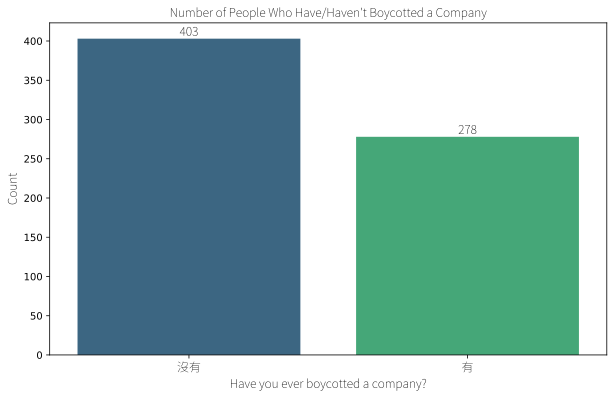
\includegraphics{_thesis_files/figure-pdf/cell-6-output-1.pdf}

\subsubsection{Why Boycott}\label{why-boycott}

\begin{longtable}[]{@{}lll@{}}
\toprule\noalign{}
& Reason & Count \\
\midrule\noalign{}
\endhead
\bottomrule\noalign{}
\endlastfoot
0 & 食安問題 & 33 \\
1 & 地溝油 & 10 \\
2 & 黑心油 & 8 \\
3 & 食安 & 5 \\
4 & 政治因素 & 4 \\
... & ... & ... \\
182 & 因為有出新聞 & 1 \\
183 & 此公司危害食安,以抵制這種行為讓公司更能意識到執行此行為的後果 &
1 \\
184 & 地溝油啊 & 1 \\
185 & 不認同理念 & 1 \\
186 & 因為這家公司壓榨員工 & 1 \\
\end{longtable}

\subsubsection{Trusted Brands}\label{trusted-brands}

\begin{longtable}[]{@{}lll@{}}
\toprule\noalign{}
& Brand & Count \\
\midrule\noalign{}
\endhead
\bottomrule\noalign{}
\endlastfoot
193 & No trusted brand & 329 \\
194 & Have but not specified & 56 \\
0 & 義美 & 42 \\
1 & Apple & 9 \\
2 & 光泉 & 7 \\
... & ... & ... \\
83 & 自家種植 & 1 \\
84 & Casetify & 1 \\
85 & Adidas & 1 \\
86 & 麥當勞 & 1 \\
97 & 淨毒五郎 & 1 \\
\end{longtable}

The following responses were counted as ``no brand'': ``無'', ``沒有'',
``沒有特別'', ``🈚️'', ``目前沒有'', ``No'', ``沒'', ``沒有特別關注'',
``沒有特別信任的'', ``不知道'', ``無特別選擇'', ``目前沒有完全信任的'',
``沒有特定的'', ``沒有特定'', ``沒有特別研究'',
``目前沒有特別關注的品牌'',``N'', ``none'', ``無特別'', ``目前無'',
``沒有特別想到'', ``沒有固定的'', ``x'', ``沒在買'', ``nope'',
``一時想不到\ldots{}'', ``沒有特別注意'', ``無特別的品牌'',
``無絕對信任的品牌'', ``不確定你說的範圍'', ``還沒有''

\subsection{Choice Experiments}\label{choice-experiments}

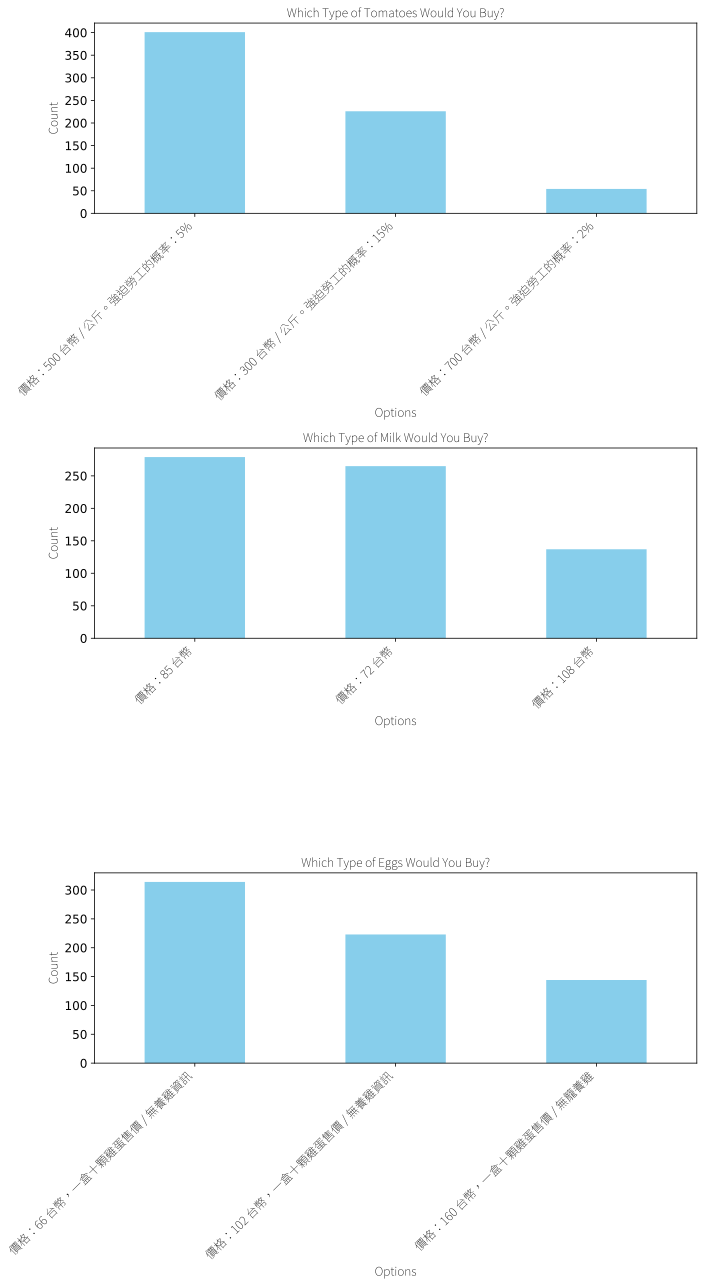
\includegraphics{_thesis_files/figure-pdf/cell-9-output-1.pdf}

\begin{center}\rule{0.5\linewidth}{0.5pt}\end{center}

title: Attitudes sidebar\_position: 3 execute: echo: false editor:
render-on-save: false suppress-bibliography: true

\begin{center}\rule{0.5\linewidth}{0.5pt}\end{center}

\section{College Student Attitudes
(Overall)}\label{college-student-attitudes-overall}

These are student attitudes across all 36 likert fields without
clustering. Clustered results are available under the Personas section.

\subsection{Shopping}\label{shopping-2}

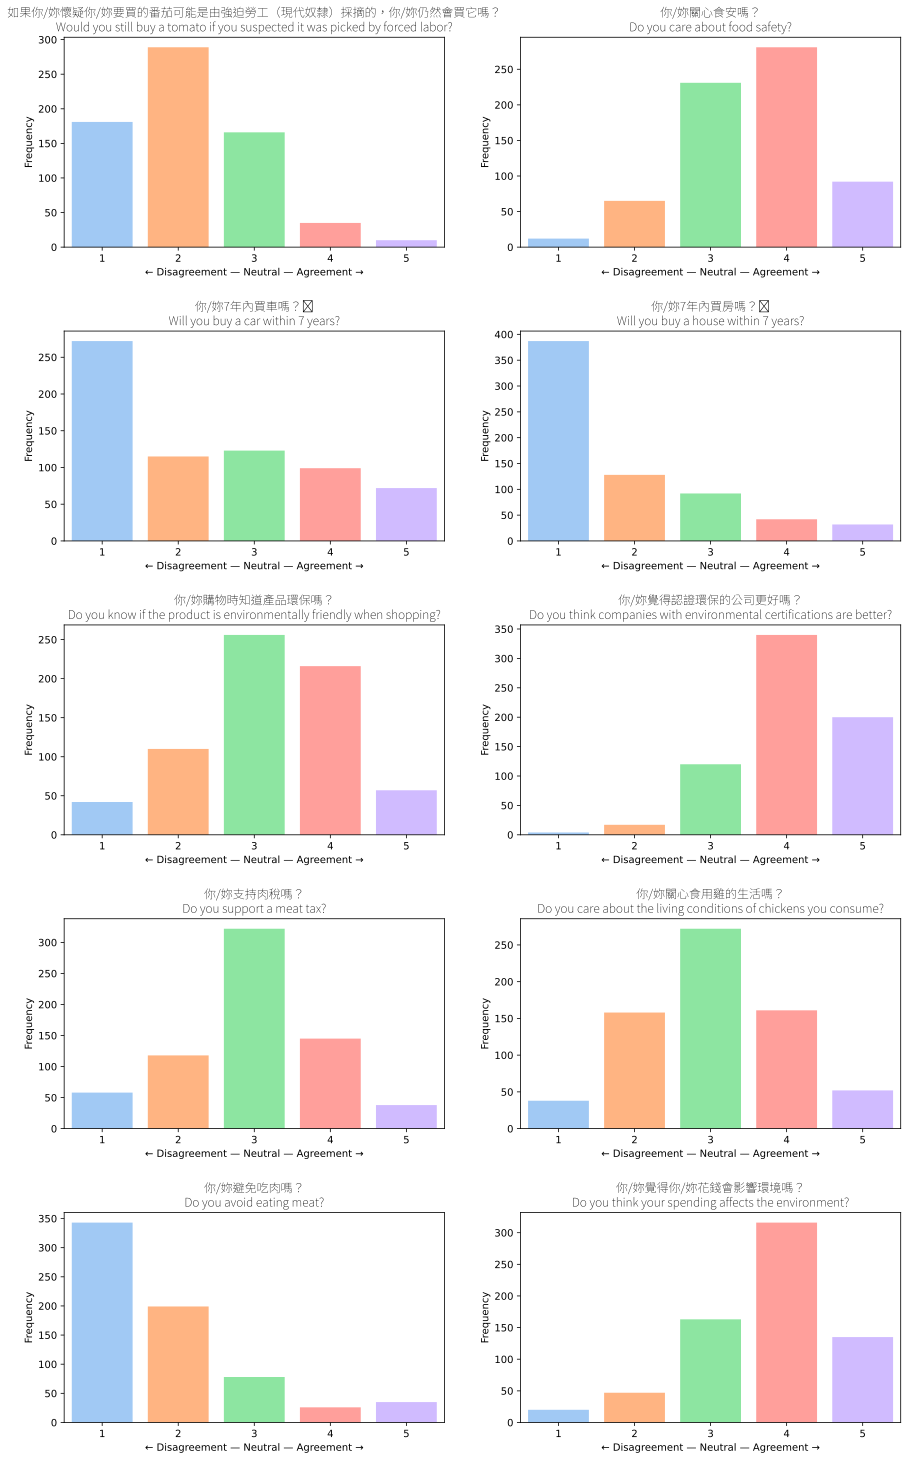
\includegraphics{_thesis_files/figure-pdf/cell-11-output-1.pdf}

\subsection{Saving and Investing}\label{saving-and-investing}

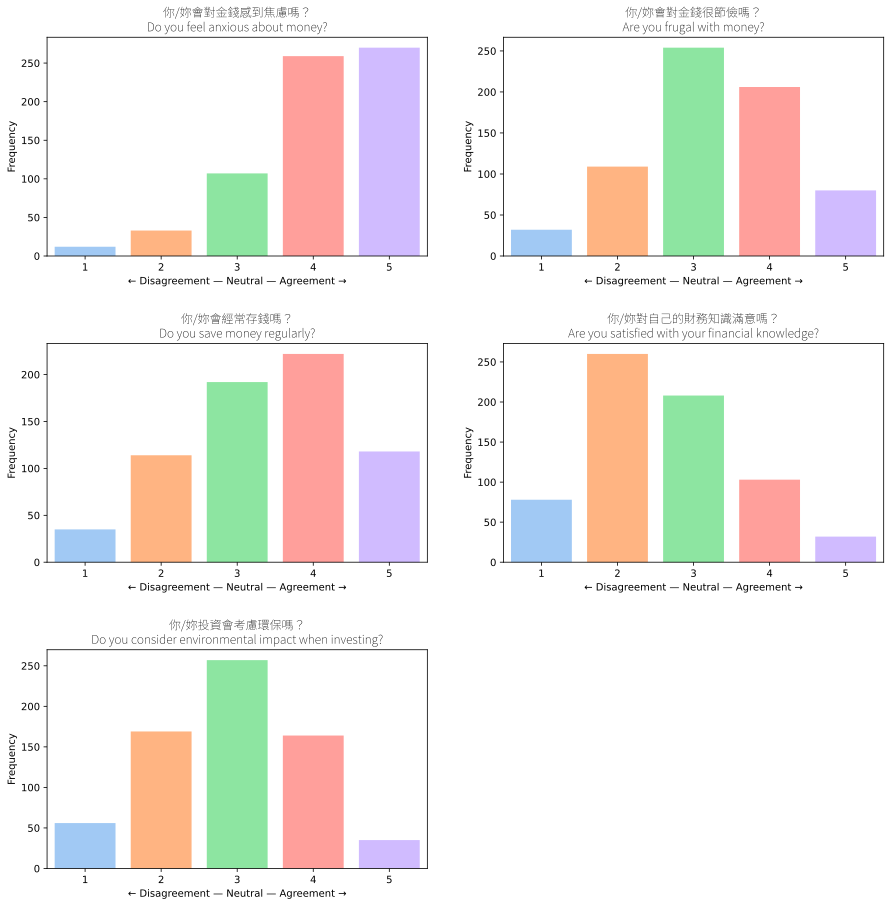
\includegraphics{_thesis_files/figure-pdf/cell-12-output-1.pdf}

\subsection{Economy}\label{economy}

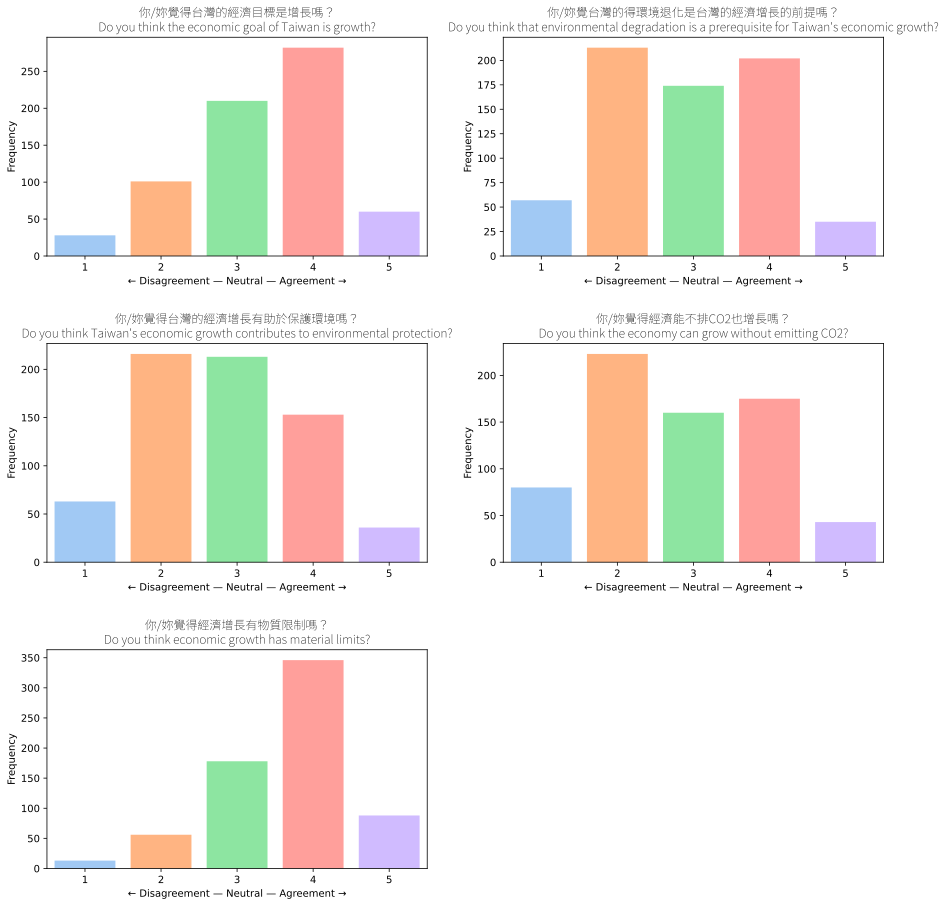
\includegraphics{_thesis_files/figure-pdf/cell-13-output-1.pdf}

\subsection{AI Usage}\label{ai-usage}

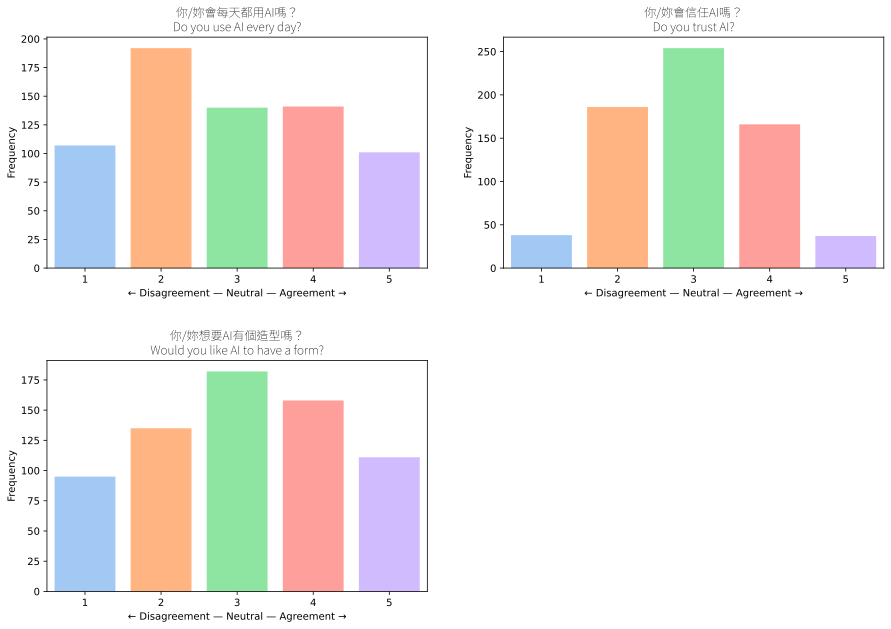
\includegraphics{_thesis_files/figure-pdf/cell-14-output-1.pdf}

\subsection{Nature}\label{nature}

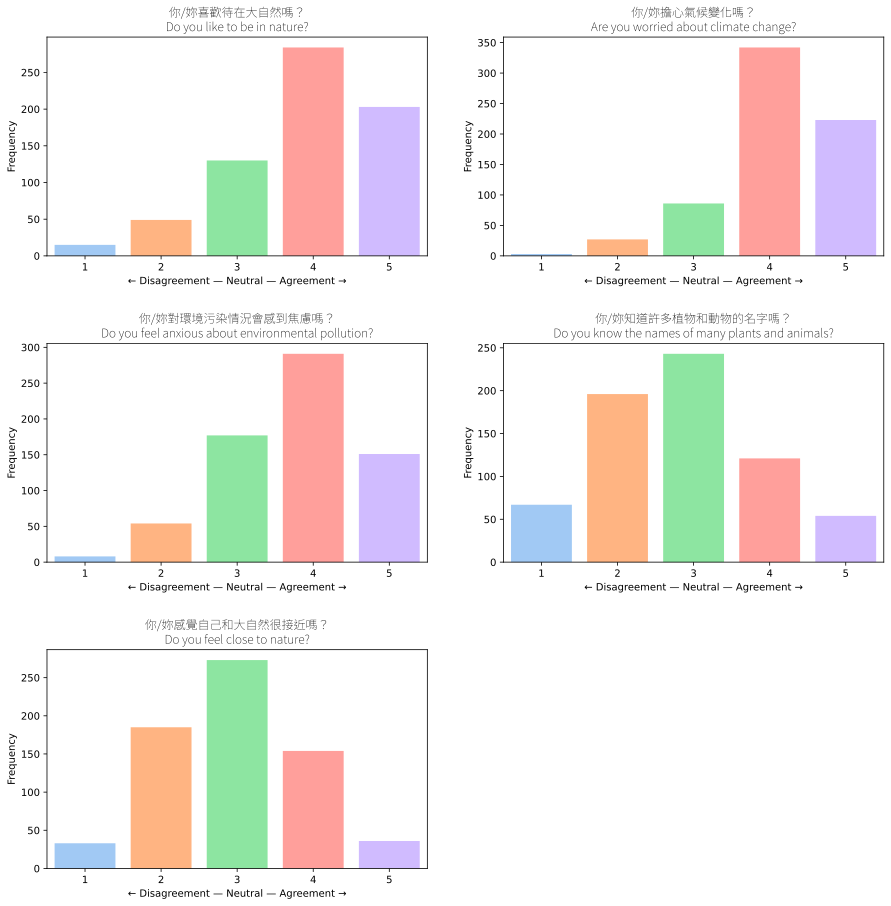
\includegraphics{_thesis_files/figure-pdf/cell-15-output-1.pdf}

\subsection{Environmental Protection}\label{environmental-protection}

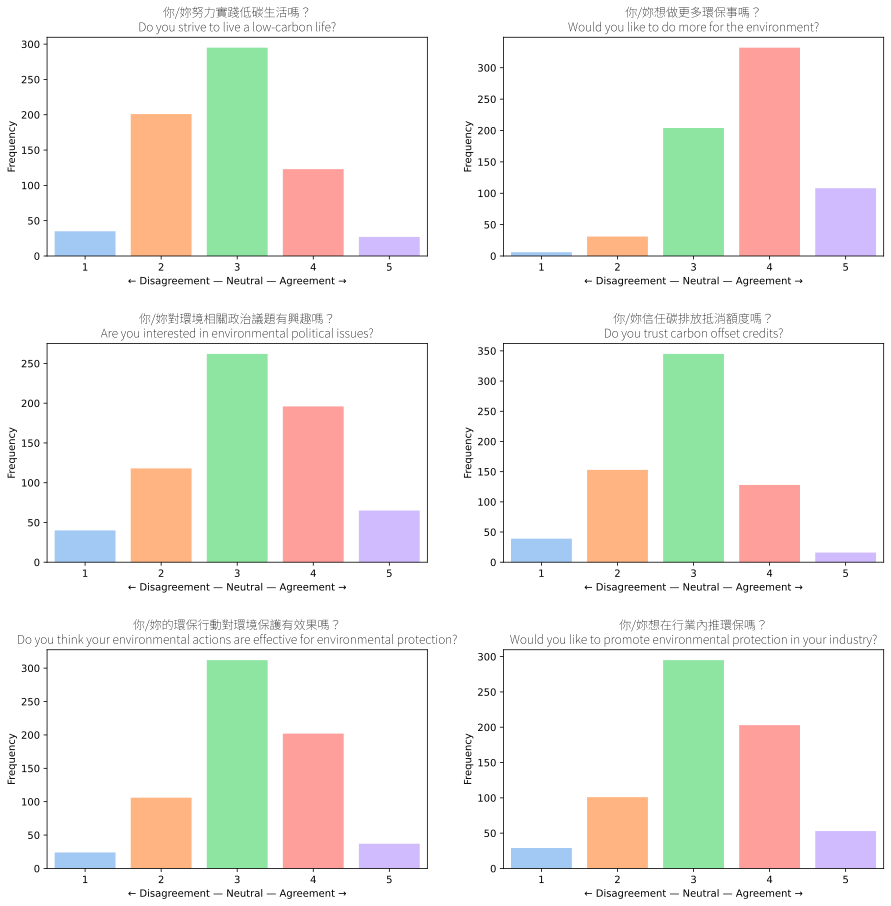
\includegraphics{_thesis_files/figure-pdf/cell-16-output-1.pdf}

\subsection{Learning Environment}\label{learning-environment}

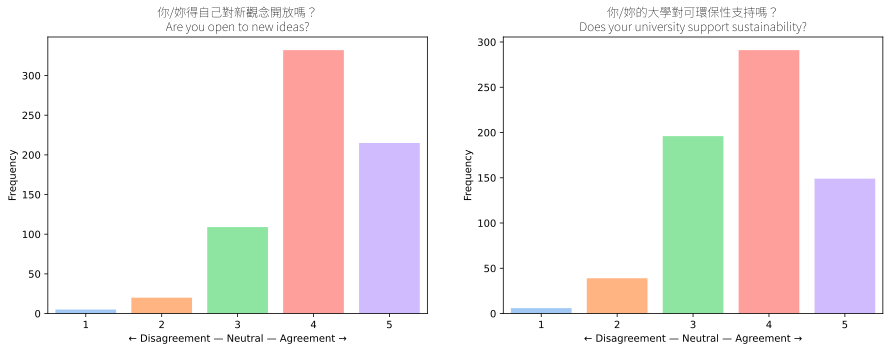
\includegraphics{_thesis_files/figure-pdf/cell-17-output-1.pdf}

\subsection{Correlations Between
Fields}\label{correlations-between-fields}

\includegraphics{_thesis_files/figure-pdf/cell-18-output-1.pdf}

\subsection{Environmental Knowledge Ranking
Experiment}\label{environmental-knowledge-ranking-experiment}

Test knowledge about the environment.

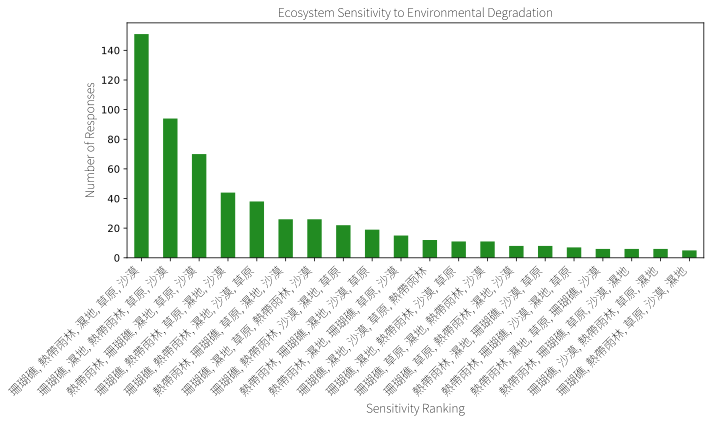
\includegraphics{_thesis_files/figure-pdf/cell-19-output-1.pdf}

\begin{center}\rule{0.5\linewidth}{0.5pt}\end{center}

title: Investing sidebar\_position: 3 execute: echo: false editor:
render-on-save: false suppress-bibliography: true

\begin{center}\rule{0.5\linewidth}{0.5pt}\end{center}

\section{Investing}\label{investing-1}

Student attitudes towards investing.

\subsubsection{Investing Experience
(Overall)}\label{investing-experience-overall}

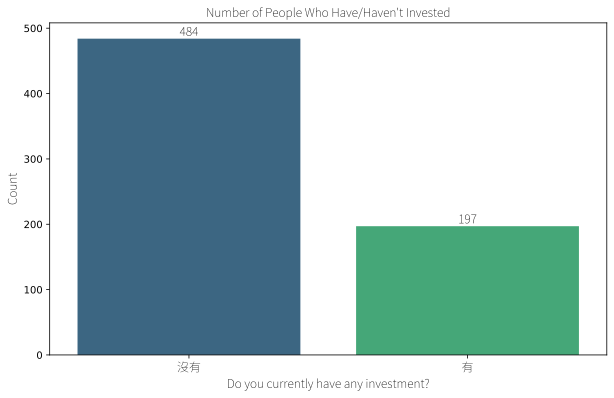
\includegraphics{_thesis_files/figure-pdf/cell-21-output-1.pdf}

\subsection{Choice Experiment}\label{choice-experiment}

Question: 你/妳選哪個投資?Which investment do you choose?

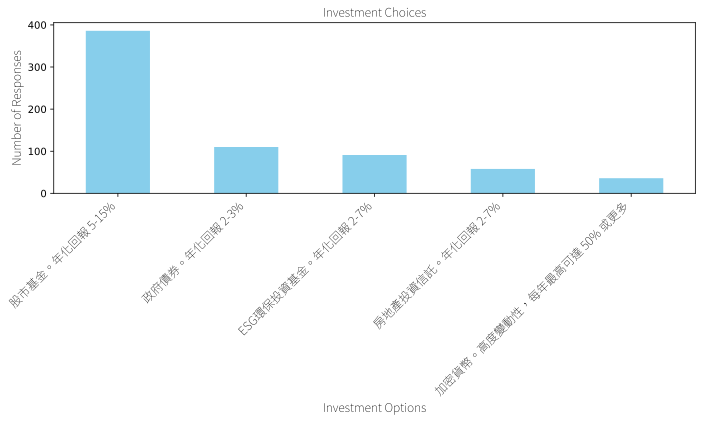
\includegraphics{_thesis_files/figure-pdf/cell-22-output-1.pdf}

\begin{center}\rule{0.5\linewidth}{0.5pt}\end{center}

title: Personas sidebar\_position: 3 execute: echo: false editor:
render-on-save: false suppress-bibliography: true

\begin{center}\rule{0.5\linewidth}{0.5pt}\end{center}

\section{Personas}\label{personas}

\subsection{Clustering Students to Build 3
Personas}\label{clustering-students-to-build-3-personas}

Personas are created using K-means clustering, an unsupervised machine
learning algorithm, which clusters college students based on their
responses across 36 Likert-scale fields in the online survey. Clusters
are visualized using Principal Component Analysis (PCA), where the
principal component loadings on the X and Y axes represent the weights
of the original Likert-scale fields, transformed into the principal
components that capture the most variance.

\begin{itemize}
\item
  There is some similarity between clusters. All 3 personas report a
  high level of financial anxiety and below-average satisfaction with
  their financial literacy.
\item
  Principal Component Analysis (PCA) is used to convert data to lower
  dimension space. This is a predecessor of embeddings.
\end{itemize}

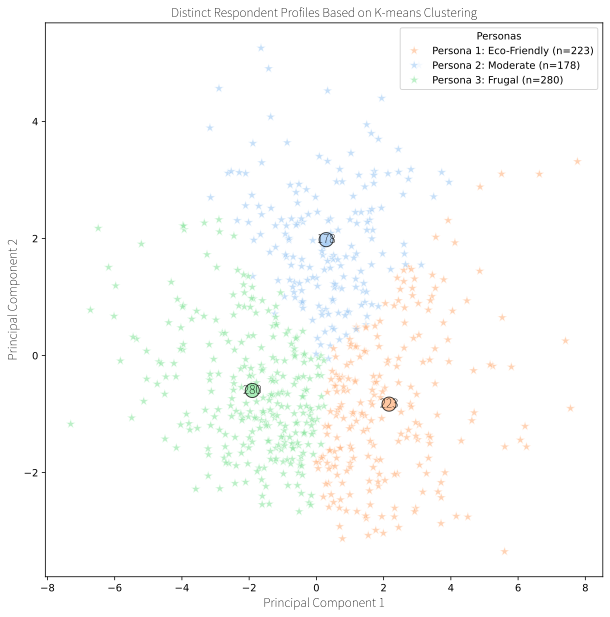
\includegraphics{_thesis_files/figure-pdf/cell-24-output-1.pdf}

\subsubsection{Persona 1:
``Eco-Friendly''}\label{persona-1-eco-friendly}

Questions Most Affecting Persona Creation include\ldots{}

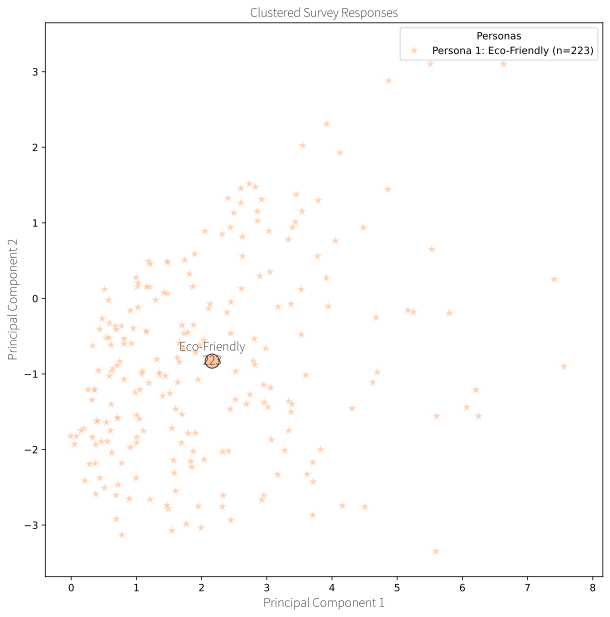
\includegraphics{_thesis_files/figure-pdf/cell-25-output-1.pdf}

\includegraphics{_thesis_files/figure-pdf/cell-25-output-2.pdf}

\includegraphics{_thesis_files/figure-pdf/cell-25-output-3.pdf}

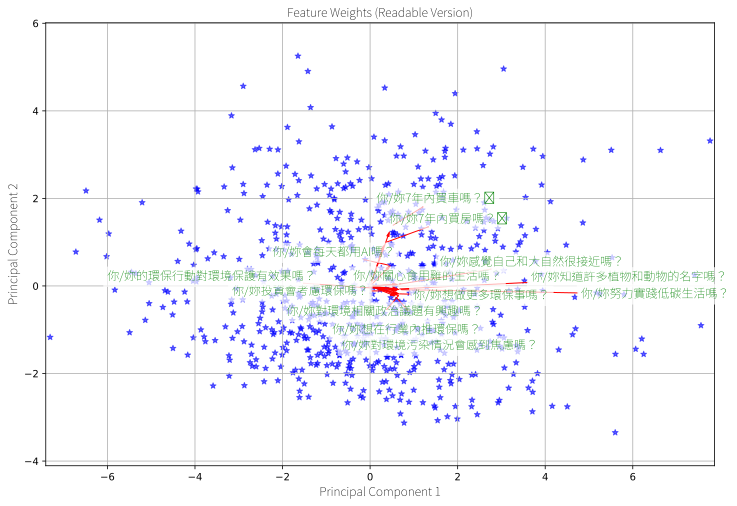
\includegraphics{_thesis_files/figure-pdf/cell-25-output-4.pdf}

\subsubsection{Persona 2: ``Moderate''}\label{persona-2-moderate}

Questions Most Affecting Persona Creation include\ldots{}

\includegraphics{_thesis_files/figure-pdf/cell-26-output-1.pdf}

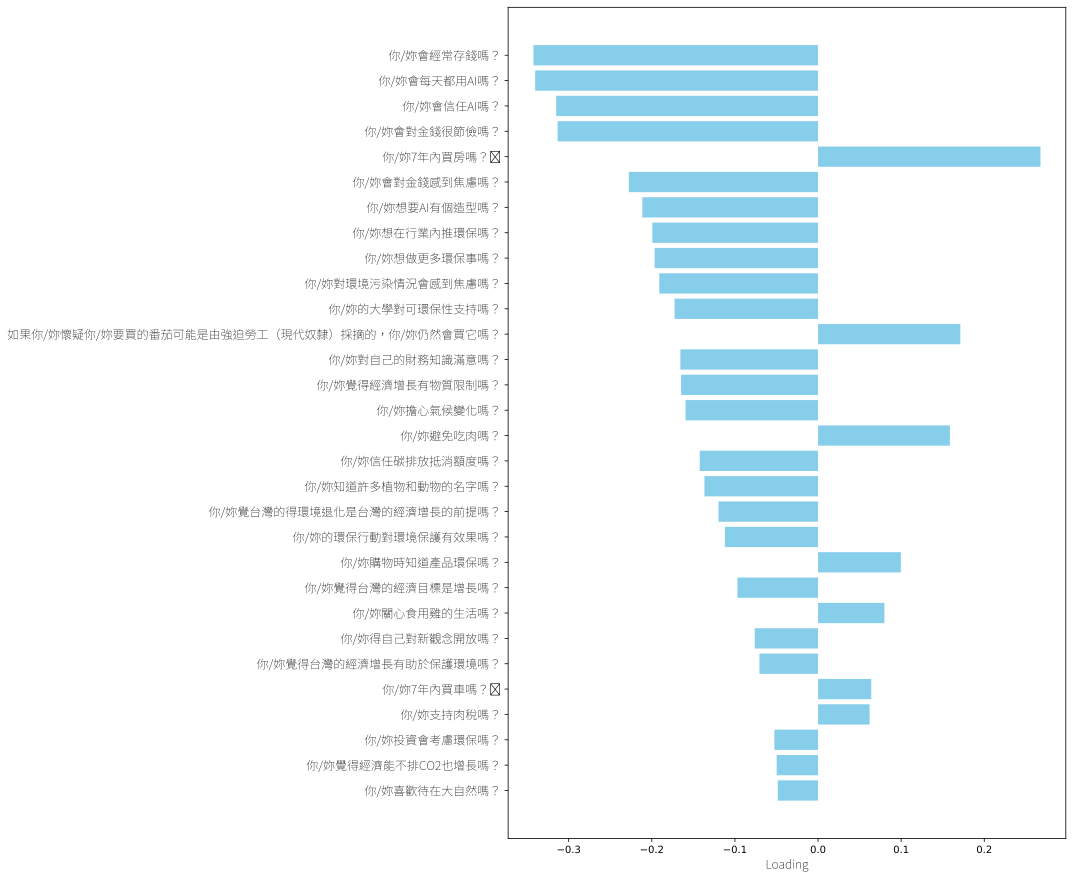
\includegraphics{_thesis_files/figure-pdf/cell-26-output-2.pdf}

\includegraphics{_thesis_files/figure-pdf/cell-26-output-3.pdf}

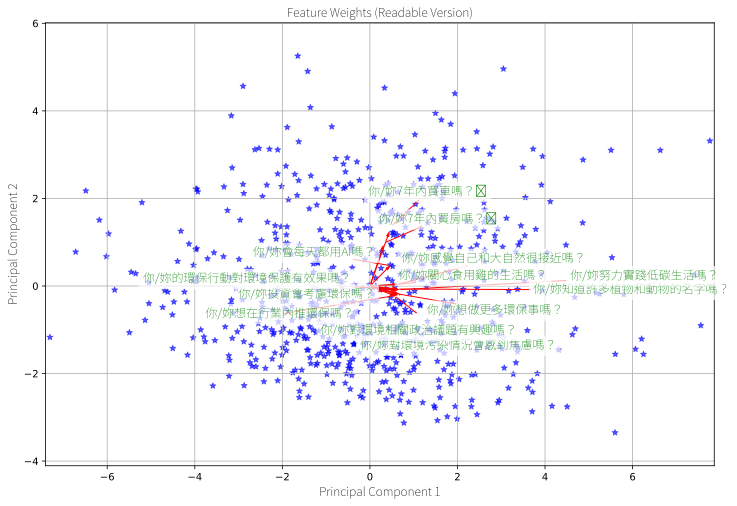
\includegraphics{_thesis_files/figure-pdf/cell-26-output-4.pdf}

\subsubsection{Persona 3: ``Frugal''}\label{persona-3-frugal}

Questions Most Affecting Persona Creation include\ldots{}

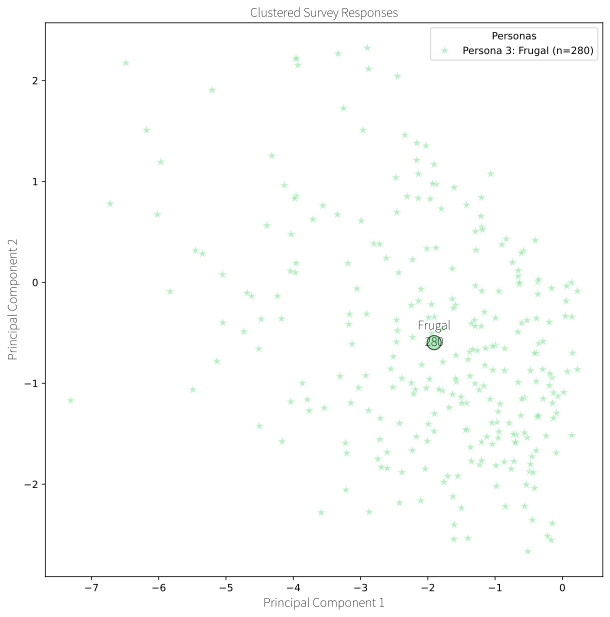
\includegraphics{_thesis_files/figure-pdf/cell-27-output-1.pdf}

\includegraphics{_thesis_files/figure-pdf/cell-27-output-2.pdf}

\includegraphics{_thesis_files/figure-pdf/cell-27-output-3.pdf}

\includegraphics{_thesis_files/figure-pdf/cell-27-output-4.pdf}

\subsection{Clustering Heatmap}\label{clustering-heatmap}

\includegraphics{_thesis_files/figure-pdf/cell-28-output-1.pdf}

\subsection{Mean Answer Scores}\label{mean-answer-scores}

Mean response values for each Likert question in each cluster:

\begin{longtable}[]{@{}llllllllllllllllllllll@{}}
\toprule\noalign{}
& Cluster &
如果你/妳懷疑你/妳要買的番茄可能是由強迫勞工(現代奴隸)採摘的,你/妳仍然會買它嗎?
& 你/妳關心食安嗎? & 你/妳7年內買車嗎?🚘 & 你/妳7年內買房嗎?🏡 &
你/妳購物時知道產品環保嗎? & 你/妳覺得認證環保的公司更好嗎? &
你/妳支持肉稅嗎? & 你/妳關心食用雞的生活嗎? & 你/妳避免吃肉嗎? & ...
& 你/妳知道許多植物和動物的名字嗎? & 你/妳感覺自己和大自然很接近嗎? &
你/妳努力實踐低碳生活嗎? & 你/妳想做更多環保事嗎? &
你/妳對環境相關政治議題有興趣嗎? & 你/妳信任碳排放抵消額度嗎? &
你/妳的環保行動對環境保護有效果嗎? & 你/妳想在行業內推環保嗎? &
你/妳得自己對新觀念開放嗎? & 你/妳的大學對可環保性支持嗎? \\
\midrule\noalign{}
\endhead
\bottomrule\noalign{}
\endlastfoot
0 & 0 & 2.026906 & 3.991031 & 2.206278 & 1.663677 & 3.681614 & 4.300448
& 3.434978 & 3.533632 & 2.269058 & ... & 3.381166 & 3.457399 & 3.426009
& 4.264574 & 3.820628 & 3.210762 & 3.645740 & 3.730942 & 4.403587 &
4.210762 \\
1 & 1 & 2.106742 & 3.516854 & 3.898876 & 2.904494 & 3.140449 & 4.028090
& 2.943820 & 3.117978 & 1.685393 & ... & 2.814607 & 3.039326 & 2.808989
& 3.679775 & 3.101124 & 2.865169 & 3.202247 & 3.117978 & 4.016854 &
3.719101 \\
2 & 2 & 2.214286 & 3.225000 & 1.575000 & 1.282143 & 2.853571 & 3.864286
& 2.642857 & 2.610714 & 1.600000 & ... & 2.453571 & 2.521429 & 2.446429
& 3.364286 & 2.739286 & 2.664286 & 2.792857 & 2.878571 & 3.850000 &
3.500000 \\
\end{longtable}

\subsection{Agreement between
personas}\label{agreement-between-personas}

Highest agreement between personas is about health, safety, pollution
and climate concerns.

\includegraphics{_thesis_files/figure-pdf/cell-30-output-1.pdf}

\begin{center}\rule{0.5\linewidth}{0.5pt}\end{center}

title: Features (AI) sidebar\_position: 7 execute: echo: false editor:
render-on-save: false suppress-bibliography: true

\begin{center}\rule{0.5\linewidth}{0.5pt}\end{center}

\subsection{AI Companion}\label{ai-companion}

\subsubsection{Likert-Based Clustering}\label{likert-based-clustering}

AI-assistant feature choices per Likert-based Personas

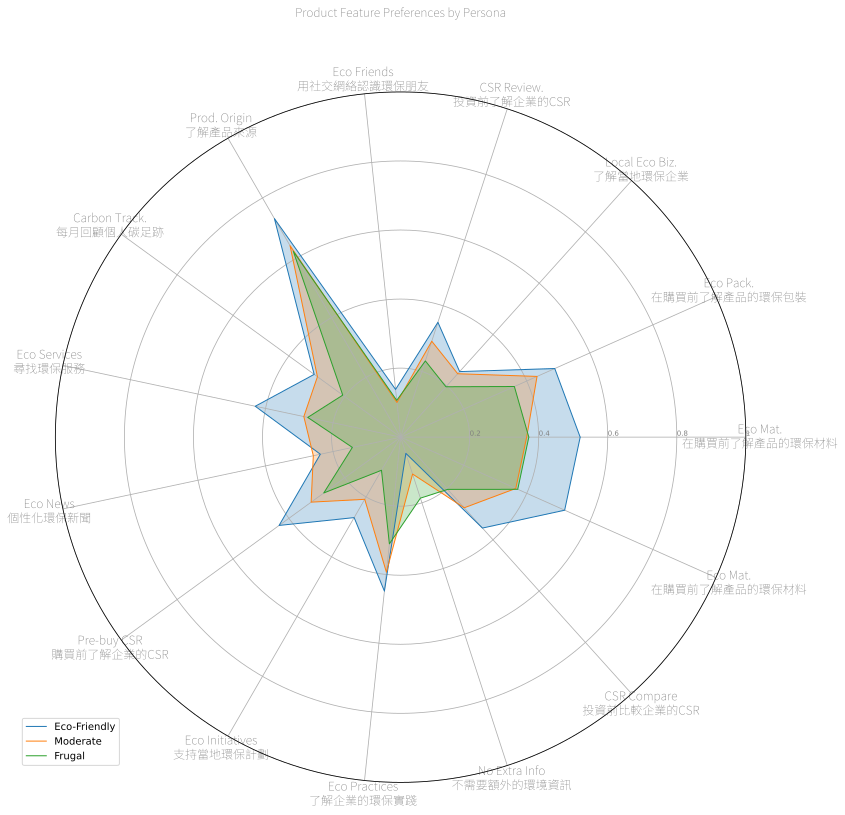
\includegraphics{_thesis_files/figure-pdf/cell-32-output-1.pdf}

Want: - Product origin - Product materials - Product packaging

Don't Want: - News - Carbon tracking - Eco-friends - \ldots{}

\subsection{Feature-Based Clustering}\label{feature-based-clustering}

Clustering students based on AI-assistant feature choices.

Want: - Product origin - Product materials - Product packaging - Eco
services

\subsubsection{Feature Preferences
(Overall)}\label{feature-preferences-overall}

\includegraphics{_thesis_files/figure-pdf/cell-33-output-1.pdf}

\subsection{Feature Preferences (By
Cluster)}\label{feature-preferences-by-cluster}

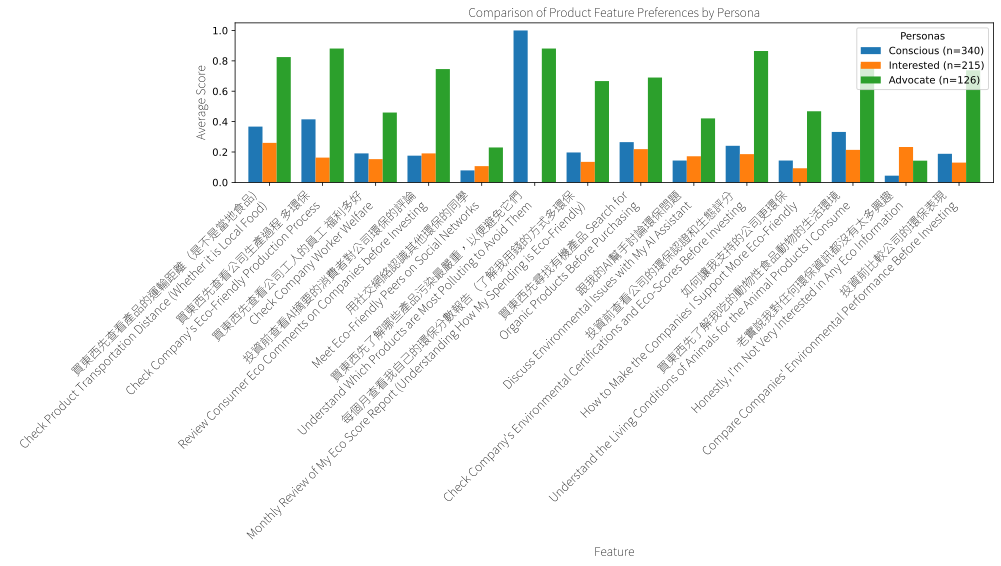
\includegraphics{_thesis_files/figure-pdf/cell-34-output-1.pdf}

\subsection{Preferred AI Roles
(Overall)}\label{preferred-ai-roles-overall}

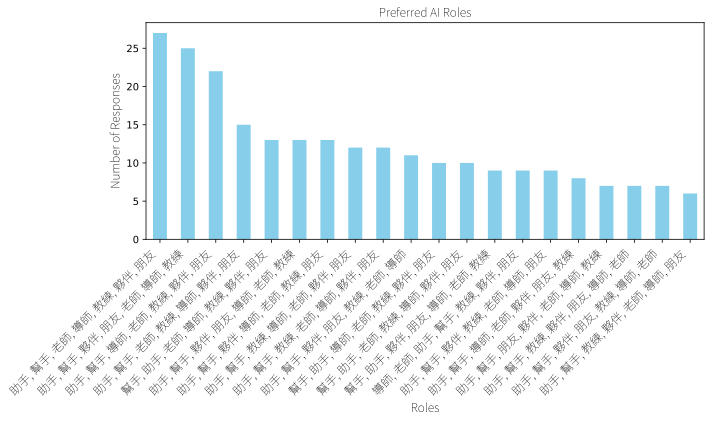
\includegraphics{_thesis_files/figure-pdf/cell-35-output-1.pdf}

\begin{center}\rule{0.5\linewidth}{0.5pt}\end{center}

title: Experts sidebar\_position: 7 execute: echo: false editor:
render-on-save: false suppress-bibliography: true

\begin{center}\rule{0.5\linewidth}{0.5pt}\end{center}

\subsection{Experts}\label{experts}

Analysis of recorded conversation

\newpage

\begin{center}\rule{0.5\linewidth}{0.5pt}\end{center}

title: Discussion sidebar\_position: 6 editor: render-on-save: false
suppress-bibliography: true

\begin{center}\rule{0.5\linewidth}{0.5pt}\end{center}

\section{Discussion}\label{discussion}

College Student Willingness to pay ( WTP)

Defining the Problem Space.

\subsection{Data Analysis}\label{data-analysis}

\begin{itemize}
\tightlist
\item
  Use K-Means clustering for survey data
\item
  K-means clustering is similar to vector distances for similarity used
  in large-language models (LLMs) word embeddings and deep learning.
\end{itemize}

\subsection{Mindmaps}\label{mindmaps}

Initial version of the concept map focused on the app itself.

Current concept map focusing on sustainability.

\subsection{Factorial Surveys}\label{factorial-surveys}

\begin{itemize}
\tightlist
\item
  \citet{li2022assessing}: ``Factorial surveys is a research method that
  combines classical experiments with survey methodologies. Factorial
  surveys use short narratives, called vignettes, to represent various
  levels of independent variables that are too complex or unethical to
  create and manipulate in real-world or lab situations''
\end{itemize}

\subsection{What is Research?}\label{what-is-research}

\begin{figure}[H]

{\centering \includegraphics[width=0.6\textwidth,height=\textheight]{./images/elephant.png}

}

\caption{Illustration of the Jainist parable Anekāntavāda also known as
``Blind Men and an Elephant''. Generated by Midjourney on August 17,
2023. Prompt: ``A simple pencil-drawn illustration of the the
story''Blind men and an elephant. The man touching the elephant's trunk
is a research scientist. Ohara Donshu, Itcho Hanabusa, Japanese woodcut
Edo style''}

\end{figure}%

\subsection{Research Through Design}\label{research-through-design}

\begin{itemize}
\tightlist
\item
  Design research books
\item
  \citet{koskinenDesignResearchPractice2011}
\item
  \citet{riesLeanStartupHow2011}
\item
  Design Studies Journal
\end{itemize}

\emph{Research through design} is a method for interaction design
research in Human-Computer Interaction (HCI).

\begin{itemize}
\item
  \citet{zimmermanResearchDesignMethod2007}
\item
  \citet{salovaaraHowDefineResearch2020} defining a research question
\item
  \citet{nunnallyUXResearchPractical2016}
\end{itemize}

interview people at google who made the green filter options

\begin{itemize}
\item
  Design artefacts
\item
  ``design's nature as a `problem-solving' science''
  \citet{oulasvirtaHCIResearchProblemSolving2016}
\item
  my contribution is the design artefact, ``HCI researchers also make
  constructive contributions by developing new technologies and design''
\item
  \citet{affairsCardSorting2013} Card sorting
\item
  \citet{HowModelsWork}
\item
  Behavirour kit:
\end{itemize}

Take the metrics from the several frameworks and display them on the
product and company level? People can choose their own framework and see
product data through that lens and vocabularies.

\begin{longtable}[]{@{}lll@{}}
\toprule\noalign{}
Col1 & Col2 & Col3 \\
\midrule\noalign{}
\endhead
\bottomrule\noalign{}
\endlastfoot
Donut Economy & Unrolled Donut & \\
Regenerative Capitalism & 8 Principles & \\
Blue Economy & & \\
ESG & & \\
B Corp & & \\
\end{longtable}

\begin{itemize}
\item
  ``research for design''. design research is about expanding
  opportunities and exploration
\item
  \citet{ranywayzResearchDesign2016}
\item
  \citet{mehmetaydinbaytasKindsDesignResearch2020}
\item
  \citet{047WordCreative}
\item
  \citet{KindsDesignResearch}
\item
  \citet{QualitativeVsQuantitative}
\item
  \citet{WhenUseWhich}
\item
  \citet{GreatUXResearch}
\item
  \citet{erikahallDesignResearchDone}
\item
  Contact Kalle Lasn, Culture Jam
\item
  online/offline ethnographic participant observation At this stage in
  the research, the central concept being studied is defined generally
  as user expectations for a sustainable investment app.
\item
  What are my hypotheses?
\item
  User experiments
\item
  Financial statistics
\item
  Analyzing existing apps and user pain-points
\item
  List of topics gleaned from literature review for discussion with the
  experts:
\item
  Transparency and sources of ESG and similar data
\item
  I will test the prototype with potential users using an online choice
  experiment survey.
\item
  Research Process In terms of literature review, academic inquiry in
  social sciences largely follows phenomena, while the issues and
  technologies discussed here are emergent. Not many studies exist yet
  (they might in a few years), which is why some of my references are to
  company press releases and news stories, or for public companies,
  their advisory for investors.
\item
  Target potential retail investors aged 20-29, all genders, in
  countries with highly developed financial markets and active social
  campaigns demanding sustainability (Sweden). And Taiwan. In general,
  the Taiwanese culture is savings oriented: I'm in a good location for
  financial user experience research.
\item
  Set your target goals
\item
  Access to health care
\item
  Access to education
\item
  Climate action
\end{itemize}

I propose \emph{interfaces} and \emph{workflows} to see financial
interactions through the filter of sustainability.

What kind of sustainability info do college students care about? How
would college students prefer to interact with the AI? What role would
college students prefer the AI to take? How can college students trust
AI? What can college students do to aid sustainability efforts? How
might AI assistants help college students find shopping, saving, and
investing opportunities?

``Systemic change through financial actions driving policy and market
changes encourage broader industry shifts towards greener practices''.

Overconsumption-driven extractive business practices contribute to the
degradation of Earth's natural ecosystems, pollution of water, air, and
soil, deforestation, diminishing biodiversity, climate instability,
extreme weather, modern slavery, worsening human health, and other
environmental and social challenges (ADD CITATION). Companies are
attuned to consumer demand however widespread greenwashing makes it
tiring to find sustainability-focused companies and requires extensive
time for research. Even for highly motivated people, it's difficult to
know what's sustainable.

My interest lies in understanding how AI assistants can help conscious
consumers become sustainable investors. The purpose of this study is to
explore how to provide the best user experience to potential sustainable
financial AI companion users. In their sustainability report every
company looks perfect. How can people shop, save and invest sustainably?
Where does our money go and what are some greener alternatives? The
companion enables people to be more transparent and responsible in their
consumption behavior.

in taiwan water is too pollutee can't swim

air is too dirty can't breather (show my own stats)

start local then go global with backup data from global sources

ask chatgpt how to organize my sections

rq: how to connect env destruction pollution to source causes

rq: how to connect everyday financial actions to environmental impact in
a visual/ meaningful way

idea came riding my bike in annan can't swim in yhe annan river

show local pollution map?

show factories on the map

instead of the browser pluging just make a website where you can share
the link of the product (and cache rhe results)

on ios can use the share screen to share to the app?

ICID calls upon us to have the courage to redesign entire industries

This research takes place at the intersection of Taiwanese college
students, sustainability, finance, AI, and design.

For the average person like myself, my experience with money is mostly
limited to buying things at the supermarket. Food, clothes, furniture,
soap, mobile phone. This leaves very few options on how to start with
something new like saving and investing.

Could the Green Supermarket become the entry point to Green Savings and
Green Investing?

Oboarding more people for sustainable practices is a complex interaction
design issue hindered by ambiguous data (what is sustainable?) and messy
human motivations (we love buying things).

What can people who want to preserve Earth's environment, exactly do?
How can networks of people come together?

--- LLMs enable data journalists to create stories:
\citet{biglocalnewsExpertShareSimon2024}

Health tracking apps paired with connected devices such as Apple Watch
filled with sensors provide one model for simple interactions to
dynamically track digital health data - also known as a quantified self.
This data allows apps to provide tips how to improve health outcomes
through small daily actions such as climbing more stairs. Small
interactions allow users to align their goals with their actions.

What would be a good interface to track sustainability? What is the user
interface at scale, useful for billions of people?

One way to influence societal outcomes is to decide where to put our
money. While our financial decisions are a vote towards the type of
businesses we want to support, is it enough?

While some people are demanding sustainability, and some governments and
companies are announcing green investment opportunities, how can
consumers discover the most suitable investment options for their
situation?

How can retail investors access and differentiate between eco-friendly
sustainability-focused investable assets?

The level of knowledge of and exposure to investing varies widely
between countries and people.

Could linking green consumption patterns with sustainable investing
provide another pathway to speed up achieving climate justice as well as
personal financial goals?

In this simplified scenario, I'm in a physical offline store, doing some
shopping. When putting a bottle of Coca Cola in my basket, my AI
companion Susan will ask me a personalized question:

Does individual climate action help?

Gen-Z college students (target users) may not have the capital to make a
financial dent today however they can be early adopter and they will be
the decision-makers in a few years.

``Like climate change, the focus on individual actions as a solution is
often misplaced, though it remains a focus of media and industry. For
decades, the petrochemical industry has offloaded responsibility onto
individuals through promoting concepts such as the''carbon footprint'',
championed in a 2004 advertising campaign by British Petroleum'' \citep[
in
\citet{laversFarDistractionPlastic2022}]{cherryProfitRethinkingCorporate2010}.

Individual efforts are too small to matter unless they're inspired by
Community a effort

atmospheric pollution and climate change

The latest IPCC report \citet{calvinIPCC2023Climate2023}

\citet{dimockDefiningGenerationsWhere2019}

\begin{itemize}
\item
  kora 95\% https://kora.app/
\item
  Earn KORA coins for reducing CO2 emissions
\end{itemize}

I, as the researcher, am similar to the blind people in the elephant
story; focusing on greening shopping, saving, and investing are only the
trunk of the enormous elephant that is environmental disaster unfolding
in front of our eyes.

\subsection{Results}\label{results-1}

The research helps me (and others) to

\begin{itemize}
\item
  avoid reinventing the wheel and duplicating existing approaches.
\item
  It aims to help app developers maximize impact by aiding complementary
  additionality.
\end{itemize}

\begin{itemize}
\tightlist
\item
  Make high-quality products. If used wisely, money can help build
  communities of sustainable impact.
\end{itemize}

\paragraph{Define Words}\label{define-words}

Define every word in the title: ``The Journey from Consumer to Investor:
Designing a Financial AI Companion for Young Adults to Help with
Sustainable Shopping, Savings, and Investing''

\begin{itemize}
\tightlist
\item
  Journey - behavioral change takes time
\item
  Consumer - purchase goods without thinking about the effect
\item
  Investor - thinking about the return
\item
  Design - decisions
\item
  Financial - dealing with money
\item
  AI Companion - automated sidekick
\item
  Young Adults - College Students
\item
  Help - to be of assistance
\item
  Sustainable Shopping - shopping understanding the consequences
\item
  Sustainable Saving - in this context I mean Sustainable Savings, that
  is reducing one's environmental footprint
\item
  Sustainable Investing - activity of thinking longer-term
\end{itemize}

\subsubsection{Open-ended Questions}\label{open-ended-questions}

\subsubsection{Close-ended Questions}\label{close-ended-questions}

\subsection{Expert Surveys}\label{expert-surveys}

\subsection{Database}\label{database}

Compile a database on relevant apps and companies in the space

Easily access data used in this research project (please wait a bit
until it loads below). The database includes sustainability-focused apps
categorized by features and problems they try to solve, sustainable
investing apps, and links to research papers.

\subsection{User Survey}\label{user-survey}

Start with a simple but powerful question: --- Does it matter what you
buy? --- Does it matter how much you save? --- Does it matter where you
invest? Why?

\subsection{Research Limitations}\label{research-limitations}

\begin{itemize}
\item
  This work is focused on user experience design and does attempt to
  make a contribution to economics. Sacred Economics is use as-is as a
  framework and visualization tool.
\item
  First, finance is a highly regulated industry and the proposed user
  experience designs may be limited by legal requirements. This study
  does not take such limitations into account, rather focusing only on
  the user experience.
\item
  Finally, ESG needs data to give us an accurate understanding of the
  realities inside companies and the user experience design does not
  address the underlying data quality problem further than by providing
  a link to the data source.
\item
  Research Reason: While many people are working on AI models, there's a
  lack of people working on ``Human-AI interaction''. Sustainability is
  the context. How can we better team up to solve the challenges we face
  this century? The huge externalities.
\item
  I don't have access to user financial data.
\item
  ESG data is expensive so couldn't be used in this research.
\end{itemize}

\subsection{Future Research}\label{future-research}

The literature is rich and there is ample space for future research. The
following includes some suggestions for authors whose work deserves a
deeper look.

\begin{itemize}
\tightlist
\item
  Does the specialized interface offer any advantages of a general UI
  such as ChatGPT, Claude, Gemini, Mistral, and others?
\end{itemize}

\newpage

\begin{center}\rule{0.5\linewidth}{0.5pt}\end{center}

title: Prototypes sidebar\_position: 7 editor: render-on-save: false
suppress-bibliography: true

\begin{center}\rule{0.5\linewidth}{0.5pt}\end{center}

\subsection{Prototypes of Product
Features}\label{prototypes-of-product-features}

I developed a number of early prototypes to visualize product feature
ideas.

What's on the intersection of College Students, Sustainability,
Investing, Data-Driven Design and Artificial Intelligence (AI)?
AI-Driven Sustainable Investment Tools.

The app aims to address the market failure by providing consumers
sufficient sustainability information on the goods, services and
investments.

resource depletion

and adopt the doughnut economy as my overarching theoretical framework

Humans are successful because of our adaptability. The study suggests
tools to adapt to our current reality.

United Nations Decade on Ecosystem Restoration

Hypothesis: extractive business practices reduce college students trust,
regenerative business practices create trust among college students
towards the company.

Provided there is awareness

How can sustainability-minded college students find companies that meet
their expectations, standards and requirements?

\begin{itemize}
\item
  Make a public profile of my carbon consumption!!! Like on Commons.
\item
  Shop
\item
  Save
\item
  Invest
\item
  Build closer relationships with sustainability-focused companies
\item
  Sales funnel for eco-focused products
\item
  The eco-friendly market is fragmented
\item
  Build trust, clarity, transparency, and honesty
\item
  Make a `Sustainability Flywheel' graphic, like that of Amazon's
\item
  Sustainability is fragmented. How can billions of people build closer
  relationships with sustainability-focused companies based on honesty
  and transparency? A research project for designing a sustainable
  shopping, savings, and investing companion.
\item
  Most sustainability plans rely on carbon credits to achieve their
  goals, making carbon credits a single point of failure. If the credits
  are not accurate, the whole system collapses.
\item
  TODO: Make a table showing research results translated to design
  decisions
\item
  Your Green Helper
\item
  Make some initial prototype? make YoutTbe video\ldots{} hi, you have
  reached? spread\ldots{} through ESTBan and others?
\item
  Currently CO\textsubscript{2} footprint calculators ask you a couple
  of questions and give a ballpark estimate. Does it make sense to track
  sustainability on a more nuanced level, like Apple Health, in order to
  encourage sustainable behavior?
\end{itemize}

\begin{longtable}[]{@{}
  >{\raggedright\arraybackslash}p{(\columnwidth - 6\tabcolsep) * \real{0.2466}}
  >{\raggedright\arraybackslash}p{(\columnwidth - 6\tabcolsep) * \real{0.2466}}
  >{\raggedright\arraybackslash}p{(\columnwidth - 6\tabcolsep) * \real{0.2466}}
  >{\raggedright\arraybackslash}p{(\columnwidth - 6\tabcolsep) * \real{0.2603}}@{}}
\toprule\noalign{}
\begin{minipage}[b]{\linewidth}\raggedright
Product Idea
\end{minipage} & \begin{minipage}[b]{\linewidth}\raggedright
Source
\end{minipage} & \begin{minipage}[b]{\linewidth}\raggedright
\end{minipage} & \begin{minipage}[b]{\linewidth}\raggedright
Prototype Link
\end{minipage} \\
\midrule\noalign{}
\endhead
\bottomrule\noalign{}
\endlastfoot
Speak Truth to Power & Literature Review & Consolidate user feedback for
companies & greenfilter.app/prototypes/truth-power \\
Shopping Divest & Literature Review & What if you could build
communities based on what you buy? &
greenfilter.app/prototypes/shopping-divest \\
True Cost & Literature Review & What if you could see the actual cost of
each product including externalities? &
greenfilter.app/prototypes/true-cost- \\
Sunday Market & Literature Review & First prototype for going to the
organic Sunday Market with friends. & \\
XYZ & Expert Interview & & \\
ABC & User Survey & & \\
\end{longtable}

\subsection{Affinity Diagrams}\label{affinity-diagrams}

\begin{itemize}
\tightlist
\item
  Affinity diagrams help users organize ideas by brainstorming, sorting
  and labeling to cluster related information
  \citep{karaperniceAffinityDiagrammingCollaboratively2018, quignardUXAnalysisPhase2022}
\end{itemize}

Scan a product to see the company and start investing or divesting from
them Current economics is lowering the quality of life on the planet

Actionable Insights: Translate data into everyday actions the app can
suggest.

\begin{itemize}
\tightlist
\item
  What does investing look like at the scale of billions of people? like
  IG
\item
  The most effective things are Commodities? Food, transport, fashion,
  plant trees.
\item
  personalized AI, meta glasses understand your context. sense and
  reconstruct the world around you and to understand the context in
  which you're using your device.sense and reconstruct the world around
  you and to understand the context in which you're using your device.
  Make suggestions and take action proactively to help you get things
  done --- ideally, so seamlessly that you may not even
  notice.neuroscience co-adaptation of the interface. your future
  devices will learn and adapt to you as you use them.
\item
  Scalable Climate Solutions: What really works on a large scale?
\item
  brand colors: pink, orange, green
\end{itemize}

\subsection{Shopping-as-Investing}\label{shopping-as-investing}

\begin{itemize}
\item
  Introduce this concept
\item
  \citet{themanorSustainabilityNotSacrifice2022}
\item
  Sustainability is hard. Green Filter helps you find companies that are
  making a true effort and build closer relationships through shopping,
  savings, and investing. Green Filter helps you find companies that are
  making a true effort to become sustainable and build closer
  relationships through shopping, savings, and investing
\item
  Gather requirements and build a prototype for the next-generation
  investment app for young adults. Improving the user experience for
  young adults getting started with (green) investing. What would a
  ``Tinder for (Green) Investments'' look like? How can we make the
  logistics of investing so easy to use and take into account my values?
\item
  My thesis core message is : everyone should change from consumer to
  sustainability investor (define these terms in the thesis). how to do
  this? can help you become from consumer to investor i believe there's
  space for a product like that. your green investing friend find the
  companies tackling certain problems and invest in them using crypto
  business can be a force for good
\end{itemize}

\subsection{`Shopping-as-Investing'}\label{shopping-as-investing-1}

\begin{itemize}
\tightlist
\item
  Consumer purchases are an indicator of demand. If demand trends down,
  companies will stop producing this product.
\end{itemize}

\subsection{`Investment-as-Product'}\label{investment-as-product}

\begin{itemize}
\item
  Green Filter helps you discover how to save money and the planet with
  your daily shopping. By providing an easy way for people to learn
  about and shop with sustainable companies, we imagine a world where
  people invest in their future, find great deals on responsibly-made
  products, and get useful discounts from socially responsible brands.
\item
  GreenFilter is a product that combines AI, design and marketing to
  help people manage their social impact throughout the stages of their
  lives, from young adult years to retirement. Its primary goal is to
  give people the tools they need to invest responsibly in sustainable
  companies, while also educating them on this topic. Our project offers
  a responsive website and mobile app that leverages AI and other
  advanced technologies. In addition, our prototype includes a
  reality-based virtual assistant with voice command capabilities which
  can provide customers with new insights into the world of green
  finance
\item
  GreenFilter introduces a novel, interactive point-of-sale technology
  that helps people make greener shopping decisions. The platform uses
  artificial intelligence to suggest green alternatives for products on
  your shopping list, and will also help you to find other companies
  that can make sustainable versions of the product you are buying.
\item
  As people become aware of the impact their shopping is having on the
  environment, they become interested in finding alternatives to big
  brands and large companies. GreenFilter provides designers an AI
  companion design which helps people build relationships with
  sustainability-focused companies by providing personalized
  recommendations, giving product reviews and helping them shop
  sustainably. This new tool will empower consumers to make greener
  choices throughout their lives.
\item
  Better management of planet Earth
\item
  How can wee Shop, Save, Invest in line ecologic principles and
  planetary boundaries? individual action doesn't move the needle. how
  to group together
\item
  App to build community
\item
  Life within planetary boundaries
\item
  Currently it seems there's a secret around how things are produced we
  want to increase transparency
\item
  Companies that have nothing new nothing to hide should welcome this
  opportunity to mark themselves to keep a conscious consumers and
  investors.
\item
  We want to create competition around sustainable practices enter
  widespread adoption
\item
  Cigarettes and pictures of lung cancer every product should be
  required to have photos of production conditions switch such as
  Rainforest and deforestation the products that include Palm oil.
\item
  My thesis is that a lot of people want to do good, shop eco-friendly,
  invest green, etc. But they don't believe the solutions work. They
  don't have trust. This is a user interface issue. How to build trust.
\end{itemize}

\begin{center}\rule{0.5\linewidth}{0.5pt}\end{center}

title: Early Feature Ideas sidebar\_position: 1 editor: render-on-save:
false suppress-bibliography: true

\begin{center}\rule{0.5\linewidth}{0.5pt}\end{center}

\section{Early Feature Ideas}\label{early-feature-ideas}

The following early prototypes are focused on particular feature ideas
that occurred to me during the literature review process. They are naive
and meant to allow thinking in terms of \emph{what-if} a particular user
experience was possible. These prototypes were not tested with users
directly and formed a basis for directing the questions asked in a
potential user survey.

\section{Susan (Sustainability
Conversation)}\label{susan-sustainability-conversation}

\emph{What if} I could have a chat like this at the supermarket? Imagine
what questions I would ask before buying a product. AI: ``Kris, do you
still remember Coca Cola's packaging is a large contributor to ocean
plastic? You even went to a beach cleanup!'' Me: ``That's so sad but
it's tasty!'' AI. ``Remember your values. Would you like to start saving
for investing in insect farms in Indonesia instead? Predicted return 4\%
per year, according to analysts A and B.'' If I'm not so sure, I could
continue the conversation. Me: ``Tell me more'' AI: ``A recent UN study
says, the planet needs to grow 70\% more food in the next 40 years.
Experts from 8 investment companies predict growth for this category of
assets.'' Me: ``Thanks for reminding me who I am'' \ldots{} Moments
later. AI: ``This shampoo is made by Unilever, which is implicated in
deforestation in Indonesia according to reporting by World Forest Watch.
Would you consider buying another brand instead? They have a higher ESG
rating.''

Example Suggestions of the AI companion:

\begin{itemize}
\item
  ``Don't buy a car, use a car sharing service instead to save XYZ CO2.
  Service available near you: Bolt,* Uber.''
\item
  ``Use a refillable shampoo bottle to save XYZ plastic pollution''
\item
  ``Call your local politician to nudge them to improve bicycle paths
  and reduce cars in your neighborhood. Over the past 2 years, you city
  has experienced an increase of cars from 290 cars per capita to 350
  cars per capita.''*
\end{itemize}

Figure 3: Speculative scenario of an interaction between a human user
and a robo-advisor through the interface of chat messages in the context
of retail shopping for daily products.

https://scontent.ftpe6-1.fna.fbcdn.net/v/t39.8562-6/333078981\_693988129081760\_4712707815225756708\_n.pdf

provides many examples conversations between AI and humans from Meta's
LLAMA mmodel

\begin{figure}[H]

{\centering \includegraphics[width=0.5\textwidth,height=\textheight]{./images/susan-pink-app.png}

}

\caption{Early prototype of my Sustainable Finance AI Companion
(Nov.~2020)}

\end{figure}%

\subsection{Sunday Market}\label{sunday-market}

\emph{What if} I could go to the Sunday market with other people who
care about sustainability? First prototype (based on literature review)
called HappyGreen's for going to the organic Sunday Market with friends.
Choose industries of focus? Fashion, Food, etc?

\subsection{True Cost}\label{true-cost}

\emph{What if} I you could see the actual cost of each product including
externalities?

\subsection{Speak Truth to Power}\label{speak-truth-to-power}

\emph{What if} I could affect companies with truth? Consolidate user
feedback for companies.

\subsection{How Far?}\label{how-far}

\emph{What if} I knew how far did this product travel to reach me?

\subsection{Country Profiles}\label{country-profiles}

\emph{What if} I knew my country's top pollution sources?

\subsection{Know Your Company}\label{know-your-company}

\emph{What if} I could KYC the companies I interact with? Like the banks
KYC, consumers can KYC.

\subsection{CO2e Flex}\label{co2e-flex}

\emph{What if} I could show off how much CO2e I have retired?

\subsection{Sustainability Watch}\label{sustainability-watch}

\emph{What if} I could see all my sustainability data on a wearable
device in the right context?

\subsection{Narrative Layouts}\label{narrative-layouts}

\emph{What if} I spent 5 minutes every day with a guide who could help
me make more eco-friendly choices? How should the layout storyline be
structured? Well it's like Strava (that running app) for
sustainability\ldots{} or if you have heard of Welltory. I believe
sustainable choices that would improve my life.. be it what I consume,
save, invest, etc.. so I'm trying to design an app around this idea. I'm
basically building the UX of AI.. focused on sustainability. How should
the layout storyline be structured? Well it's like Strava (that running
app) for sustainability\ldots{} or if you have heard of Welltory. I
believe if I spent 5 minutes every day with a guide who could help me
make more eco-friendly choices that would improve my life.. be it what I
consume, save, invest, etc.. so I'm trying to design an app around this
idea.

\subsection{Shopping Divest}\label{shopping-divest}

\emph{What if} I you could build a community based on what I buy?

\subsection{Books Can Talk}\label{books-can-talk}

\emph{What if} sustainability literature could chat with me? Books can
now talk to me. My bedtime story about shopping, saving, and investing.
\citep{SustainableShoppingSaving2023}

\begin{itemize}
\tightlist
\item
  \citep{raykurzweilIntroducingSemanticExperiences2018}
\item
  \citep{baileyAIEducation2023}
\end{itemize}

\begin{center}\rule{0.5\linewidth}{0.5pt}\end{center}

title: Interactive Prototype sidebar\_position: 1 editor:
render-on-save: false suppress-bibliography: true

\begin{center}\rule{0.5\linewidth}{0.5pt}\end{center}

\section{Interactive Prototype}\label{interactive-prototype}

\begin{itemize}
\tightlist
\item
  https://ai.ziran.tw/
\item
\end{itemize}

\subsection{Testing}\label{testing}

\subsection{Retrieval-Augmented Generation
(RAG)}\label{retrieval-augmented-generation-rag}

\begin{itemize}
\tightlist
\item
  ``make contextual decisions on-the-fly, thereby opening up a more
  dynamic and responsive way to handle knowledge search tasks''
  \citet{dewyBuildingRAGTool2024}
\end{itemize}

\subsection{Prototype Development}\label{prototype-development}

-- tools used: qr generator in Canva postman for API testing

\begin{itemize}
\item
  Google Chrome has 3.45 billion users
  \citet{GoogleChromeStatistics2023}
\item
  Retrieval-Augmented Generation (RAG) to enhance AI content with
  domain-spefic (close-to realtime) knowledge.
\item
  technique first proposed by researchers at META
  \citep{lewisRetrievalAugmentedGenerationKnowledgeIntensive2020} some
  RAG benefits include
  {[}\citet{gaoRetrievalAugmentedGenerationLarge2023};{]}
\end{itemize}

Prototype architecture

\begin{itemize}
\item
  Google Chrome browser extension
\item
  ApI microservice
\item
  Ziran AI
\item
  AI backend
\item
  Ratings API
\item
  Redis testing ai results
\item
  Redis Page cache / from page / separate scraping service
\item
  documentation: GreenFilter: thesis website / github
\item
  Ai Api got / claude
\item
  Stock ratings API
\item
  Community ratings api
\end{itemize}

70 qeustions questionairw - use report ID to do anonymois teating - page
tracking to track the usage - 7 app wuestions - 63 pwrsonality wuestion

\begin{center}\rule{0.5\linewidth}{0.5pt}\end{center}

title: Testing sidebar\_position: 8 execute: echo: false editor:
render-on-save: false suppress-bibliography: true

\begin{center}\rule{0.5\linewidth}{0.5pt}\end{center}

\section{Testing}\label{testing-1}

Does the prototype match user needs?

\subsection{App Testing Flow}\label{app-testing-flow}

\begin{figure}[H]

{\centering \includegraphics[width=1\textwidth,height=\textheight]{./images/app-testing-flow.png}

}

\caption{App Testing Flow}

\end{figure}%

\subsection{Testing Period}\label{testing-period}

\begin{itemize}
\tightlist
\item
  1 month from 2024 April 2 to May 2, 2024
\item
  30 individual participants
\end{itemize}

\subsection{Testing}\label{testing-2}

Prototype Testing results

sun, 14. april. 22h at D24

\begin{itemize}
\tightlist
\item
  ncku student, gen-z
\item
  searches for lancome brand
\item
  chooses LANCOME 蘭蔻 小黑瓶100ml(買一送一/超未來肌因賦活露國際航空版)
  https://www.momoshop.com.tw/goods/GoodsDetail.jsp?i\_code=12028429\&Area=search\&oid=1\_8\&cid=index\&kw=lancome
\item
  notices 買一送一
\item
  doesn't notice analysis button at first
\item
  would only click on this if it's really expensive
\item
  would not click on ``continue chat button''
\item
  asked ``why is it so expensive in taiwan2
\item
  considers report result useful
\end{itemize}

note: there's dropoff on evey step of the user journey

RQ: To what extend can shopping become and entry point for saving and
investing. RQ: Can shopping serve as an entry point for sustainable
saving and investing?

Testing overview

\begin{itemize}
\tightlist
\item
  Tested with 30 participants individually
\item
  Testing is anonymous
\item
  Generate
\item
\end{itemize}

有意識的消費主義

\begin{itemize}
\tightlist
\item
  add carbon indicators, other labels to the analsysi, add report code,
  calculate report code from URL? ssave as kv
\end{itemize}

\begin{longtable}[]{@{}
  >{\raggedright\arraybackslash}p{(\columnwidth - 0\tabcolsep) * \real{0.0417}}@{}}
\toprule\noalign{}
\endhead
\bottomrule\noalign{}
\endlastfoot
may 8 czuta \\
- investment help useless.. needs simpler intro - wants to see real cows
- very curious abouut companes - wants to see profit percentage. why is
margin so high if polluution is bad. - real environmental impact of the
coompany. \\
\end{longtable}

06 may - Seeing factory photos is useful only if they are trustworthy
photos. Who will provide them? -

\begin{center}\rule{0.5\linewidth}{0.5pt}\end{center}

may 5 - user: it looks like an ad -

\begin{longtable}[]{@{}l@{}}
\toprule\noalign{}
\endhead
\bottomrule\noalign{}
\endlastfoot
may 3 \\
- uses google to look for ``fashion brand eco friendly'' \\
- thinks ``goodonyou.eco'' looks like a brand website \\
\end{longtable}

\begin{longtable}[]{@{}
  >{\raggedright\arraybackslash}p{(\columnwidth - 0\tabcolsep) * \real{0.0694}}@{}}
\toprule\noalign{}
\endhead
\bottomrule\noalign{}
\endlastfoot
may3 - first looked for NET clothes but Momo doesn't sell it - Looked
for Sony camera lens \\
\end{longtable}

1 may prof suggestion - make connection between biodibersity and
production and consumption clearer - what is the incentive for companies
to share their data?

my own idea: like the switch of going from traditional banking with ATM
machines on the street (or even the physica bank office) to online
banking with mobile payments

\begin{itemize}
\item
  hypothesis: esg accessibility can push companies to increase
  production standards
\item
  what if you can see ESG in near-realtime such as the stock market
  price
\item
  i can imagine esg derivative product like siemens gamesa
\item
  ai can help integrate esg derivatives into daily life to drive esg
  adoption
\item
  ``effective altruism (EA)''
\item
  ``Blockchain technology can improve price transparency in product
  distribution by allowing consumers to know the exact pricing from raw
  materials to distributors to suppliers.''
\item
\end{itemize}

Interviews and testing survey were conducted anonymously in hopes to
have more honest responses from the responders.

\begin{itemize}
\tightlist
\item
  ziran chrome extension is unable to record activity due to browser
  security restrictions for plugins
\item
  ai.ziran.tw record user activity
\item
  semi-structured interviews were conducted in chinese
\item
  the interviewer (me) took notes of the interviews
\item
  some gaps in the data exist due to the limited chinese language skills
  of the interviewer (me)
\end{itemize}

basic interview script - momo: what is a brand that you like'd or would
like to buy - search - please pick a product (or search again) - on
product page: what do you notice on this page? - what kind of
information is important for you on this page? - do you notice anything
else - (if the user doesn't notice the green filter, direct their
attention to it and ask: what do you think this does?) - would you click
on it - if the user says yes, continue - if thhe user says no, make note
and continue - as the extension generates a response: what do you think
about this content? - is there any information that you consider
important? - anything else you see that you think looks special - do you
see anywhere you can click? - would you click on it? - if yes, continue
- if no, make note, and continue - explain: due to the limitation of the
prototype, the test will continue on a separate page where you can ask
questions - is there anything you would like to ask the helper? - notice
if the user picks from sample questions - remind the user they can come
up with their own question - as the ai is generating content ask: do you
see any information in this content - did you know this before or is
there any info you didn't know before? make note. - front page: explain
the helper takes into account your personal info and goals. - ask: what
kind of information do you think important to share with the helper?

Tuesday 30. April 14:05-14:45 - 7CYQ6

\begin{itemize}
\tightlist
\item
  Momo
\item
  Looks for Levis pants
\item
  Looks for recommendations on the sidebar
\item
  Looks at the photos
\item
  Looks at the price and options
\item
  Didn't notice the helper as it looks like an ad
\item
  When helped
\item
  Ignores 社區支持: 購物 69\% 儲蓄 80\% 投資 65\% as doesn't know what
  these mean
\item
  on ai.ziran
\item
  shares personal info:
  四年後想考研究所,還不想工作,所以不會存到錢,希望可以考到台北的學校,每個月有兩萬生活費。
\item
\item
  DJmoney
\item
  https://www.moneydj.com/etf/x/basic/basic0004.xdjhtm?etfid=0050.tw
\item
  Still didn't notice the helper
\item
  Doesn't understand investing (Understands it's Taiwanese stocks) so
  the helper is useful for explaining new concepts
\end{itemize}

Monday 29. april 10:10-10.25 - Momo - buy new balance sneakers

\begin{itemize}
\tightlist
\item
  DJmoney
\item
  wants compare EFTs
\end{itemize}

Monday 29. april 14:50-15:10 - Momo - buy apple iphone - bad internet -
app was slow - app crashed

\begin{itemize}
\tightlist
\item
  green filter analysis on DJmoney seems more trustworthy than other 2
  eft sites
\item
  button placement is important (too low on other sites than djmoney)
\end{itemize}

Sunday 28. april 16:00 - momo: wants to buy ice cream

sun, 14. april. 22h at D24

\begin{itemize}
\tightlist
\item
  ncku student, gen-z
\item
  searches for lancome brand
\item
  chooses LANCOME 蘭蔻 小黑瓶100ml(買一送一/超未來肌因賦活露國際航空版)
  https://www.momoshop.com.tw/goods/GoodsDetail.jsp?i\_code=12028429\&Area=search\&oid=1\_8\&cid=index\&kw=lancome
\item
  notices 買一送一
\item
  doesn't notice analysis button at first
\item
  would only click on this if it's really expensive
\item
  would not click on ``continue chat button''
\item
  asked ``why is it so expensive in taiwan2
\item
  considers report result useful
\end{itemize}

note: there's dropoff on evey step of the user journey

RQ: To what extend can shopping become and entry point for saving and
investing. RQ: Can shopping serve as an entry point for sustainable
saving and investing?

Testing overview

\begin{itemize}
\tightlist
\item
  Tested with 30 participants individually
\item
  Testing is anonymous
\item
  Generate
\item
\end{itemize}

有意識的消費主義

\begin{itemize}
\tightlist
\item
  add carbon indicators, other labels to the analsysi, add report code,
  calculate report code from URL? ssave as kv
\end{itemize}

https://www.youtube.com/watch?v=xLszCaeUWig

https://www.youtube.com/watch?v=GHMAboJvLCU

https://www.youtube.com/watch?v=xLszCaeUWig

https://www.carbonequity.com/what-we-offer

\newpage

\newpage

\newpage


\renewcommand\refname{References}
  \bibliography{ref.bib}


\end{document}
